\documentclass[10pt]{book}

%%%%%%%%%%%%%%%%%%%%%%%
%%% IMPORT PACKAGES %%%
%%%%%%%%%%%%%%%%%%%%%%%

% adjust margins (should be done before importing fancyhdr!)
\usepackage[paperheight=24cm,paperwidth=16cm,margin=2.5cm,a4paper]{geometry} %lmargin=2.5cm,rmargin=4cm,tmargin=3cm,bmargin=3cm

% text packages
\usepackage{csquotes}
\usepackage[english]{babel}
\usepackage{setspace}	

% scripting packages
\usepackage{blindtext}

% style packages
\usepackage{lmodern}
\usepackage{fancyhdr}
\usepackage{microtype} % Sublim­i­nal re­fine­ments to­wards ty­po­graph­i­cal per­fec­tion

% used for defining abbreviations, see nomenclature.tex
\usepackage{nomencl}

% figure packages
\usepackage{tikz}
\usetikzlibrary{calc,shapes,arrows,intersections,shadows}
\tikzset{>=latex}
\usepackage{graphicx}
\usepackage[indention=0.5cm,labelsep=colon,font={sf,small},labelfont={bf,sf}]{caption}
\usepackage[indention=0.5cm,font={sf,small},labelfont={bf,sf}]{subcaption}
\usepackage{float}
\usepackage{multirow}
\usepackage{import}
\usepackage{xcolor}
\usepackage{colortbl}

% pseudocode packages
\usepackage{algorithm}
\usepackage{algpseudocode}

% symbols packages
\usepackage{amssymb}
\usepackage{amsmath}

% table packages
\usepackage{tabularx}
\usepackage{tabulary}
\usepackage{booktabs}

% sections in allcaps
\usepackage{titlesec}
%\titleformat{\section} {\Large\bfseries\center}{}{0em}{\hrule height 0.4pt\vspace{2pt}}[\hrule height 0.4pt] \titlespacing*{\section} {0pt}{0pt}{10pt}
%\titleformat{\subsection} {\large\bfseries\center}{}{0em}{\vspace{0pt}} \titlespacing*{\subsection} {0pt}{0pt}{0pt}
%\titleformat{\subsubsection} {\normalsize\bfseries\center}{}{0em}{\vspace{0pt}} \titlespacing*{\subsubsection}  {0pt}{0pt}{0pt}
%\titleformat{\section} [block]{\Large\bfseries\filcenter}{}{0em}{\MakeUppercase}
%\titleformat{\subsection} [block]{\large\bfseries\filcenter}{}{0em}{\MakeUppercase}
%\titleformat{\subsubsection} [block]{\normalsize\bfseries\filcenter}{}{0em}{\MakeUppercase}

% references packages
\usepackage[sorting=none]{biblatex}
\bibliography{library}
\usepackage{bibentry}
\nobibliography*

% link packages
\usepackage{url}
\usepackage{doi}

% add checkmark commands
\usepackage{pifont}
\newcommand{\cmark}{\ding{51}}
\newcommand{\xmark}{\ding{55}}

% boxes around sections
\usepackage{tcolorbox}

% allow to adjust spacing in enumerates and itemizes
\usepackage{enumitem}

% fix named refs for starred sections
\makeatletter
\def\ttl@useclass#1#2{%
	\@ifstar
	{\ttl@labeltrue\@dblarg{#1{#2}}}% {\ttl@labelfalse#1{#2}[]}%
	{\ttl@labeltrue\@dblarg{#1{#2}}}}
\makeatother

%%%%%%%%%%%%%%%%%%%%%
%%% DEFINE HEADER %%%
%%%%%%%%%%%%%%%%%%%%%
\usepackage{fancyhdr}  
\pagestyle{fancy} 
\renewcommand{\chaptermark}[1]{\markboth{#1}{}}
\fancypagestyle{frontmatter}{%    
	\fancyhf{} 	
	\fancyfoot[RO,LE]{\textsf{Page \thepage}} 
	\fancypagestyle{plain}{
		\renewcommand{\headrulewidth}{0pt}
		\fancyhead{}
		\fancyfoot[RO,LE]{\textsf{Page \thepage}}
	} 
}
\fancypagestyle{mainmatter}{%    
	\fancyhf{} 	
	\fancyhead[RO,LE]{\nouppercase{\small \textsf{\leftmark}}}
	\fancyfoot[RO,LE]{\textsf{Page \thepage}} 
}
\setlength{\headheight}{15pt}


\newcounter{letternum}
\newcounter{lettersum}
\setcounter{lettersum}{13}
\newlength{\thumbtopmargin}
\setlength{\thumbtopmargin}{1cm}
\newlength{\thumbbottommargin}
\setlength{\thumbbottommargin}{3cm}
\newlength{\thumbheight}
\pgfmathsetlength{\thumbheight}{%
	(\paperheight-\thumbtopmargin-\thumbbottommargin)/\value{lettersum}}

\newlength{\thumbwidth}
\setlength{\thumbwidth}{1.5cm}

\definecolor{light-gray}{gray}{0.90}
\definecolor{med-gray}{gray}{0.60}
\tikzset{
	thumb/.style={
		%   draw=black,
		fill=light-gray,
		text=black,
		minimum height=\thumbheight, %\thumbheight,
		text width=\thumbwidth,
		outer sep=0pt,%   outer sep=10pt,
		font=\sffamily\Huge,
	}
}
\newcommand{\oddthumb}[1]{%
	\begin{tikzpicture}[remember picture, overlay]
	\node [thumb,text centered,anchor=north east,] at ($%
	(current page.north east)-%
	(0,\thumbtopmargin+\value{letternum}*\thumbheight)%
	$) {#1};
	\end{tikzpicture}
}
\newcommand{\eventhumb}[1]{%
	\begin{tikzpicture}[remember picture, overlay]
	\node [thumb,text centered,anchor=north west,] at ($%
	(current page.north west)-%
	(0,\thumbtopmargin+\value{letternum}*\thumbheight)%
	$) {#1};
	\end{tikzpicture}
}
% create a new command to set a new lettergroup
\newcommand{\lettergroup}[1]{%
	\fancyhead[LO]{\oddthumb{#1}}%
	\fancyhead[RE]{\eventhumb{#1}}%
	\fancypagestyle{chapterstart}{%
		\renewcommand{\headrulewidth}{0pt}
		\renewcommand{\footrulewidth}{0pt}
		\fancyhf{}
		\chead{\oddthumb{#1}}% chapters start only on odd pages
		\fancyfoot[RO,LE]{\textsf{Page \thepage}} %\fancyfoot[RO,LE]{\textsf{Page \thepage}}
	}
	\thispagestyle{chapterstart}
	\stepcounter{letternum}%
}

%%%%%%%%%%%%%%%%%%%%%%%%%%%%%
%%% DEFINE FIGURE HELPERS %%%
%%%%%%%%%%%%%%%%%%%%%%%%%%%%%

\newcommand{\hugefigure}{\textwidth}
\newcommand{\LARGEfigure}{0.8\textwidth} % 1 per col
\newcommand{\LARgefigure}{0.6\textwidth} % 1 per col
\newcommand{\Largefigure}{0.5\textwidth} % 1 per col
\newcommand{\largefigure}{0.37\textwidth} % 2 per col
\newcommand{\normalfigure}{0.3\textwidth} % 3 per col
\newcommand{\smallfigure}{0.24\textwidth} % 3 per col
\newcommand{\Smallfigure}{0.19\textwidth} % 4 per col
\newcommand{\SMALLfigure}{0.15\textwidth} % 5 per col

\makeatletter
\newcommand*{\centerfloat}{%
	\parindent \z@
	\leftskip \z@ \@plus 1fil \@minus \textwidth
	\rightskip\leftskip
	\parfillskip \z@skip}
\makeatother

\newcommand{\picfig}[4]{
\begin{figure}[ht!]
	\centering \centerfloat
	\includegraphics[width=#2]{#1}
	\caption{#4}
	\label{#3}
\end{figure}}

%%%%%%%%%%%%%%%%%%%%%
%%% DEFINE STYLES %%%
%%%%%%%%%%%%%%%%%%%%%

% use Sonny chapter style
\usepackage[Sonny]{fncychap} %Sonny

% set font after chapter sonny style
\usepackage{fontspec}
\setmainfont [Path = fonts/,
UprightFont = *-300,
ItalicFont = *-300-Italic,
BoldFont = *-700,
BoldItalicFont = *-700-Italic
]{MuseoSans}

%% hyperlinks
% load hyperref after fncychap
\usepackage{hyperref}
\usepackage[open,openlevel=1]{bookmark}

\hypersetup{
	colorlinks = true,
%	linkcolor = {blue},
  urlcolor = {blue},
	citecolor = {med-gray}
}

% Set style variables
%\setlength{\parindent}{0cm} 
\renewcommand{\contentsname}{Table of Contents}
\renewcommand{\listfigurename}{List of Figures}
\renewcommand{\listtablename}{List of Tables}
\renewcommand{\appendixname}{}
\renewcommand{\baselinestretch}{1.25}


% si units and chemical stuff
\usepackage{siunitx}
\usepackage[version=3]{mhchem}

% command for adding comments
\newcommand{\mycomment}[1]{\noindent\fbox{\parbox{\textwidth}{\color{red}#1}}}

\begin{document}

% thesis obligatory content: 
% * an abstract in Dutch
% * a list of abbreviations
% * one uniform (compiling) reference list
% * a resume or Curriculum Vitae of the candidate
% * an introductory chapter and additional linking texts between chapters (papers) if the dissertation consists of a compilation of papers
% * acknowledgements of financing institutions
% * apply for an ISBN number for your thesis. This takes 1-2 days.
	
\pagenumbering{alph}

\frontmatter
\pagestyle{empty}


%%%%%%%%%%%%%%%%%%%%%%%%
%%% DEFINE TITLEPAGE %%%
%%%%%%%%%%%%%%%%%%%%%%%%
\begin{titlepage}
	\centering
	
\includegraphics[width=\textwidth]{fig/DI-eps-converted-to.pdf}
	
	\vspace{1cm}
	
	
\includegraphics[width=2.25cm]{fig/ITGlogo_new} 
	\vspace{2.25cm}
	
	{\Huge \textsf{Studying dynamic processes\\with networks and trajectories}}
	
	\vspace{2.25cm}
	
	{\LARGE \textsf{Robrecht Cannoodt}}
	
	\vspace{2.25cm}
	
	{\textsf{Thesis submitted in fulfilment of the requirements for the degree of \\Doctor in Computer Science, 2019}}
	
	\vfill
	
	{\textsf{Supervisors: \\
			Prof. Dr. Yvan Saeys\\Prof. Dr. Katleen De Preter}}
	
	\vfill
	
	{\textsf{Vakgroep Toegepaste Wiskunde, Informatica, en Statistiek\\
			Faculteit Wetenschappen, Universiteit Gent \\
			Krijgslaan 281 - S2, 9000 Gent}}
\end{titlepage}

%%%%%%%%%%%%%%%%%%%%%%%%
%%% ACKNOWLEDGEMENTS %%%
%%%%%%%%%%%%%%%%%%%%%%%%

\newpage{\thispagestyle{empty}\cleardoublepage}
\chapter{Acknowledgements}
\blindtext

\newpage{\thispagestyle{empty}\cleardoublepage}

%%%%%%%%%%%%%
%%% LISTS %%%
%%%%%%%%%%%%%
\newpage{\thispagestyle{empty}\cleardoublepage}
\tableofcontents 

\newpage{\thispagestyle{empty}\cleardoublepage}
\listoffigures

\newpage{\thispagestyle{empty}\cleardoublepage}
\listoftables

\newpage{\thispagestyle{empty}\cleardoublepage}


%%%%%%%%%%%%%%%%%%%%
%%% NOMENCLATURE %%%
%%%%%%%%%%%%%%%%%%%%
\makenomenclature
\printnomenclature

\newcommand{\grn}{GRN}
\newcommand{\grns}{GRNs}
\nomenclature{GRN}{Gene Regulatory Network}

\newcommand{\im}{IM}
\newcommand{\ims}{IMs}
\nomenclature{IM}{Importance Measure}

\newcommand{\tf}{TF}
\newcommand{\tfs}{TFs}
\nomenclature{TF}{Transcription Factor}

\newcommand{\dna}{DNA}
\nomenclature{DNA}{Deoxyribonucleic Acid}

\newcommand{\rna}{RNA}
\nomenclature{RNA}{Ribonucleic Acid}

\newcommand{\mrna}{mRNA}
\nomenclature{mRNA}{Messenger RNA}

\newcommand{\nin}{NI}
\nomenclature{NI}{Network Inference}

\newcommand{\ml}{ML}
\nomenclature{ML}{Machine Learning}

\newcommand{\rf}{RF}
\nomenclature{RF}{Random Forests}

\newcommand{\cart}{CART}
\nomenclature{CART}{Classification And Regression Trees}

\newcommand{\vananh}{Huynh-Thu}%{V\^an Anh}

% chapters
\mainmatter
\pagestyle{mainmatter}



% TIP FROM WOUTER: Per chapter, write 'update' reflecting on what came out of the paper

%%%%%%%%%%%%%%%%%%%%%%%%%%%%%%%%%
%%%     CH1: INTRODUCTION     %%%
%%%%%%%%%%%%%%%%%%%%%%%%%%%%%%%%%
\newpage{\thispagestyle{empty}\cleardoublepage}
\chapter{Introduction} 
\chaptermark{Introduction} % short title
\label{chap:introduction}
\graphicspath{{./ch1_introduction/}}
\lettergroup{\thechapter}
\begin{quote}
	\textbf{Abstract:} 
	%Recent developments in single-cell transcriptomics have opened new opportunities for studying dynamic processes in immunology in a high-throughput and unbiased manner. Starting from a mixture of cells in different stages of a developmental process, unsupervised trajectory inference algorithms aim to automatically reconstruct the underlying developmental path that cells are following. In this review, we break down the strategies used by this novel class of methods, and organize their components into a common framework, highlighting several practical advantages and disadvantages of the individual methods. We also give an overview of new insights these methods have already provided regarding the wiring and gene regulation of cell differentiation. As the trajectory inference field is still in its infancy, we propose several future developments which will ultimately lead to a global and data-driven way of studying immune cell differentiation.
\end{quote}
\vfill
Partially adapted from:\\
\textbf{Cannoodt, R.}$^*$, Saelens, W.$^*$, and Saeys, Y. Computational methods for trajectory inference from single-cell transcriptomics. \textit{European Journal of Immunology} 46, 11 (2016), 2496--2506. \doi{10.1002/eji.201646347}.\\
Saelens, W.$^*$, \textbf{Cannoodt, R.}$^*$, Todorov, H., and Saeys, Y. A comparison of single-cell trajectory inference methods. \textit{Nature Biotechnology} 37, 5 (2019), 547--554. \doi{10.1038/s41587-019-0071-9}.\\
Todorov, H., \textbf{Cannoodt, R.}, Saelens, W., and Saeys, Y. Network Inference from Single-Cell Transcriptomic Data. \textit{Gene Regulatory Networks} (2019), 235--249. \doi{10.1007/978-1-4939-8882-2_10}. \\
{\footnotesize $^*$ Equal contribution}
\newpage
% INTRODUCTION CONTENT

\section{The cell}
The cell is the smallest unit of life, of which all known living organisms are composed. Every cell houses a plethora of biomolecular processes that allows it to continuously adapt to changes in its environment. Due to the dynamic nature of these processes, it can be very challenging to comprehend the cellular response to a signal. A reductionist approach to understanding a complex biological system is to study the biochemical components of which it is comprised\cite{brigandt_reductionismbiology_2017}.

Recent advances in experimental technologies are playing a crucial role in reductionist biology, allowing to measure the abundance of thousands of different biochemical molecules in tens of thousands of individual cells. With it comes the challenge of analysing large amounts of data that are not easily interpretable by hand. The sheer volume of the data generated from such highly-integrative and high-throughput experiments are not the only reason why they are so challenging to interpret. For instance, the generated data contains high levels of noise arising from inherent biomolecular stochasticity in the cells and from the experimental profiling techniques used, as well as batch effects arising from differences between donors and labs\cite{hon_humancellatlas_2018}. Biologists thus turn to computer scientists
to develop new tools to tackle these problems and help them to extract meaningful biological insights from the data. In this work, incremental contributions were made to the field in order to be able to address the aforementioned problems in a more comprehensive context.

Observing the biomolecular insides of cells can ultimately provide fundamental understanding into the processes that govern these cells and help uncover novel approaches for disease diagnosis, prognosis, and treatment. For example, the Human Cell Atlas (HCA) consortium\cite{regev_humancellatlas_2018} has set out to develop a comprehensive reference map of all the different types of cells in the human body. Experts in the field often metaphorically describe the HCA initiative as aiming to develop a 'Google Maps' of the human body. Even in its infancy, the HCA has profiled 3.8 million cells from 248 donors across 42 labs\cite{humancellatlasconsortium_humancellatlas_2018}, and this number is likely to increase well above one hundred million.

The next part of the chapter highlights several key concepts in both cell biology and computer science, upon which the remainder of this work relies.

\subsection{The origin of life and the RNA world}
The discovery of the double helix shape of deoxyribonucleic acid (DNA)\cite{watson_molecularstructurenucleic_1953} is often considered the pivot point in our understanding of the origin of life and evolution. By now, it is well known that DNA serves as a medium for storing the genetic information required to reproduce a whole organism. With other words, the DNA of an organism contains the complete set of instructions required to build all of the biomolecular machinery present in its body. 

Life (or cells) did not originate from DNA, however. A widely-accepted hypothesis states that life originates from its lesser-known cousin, ribonucleic acid (RNA). According to the RNA world hypothesis\cite{alberts_rnaworldorigins_2002}, the very first primitive cells used RNA both to store genetic information and to perform the chemical reactions required to sustain themselves (Figure \ref{fig:rnaworld}). Only later did cells develop the ability to use the more chemically stable DNA molecules to self-sustain in a process commonly referred to as the central dogma.

\begin{figure}[htb!]
	\centering
	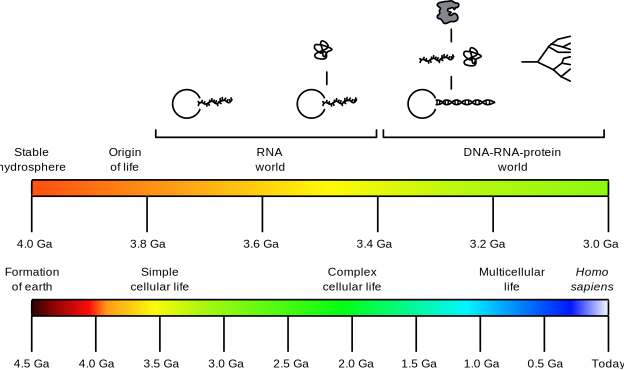
\includegraphics[width=.8\linewidth]{fig/rnaworld} % TODO: change image
	\caption{
		\textbf{RNA world.} The postulated rise and fall of the RNA world during the evolution of life, from early self-replicating RNA to complex, RNA-controlled metabolism, to the invention of translation, followed by diversification of all modern branches of life. Image from Horning (2011)\cite{horning_rnaworld_2011}.
%		\fbox{\color{red} TODO: combine images, rewrite the description.}
	}
	\label{fig:rnaworld}
\end{figure}

\subsection{Central dogma}
The central dogma describes the general flow of genetic information in almost all existing living cells: DNA is decoded to RNA, which in turn encodes proteins\cite{strachan_humanmoleculargenetics_2011}. Main processes involved in the central dogma are \textbf{transcription}, \textbf{splicing}, and \textbf{translation} (Figure \ref{fig:centraldogma}). 

\begin{figure}[htb!]
	\centering
	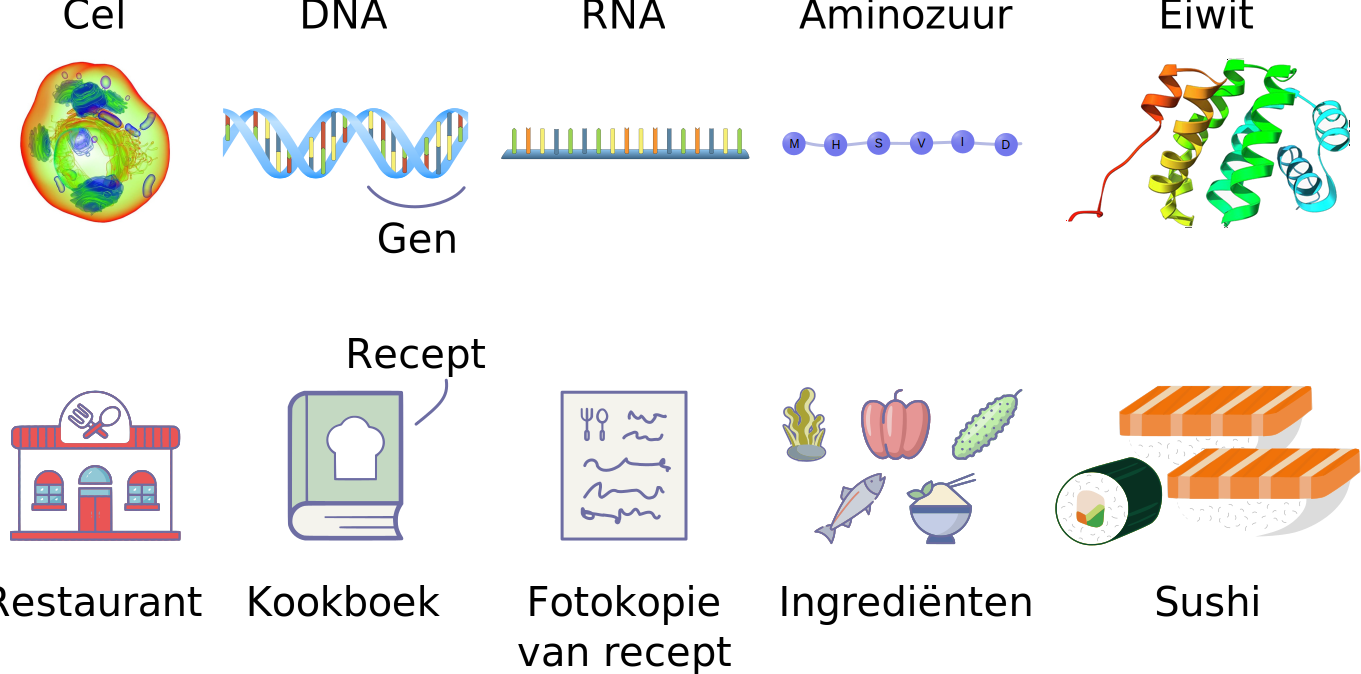
\includegraphics[width=.7\linewidth]{fig/central_dogma} % TODO: change image
	\caption{
		\textbf{Central Dogma.}
%		\fbox{\color{red} TODO: combine images, rewrite the description.}
	}
	\label{fig:centraldogma}
\end{figure}

During the process of \textbf{transcription} that takes place in the cell nucleus, a complementary RNA copy is transcribed from the template DNA. The initial RNA transcript is a precursor messenger RNA (pre-mRNA) that needs to undergo series of maturation steps to ultimately form the mature messenger RNA (mRNA). This maturation includes pre-mRNA \textbf{splicing} to remove non-protein coding intervening sequences (the introns) and to join the neighbouring protein-coding sequences (the exons). A single pre-mRNA can be alternatively spliced to generate multiple forms of mRNAs that will result in the production of multiple protein isoforms. This process of alternative splicing is essential to generate more than 100'000 different proteins starting from just 20'000 genes\cite{nilsen_expansioneukaryoticproteome_2010}.

The mature mRNA is then transported to the cytoplasm, where it engages with ribosomes to initiate \textbf{translation}. During this highly evolutionary conserved process, a chain of amino acids, known as the protein building blocks, is being synthesised. Each amino acid is specified by three nucleotides (a codon) in the mRNA, according to a nearly universal genetic code. After being released by the ribosomes, the translation product undergoes a variety of chemical modifications to form the final folded protein, the structure of which is determined by the sequence of different amino acids in the chain. In addition, polypeptides may be cleaved to yield more than one active polypeptide product. The structure of a protein determines its functionality, which includes catalysing biochemical reactions, providing structure, and transportation of molecules.


\subsection{Cell types}
Ever since Robert Hook first described the different structures of cells in 1665, biologists have been classifying cells by form and function.
The human body is said to contain more than 210 different cell types that are classified into four groups: epithelial, connective, muscle, and nervous. This however, is a major underestimation of the real number of cell types. Neurons, for instance, that are known to be extremely diverse, are estimated to reach numbers above 10,000 different types\cite{strachan_humanmoleculargenetics_2011}.

The concept of cell types eases reasoning and our understanding about many aspects of biology (e.g. the process of cell differentiation, cell-cell communication, cellular response to certain stimuli). Some cells are known to be highly specialised toward performing a particular function (e.g. memory B cells accelerate immune response by remembering previously encountered pathogens), or they can maintain a strong ability to differentiate into other cell types.

One common approach for understanding the functionality of a particular cell is to observe which molecules are present in the cell and to associate those set of molecules with functionality. Taking a snap shot of the protein or RNA transcript content in a particular cell, might already provide us with major insights into its functionality. However, in order to fulfil a particular task, the biochemical machinery of the cell gradually changes over time. Therefore it is highly informative to also consider the transition states between cell types and the dynamic processes involved therein.

\subsection{Cell dynamics and gene regulation}
Cells are dynamic entities that can gradually produce the molecules needed to acquire new functionality. The naturally occurring cell-to-cell variability happens at the level of gene expression. Gene expression itself can be controlled at different levels (Figure~\ref{fig:controlexpression}), one of which is gene regulation by transcription.

\begin{figure}[htb!]
	\centering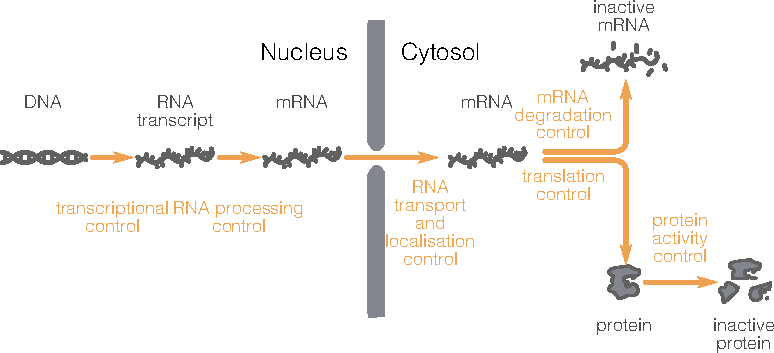
\includegraphics[width=.8\linewidth]{fig/control_gene_expression} % TODO: change image
	\caption{
		\textbf{Levels of controlling gene expression} can happen at the level of transcription, RNA processing (i.e. splicing), RNA transport and localization, mRNA translation, mRNA degradation and protein activity \cite{alberts_overviewgenecontrol_2002}.
	}
	\label{fig:controlexpression}
\end{figure}

According to the needs of a cell, different genes are being transcribed. Housekeeping genes are being expressed in essentially every cell, while other genes are cell type or tissue specific or may be expressed in response to developmental and environmental signals\cite{strachan_humanmoleculargenetics_2011}. 

Transcription factors (TFs) modulate the rate of gene transcription by binding and recruiting the transcriptional machinery to \emph{cis}-regulatory regions (enhancers, and silencers) that are typically located in the promotor region of target genes. These bindings may result in increased or decreased gene expression. 
There are several TF families of which members share structural characteristics (e.g. zinc finger, helix-loop-helix).

Many TFs are commonly present in virtually all cell types (e.g. NF-$\kappa$B), while others are specific for cells and developmental stages\cite{lambert_humantranscriptionfactors_2018}. Typically, the same TF can regulate the rate of transcription of many target genes in different cell types, indicating that these gene regulatory networks (GRNs) are dynamic. Moreover, the production of a specific molecule might require several gene regulatory cascades. Studying the active parts of a cell's GRN can thus reveal which dynamic processes are taking place within a cell.

% KDP: misschien interessant om over tumor heterogeniteit te spreken: waarvan we vroeger dachten dat homogene massa van cellen was, blijkt toch veel complexer te zijn --> nu mogelijk om met sc technieken te bestuderen?

\subsection{Profiling single cells}
Several technologies are now available to profile (i.e. observe) biomolecular components, allowing us to gain better understanding in the biological processes that take place within a cell. The single-cell "omics" technologies originated from the convergence of two different fields, \emph{"single-cell"} and \emph{"omics"}.

\subsubsection{Single-cell}
The earliest approach for measuring the abundance of a particular molecule in \emph{single cells} is the microscope.
Since its development by Coons et al. (1941), immunohistochemistry (IHC) has been instrumental in visualising proteins.\cite{coons_immunologicalpropertiesantibody_1941}. 
A cell can present a particular type of protein, also called an antigen, on its cell surface. In many multicellular organisms, antigens can stimulate the immune system to produce antibodies. IHC realises the visualisation of proteins by exploiting the principle of antibodies binding to specific antigens.

IHC (and many other biotechnologies) visualises antigen-antibody reactions by attaching particular molecules to the antibody, such as an enzyme that catalyses a colour-producing reaction, or a fluorescent chemical compound that can re-emit light upon excitation. The use of several colours (wavelengths) allows measuring expression levels of different antibodies simultaneously. Characterising cells in a semi-quantifiable way is labour intensive, however; since it involves acquiring an image of many cells and drawing a contour around each cell (called cell segmentation).
Modern implementations of IHC improve the throughput drastically by using robots and computer software to provide semi-automated image acquisition and cell segmentation\cite{theodosiou_automatedanalysisfish_2007}.

Flow cytometry\cite{fulwyler_electronicseparationbiological_1965} circumvents imaging and segmentation issues by measuring fluorescently labelled proteins as cells pass through a fluidic system.
Since cells need to be suspended in a buffer, flow cytometry is particularly useful for analysing non-adherent cells such as the many different immune cells in blood. However, many protocols already exist to extract viable single cells from tissues and tumours\cite{leelatian_preparingviablesingle_2017}.
Conventional flow cytometry devices enable to measure protein expression levels of millions of cells using up to eight different antibody fluorochromes simultaneously, while state-of-the-art instrumentation allows detection of up to 27 biomarkers simultaneously\cite{cossarizza_guidelinesuseflow_2017}.

Besides IHC and flow cytometry, many new technologies have been developed which allow quantifying expression levels of molecules in single cells (e.g. mass cytometry, single-cell quantitative polymerase chain reaction, fluorescence \emph{in situ} hybridization). All of these single-cell (non-omics) technologies are limited by the number of different molecules they measure, however. Selecting molecules of interest prior to analysis, makes the experiment biased towards the preconceptions of the experimenter.

\subsubsection{Omics}
On the other side of the spectrum are the so-called "omics" technologies. "Omics"\footnote{The etymology of "omics" is quite interesting\cite{yadav_wholenesssuffixomics_2007}.} is a collective term for profiling all molecules of a particular type in a high-throughput manner.
There are at least ten types of "omics". In this work, we mostly consider genomics, transcriptomics, proteomics, and regulomics. Genomics studies the complete DNA sequence of an organism's genome, while transcriptomics and proteomics study the RNA transcripts and proteins, respectively. Regulomics studies the regulatory molecules (e.g. genes, RNAs, proteins) which play a role in determining gene regulation.

Specific examples of omics technologies are whole genome sequencing to determine the DNA sequence of an organism, and RNA sequencing to profiles the sequence of RNA transcripts, both using next-generation sequencing technologies. A gene expression profile can be obtained by mapping the sequences of RNA transcripts to the genome.

Several high-throughput technologies have been developed to investigate proteomes in depth. The most commonly applied are mass spectrometry-based and gel-based techniques (e.g. differential in-gel electrophoresis).

% Je had proteomics technieken niet meer aangehaald. -> zie deze paperlink voor eventueel fig 1 of 2. Hoewel dit misschien niet je hoofdtopic is. https://academic.oup.com/chromsci/article/55/2/182/2333796

Typically for these methods, to capture enough material to generate a profile, numerous cells need to be pooled and lysed together, thereby granting the technology's name "bulk" omics.
Bulk omics is a major workhorse in molecular genetics and has applications in cancer research and in diagnostic screening of inheritable disorders.

Increasing evidence shows that cells are biomoleculary heterogeneous, even in very similar cell types\cite{hwang_singlecellrnasequencing_2018} (Figure~\ref{fig:bulk_vs_sc}A). Since a bulk profile is a population average (or rather, a summation), important cell-to-cell variability is not discernible (Figure~\ref{fig:bulk_vs_sc}B). 

\begin{figure}[htb!]
	\centering
	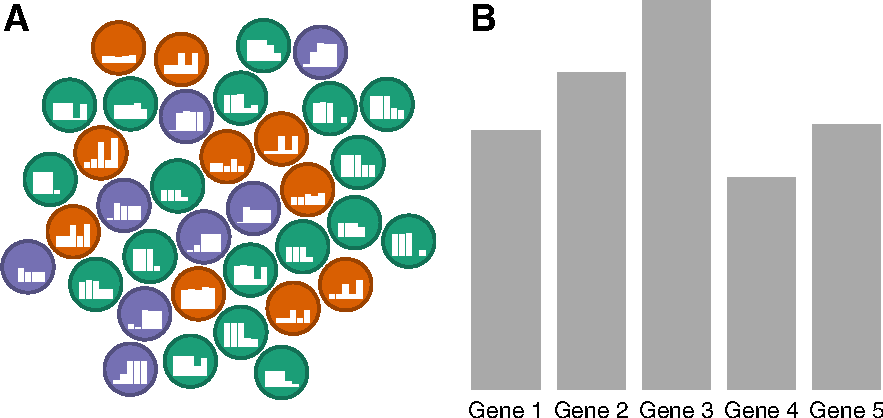
\includegraphics[width=\LARgefigure]{fig/bulk_vs_sc} 
	\caption{
		\textbf{The 'masking' effect of bulk omics.} 
		\textbf{A:} Cells from several subpopulations are incorrectly assumed to be homogeneous and are profiled with a single bulk omics experiment.
		\textbf{B:} The signals from the different subpopulations are masked. The resulting profile is dissimilar from the majority of cells it is supposed to represent.
	}
	\label{fig:bulk_vs_sc}
\end{figure}

\subsubsection{Single-cell omics}
Comparing single-cell technologies with omics technologies shows that they have both clear advantages but also significant drawbacks (Figure \ref{fig:profiling_convergence}A). Single-cell biology allows profiling thousands or even millions of cells, but only for a select number of genes. On the other hand, omics biology provides a broader view -- since genes do not need to be selected beforehand -- but is a profile of ensemble of cells and thus masks important cellular heterogeneity.

Advances in microvolume sequencing allowed profiling the transcriptome at single-cell resolution, thereby bringing single-cell biology and omics together to create single-cell omics. During the decade that followed, the number of single-cell omics technologies has sky-rocketed, allowing to profile >100'000 cells\cite{svensson_exponentialscalingsinglecell_2018} and measuring other levels of information (e.g. protein abundance and spatial location) \cite{moudgil_multimodalscrnaseq_2019}.

\begin{figure}[htb!]
	\centering
	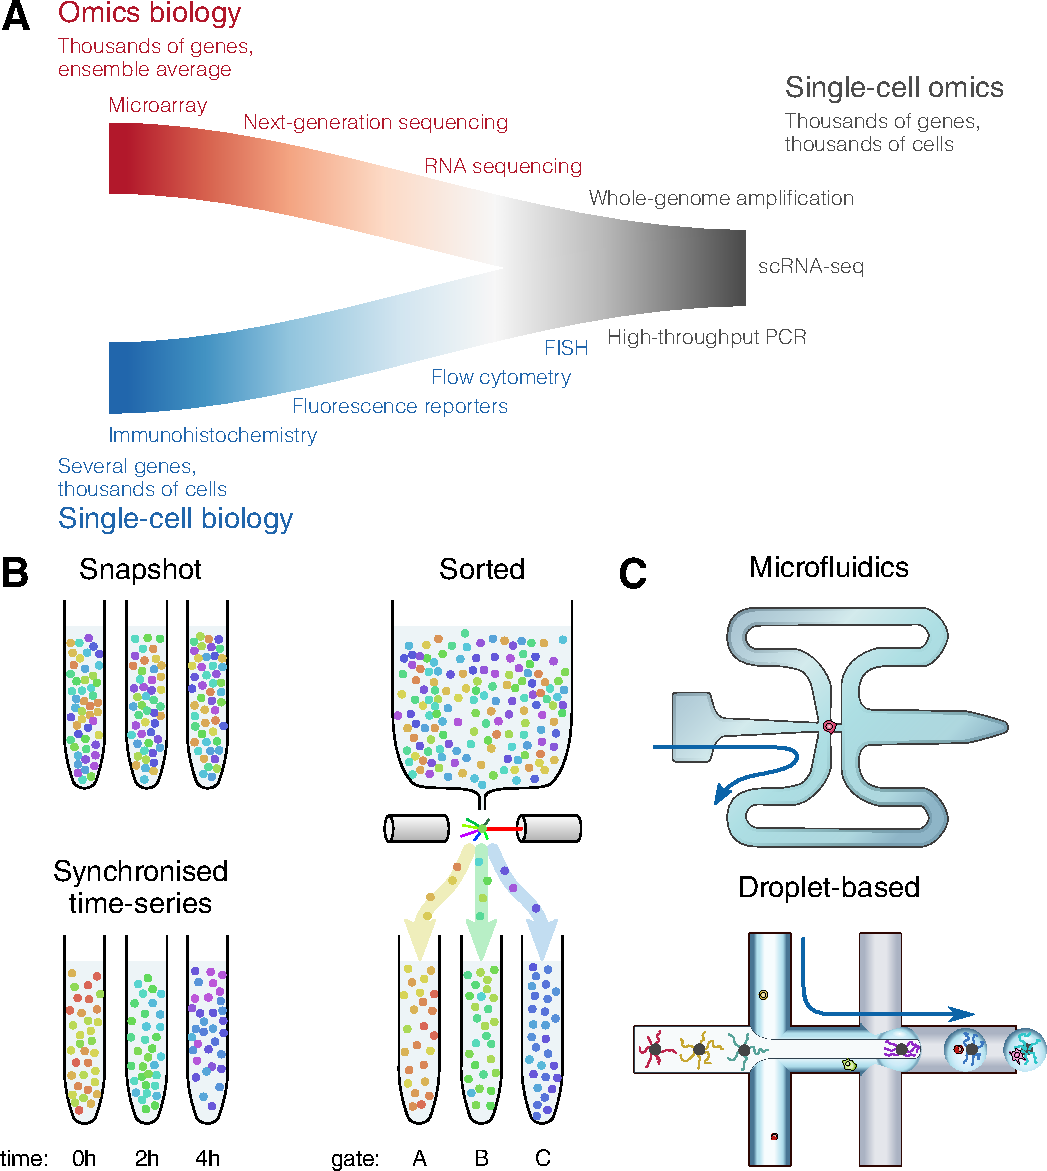
\includegraphics[width=.7\linewidth]{fig/scomics_2.pdf} 
	\caption{
		\textbf{A:} Convergence of single-cell and omics biology.
		\textbf{B:} Different approaches for sampling cells with decreasing levels of cellular heterogeneity within the different sub-populations: snapshot, time-series, sorted.
		\textbf{C:} Two common single-cell RNA sequencing technologies. Microfluidics systems let cells travel through nanometer scale tubing, capturing individual cells at intersections. Droplet-based systems encapsulate individual cells in droplets.
	}
	\label{fig:profiling_convergence}
\end{figure}

% could be expanded with information on how to isolate single cells and how to profile them
% see https://www.nature.com/articles/s12276-018-0071-8
% seems interesting as well: 10.1146/annurev-biodatasci-080917-013452

In this work, unless noted otherwise, we will be working with transcriptomics data resulting from a single-cell RNA-sequencing experiment (scRNA-seq). The workflow of generating scRNA-seq profiles is as follows. Same as other single-cell (non-omics) profiling methods, cells first need to be isolated (Figure~\ref{fig:profiling_convergence}B). Different sampling techniques yield different levels of information about cellular state. By now, many protocols for extracting and tagging RNA from single cells have been developed\cite{svensson_exponentialscalingsinglecell_2018}, the most popular of which are based on microfluidics or droplets (Figure~\ref{fig:profiling_convergence}C). By sequencing the trancripts and the attached unique cell identifier tags, each read can be mapped and tallied up. scRNA-seq data can thus be summarised in a matrix, where each column represent a single cell, each row a gene, and each value represents the number of transcripts that were sequenced for that gene and cell.

The rapidly advancing field of single-cell omics harbours exceptional opportunities to discover new aspects of biology and redefine existing knowledge. Some of these opportunities lie in efforts like the HCA consortium\cite{regev_humancellatlas_2018}. They have set out to redefine all human cell types in both terms of their gene expression and location, and as well as the developmental trajectories connecting the different cell types. As part of this endeavour, the consortium will likely profile the whole transcriptomes of tens or even hundreds of millions of cells\cite{humancellatlasconsortium_humancellatlas_2018}. 

\section{Computational tools}
Whole-genome profiling at single-cell level allows new types of analyses with which to study cellular heterogeneity at a hitherto unseen throughput. 
The new types of analyses permitted by single-cell omics present several computational challenges\cite{stegle_computationalanalyticalchallenges_2015, yuan_challengesemergingdirections_2017, chen_singlecellrnaseqtechnologies_2019}. This necessitates the development of novel computational tools, either because the problem statement of the performed analysis is completely novel, or to adapt existing methodology to new data characteristics -- dimensionality and noise. 

scRNA-seq data is typically very sparse -- while the human genome has more than 20'000 genes, they only contain non-zero values of a few thousand genes (typically <4'000). This is partially due to cells being specialised in particular functions and thus they do not need proteins of every time, but also due to RNA transcription occurring in bursts rather than continuously\cite{nicolas_whatshapeseukaryotic_2017}. This contributes to the high levels of noise seen in scRNA-seq data: no two cells have the same set of non-zero genes. 

Over the past five years, already 450 new tools have been developed to perform various analyses of single-cell omics data\cite{zappia_exploringsinglecellrnaseq_2018}, taking into account the specific noise characteristics. The most frequent types of analyses are detailed in the following subsections.

\subsection{Dimensionality reduction}
Single-cell omics datasets are usually one or more high-dimensional matrices, containing between M = $10^3$ to $10^5$ cells and typically about N = $10^3$ to $10^4$ genes (Figure~\ref{fig:comp_tools_dimred}A). The dimensionality of such datasets is typically too high for humans to interpret manually and for most modelling algorithms to tackle directly. 
Moreover, in reality, the intrinsic dimensionality of biological systems is probably much lower. For example, a differentiating hematopoietic cell could be described by just three dimensions: the first two dimensions lays out the hematopoietic lineage tree, and a third dimension allows for reprogramming between branches to occur.

Dimensionality reduction (DR) methods transform high-dimensional data into a meaningful low-dimensional representation. DR methods have two main target audiences; computers -- to construct a K-dimensional (with K $\ll$ M) representation of the data such that pairwise distances between different samples are retained as well as possible (Figure~\ref{fig:comp_tools_dimred}B); and humans -- to obtain a visual overview of the data (Figure~\ref{fig:comp_tools_dimred}C).

Each dimension frequently corresponds to one or more modules of co-expressed genes.  The reduced space can be interpreted in way analogous to Waddington’s epigenetic landscapes\cite{waddington_strategygenesdiscussion_1957,ferrell_bistabilitybifurcationswaddington_2012,rebhahn_animatedlandscaperepresentation_2014}, where the landscape dictates the possible states a cell can reside in, and transitions between states correspond to dynamic cellular processes, such as cell differentiation. 

\begin{figure}[htb!]
	\centering
	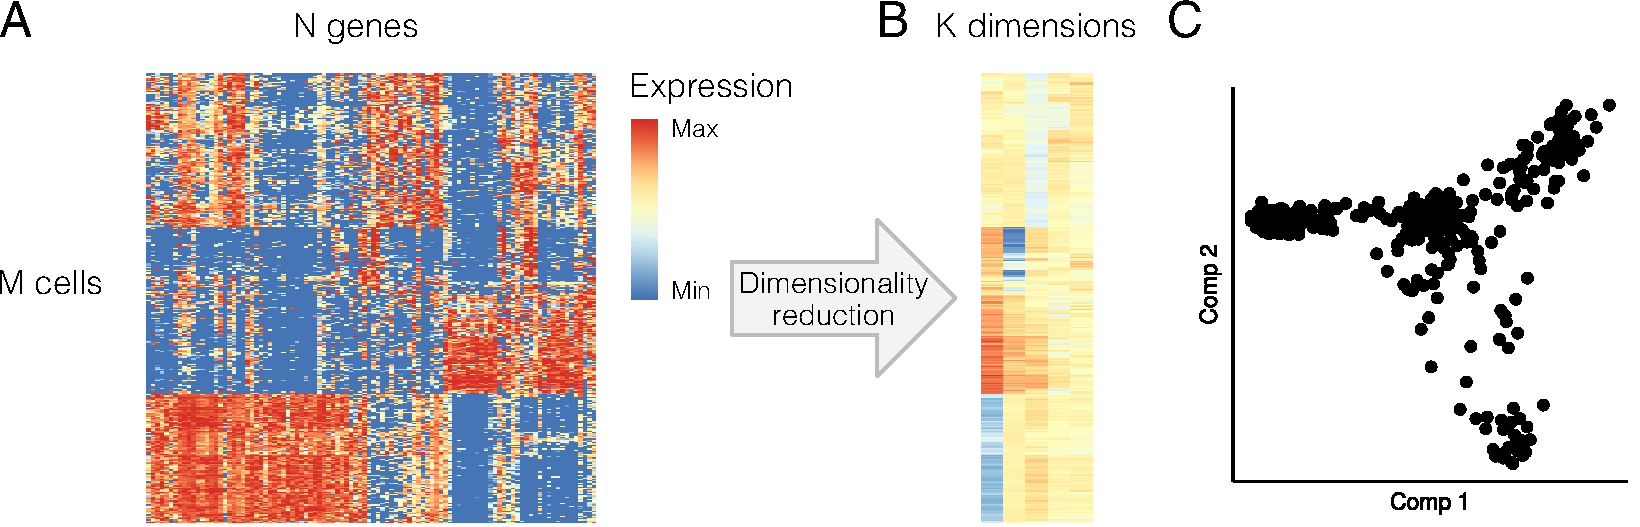
\includegraphics[width=\linewidth]{fig/comptools2/comptool_1_dimred.pdf} 
	\caption{
		\textbf{Dimensionality reduction for single-cell omics data.}
		\textbf{A:} A heatmap visualisation of an scRNA-seq expression dataset of fibroblasts being reprogrammed to neuron cells\cite{treutlein_dissectingdirectreprogramming_2016}. Only the most variable 
		\textbf{B:} The reduced space is a M$\times$K-dimensional matrix which attempts to conserve the cellular heterogeneity of the original space as well as possible.
		\textbf{C:} A dot plot of the first two components of the reduced space provides a global overview of the cells in the dataset. Colouring the dots according to prior information (e.g. cell type) or gene expression provides insight into the cellular heterogeneity within the dataset.
	}
	\label{fig:comp_tools_dimred}
\end{figure}

DR methods can be classified into two main categories, feature projection-based and manifold learning\cite{engel_surveydimensionreduction_2012}. 

Projection-based DR methods aim to perform a transformation of the data while preserving the pairwise distances between samples as much as possible. Examples of commonly used projection-based DR methods in single-cell omics are Principal Component Analysis\cite{pearson_liiilinesplanes_1901} (PCA) and Multi-Dimensional Scaling\cite{kruskal_multidimensionalscalingoptimizing_1964} (MDS). 

Manifold learning DR methods reconstruct a higher-order structure in the original space (e.g. a graph or a grid), visualising the structure in a lower-dimensional space, and mapping the original samples to the lower-dimensional space. Manifold learning can be an iterative optimisation process using a predefined criterion. Examples of manifold learning techniques are t-distributed Stochastic Neighbor Embedding\cite{vandermaaten_visualizingdatausing_2008} (t-SNE), Diffusion Maps\cite{nadler_diffusion_2005,coifman_diffusionmaps_2006} and Uniform Manifold Approximation and Projection\cite{mcinnes_umapuniformmanifold_2018} (UMAP). 

For scalability reasons, this work mostly makes use of Landmark MDS\cite{silva_globallocalmethods_2002,lee_landmarkmdsensemble_2009} (LMDS) with a Spearman rank correlation distance metric. LMDS is an extension of classical MDS, but rather than calculating a complete distance matrix between all pairs of cells, a set of landmark cells is sampled, only the distances between a set of landmarks and the samples are calculated. 

\subsection{Clustering}
To learn about the different cellular states within a population of cells, clustering methods divide up the cells into separate groups of highly similar cells (Figure~\ref{fig:comp_tools_cluster}A). 
By visualising gene expression of known genes involved in the cell types of interest, the clusters can be annotated (Figure~\ref{fig:comp_tools_cluster}B). 

\begin{figure}[htb!]
	\centering
	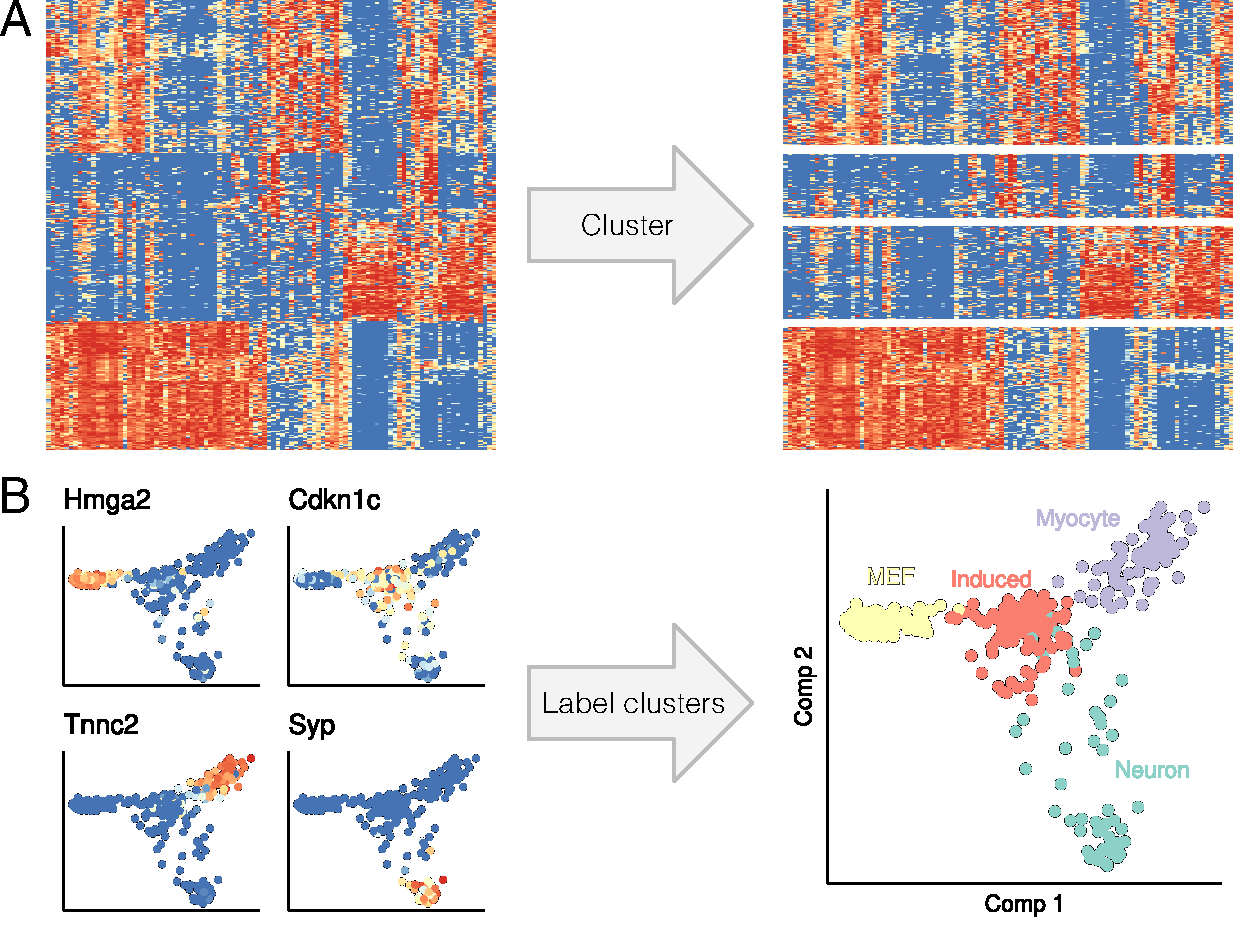
\includegraphics[width=.6\linewidth]{fig/comptools2/comptool_2_clustering.pdf} 
	\caption{
		\textbf{Clustering for single-cell omics data.}
		\textbf{A:} Clustering methods group cells with similar omics profiles together. 
		\textbf{B:} By overlaying gene expression levels on a dimensionality reduction, the clusters can be annotated to allow better interpretation of the cellular heterogeneity.
	}
	\label{fig:comp_tools_cluster}
\end{figure}


Usually, the number of clusters is determined by the user, either as a direct parameter (e.g. $k$-means\cite{lloyd_leastsquaresquantization_1982}) or an indirect parameter (e.g. a height cutoff in hierarchical clustering). In some exceptional cases, the number of clusters is strictly determined by the data itself and cannot be altered with a parameter (e.g. Louvain clustering\cite{blondel_fastunfoldingcommunities_2008}).

Clustering methods used in this work are mostly restricted to $k$-Means for clustering low-dimensional spaces and Louvain for clustering networks, since both are highly scalable with respect to the number of cells.

\subsection{Trajectory inference}
While clustering methods divide cells into distinct groups, trajectory inference (TI) methods acknowledge that cells are dynamic entities which transition from once cellular state to another via various dynamic processes. Rather than making distinct groups, TI methods allow studying dynamic processes by reconstructing the topology of a dynamic process as a trajectory, and map the cells onto that trajectory. A trajectory is a graph where the nodes represent noteworthy cellular states, and each cell is predicted to be progressing along transitions between the different states (Figure~\ref{fig:comp_tools_ti}A).

A trajectory can be visualised as a graph to better highlight the topology of the trajectory(Figure~\ref{fig:comp_tools_ti}A middle), as a heatmap to better depict the changes in gene expression along the different transitions (Figure~\ref{fig:comp_tools_ti}A right), or may be embedded in a dimensionality reduction of the cells to better demonstrate cellular heterogeneity along the trajectory (Figure~\ref{fig:comp_tools_ti}B right). Similar to clustering, by colouring the cells according to the expression of genes known to be involved in the dynamic process of interest, the milestones in the trajectory can be annotated (Figure~\ref{fig:comp_tools_cluster}B). 

\begin{figure}[htb!]
	\centering
	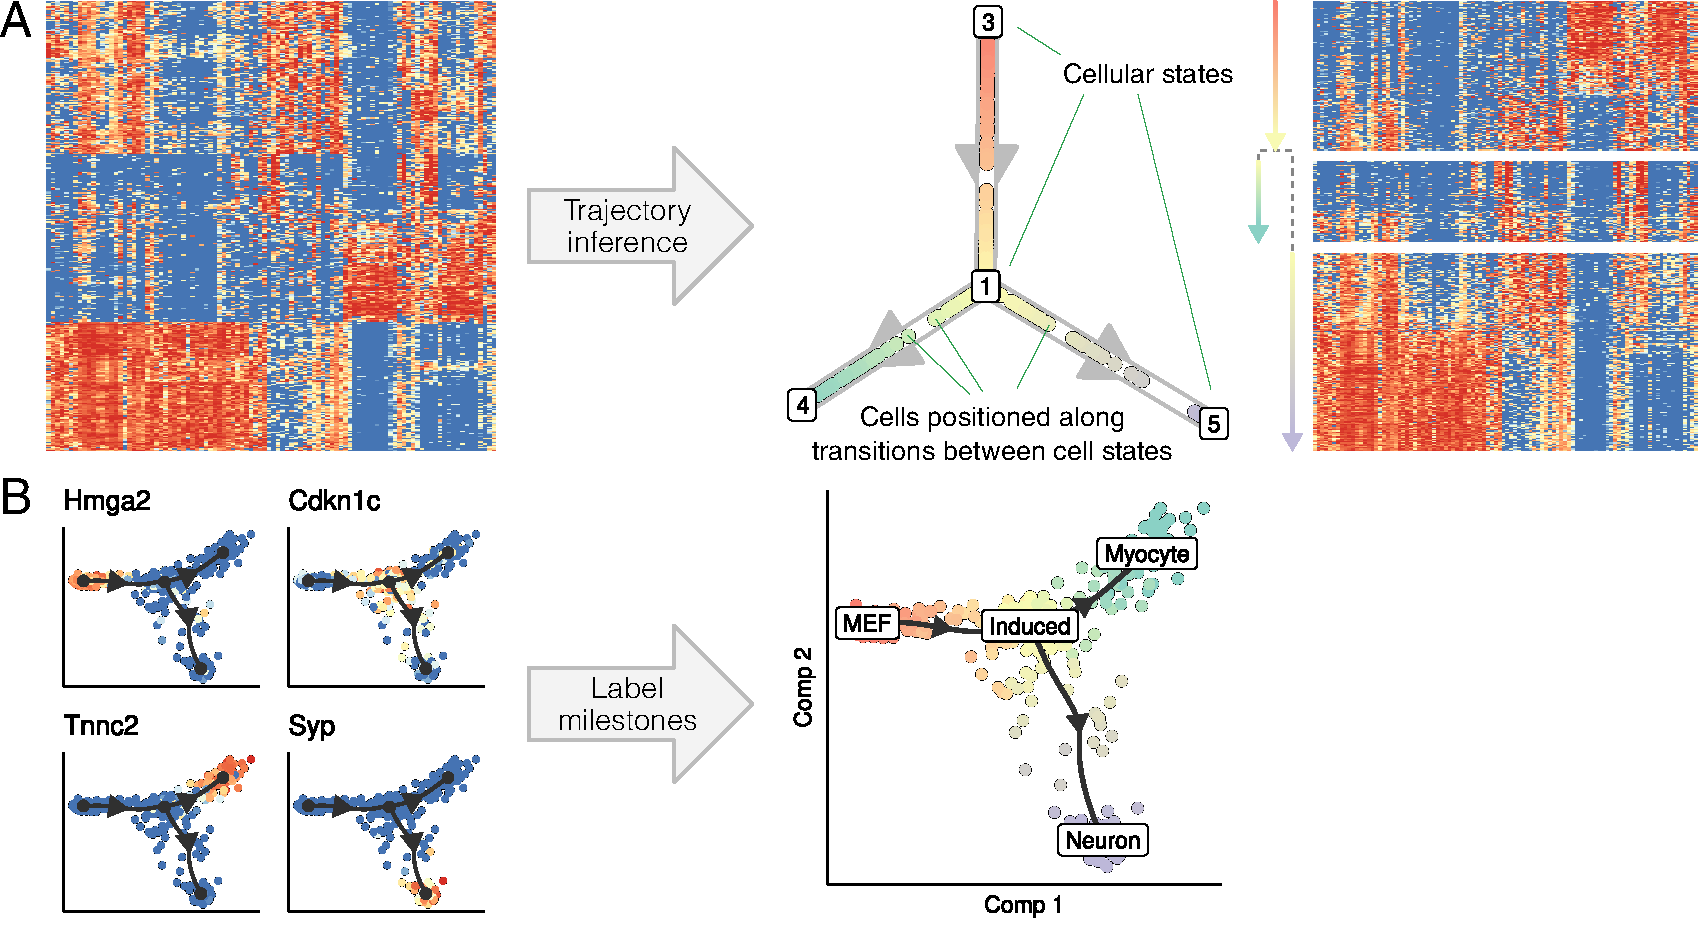
\includegraphics[width=.9\linewidth]{fig/comptools2/comptool_3_trajectoryinference.pdf} 
	\caption{
		\textbf{Trajectory inference for single-cell omics data.}
		\textbf{A:} During a dynamic process cells pass through several transitional states, characterized by different waves of transcriptional, morphological, epigenomic and/or surface marker changes\cite{enver_stemcellstates_2009}. TI methods provide an unbiased approach to identifying and correctly ordering different transitional stages. 
		\textbf{B:} By overlaying gene expression levels on a dimensionality reduction, the milestones can be annotated to allow better interpretation of the cellular heterogeneity.
	}
	\label{fig:comp_tools_ti}
\end{figure}

A lot of TI methods use similar algorithms to be able to infer a trajectory. By breaking down each method into its set of core algorithms, we can create a map of TI methodology\cite{cannoodt_computationalmethodstrajectory_2016} (Figure~\ref{fig:ti_metro}A), which is divided into two major classes.
In the first step, dimensionality reduction techniques such as manifold learning, clustering, or graph-based methods are used to convert the dataset to a more simplified representation. This representation of the data then allows the trajectory itself to be more easily modelled in a second step. In this second step, the trajectory is modelled within the data using graph-based or curve-based approaches, after which the cells themselves can be ordered using a variety of methods.

A common way to classify TI methods is by the types of trajectories they can infer\cite{saelens_comparisonsinglecelltrajectory_2019} (Figure~\ref{fig:ti_metro}B). About half of TI methods specialise in inferring linear or cyclic trajectories (i.e. they order the cells). Others model the trajectory as a rooted tree, allowing for one or more bifurcations to occur. Only a few methods are able to infer more generalised trajectories containing disconnected subgraphs or cycles.

\begin{figure}[htb!]
	\centering
	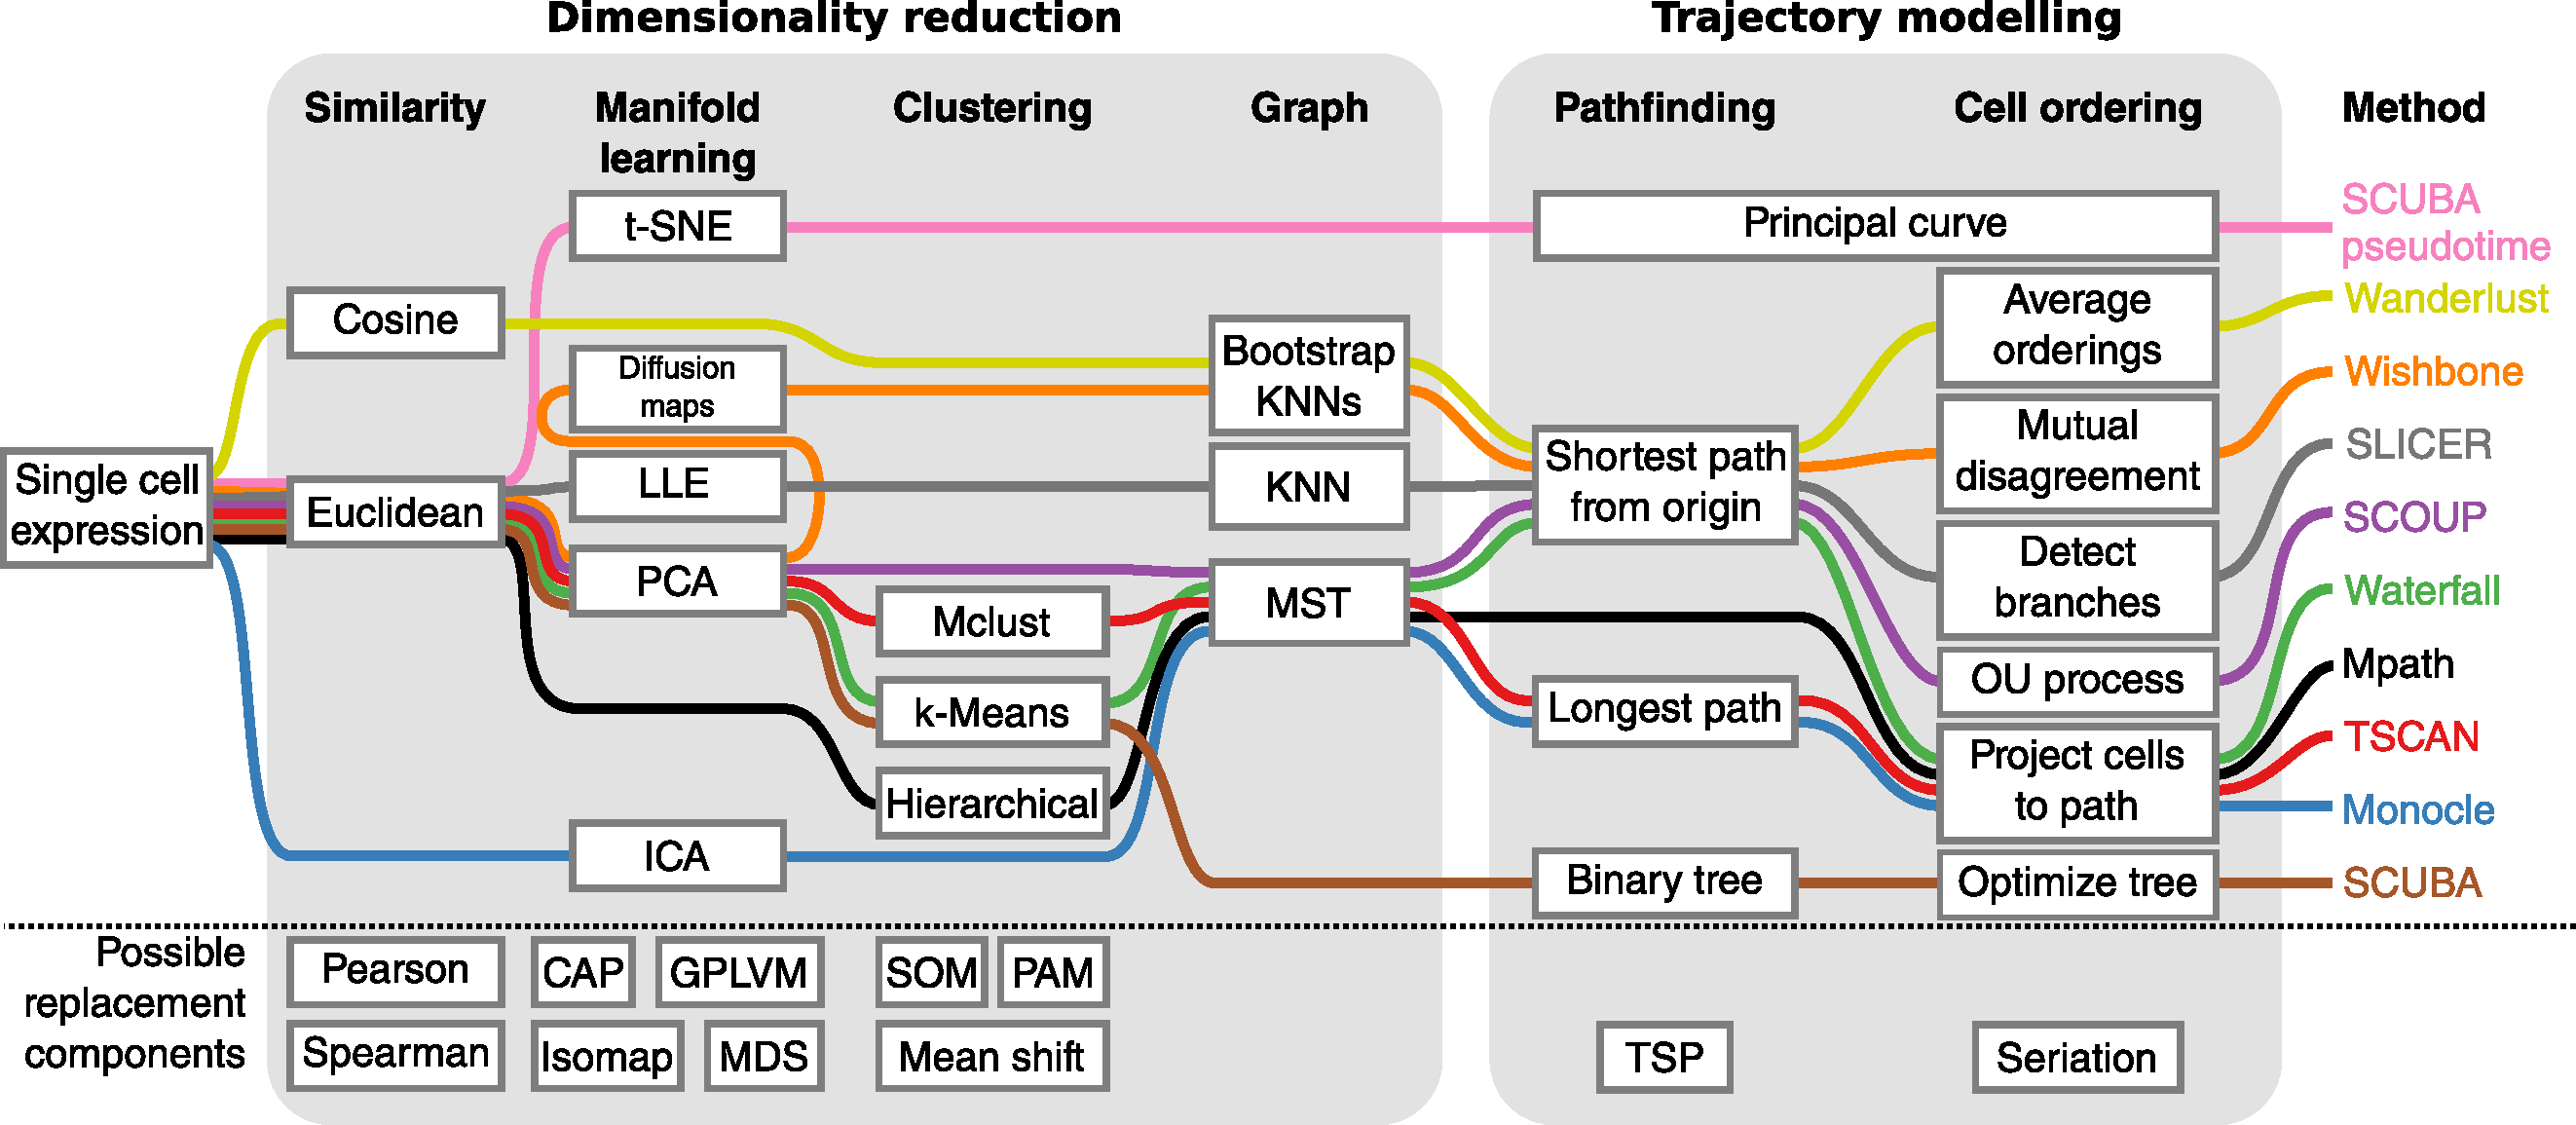
\includegraphics[width=.9\linewidth]{fig/ti_metro} 
	\caption{
		\textbf{TI methods use several common building blocks and can be organized in a unifying modular framework.} 
		\textbf{A:} Most TI methods consist of two major steps, dimensionality reduction and trajectory modelling. TI methods   require some form of dimensionality reduction in order to summarise cell heterogeneity in a lower dimensional space. Subsequently, a trajectory modelling step then operates in this reduced space, aiming to identify cell states, constructing a trajectory through the different states, and projecting the cells back on to the trajectory. 
		\textbf{B:} TI methods can be classified according to the trajectory topologies they can infer.
	}
	\label{fig:ti_metro}
\end{figure}


\subsection{Differential expression}
Given that cells are split up into groups differential expression (DE) methods ranks genes based on whether their expression is significantly higher or lower in one group in comparison to the others. This grouping can be based on prior information or an upstream clustering method. DE methods are useful for summarising the main differences between different groups of cells more compactly (Figure~\ref{fig:comp_tools_de}A) in comparison to when groups are compared without gene prioritisation (Figure~\ref{fig:comp_tools_cluster}A). 

Trajectory differential expression (TDE) is an extension of DE where instead genes are prioritised according to whether their gene expression changes smoothly but significantly along a parts of a trajectory (Figure~\ref{fig:comp_tools_de}). 

\begin{figure}[htb!]
	\centering
	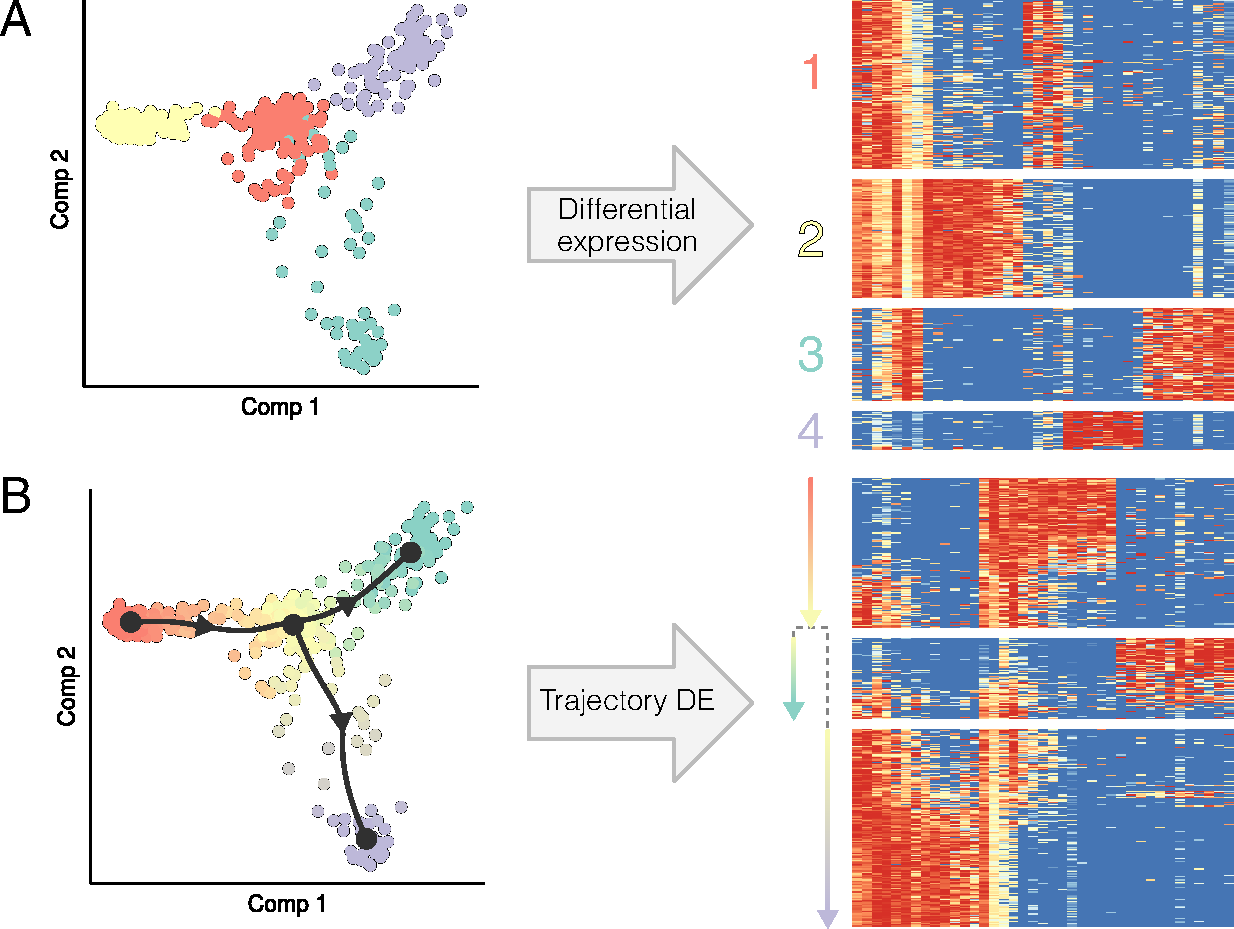
\includegraphics[width=.6\linewidth]{fig/comptools2/comptool_4_differentialexpression.pdf} 
	\caption{
		\textbf{Differential expression for single-cell omics data.}
		\textbf{A:} Differential expression methods prioritises genes that are expressed significantly higher or lower in particular given groups.
		\textbf{B:} Trajectory differential expression prioritises genes that change smoothly but significantly along particular transitions in a trajectory.
	}
	\label{fig:comp_tools_de}
\end{figure}

\subsection{Network inference}
One of the central cellular processes underlying development is transcriptional regulation. 	
Modeling the dynamics of gene regulation is therefore essential to better understand why a cellular dynamic processes progresses through several steps, and what goes wrong in the case of disease.

Network inference (NI) methods predict which genes are regulated by which transcription factors (Figure~\ref{fig:comp_tools_ni}). The output of a network inference is thus a graph, where nodes represent genes and edges denote a regulatory interaction between a regulator and a target gene. Interactions typically have two properties: its regulatory strength (a positive real value) and its effect (promoting or repressing).

Before single-cell omics, these methods rely on multiple experiments, amongst which perturbation and time-series experiments, to predict the effect each transcription factor has on the up- or downregulation of a gene. One of the main advantages of single-cell omics is the heterogeneity between cells caused by naturally occurring biological randomness\cite{padovan-merhar_usingvariabilitygene_2013} can be exploited to infer regulatory interactions between TFs and their target genes at much lower costs. 

\begin{figure}[htb!]
	\centering
	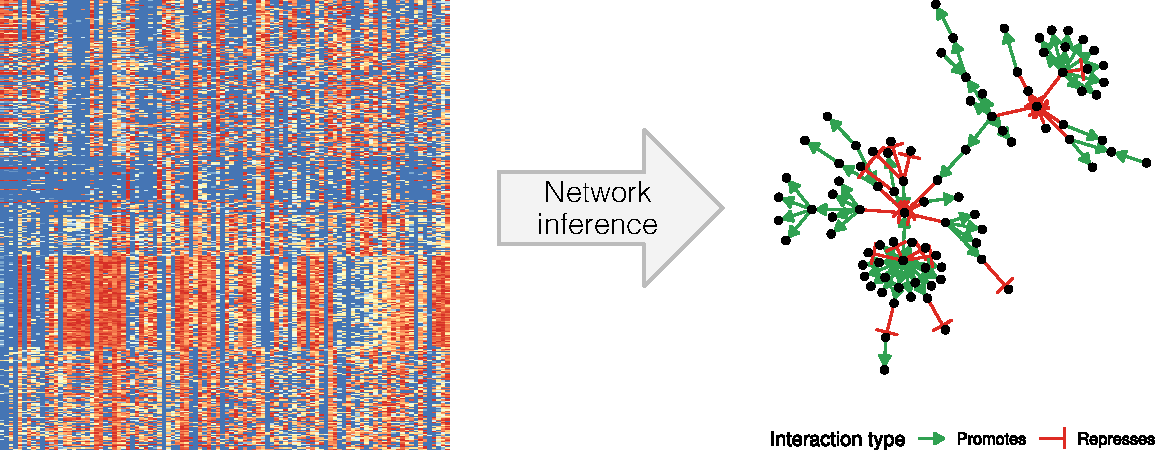
\includegraphics[width=.6\linewidth]{fig/comptools2/comptool_5_networkinference.pdf}
	\caption{
		\textbf{Network inference for single-cell omics data.}
	}
	\label{fig:comp_tools_ni}
\end{figure}



\section{Research context and objectives} \label{sec:research_objectives}
Recent technological advancements in profiling single cells are having significant repercussions in many fields of biology. Profiling thousands of individual cells in a genome-wide manner provides opportunities to study cell heterogeneity and dynamics, for example inferring mechanisms for cellular development or intercellular communication. 
Hundreds of new software tools were developed\cite{zappia_exploringsinglecellrnaseq_2018} to perform these new types of analyses, or to fit existing analytical tools to deal with new data characteristics (e.g. differential expression, dimensionality reduction, normalisation). 

One major shortcoming during the advent of single-cell omics was that the majority of newly developed computational tools were not quantitatively and comparatively evaluated. Rather, they relied on anecdotal evidence to demonstrate its usefulness. This issue is not the result of the tool developer's malevolence, but instead of the lack of data required to perform such comprehensive benchmarks.
%TODO: also mention guidelines for users.

Uncontrolled development of software tools without comprehensive benchmarking poses serious problems. 
For one, it slows down scientific progress. Every end-user needs to make a large commitment researching the domain in order to make an informed decision of which tool to use, or risk a higher incidence of false positive discoveries (either way, valuable resources are being wasted). In addition, it also negatively impacts the credibility of the field, thus discouraging potential users or researchers from entering.

In this work, we aim to speed up scientific progress in single-cell omics by providing tools both for end-users and developers alike. For developers of computational approaches, we provide tools and guidelines for benchmarking their method on real and synthetic data. For end-users we develop new tools and guidelines for analysing dynamic processes by inferring trajectories and gene regulatory networks. Our specific scientific objectives are discussed in the following chapters.

\begin{itemize}
	\item We \textbf{develop benchmarking strategies} for assessing the performance of computational tools constrained by low availability of novel types of real single-cell data (Chapter~\ref{chap:dyngen}). \textit{In silico} simulations of individual cells are used to help kick-start emerging domains much more safely and allow anticipation of future technological developments by already developing computational tools.
	\item We apply this strategy to \textbf{perform a comparison of TI methods} (Chapter~\ref{chap:dynbenchmark}). Trajectory inference is one of the largest categories of all the novel single-cell omics tools, yet a comprehensive and quantitative study of the advantages and disadvantages of the numerous tools was hitherto lacking. We provide a set of guidelines for end-users wishing to infer trajectories. Our pipeline, datasets, metrics, and containerised wrappers of TI methods are made publicly available for developers to use.
	\item We develop \textbf{a toolkit to infer, visualise and interpret single-cell trajectories} using more than 50 different TI methods (Chapter~\ref{chap:dyno}). dyno provides downstream analysis such as: visualising a trajectory in a low-dimensional space or a heatmap, detecting genes differentially expressed at different stages of the tragectory, comparing multiple trajectories in a common dimensionality reduction, and manipulating the trajectory (e.g. adding directionality or adding annotation).
	\item We introduce a TI method specialised in \textbf{inferring linear trajectories} (Chapter~\ref{chap:scorpius}). Despite linear TI being the most simple but commonly used form of trajectory inference, the benchmark demonstrated that most TI methods are not capable of producing accurate models of linear datasets.
	\item We develop an algorithm for  \textbf{inferring gene regulatory interactions at a single-cell level} (Chapter~\ref{chap:bred}). We demonstrate our NI methodology by inferring regulatory interactions for 22'122 hematopoietic cells, as well as for 14'963 bulk profiles of cancer tumours.
	\item We provide a tool for  \textbf{analysing the topological properties of large, evolving networks} and use this to iteratively optimise GRN predictions (Chapter~\ref{chap:incgraph}).
	\item We reflect on \textbf{challenges in performing self-assessments of TI methods} (Chapter~\ref{chap:selfassessment}).
	Reproducability problems of TI methods are partially due to low rates of quantitative self-assessment. We look at 75 manuscripts of TI methods and identify key challenges the authors had in benchmarking their tool. For each of these challenges, we provide a summary of how we and others have successfully tackled these challenges, in order to spur developers to perform more self-assessments.
	\item Finally, we \textbf{summarise our experience in benchmarking computational methods} by providing a list of essential guidelines in benchmarking computational tools (Chapter~\ref{chap:guidelines}).
\end{itemize}



%%%%%%%%%%%%%%%%%%%%%%%%%%%%%%%%%
%%%        CH2: DYNGEN        %%%
%%%%%%%%%%%%%%%%%%%%%%%%%%%%%%%%%
\newpage{\thispagestyle{empty}\cleardoublepage}
\chapter{dyngen: simulating single cells} 
\chaptermark{dyngen: simulating single cells}
\label{chap:dyngen}
\graphicspath{{./ch2_dyngen/}}
% DYNGEN CONTENT

%\begin{quote}
%	\textbf{Abstract:} 
%\end{quote}

\section{Introduction}
Continuous technological advancements to single-cells omics are having profound 
effects on how researchers can validate biological hypotheses. 
Early experimental technologies typically only allowed profiling a single modality (e.g. DNA sequence, 
RNA or protein expression). However, recent developments permit profiling multiple modalities simultaneously,
and every modality added allows for new types of analyses that can be performed.

This presents method developers with a problem. The majority of the 250+ peer-reviewed computational tools for analysing single cell omics data were published without a quantitative assessment of the accuracy of the tool. This is partially due to low availability of suitable benchmarking datasets; even if there are sufficient suitable input datasets available, these are often not accompanied by the necessary metadata to serve as ground-truth for a benchmark.

Here, synthetic data plays a crucial role in asserting minimum performance requirements for novel tools in anticipation of adequate real data. Generators of scRNA-seq data (e.g. splatter \cite{zappia_splattersimulationsinglecell_2017}, powsimR \cite{vieth_powsimrpoweranalysis_2017}, PROSSTT \cite{papadopoulos_prossttprobabilisticsimulation_2018} and SymSim \cite{zhang_simulatingmultiplefaceted_2019}) have already been widely used to explore the strengths and weakness of computational tools, both by method developers \cite{street_slingshotcelllineage_2018,parra_reconstructingcomplexlineage_2018,lummertzdarocha_reconstructioncomplexsinglecell_2018,lin_scclassifyhierarchicalclassification_2019} and independent benchmarkers \cite{duo_systematicperformanceevaluation_2018,saelens_comparisonsinglecelltrajectory_2019,soneson_biasrobustnessscalability_2018}.
However, a limitation of scRNA-seq profiles generators is that they would require significant methodological alterations to add additional modalities.

An ideal experiment would be able to observe all aspects of a cell, including a full history of its 
molecular states, spatial positions and environmental interactions \cite{stuart_integrativesinglecellanalysis_2019}.
While this falls outside the reach of current experimental technologies, generating synthetic data in anticipation of new experimental technologies would allow already developing the next wave of computational tools.

We introduce \texttt{dyngen}, a multi-modality simulator of single cells and their dynamics (Figure \ref{fig:showcase}A). A cell is simulated using Gillespie's Stochastic Simulation Algorithm (SSA) \cite{gillespie_exactstochasticsimulation_1977} where a cell consists of a set of molecules. Throughout a simulation, reactions (e.g. transcription, splicing) modify the abundance of these molecules, and the likelihood of a reaction occurring is again dependent on molecule abundance.

By simulating a cell over time in terms of its molecular state and the reactions that are allowed to occur, the simulator is more extendible to new modalities or experimental procedures (Figure~\ref{fig:showcase}B). We demonstrate \texttt{dyngen}'s flexibility by simulating snapshot, time-series and pertubation experiments, allowing to benchmark a wide variety of computational tools such as trajectory alignment and differential network inference methods.

\begin{figure}[htb!]
	\centering
	\includegraphics[width=\linewidth]{fig/showcase_4} 
	\caption{
		\textbf{Showcase of \texttt{dyngen} functionality.} 
		\textbf{A:} 
		\textbf{B:} Evaluating different types of computational tools requires simulating different types of experiments and extracting different layers of information from the simulation.
	}
	\label{fig:showcase}
\end{figure}

\section{Results}

A cell consists of a set of molecules, the abundance of which are affected by a set of reactions: transcription, splicing, translation, and degradation (Figure \ref{fig:simplecyclic}A). 
A gene regulatory network (GRN) define the reactions that are allowed to occur (Figure \ref{fig:simplecyclic}B), and is constructed such that a cell will develop over time (Figure \ref{fig:simplecyclic}C--D).
The likelihood of a reaction occurring is a function of the abundance of key molecules involved in each reaction (Figure \ref{fig:simplecyclic}E).

\begin{figure}[htb!]
	\centering
	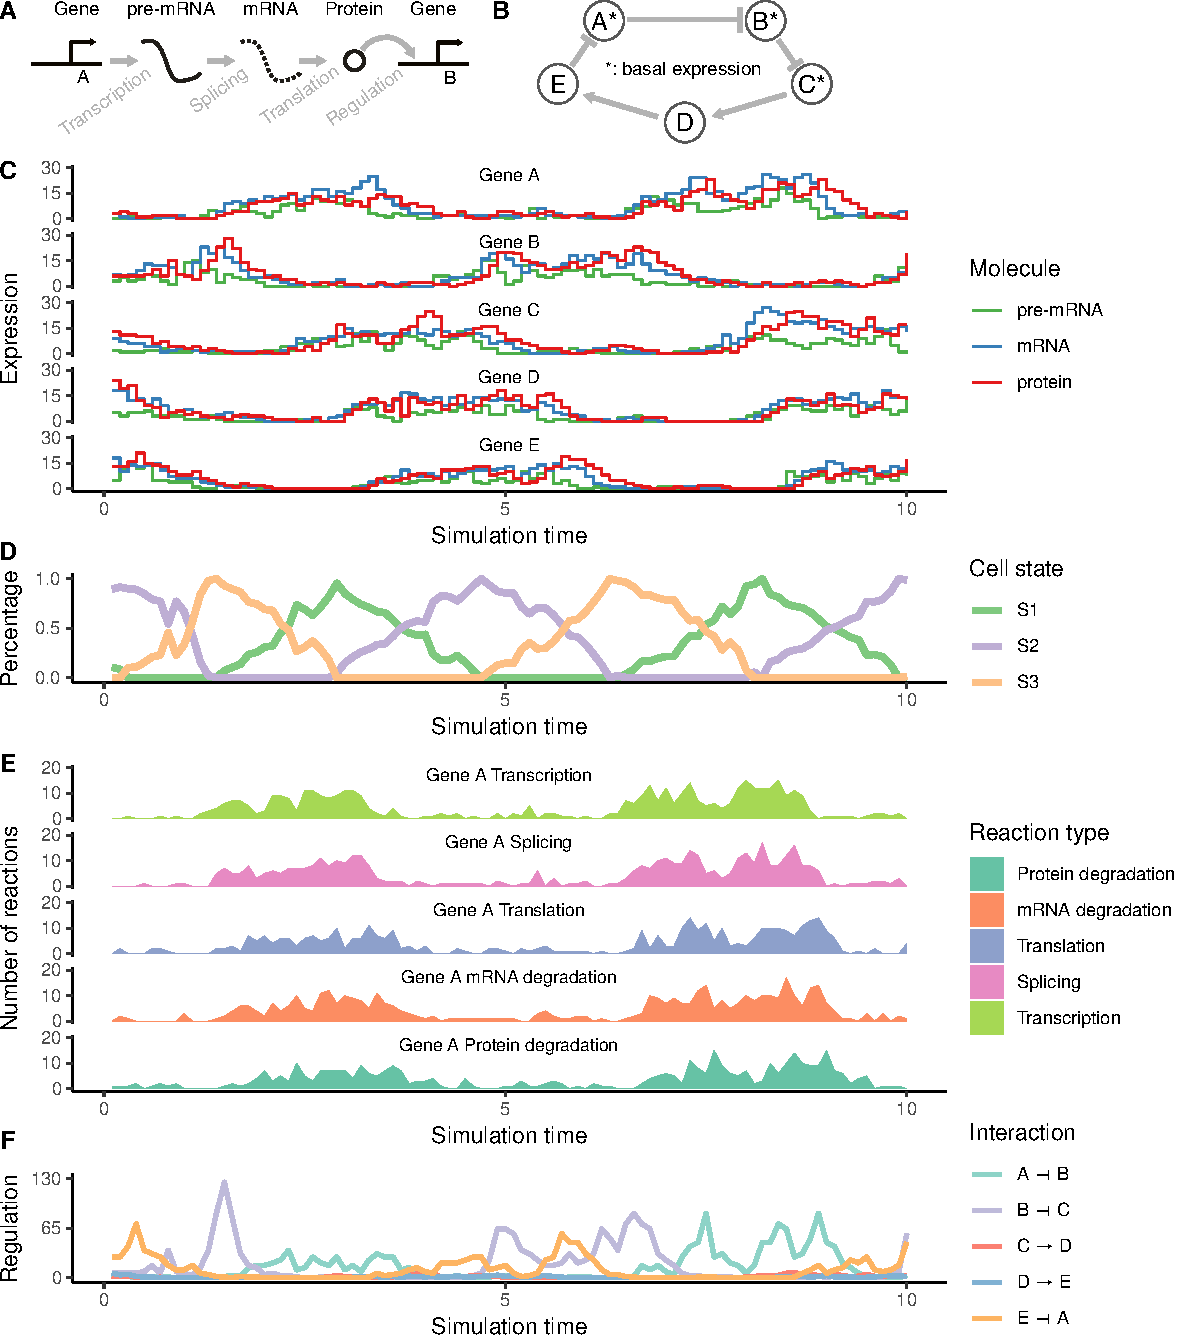
\includegraphics[width=\linewidth]{fig/simplecyclic_edited} 
	\caption{
		\textbf{Key features of \texttt{dyngen} are illustrated using a cyclic toy example.}
		While this example comprises only of a single cell and 5 genes, \texttt{dyngen} is able to simulate thousands of cells with GRNs containing thousands of genes.
	}
	\label{fig:simplecyclic}
\end{figure}

\texttt{dyngen} returns many modalities throughout the whole simulation: molecular abundance, cellular state, number of reaction firings, reaction likelihoods, and regulation activations (Figure \ref{fig:simplecyclic}C--F). These modalities can serve both as input data and ground truth for benchmarking many types of computational approaches. For example, a network inference method could use mRNA abundance and cellular states as inputs, and its output could be benchmarked against the gold standard GRN.

Depending on how the GRN is designed, different cellular developmental processes can be simulated.
\texttt{dyngen} includes generators of GRNs which result in many different developmental topologies (Figure~\ref{fig:example_runs}), including branching, converging, cyclic and even disconnected.

\begin{figure}[ht]
	\centering
	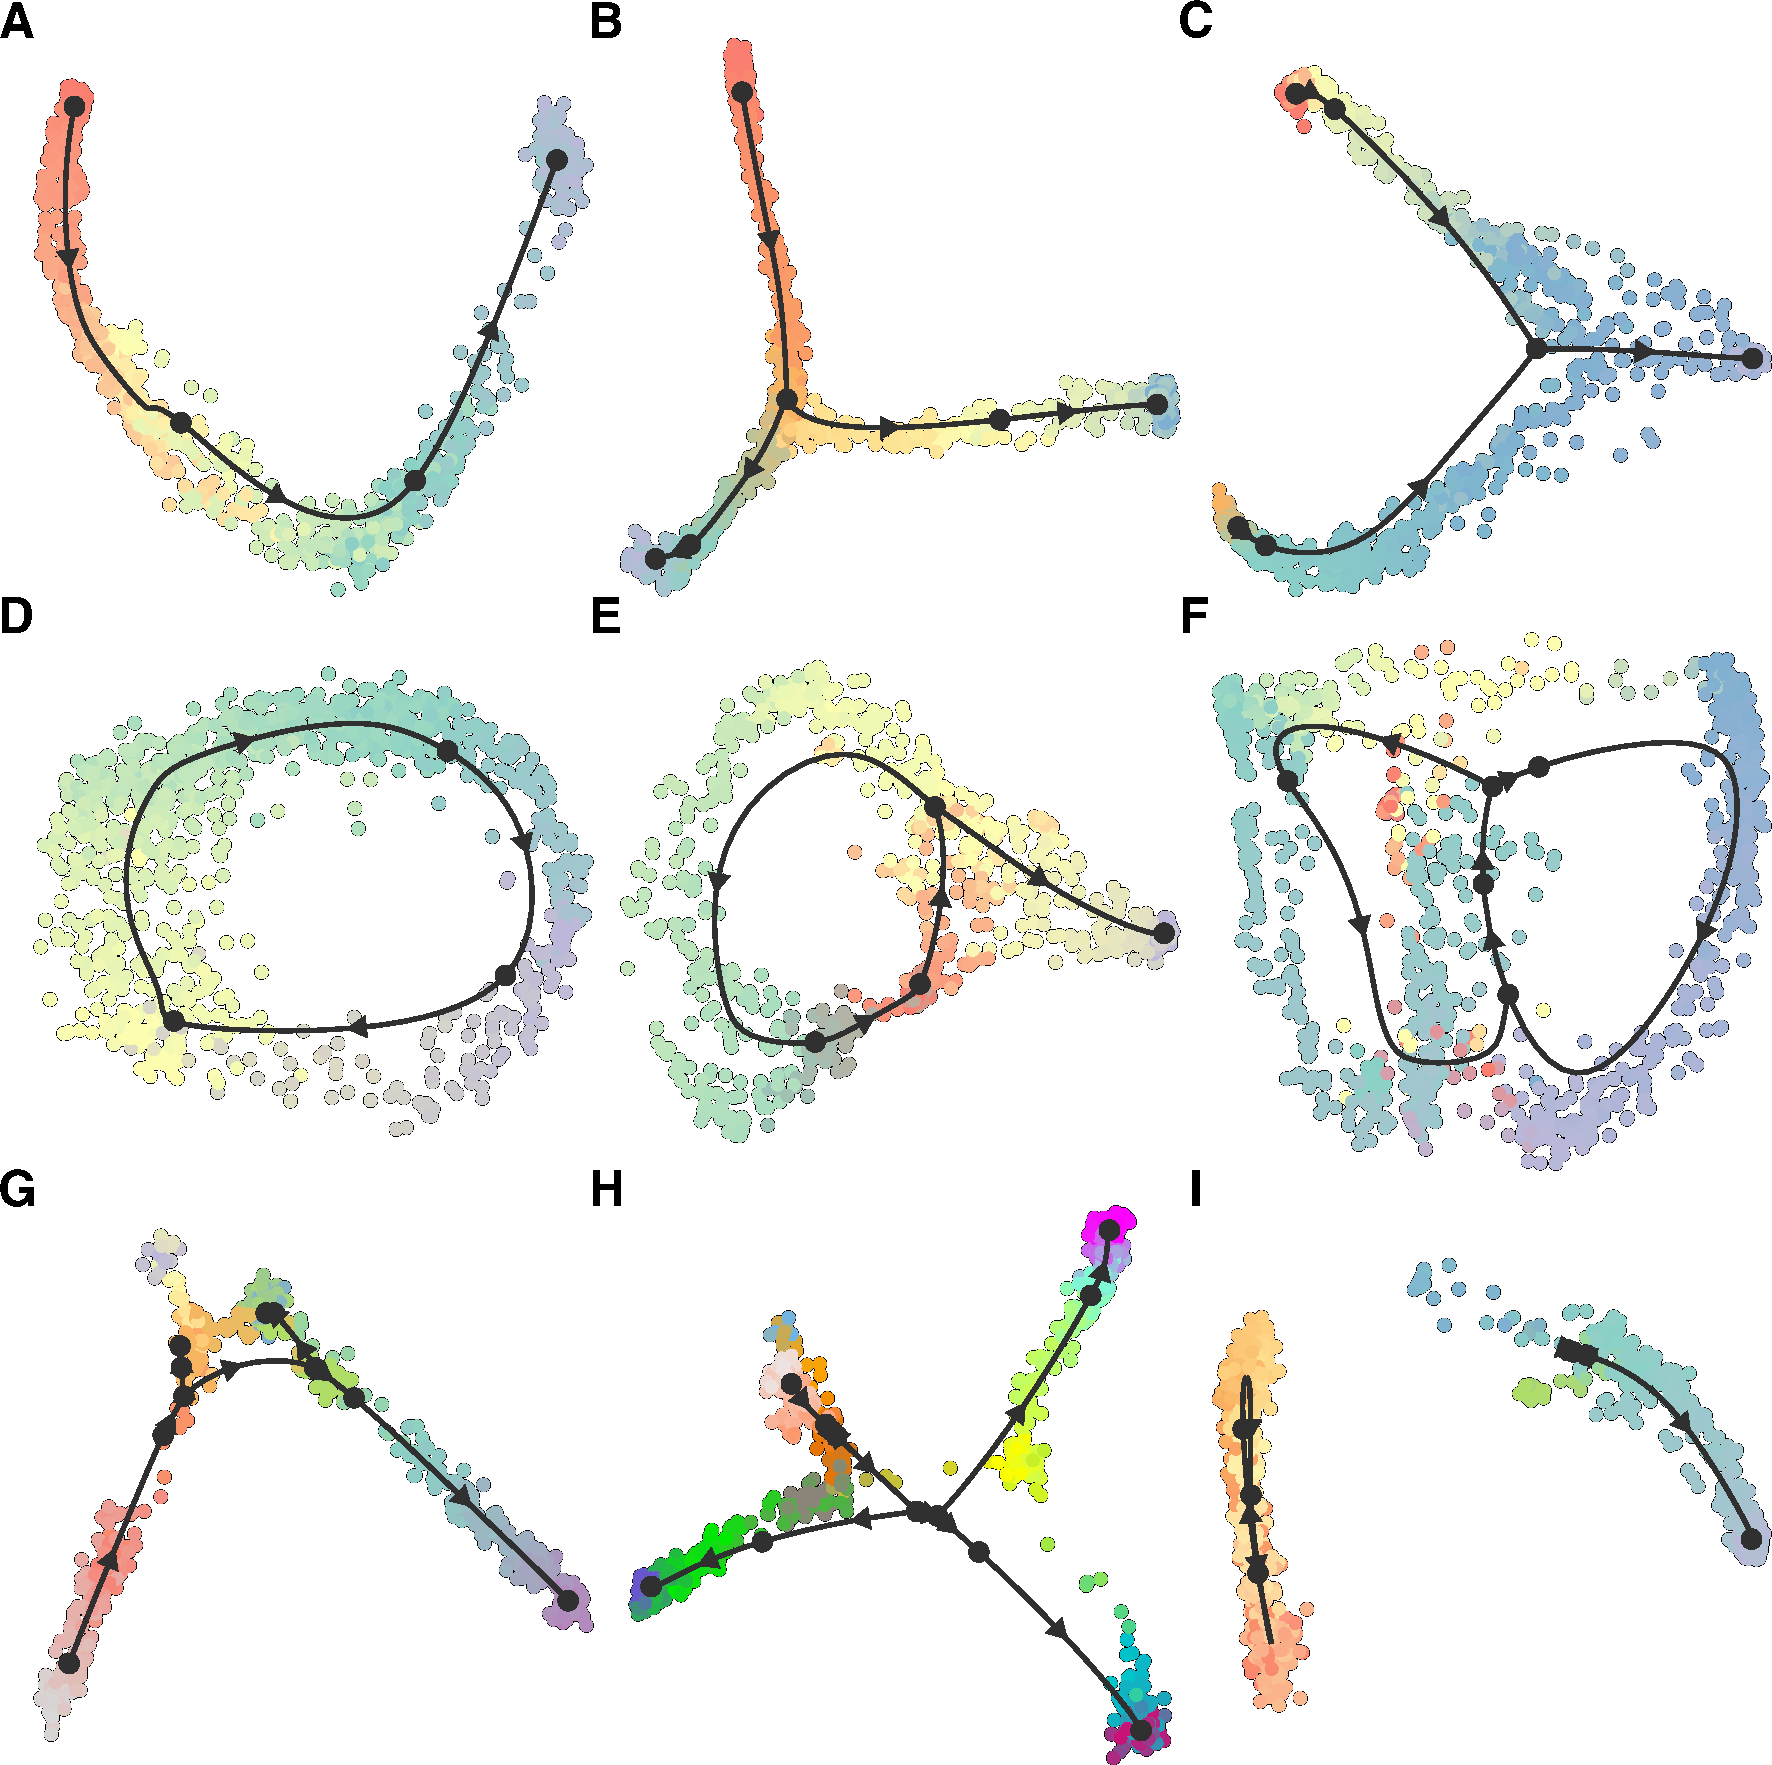
\includegraphics[width=\LARgefigure]{fig/example_runs_2} 
	\caption{
		\textbf{Multiple executions of \texttt{dyngen} with different predefined backbones.} From each simulation of about 200 genes, 1000 cells were sampled. 
		\textbf{A:}~Linear. \textbf{B:}~Bifurcating. \textbf{C:}~Converging.
		\textbf{D:}~Cyclic. \textbf{E:}~Bifurcating loop. \textbf{F:}~Bifurcating converging.
		\textbf{G:}~Consecutive branching. \textbf{H:}~Binary tree. \textbf{I:}~Disconnected.
	}
	\label{fig:example_runs}
\end{figure}

Custom-defined GRNs offer more fine-grained control over the simulation.
Aside from simulating topologies currently not supported by \texttt{dyngen}, this has several other important use-cases. Simulations of the same GRN with small perturbations allow to emulate batch effects or perturbation experiments (Figure~\ref{fig:usecases}). 
Simulating perturbed GRNs allow evaluating trajectory alignment methods -- which attempt to map two or more trajectories onto each other -- or differential network inference methods -- which infer differential regulatory interactions between two or more groups of profiles.


\begin{figure}[ht]
	\centering
	\includegraphics[width=\LARgefigure]{fig/usecases} 
	\caption{
		\textbf{Examples of simulations with perturbed GRNs.}  
		\textbf{A:} The cells in the top half were simulated with the same GRN as the cells on the bottom half, except that all parameters (e.g. strength of the interaction) were randomised.
		\textbf{B:} Only 10 interactions in the GRN were randomised. In this example, the effect of the GRN perturbation is more subtle.
	}
	\label{fig:usecases}
\end{figure}

\texttt{dyngen} can be used to simulate different experimental conditions. By default, \texttt{dyngen} supports snapshot experiments (uniformly sampling from an asynchronous dynamic process) and time-series experiments (sampling cells from different intervals in the simulation). 
However, it is possible to imagine and implement other sampling strategies, such as sampling a cell at a certain time point and once more at a later time point. This would allow evaluating the performance of RNA velocity approaches -- which predict the future state of a cell by looking at differences in pre-mRNA and mRNA abundance levels.

% YSA: RNA velocity: Onduidelijk hier, mensen kennen dit niet.


%\subsection{Example use cases}
%\subsubsection{Trajectory alignment}
%\subsubsection{Differential network inference}
%\subsubsection{RNA velocity}
%\subsubsection{Perturbation experiment}

\section{Discussion}
As is, \texttt{dyngen}'s single cell simulations can be used to evaluate common single-cell omics computational methods such as clustering, batch correction, trajectory inference and network inference.
However, the combined effect of these advantages results in a framework that is flexible enough to adapt to a broad range of applications. This may include methods that integrate clustering, network inference and trajectory inference. In this respect, \texttt{dyngen} may promote the development of new tools in the single-cell field similarly as other simulators have done in the past \cite{schaffter_genenetweaversilicobenchmark_2011,ewing_combiningtumorgenome_2015}.

\texttt{dyngen} ultimately allows anticipating technological developments in single-cell multi-omics. In this way, it is possible to design and evaluate the performance and robustness of new types of computational analyses before experimental data becomes available.
In addition, it could also be used to compare which experimental protocol is the most cost-effective in producing the qualitative and robust results in downstream analysis.

Currently, \texttt{dyngen} focuses on simulating cells as standalone entities that are well mixed.
Splitting up the simulation space into separate subvolumes could pave the way to better study key cellular processes such as cell division, intercellular communication and migration \cite{smith_spatialstochasticintracellular_2019}.


% We developed \texttt{dyngen}, a simulator of single cells to benchmark and stress-test computational tools for single-cell omics.
%It supports a selection of existing experimental protocols, but can also simulate experiments for permitted by current technologies, such as generating omics profiles from the same cell at multiple timepoints.
%This data can help kick-start emerging domains with low data availability more safely by allowing method developers to test their method before numerous datasets become publicly available.
%\texttt{dyngen} has already been used successfully to evaluate trajectory inference \cite{saelens_comparisonsinglecelltrajectory_2019}, trajectory alignment \cite{vandenberge_trajectorybaseddifferentialexpression_2019}, and network inference \cite{pratapa_benchmarkingalgorithmsgene_2019} methods. Furthermore, we showed that it can also be used to evaluate differential network inference methods, and trajectory alignment methods. % TODO: And RNA velocity?



\section{Methods}
The workflow to generate \textit{in silico} single cell data consists of six main steps (Figure \ref{fig:explain_methods}). 

\begin{figure}[htb!]
	\centering
	\includegraphics[width=\hugefigure]{fig/explain_methods} 
	\caption{\textbf{The workflow of \texttt{dyngen} is comprised of six main steps.} \textbf{A:} The user needs to specify the desired module network or use a predefined module network. \textbf{B:} Each gene in a module is is regulated by one or more transcription factors from the upstream module. Additional target genes are generated. \textbf{C:} Each gene regulatory interaction in the GRN is converted to a set of biochemical reactions. \textbf{D:} Along with the module network, the user also needs to specify the backbone structure of expected cell states. The average expression of each edge in the backbone is simulated by activating a restricted set of genes for each edge. \textbf{E:} Multiple Gillespie SSA simulations are run using the reactions defined in step C.  The counts of each of the molecules at each time step are extracted. Each time step is mapped to a point in the backbone. \textbf{F:} Multiple cells are sampled from each simulation. Molecules are sampled from each cell.}
	\label{fig:explain_methods}
\end{figure}

\subsection{Defining the backbone: modules and states} \label{sec:backbone}

One of the main processes involved in cellular dynamic processes is gene regulation, where regulatory cascades and feedback loops lead to progressive changes in expression and decision making. The exact way a cell chooses a certain path during its differentiation is still an active research field, although certain models have already emerged and been tested \textit{in vivo}. One driver of bifurcation seems to be mutual antagonism, where two genes strongly repress each other \cite{rekhtman_directinteractionhematopoietic_1999,xu_regulationbifurcatingcell_2015}, forcing one of the two to become inactive \cite{graf_forcingcellschange_2009}. Such mutual antagonism can be modelled and simulated \cite{wang_quantifyingwaddingtonlandscape_2011, ferrell_bistabilitybifurcationswaddington_2012}. Although the two-gene model is simple and elegant, the reality is frequently more complex, with multiple genes (grouped into modules) repressing each other \cite{yosef_dynamicregulatorynetwork_2013}.

In \texttt{dyngen}, the user defines the behaviour of the simulation by defining how sets of genes, called modules, are regulating eachother.
A module may have basal expression, which means that pre-mRNA of the genes in this module will be transcribed without the presence of transcription factor molecules. A module marked as "active during the burn phase" means that this module will be allowed to generate expression of its genes during an initial warm-up phase (See section \ref{sec:dyngen_ssa}). At the end of the \texttt{dyngen} process, cells will not be sampled from the burn phase simulations. Interactions between modules have a strength (which is a positive integer) and an effect (+1 for upregulating, -1 for downregulating).

Several examples of module networks are given (Figure \ref{fig:example_backbones}). 
A simple chain of modules (where one module upregulates the next) results in a \emph{linear} process. By having the last module repress the first module, the process becomes \emph{cyclic}. Two modules repressing eachother is the basis of a \emph{bifurcating} process, though several chains of modules have to be attached in order to achieve progression before and after the bifurcation process. Finally, a \emph{converging} process has a bifurcation occurring during the burn phase, after which any differences in module regulation is removed.

Note that these examples represent the bare minimum in terms of number of modules used. Using longer chains of modules is typically desired. In addition, the fate decisions made in this example of a bifurcation is reversible, meaning cells can be reprogrammed to go down a different differentiation path. If this effect is undesirable, more safeguards need to be put in place to prevent reprogramming from occurring (Section \ref{sec:dyngen_backbone_lego}).

\begin{figure}[htb!]
	\centering
	\includegraphics[width=\LARGEfigure]{fig/example_backbones} 
	\caption{Example module networks}
	\label{fig:example_backbones}
\end{figure}

In addition to the module network, the user also needs to define a network of cellular states called the "backbone". Before simulating any cells, each transition in the backbone is simulated separately to obtain the average changes in expression along that transition (Figure \ref{fig:explain_methods}D). As part of the backbone, the user needs to specify which modules are allowed to alter its expression from one state to another. For example, in order to transition from state S0 to S1 in the cyclic example, gene modules A, B and C are turned on and a simulation is allowed to run. To transition from S1 to S2, gene modules D and E are turned on, and expression of gene module C is kept constant. To transition from S2 to S3, C is turned on again and now A and B are fixed. Finally, to transition from S3 to S1 again, A and B are turned on again and D and E are fixed again. Demonstrations of the backbone will be explained in more detail in section \ref{sec:dyngen_sim_backbone}.

\subsubsection{Backbone lego} \label{sec:dyngen_backbone_lego}
The backbone can make use of one or more "backbone lego" (BBL) pieces (Figure \ref{fig:backbone_lego}). A BBL consists of one or more modules which regulate each other such that the output modules present a specific behaviour, depending on the input module (Figure \ref{fig:backbone_lego}A). Parameters allow determining the number of modules involved in the process and the number of outputs. Multiple BBLs can be chained together in order to intuitively create milestone networks and corresponding state networks (Figure \ref{fig:backbone_lego}B). Note that not all dynamic processes can be represented by a combination of BBLs, but they can serve as common building blocks to aid the construction of the backbone.

\begin{figure}[htb!]
	\centering
	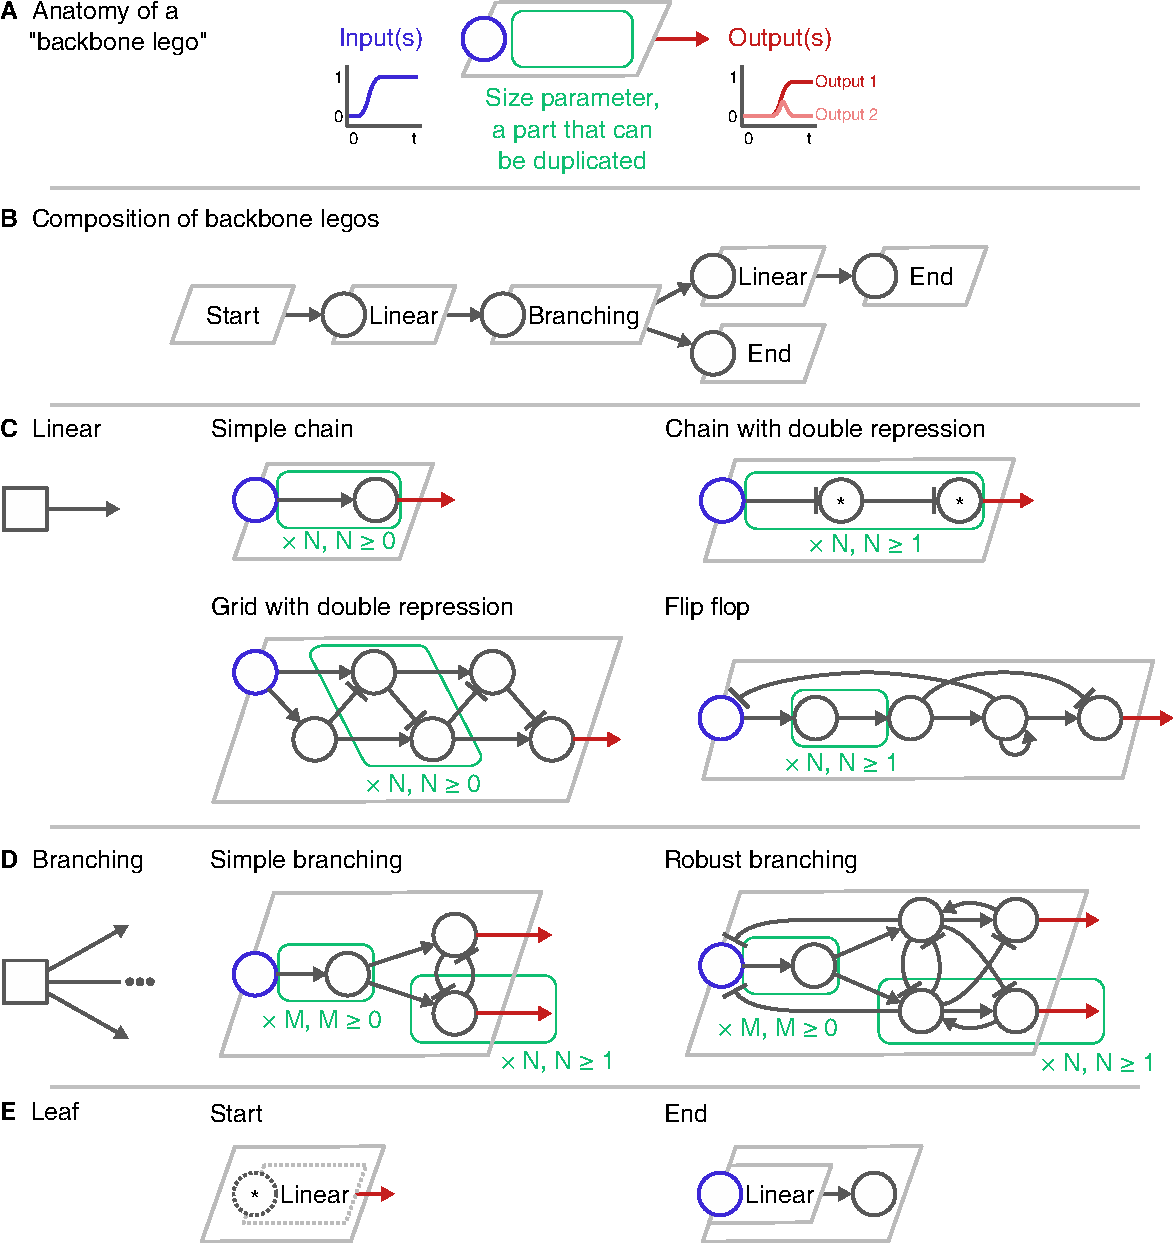
\includegraphics[width=\LARGEfigure]{fig/backbone_lego} 
	\caption{Backbone lego}
	\label{fig:backbone_lego}
\end{figure}

When the input node of a \textbf{linear BBL} (Figure \ref{fig:backbone_lego}C) is upregulated, the module the BBL is connected to will be upregulated. A \emph{simple chain} is a set of modules where a module upregulates the next. A \emph{chain with double repression} has an uneven number of modules forming a chain where each module downregulates the next but all modules (except the input) have basal expression. A \emph{grid with double repression} is similar; except that modules do not have basal expression but instead get upregulated by an upstream module in the chain. Finally, a \emph{flip flop} consists of a simple chain where first the modules (except the last) are upregulated. Once the second to last module is upregulated, that module upregulates itself and the first module is strongly repressed, causing all other modules to lose expression and finally the last module to be upregulated. The \emph{flip flop} retains this output state, even when the input changes.

When the input node of a \textbf{branching BBL} (Figure \ref{fig:backbone_lego}D) is upregulated, a subset of its output modules will eventually be upregulated. A \emph{simple branching} uses reciprocal inhibition to drive the upregulation of one of the output modules. Due to its simplicity, however, multiple output modules might be upregulated simultaneously, and over long periods of simulation time it might be possible that the choice of upregulated module changes. A \emph{robust branching} improves upon the simple branching by preventing upregulation of output modules until an internal branching decision has been made, and by repressing the decision mechanism to avoid other output modules being upregulated other than the one that has been chosen.

A \textbf{leaf BBL} (Figure \ref{fig:backbone_lego}E) is a linear BBL that has either no inputs or no outputs. A \emph{start} BBL is a linear BBL where the first module has basal expression, and all modules in this module will be active during the burn-in phase of the simulation (Section \ref{sec:dyngen_sim_backbone}). An \emph{end} BBL is also a linear BBL with its output regulating one final module. 


\subsection{Generating the gene regulatory network}
The GRN is generated based on the given backbome in four main steps (Figure~\ref{fig:gen_feature_network}).

\begin{figure}[htb!]
	\centering
	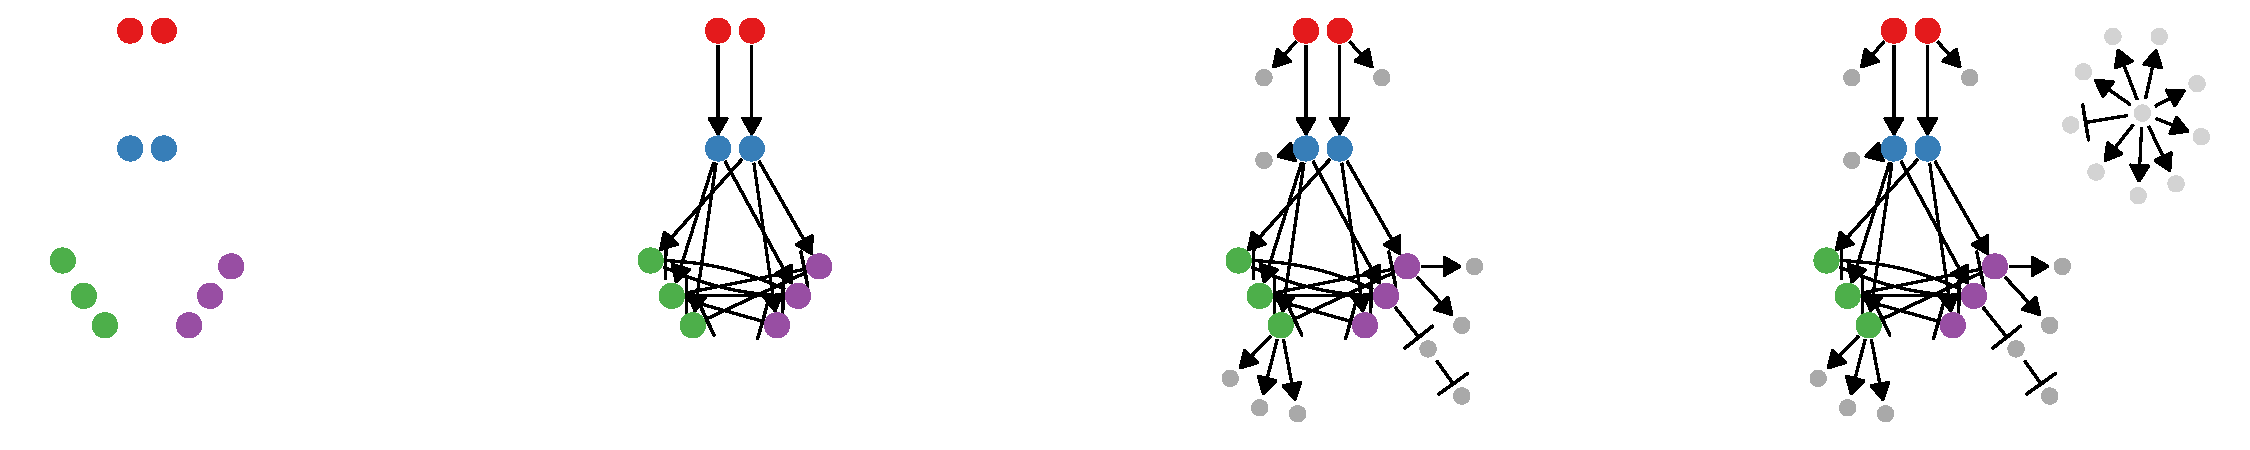
\includegraphics[width=\linewidth]{fig/gen_feature_network} 
	\caption{
		\textbf{Generating the feature network from a backbone consists of four main steps.}
	}
	\label{fig:gen_feature_network}
\end{figure}

\paragraph{Step 1, sampling the transcription factors (TF).} The TFs are the main drivers of the molecular changes in the simulation. The user provides a backbone and the number of TFs to generate. Each TF is assigned to a module such that each module has at least $x$ parameters (default $x=1$). A TF inherits the 'burn' and 'basal expression' from the module in belongs to.

\paragraph{Step 2, generating the TF interactions.} Let each TF be regulated according to the interactions in the backbone. These interactions inherit the effect, strength, and cooperativity parameters from the interactions in the backbone. A TF can only be regulated by other TFs or itself.

\paragraph{Step 3, sampling the target subnetwork.} 
A user-defined number of target genes are added to the GRN. Target genes regulated by a TF or another target gene, but is always downstream of at least one TF. To sample the interactions between target genes, one of the many FANTOM5 \cite{lizio_gatewaysfantom5promoter_2015} GRNs is sampled. The currently existing TFs are mapped to regulators in the FANTOM5 GRN. The targets are drawn from the FANTOM5 GRN, weighted by their page rank value. For each target, at most $x$ regulators are sampled from the induced FANTOM5 GRN (default $x=5$). The interactions connecting a target gene and its regulators are added the GRN.


\paragraph{Step 4, sampling the housekeeping subnetwork.}
Housekeeping genes are completely separate from any TFs or target genes. A user-defined set of housekeeping genes are also sampled from the FANTOM5 GRN. The interactions of the FANTOM5 GRN are first subsampled such that the maximum in-degree of each gene is $x$ (default $x=5$). A random gene is sampled, and a breadth-first-search is performed to sample the desired number of housekeeping genes.

\subsection{Convert gene regulatory network to a set of reactions} \label{sec:reactions}
% paper on transcriptional bursting
% doi: 10.1039/C7MB00154A
% interesting to try to replicate in dyngen! :)
\newcommand{\w}[1]{\text{w}_{#1}}
\newcommand{\x}[1]{\text{x}_{#1}}
\newcommand{\y}[1]{\text{y}_{#1}}


\newcommand{\rs}[1]{\text{R}_{#1}}
\newcommand{\rp}[1]{\text{R}^+_{#1}}
\newcommand{\rn}[1]{\text{R}^-_{#1}}

\newcommand{\wpr}[1]{\text{wpr}_{#1}}
\newcommand{\wsr}[1]{\text{wsr}_{#1}}
\newcommand{\xdr}[1]{\text{xdr}_{#1}}
\newcommand{\ypr}[1]{\text{ypr}_{#1}}
\newcommand{\ydr}[1]{\text{ydr}_{#1}}

\newcommand{\str}[1]{\text{str}_{#1}}
\newcommand{\co}[1]{\text{co}_{#1}}
\newcommand{\ind}[1]{\text{ind}_{#1}}
\newcommand{\hmy}[1]{\text{hmy}_{#1}}
\newcommand{\reg}[1]{\text{reg}_{#1}}
\newcommand{\ba}[1]{\text{ba}_{#1}}

For every gene $G$ in the GRN, the simulation will keep track of the abundance levels of three molecules, a pre-mRNA, a mature mRNA and a protein. These abundance levels are represented as $\w G$, $\x G$ and $\y G$ respectively. 

Throughout a simulation, the abundance levels of molecules are affected by five reactions, namely transcription, splicing, mRNA degradation, translation, and protein degradation. Each reaction consists of its propensity -- a formula to calculate the probability of the reaction occurring during an infinitesimal time interval -- and the effect -- how it will affect the current state if triggered. The effects and propensity functions of these reactions are defined in Table \ref{tab:reaction_def}.


%!!!!!!!!!!!!!!!!!!!!!!!!!!!!!!!!!!!!!!!!!!!!!!!!!!!!!!!!!!!!!!!
% TODO: add step-by-step  derivation of transcription formula
%!!!!!!!!!!!!!!!!!!!!!!!!!!!!!!!!!!!!!!!!!!!!!!!!!!!!!!!!!!!!!!!

% YSA: Graag wat meer uitleg in de tekst over al deze formules, definitie van notaties en zo.

\begin{table}[ht]
	\caption{\textbf{Reactions affecting the abundance levels of pre-mRNA $\w G$, mRNA $\x G$ and proteins $\y G$ of gene $G$.} Define the set of regulators of $G$ as $\rs{G}$, the set of upregulating regulators of $G$ as $\rp G$, and the set of downregulating regulators of $G$ as $\rn G$. Parameters used in the propensity formulae are defined in Table \ref{tab:reaction_params}.} \label{tab:reaction_def}
	\centering
	\begin{tabular}{|lcc|}
		\hline
		Reaction & Effect & Propensity \\ \hline \hline
		Transcription & $\emptyset \rightarrow \w G$ & $\wpr G \times \frac{\ba G - \ind{G}^{|\rp{G}|} + \prod\limits_{H \in \rp{G}}(\ind G + \reg{G,H})}{\prod\limits_{H \in \rs{G}}(1 + \reg{G,H})}$ \\
		Splicing & $\w G \rightarrow \x G$ & $\wsr G \times \w G$ \\
		mRNA degradation & $\x G \rightarrow \emptyset$ & $\xdr G \times \x G$ \\
		Translation & $\x G \rightarrow \w G + \y G$ & $\ypr G \times \x G$ \\
		Protein degradation & $\y G \rightarrow \emptyset$ & $\ydr G \times \y G$ \\ \hline
	\end{tabular}
\end{table}

% regG,H represents a 'probability' that H is bound to G (though does not yet scale between [0,1]). y_H / maxy_H is more likely to be a probability that H is bound to G, though this does not take into account that H can be bound to other genes as well. 
% in any case, if it is, then it upregulates G by strG,H. It is assumed binding events
% are independent and result in multiplicative effect.

% according to https://en.wikipedia.org/wiki/Hill_equation_(biochemistry)#Proportion_of_ligand-bound_receptors:
% P_H = (y_H ^ N) / (degradation_H / production_H + y_H ^ N)
% ... 
% ... 
% might need to go back to things like:
% https://kar.kent.ac.uk/24077/1/myzabetpaper.pdf

\begin{table}[ht]
	\caption{\textbf{Default parameters defined for the calculation of reaction propensity functions.}} \label{tab:reaction_params}
	\centering
	\begin{tabular}{|lrl|}
		\hline
		Parameter & Symbol & Definition \\ \hline \hline
		Transcription rate & $\wpr{G}$ & $\in N(100, 20),\ \geq 10$ \\
		Splicing rate & $\wsr G$ & $\in N(10, 2),\ \geq 2$ \\
		mRNA degradation rate & $\xdr{G}$ & $\in N(5, 1),\ \geq 2$ \\
		Translation rate & $\ypr{G}$ & $\in N(5, 1),\ \geq 2$ \\
		Protein degradation rate & $\ydr G$ & $\in N(3, 0.5),\ \geq 1$ \\
		Interaction strength & $\str{G,H}$ & $\in 10^{U(0, 2)}$ * \\ 
		Interaction cooperativity & $\co{G,H}$ & $\in U(0.5, 2)$ * \\
    Independence factor & $\ind G$ & $\in [0, 1]$ * \\ \hline\hline
		TF concentration at half-maximal binding & $\hmy H$ & $= 0.5 \times \frac{\wpr H \times \ypr H}{\xdr H \times \ydr H}$ \\ 
		Regulation activity & $\reg{G,H}$ & $= \left(\str{G,H} \times \frac{\y H}{\hmy H}\right) ^ {\co{G,H}}$ \\
		Basal expression & $\ba G$ & $= \begin{cases} 1 & \mbox{if } \rp{G} = \emptyset \\ 0.0001 & \mbox{if } \rn{G} = \emptyset \mbox{ and } \rp{G} \neq \emptyset \\ 0.5 & \mbox{otherwise} \end{cases}$ * \\ \hline
		\multicolumn{3}{l}{*: unless $G$ is a TF, then the value is determined by the backbone.}
	\end{tabular}
\end{table}

\subsection{Compute average expression along backbone transitions} \label{sec:dyngen_sim_backbone}
When simulating the developmental backbone, we go through the edges of the backbone state network defined in an earlier step (Section \ref{sec:backbone}), starting from the root state. It is assumed the root state has no modules active and has no expression of any molecules. To get to the next state, we follow a transition starting from the root state, activate and deactivate the modules as indicated by the transition, and compute the average molecule abundance along the transition. To compute the average abundance, we perform small time steps $t = 0.001$ and let each reaction (Section \ref{sec:reactions}) occur $t$ times its propensity. 

% mention that this is basically an ode?

\subsection{Simulate single cells} \label{sec:dyngen_ssa}
%TODO: STOCKS \cite{kierzek_stocksstochastickinetic_2002} uses GSSA to simulate something.
% maybe we could have a look at that! 
% or https://nyaspubs.onlinelibrary.wiley.com/doi/full/10.1111/j.1749-6632.2008.03756.x

% or even https://academic.oup.com/bioinformatics/article/24/10/1318/178687 ('AND' and 'OR')
% and https://academic.oup.com/bioinformatics/article/25/9/1205/203870 (regulation motifs, kinetics)
% https://nyaspubs.onlinelibrary.wiley.com/doi/full/10.1111/j.1749-6632.2008.03756.x (modules of genes)

%TODO: improve this section a lot. Basically, explain SSA and GillespieSSA2.


\texttt{dyngen} uses Gillespie's stochastic simulation algorithm (SSA) \cite{gillespie_exactstochasticsimulation_1977} to simulate dynamic processes. An SSA simulation is an iterative process where at each iteration one reaction is triggered. 

Each reaction consists of its propensity -- a formula to calculate the probability of the reaction occurring during an infinitesimal time interval -- and the effect -- how it will affect the current state if triggered. Each time a reaction is triggered, the simulation time is incremented by $\tau = \frac{1}{\sum_j prop_j} \ln\left(\frac{1}{r}\right)$, with $r \in U(0, 1)$ and $prop_j$ the propensity value of the $j$th reaction for the current state of the simulation.

\texttt{GillespieSSA2} is an optimised library for performing SSA simulations. The propensity functions are compiled to C++, and SSA approximations can be used which allow to trigger many reactions simultaneously at each iteration. The framework also allows to store the abundance levels of molecules only after a specific interval has passed since the previous census. By setting the census interval to 0, the whole simulation's trajectory is retained but many of these time points will contain very similar information. In addition to the abundance levels, also the propensity values and the number of firings of each of the reactions at each of the time steps can be retained, as well as specific sub-calculations of the propensity values, such as the regulator activity level $reg_{G,H}$. 

\subsubsection{Map SSA simulations to backbone}
We compute the Pearson correlation between the state vectors in the simulation and the average expression levels along a transition in the backbone. Each timepoint in the SSA simulation is mapped to the point in the backbone that has the highest correlation value.

\subsection{Simulate experiment}
From the SSA simulation we obtain the abundance levels of all the molecules at the different time points. We need to replicate technical effects introduced by experimental protocols in order to obtain data that is similar to real data. For this, the cells are sampled from the simulations, and molecules are sampled for each of the cells. Real datasets are used in order to achieve similar data characteristics.

\subsubsection{Sample cells}
Cells can be sampled from an unsynchronised population of single cells (snapshot) or at multiple time points in a synchronised population (time series).

\paragraph{Snapshot} Cells are sampled uniformly from the different time points in the simulation.

\paragraph{Time series} The timeline of the simulations is divided into multiple chunks. From several of these chunks, cells are sampled. For each cell it is known at which time point it was sampled.

\subsubsection{Sample molecules} 
Molecules are sampled from the simulation to replicate how molecules are experimentally sampled. A real dataset is downloaded from a repository of single-cell RNA-seq datasets \cite{cannoodt_singlecellomicsdatasets_2018}. For each \textit{in silico} cell $i$, draw its library size $ls_i$from the distribution of transcript counts per cell in the real dataset. The capture rate $cr_j$ of each \textit{in silico} molecule type $j$ is drawn from $N(1, 0.05)$. Finally, for each cell $i$, draw $ls_i$ molecules from the multinomial distribution with probabilities $cr_j \times ab_{i,j}$ with $ab_{i,j}$ the molecule abundance level of molecule $j$ in cell $i$.


\clearpage
\section{References}
\printbibliography[heading=none]


%%%%%%%%%%%%%%%%%%%%%%%%%%%%%%%%%
%%%     CH3: DYNBENCHMARK     %%%
%%%%%%%%%%%%%%%%%%%%%%%%%%%%%%%%%
\newpage{\thispagestyle{empty}\cleardoublepage}
\chapter{dynbenchmark: A comparison of single-cell trajectory inference methods} 
\chaptermark{dynbenchmark: A comparison of single-cell trajectory inference methods.} % short title
\label{chap:dynbenchmark}
\graphicspath{{./ch3_dynbenchmark/}}
\begin{quote}
	\textbf{Abstract:} Trajectory inference approaches analyze genome-wide omics data from thousands of single cells and computationally infer the order of these cells along developmental trajectories. Although more than 70 trajectory inference tools have already been developed, it is challenging to compare their performance because the input they require and output models they produce vary substantially. Here, we benchmark 45 of these methods on 110 real and 229 synthetic datasets for cellular ordering, topology, scalability and usability. Our results highlight the complementarity of existing tools, and that the choice of method should depend mostly on the dataset dimensions and trajectory topology. Based on these results, we develop a set of guidelines to help users select the best method for their dataset. Our freely available data and evaluation pipeline (\href{https://benchmark.dynverse.org}{benchmark.dynverse.org}) will aid in the development of improved tools designed to analyze increasingly large and complex single-cell datasets.
\end{quote}
\vfill
Adapted from:\\
Saelens, W.$^*$, \textbf{Cannoodt, R.}$^*$, Todorov, H., and Saeys, Y. A comparison of single-cell trajectory inference methods. \textit{Nature Biotechnology} 37, 5 (2019), 547--554. \doi{10.1038/s41587-019-0071-9}.\\
{\footnotesize $^*$ Equal contribution}
\newpage
\section{Introduction}
Single-cell omics data, including transcriptomics, proteomics and epigenomics data, provide new opportunities for studying cellular dynamic processes, such as the cell cycle, cell differentiation and cell activation \cite{tanay_scalingsinglecellgenomics_2017,etzrodt_quantitativesinglecellapproaches_2014}. Such dynamic processes can be modelled computationally using trajectory inference (TI) methods, also called pseudotime analysis, which order cells along a trajectory based on similarities in their expression patterns \cite{trapnell_definingcelltypes_2015,cannoodt_computationalmethodstrajectory_2016,moon_manifoldlearningbasedmethods_2018}. The resulting trajectories are most often linear, bifurcating or tree-shaped, but more recent methods also identify more complex trajectory topologies, such as cyclic \cite{liu_reconstructingcellcycle_2017} or disconnected graphs \cite{wolf_graphabstractionreconciles_2017}. TI methods offer an unbiased and transcriptome-wide understanding of a dynamic process \cite{tanay_scalingsinglecellgenomics_2017}, thereby allowing the objective identification of new (primed) subsets of cells \cite{schlitzer_identificationcdc1cdc2committed_2015}, delineation of a differentiation tree \cite{velten_humanhaematopoieticstem_2017,see_mappinghumandc_2017} and inference of regulatory interactions responsible for one or more bifurcations \cite{aibar_scenicsinglecellregulatory_2017}. Current applications of TI focus on specific subsets of cells, but ongoing efforts to construct transcriptomic catalogues of whole organisms \cite{regev_humancellatlas_2017,han_mappingmousecell_2018,schaum_singlecelltranscriptomics20_2018} underline the urgency for accurate, scalable \cite{aibar_scenicsinglecellregulatory_2017,angerer_singlecellsmake_2017} and user-friendly TI methods.

A plethora of TI methods has been developed over the past few years and even more are being created every month (Supplementary Table~\hyperref[tab:supptable_1]{3.1}). Indeed, in several repositories listing single-cell tools, such as omictools.org \cite{henry_omictoolsinformativedirectory_2014}, the ‘awesome-single-cell’ list \cite{davis_awesomesinglecell_2018} and scRNA-tools.org \cite{zappia_exploringsinglecellrnaseq_2017}, TI methods are one of the largest categories. While each method has its own unique set of characteristics in terms of underlying algorithm, required prior information and produced outputs, two of the most distinctive differences between TI methods are whether they fix the topology of the trajectory and what type(s) of graph topologies they can detect. Early TI methods typically fixed the topology algorithmically (for example, linear \cite{bendall_singlecelltrajectorydetection_2014,schlitzer_identificationcdc1cdc2committed_2015,shin_singlecellrnaseqwaterfall_2015,campbell_bayesiangaussianprocess_2015} or bifurcating trajectories \cite{haghverdi_diffusionpseudotimerobustly_2016,setty_wishboneidentifiesbifurcating_2016}) or through parameters provided by the user \cite{trapnell_dynamicsregulatorscell_2014,matsumoto_scoupprobabilisticmodel_2016}. These methods therefore mainly focus on correctly ordering the cells along the fixed topology. More recent methods also infer the topology \cite{qiu_reversedgraphembedding_2017,street_slingshotcelllineage_2018,wolf_graphabstractionreconciles_2017}, which increases the difficulty of the problem at hand, but allows the unbiased identification of both the ordering inside a branch and the topology connecting these branches.

Given the diversity in TI methods, it is important to quantitatively assess their performance, scalability, robustness and usability. Many attempts at tackling this issue have already been made \cite{haghverdi_diffusionpseudotimerobustly_2016,ji_tscanpseudotimereconstruction_2016,welch_slicerinferringbranched_2016,matsumoto_scoupprobabilisticmodel_2016,duverle_celltreebioconductorpackage_2016,cannoodt_computationalmethodstrajectory_2016,lonnberg_singlecellrnaseqcomputational_2017,campbell_probabilisticmodelingbifurcations_2017,wolf_graphabstractionreconciles_2017}, but a comprehensive comparison of TI methods across a large number of different datasets is still lacking. This is problematic, as new users to the field are confronted with an overwhelming choice of TI methods, without a clear idea of which would optimally solve their problem. Moreover, the strengths and weaknesses of existing methods need to be assessed, so that new developments in the field can focus on improving the current state-of-the-art.

In this study, we evaluated the accuracy, scalability, stability and usability of 45 TI methods (Figure \ref{fig:figure_1}a). We found substantial complementarity between current methods, with different sets of methods performing most optimally depending on the characteristics of the data. For method users, we created an interactive set of guidelines (available at \url{http://guidelines.dynverse.org}), which gives context-specific recommendations for method usage. Our evaluation also highlights some challenges for current methods, and our evaluation strategy can be useful to spearhead the development of new tools that accurately infer trajectories on ever more complex use cases.

\begin{figure}[tbh!]
	\centering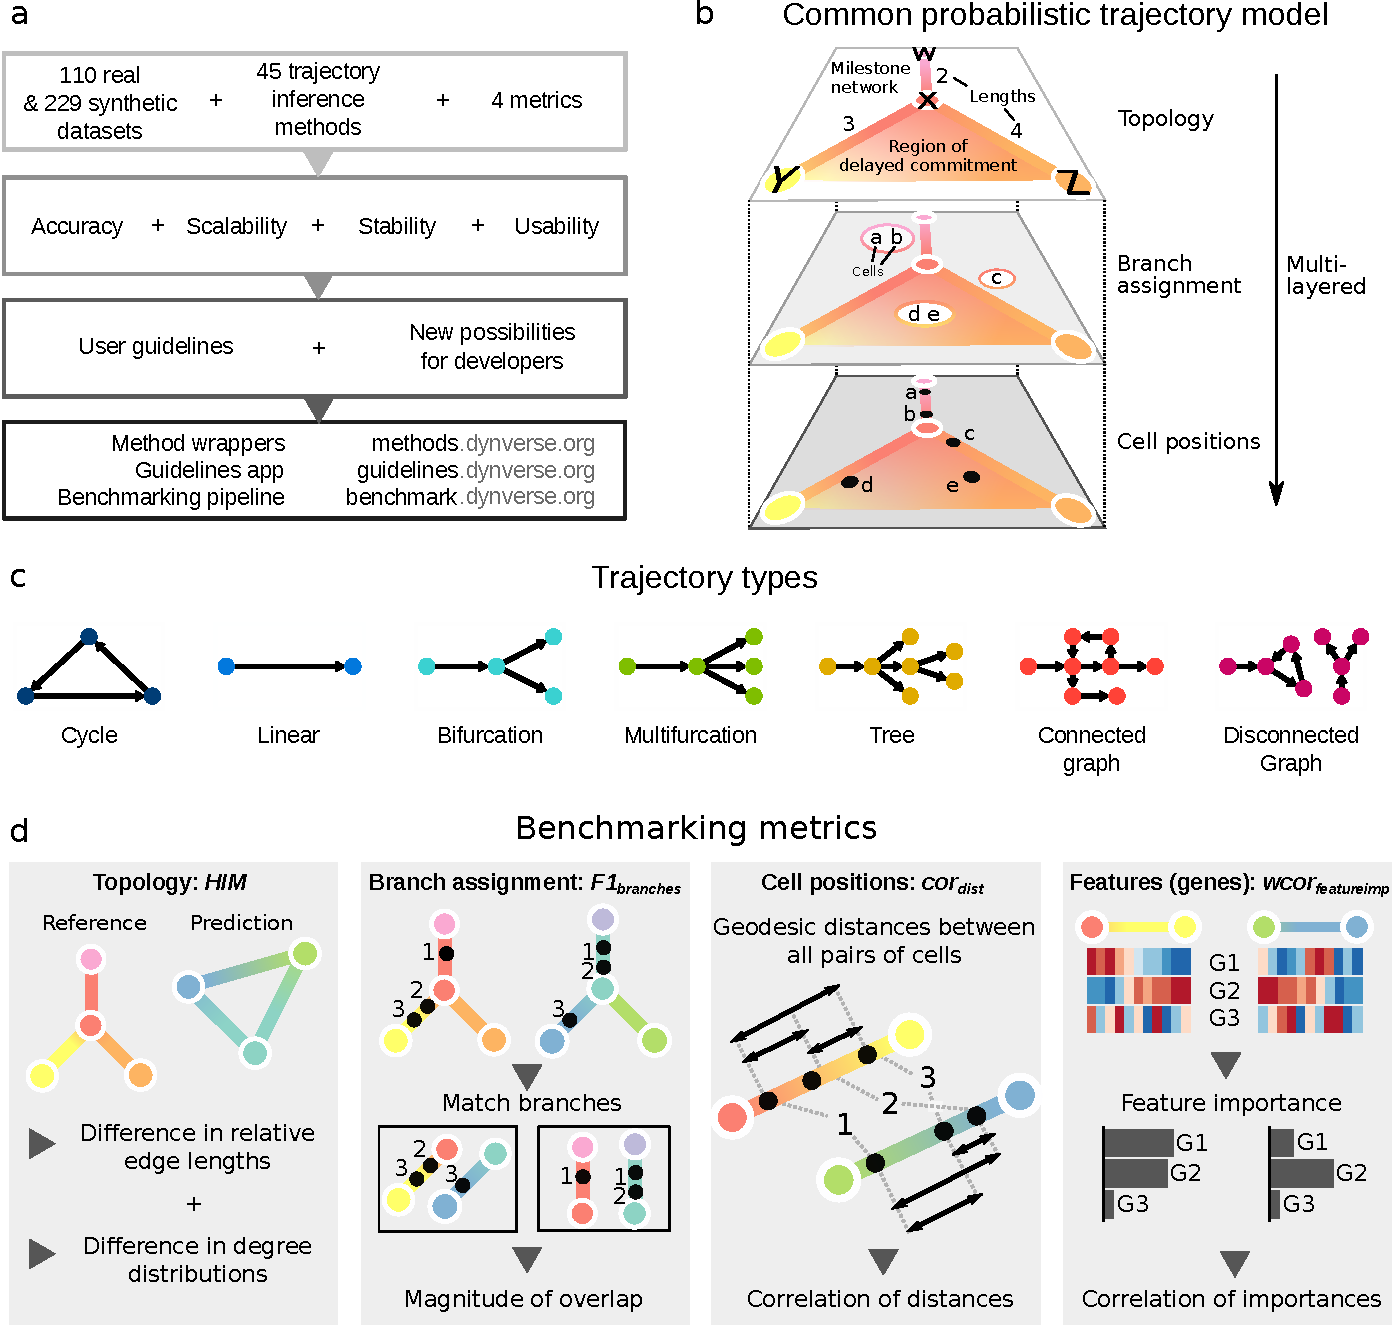
\includegraphics[width=\linewidth]{fig/figure_1.pdf}
	\caption{
		\textbf{Overview of several key aspects of the evaluation.}
		\textbf{a}, A schematic overview of our evaluation pipeline. \textbf{b}, To make the trajectories comparable to each other, a common trajectory model was used to represent reference trajectories from the real and synthetic datasets, as well as any predictions of TI methods. \textbf{c}, Trajectories are automatically classified into one of seven trajectory types, with increasing complexity. \textbf{d}, We defined four metrics, each assessing the quality of a different aspect of the trajectory. The HIM score assesses the similarity between the two topologies, taking into account differences in edge lengths and degree distributions. The F1branches assesses the similarity of the assignment of cells onto branches. The cordist quantifies the similarity in cellular positions between two trajectories, by calculating the correlation between pairwise geodesic distances. Finally, wcorfeatures quantifies the agreement between trajectory differentially expressed features from the known trajectory and the predicted trajectory.
	}
	\label{fig:figure_1}
\end{figure}


\section{Results}

\subsection{Trajectory inference methods}
To make the outputs from different methods directly comparable to each other, we developed a common probabilistic model for representing trajectories from all possible sources (Figure \ref{fig:figure_1}b). In this model, the overall topology is represented by a network of ‘milestones’, and the cells are placed within the space formed by each set of connected milestones. Although almost every method returned a unique set of outputs, we were able to classify these outputs into seven distinct groups (Figure \ref{fig:supfigure_1}) and we wrote a common output converter for each of these groups (Figure \ref{fig:figure_2}a). When strictly required, we also provided prior information to the method. These different priors can range from weak priors that are relatively easy to acquire, such as a start cell, to strong priors, such as a known grouping of cells, that are much harder to know a priori, and which can potentially introduce a large bias into the analysis (Figure \ref{fig:figure_2}a).


\begin{figure}[tbh]
	\centering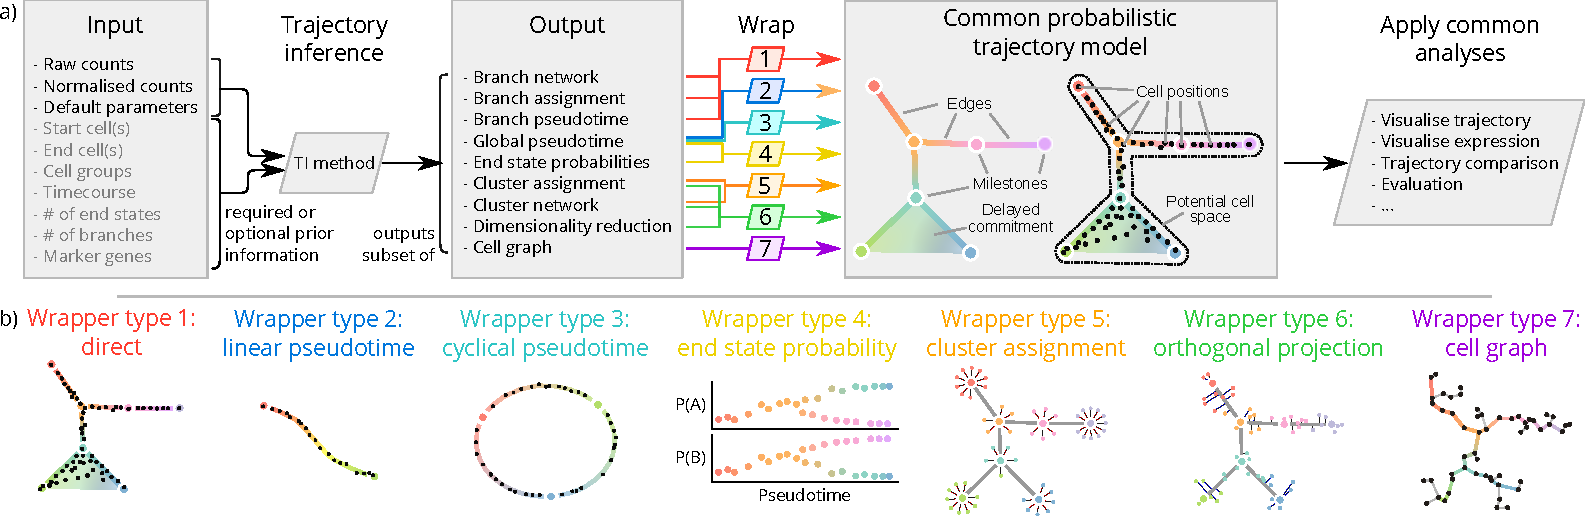
\includegraphics[width=\linewidth]{fig/supfigure_1.pdf}
	\caption{
		\textbf{A common interface for TI methods.}
		\textbf{a} The input and output of each TI method is standardized. As input, each TI method receives either raw or normalized counts, several parameters, and a selection of prior information. After its execution, a method uses one of the seven wrapper functions to transform its output to the common trajectory model. This common model then allows to perform common analysis functions on trajectory models produced by any TI method. \textbf{b} Illustrations of the specific transformations performed by each of the wrapper functions.
	}
	\label{fig:supfigure_1}
\end{figure}



\afterpage{%
	\clearpage% flush all other floats
	\ifodd\value{page}
%	\else% uncomment this else to get odd/even instead of even/odd
	\expandafter\afterpage% put it on the next page if this one is odd
	\fi
	{%
		\begin{figure}[tbh!]
			\centering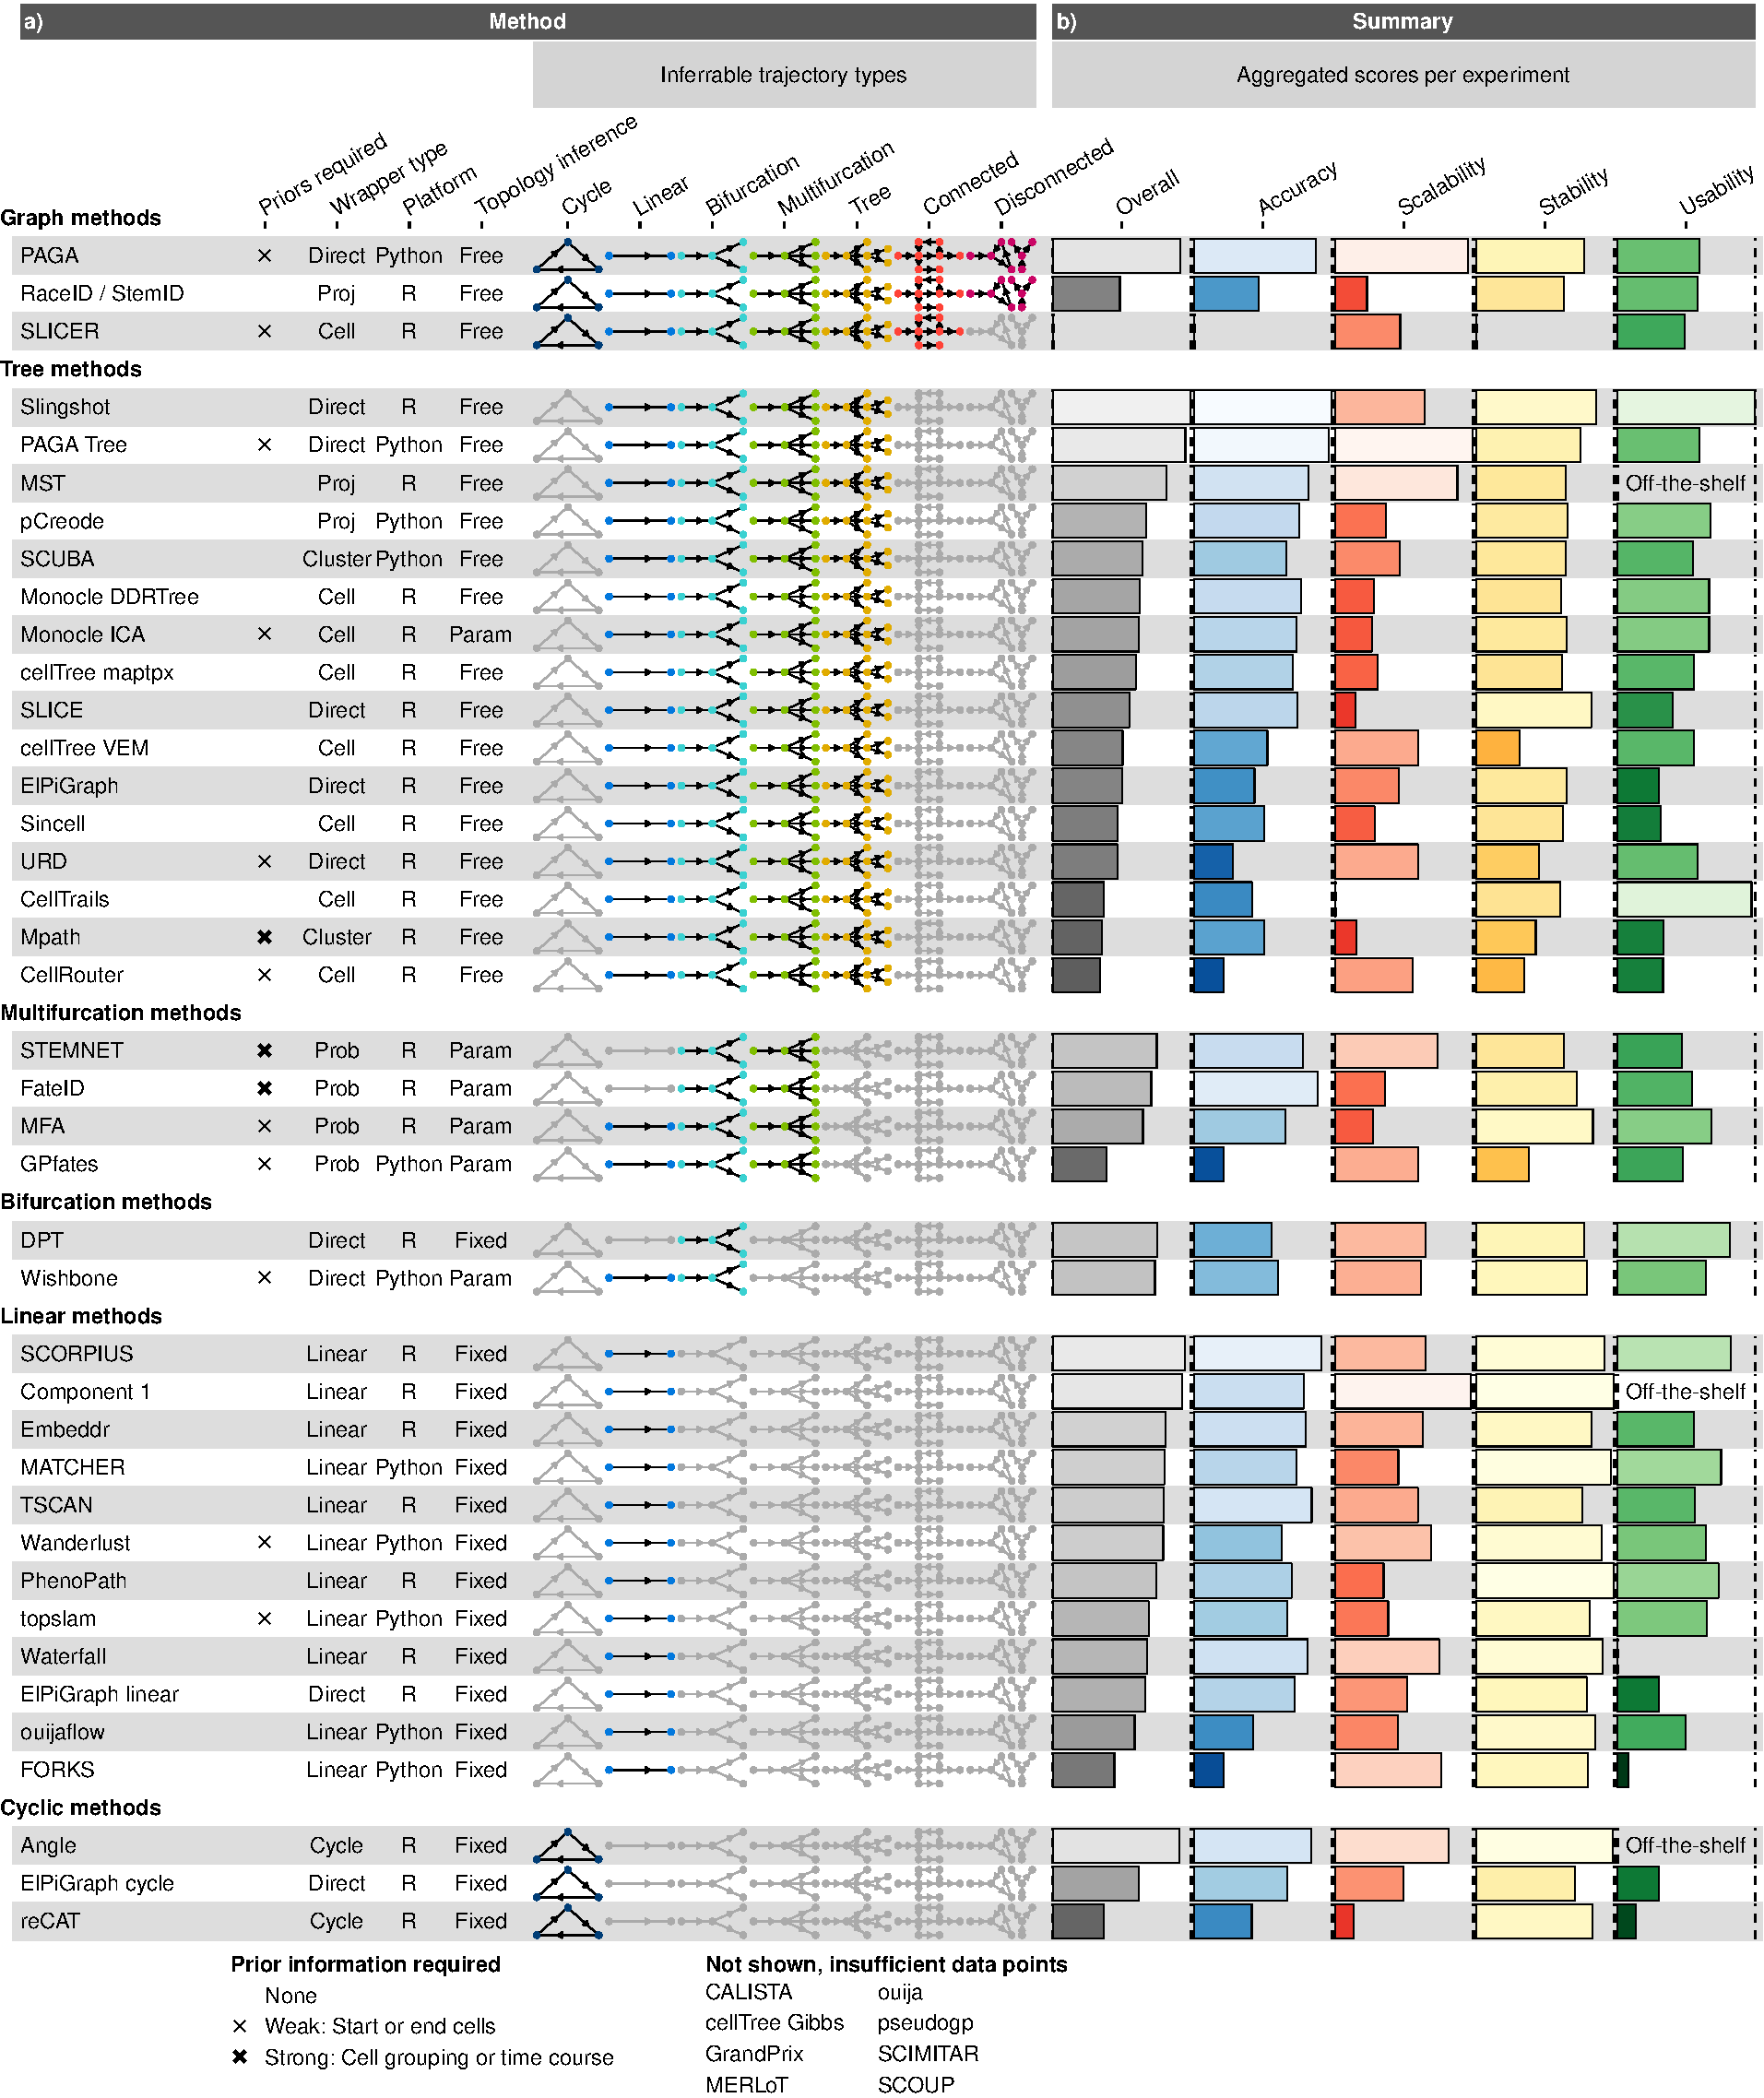
\includegraphics[height=.75\textheight]{fig/figure_2.pdf}
			\caption{
				\textbf{A characterization of the 45 methods evaluated in this study and their overall evaluation results.}
				\textbf{a}, We characterized the methods according to the wrapper type, their required priors, whether the inferred topology is constrained by the algorithm (fixed) or a parameter (param), and the types of inferable topologies. The methods are grouped vertically based on the most complex trajectory type they can infer. \textbf{b}, The overall results of the evaluation on four criteria: accuracy using a reference trajectory on real and synthetic data, scalability with increasing number of cells and features, stability across dataset subsamples and quality of the implementation. Methods that errored on more than 50$\%$ of the datasets are not included in this figure and are shown instead in Supplementary Figure~\hyperref[fig:suppfig_2]{3.1}.
			}
			\label{fig:figure_2}
		\end{figure}
		\clearpage
		\begin{figure}[tbh!]
			\centering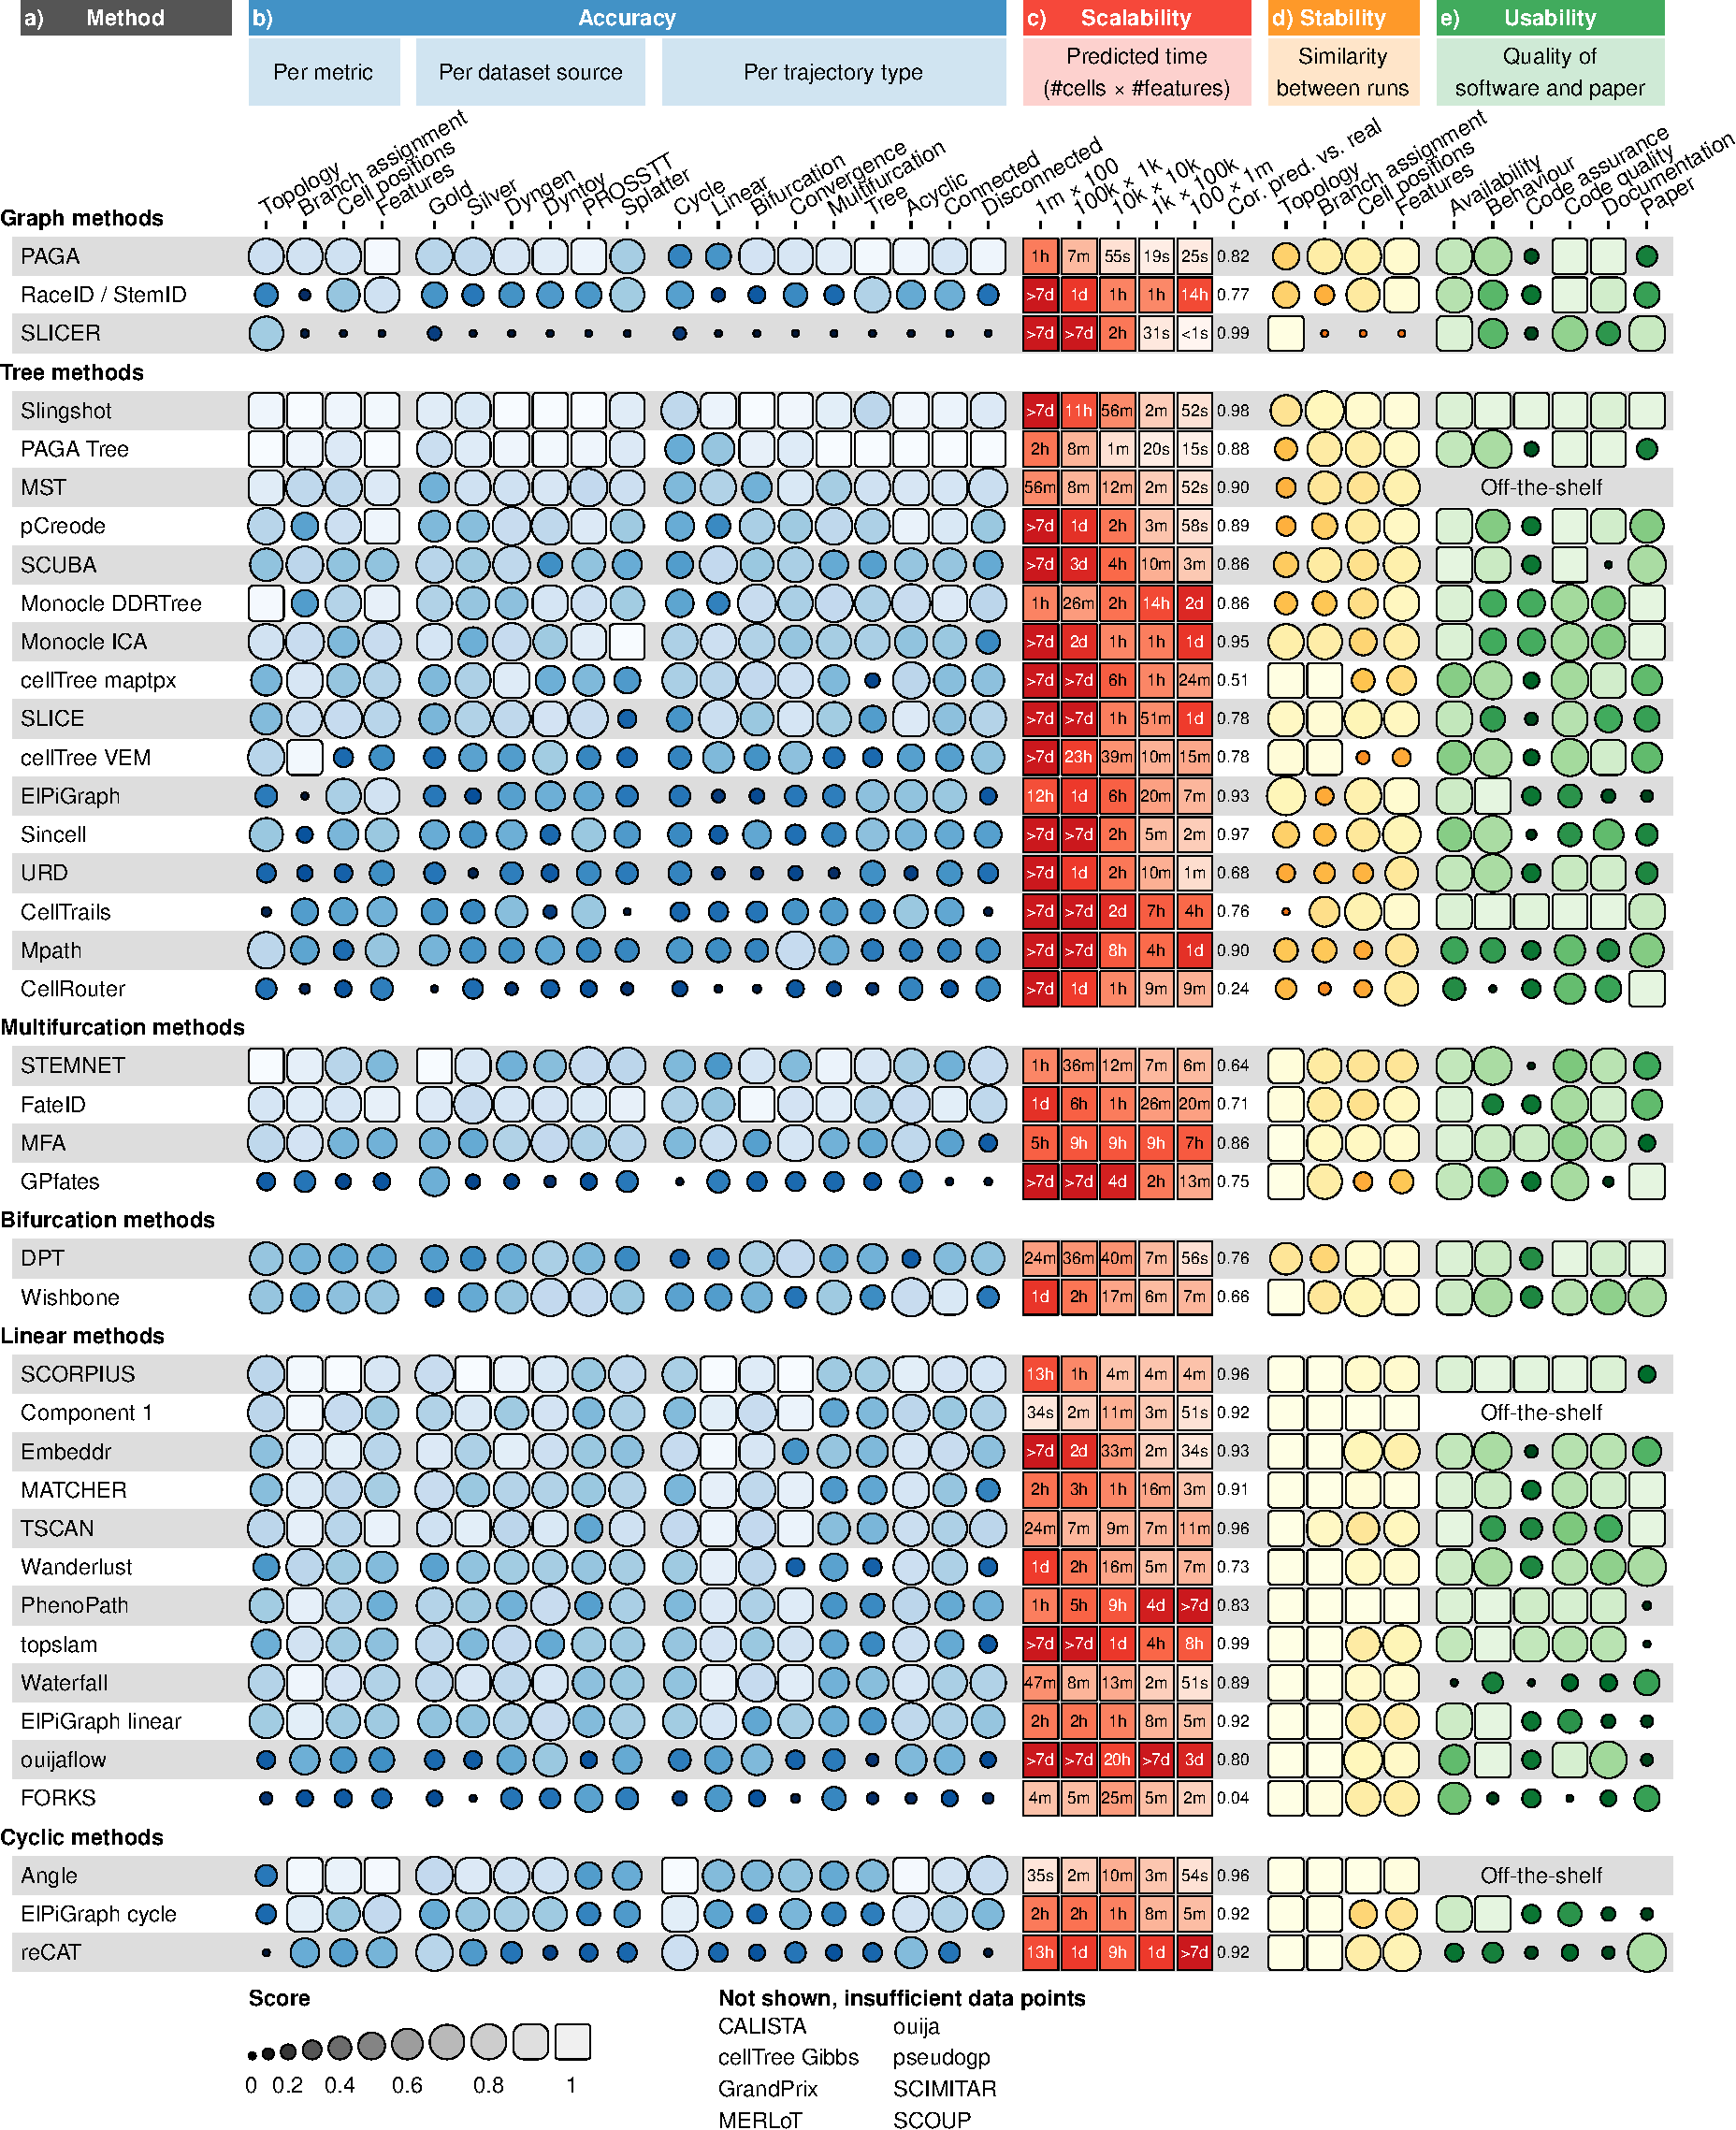
\includegraphics[height=.75\textheight]{fig/figure_3.pdf}
			\caption{	
				\textbf{Detailed results of the four main evaluation criteria: accuracy, scalability, stability and usability.}
				\textbf{a,} The names of the methods, ordered as in Figure \ref{fig:figure_2}. \textbf{b}, Accuracy of trajectory inference methods across metrics, dataset sources and dataset trajectory types. The performance of a method is generally more stable across dataset sources, but very variable depending on the metric and trajectory type. \textbf{c}, Predicted execution times for varying numbers of cells and features (no. of cells $\times$ no. of features). Predictions were made by training a regression model after running each method on bootstrapped datasets with varying numbers of cells and features. k, thousands; m, millions; cor, correlation. \textbf{d}, Stability results by calculating the average pairwise similarity between models inferred across multiple runs of the same method. \textbf{e}, Usability scores of the tool and corresponding manuscript, grouped per category. Off-the-shelf methods were directly implemented in R and thus do not have a usability score. 
			}
			\label{fig:figure_3}
		\end{figure}
		\clearpage
	}%
}



The largest difference between TI methods is whether a method fixes the topology and, if it does not, what kind of topology it can detect. We defined seven possible types of topology, ranging from very basic topologies (linear, cyclical and bifurcating) to the more complex ones (connected and disconnected graphs). Most methods either focus on inferring linear trajectories or limit the search to tree or less complex topologies, with only a selected few attempting to infer cyclic or disconnected topologies (Figure \ref{fig:figure_2}a).

We evaluated each method on four core aspects: (1) accuracy of a prediction, given a gold or silver standard on 110 real and 229 synthetic datasets; (2) scalability with respect to the number of cells and features (for example, genes); (3) stability of the predictions after subsampling the datasets; and (4) the usability of the tool in terms of software, documentation and the manuscript. Overall, we found a large diversity across the four evaluation criteria, with only a few methods, such as PAGA, Slingshot and SCORPIUS, performing well across the board (Figure \ref{fig:figure_2}b). We will discuss each evaluation criterion in more detail (Figure \ref{fig:figure_3} and Supplementary Figure~\hyperref[fig:suppfig_2]{3.1}), after which we conclude with guidelines for method users and future perspectives for method developers.


\subsection{Accuracy}

We defined several metrics to compare a prediction to a reference trajectory (Section~\ref{sec:dynb_supn1}). Based on an analysis of their robustness and conformity to a set of rules (Section~\ref{sec:dynb_supn1}), we chose four metrics each assessing a different aspect of a trajectory (Figure \ref{fig:figure_1}d): the topology (Hamming–Ipsen–Mikhailov, HIM), the quality of the assignment of cells to branches (F1branches), the cell positions (cordist) and the accuracy of the differentially expressed features along the trajectory (wcorfeatures). The data compendium consisted of both synthetic datasets, which offer the most exact reference trajectory, and real datasets, which provide the highest biological relevance. These real datasets come from a variety of single-cell technologies, organisms and dynamic processes, and contain several types of trajectory topologies (Supplementary Table~\hyperref[tab:supptable_2]{3.2}). Real datasets were classified as ‘gold standard’ if the reference trajectory was not extracted from the expression data itself, such as via cellular sorting or cell mixing \cite{tian_scrnaseqmixologybetter_2018}. All other real datasets were classified as ‘silver standard’. For synthetic datasets we used several data simulators, including a simulator of gene regulatory networks using a thermodynamic model of gene regulation \cite{schaffter_genenetweaversilicobenchmark_2011}. For each simulation, we used a real dataset as a reference, to match its dimensions, number of differentially expressed genes, drop-out rates and other statistical properties \cite{zappia_splattersimulationsinglecell_2017}.

We found that method performance was very variable across datasets, indicating that there is no ‘one-size-fits-all’ method that works well on every dataset (Figure \ref{fig:supfigure_3}a). Even methods that can detect most of the trajectory types, such as PAGA, RaceID/StemID and SLICER were not the best methods across all trajectory types (Figure \ref{fig:figure_3}b). The overall score between the different dataset sources was moderately to highly correlated (Spearman rank correlation between 0.5–0.9) with the scores on real datasets containing a gold standard (Figure \ref{fig:supfigure_3}b), confirming both the accuracy of the gold standard trajectories and the relevance of the synthetic data. On the other hand, the different metrics frequently disagreed with each other, with Monocle and PAGA Tree scoring better on the topology scores, whereas other methods, such as Slingshot, were better at ordering the cells and placing them into the correct branches (Figure \ref{fig:figure_3}b).


The performance of a method was strongly dependent on the type of trajectory present in the data (Figure \ref{fig:figure_3}b). Slingshot typically performed better on datasets containing more simple topologies, while PAGA, pCreode and RaceID/StemID had higher scores on datasets with trees or more complex trajectories (Figure \ref{fig:supfigure_3}c). This was reflected in the types of topologies detected by every method, as those predicted by Slingshot tended to contain less branches, whereas those detected by PAGA, pCreode and Monocle DDRTree gravitated towards more complex topologies (Figure \ref{fig:supfigure_3}d). This analysis therefore indicates that detecting the right topology is still a difficult task for most of these methods, because methods tend to be either too optimistic or too pessimistic regarding the complexity of the topology in the data.

The high variability between datasets, together with the diversity in detected topologies between methods, could indicate some complementarity between the different methods. To test this, we calculated the likelihood of obtaining a top model when using only a subset of all methods. A top model in this case was defined as a model with an overall score of at least 95$\%$ as the best model. On all datasets, using one method resulted in getting a top model about 27$\%$ of the time. This increased up to 74$\%$ with the addition of six other methods (Figure \ref{fig:figure_4}a). The result was a relatively diverse set of methods, containing both strictly linear or cyclic methods, and methods with a broad trajectory type range such as PAGA. We found similar indications of complementarity between the top methods on data containing only linear, bifurcation or multifurcating trajectories (Figure \ref{fig:figure_4}b), although in these cases less methods were necessary to obtain at least one top model for a given dataset. Altogether, this shows that there is considerable complementarity between the different methods and that users should try out a diverse set of methods on their data, especially when the topology is unclear a priori. Moreover, it also opens up the possibilities for new ensemble methods that utilize this complementarity.


\begin{figure}[tbh!]
	\centering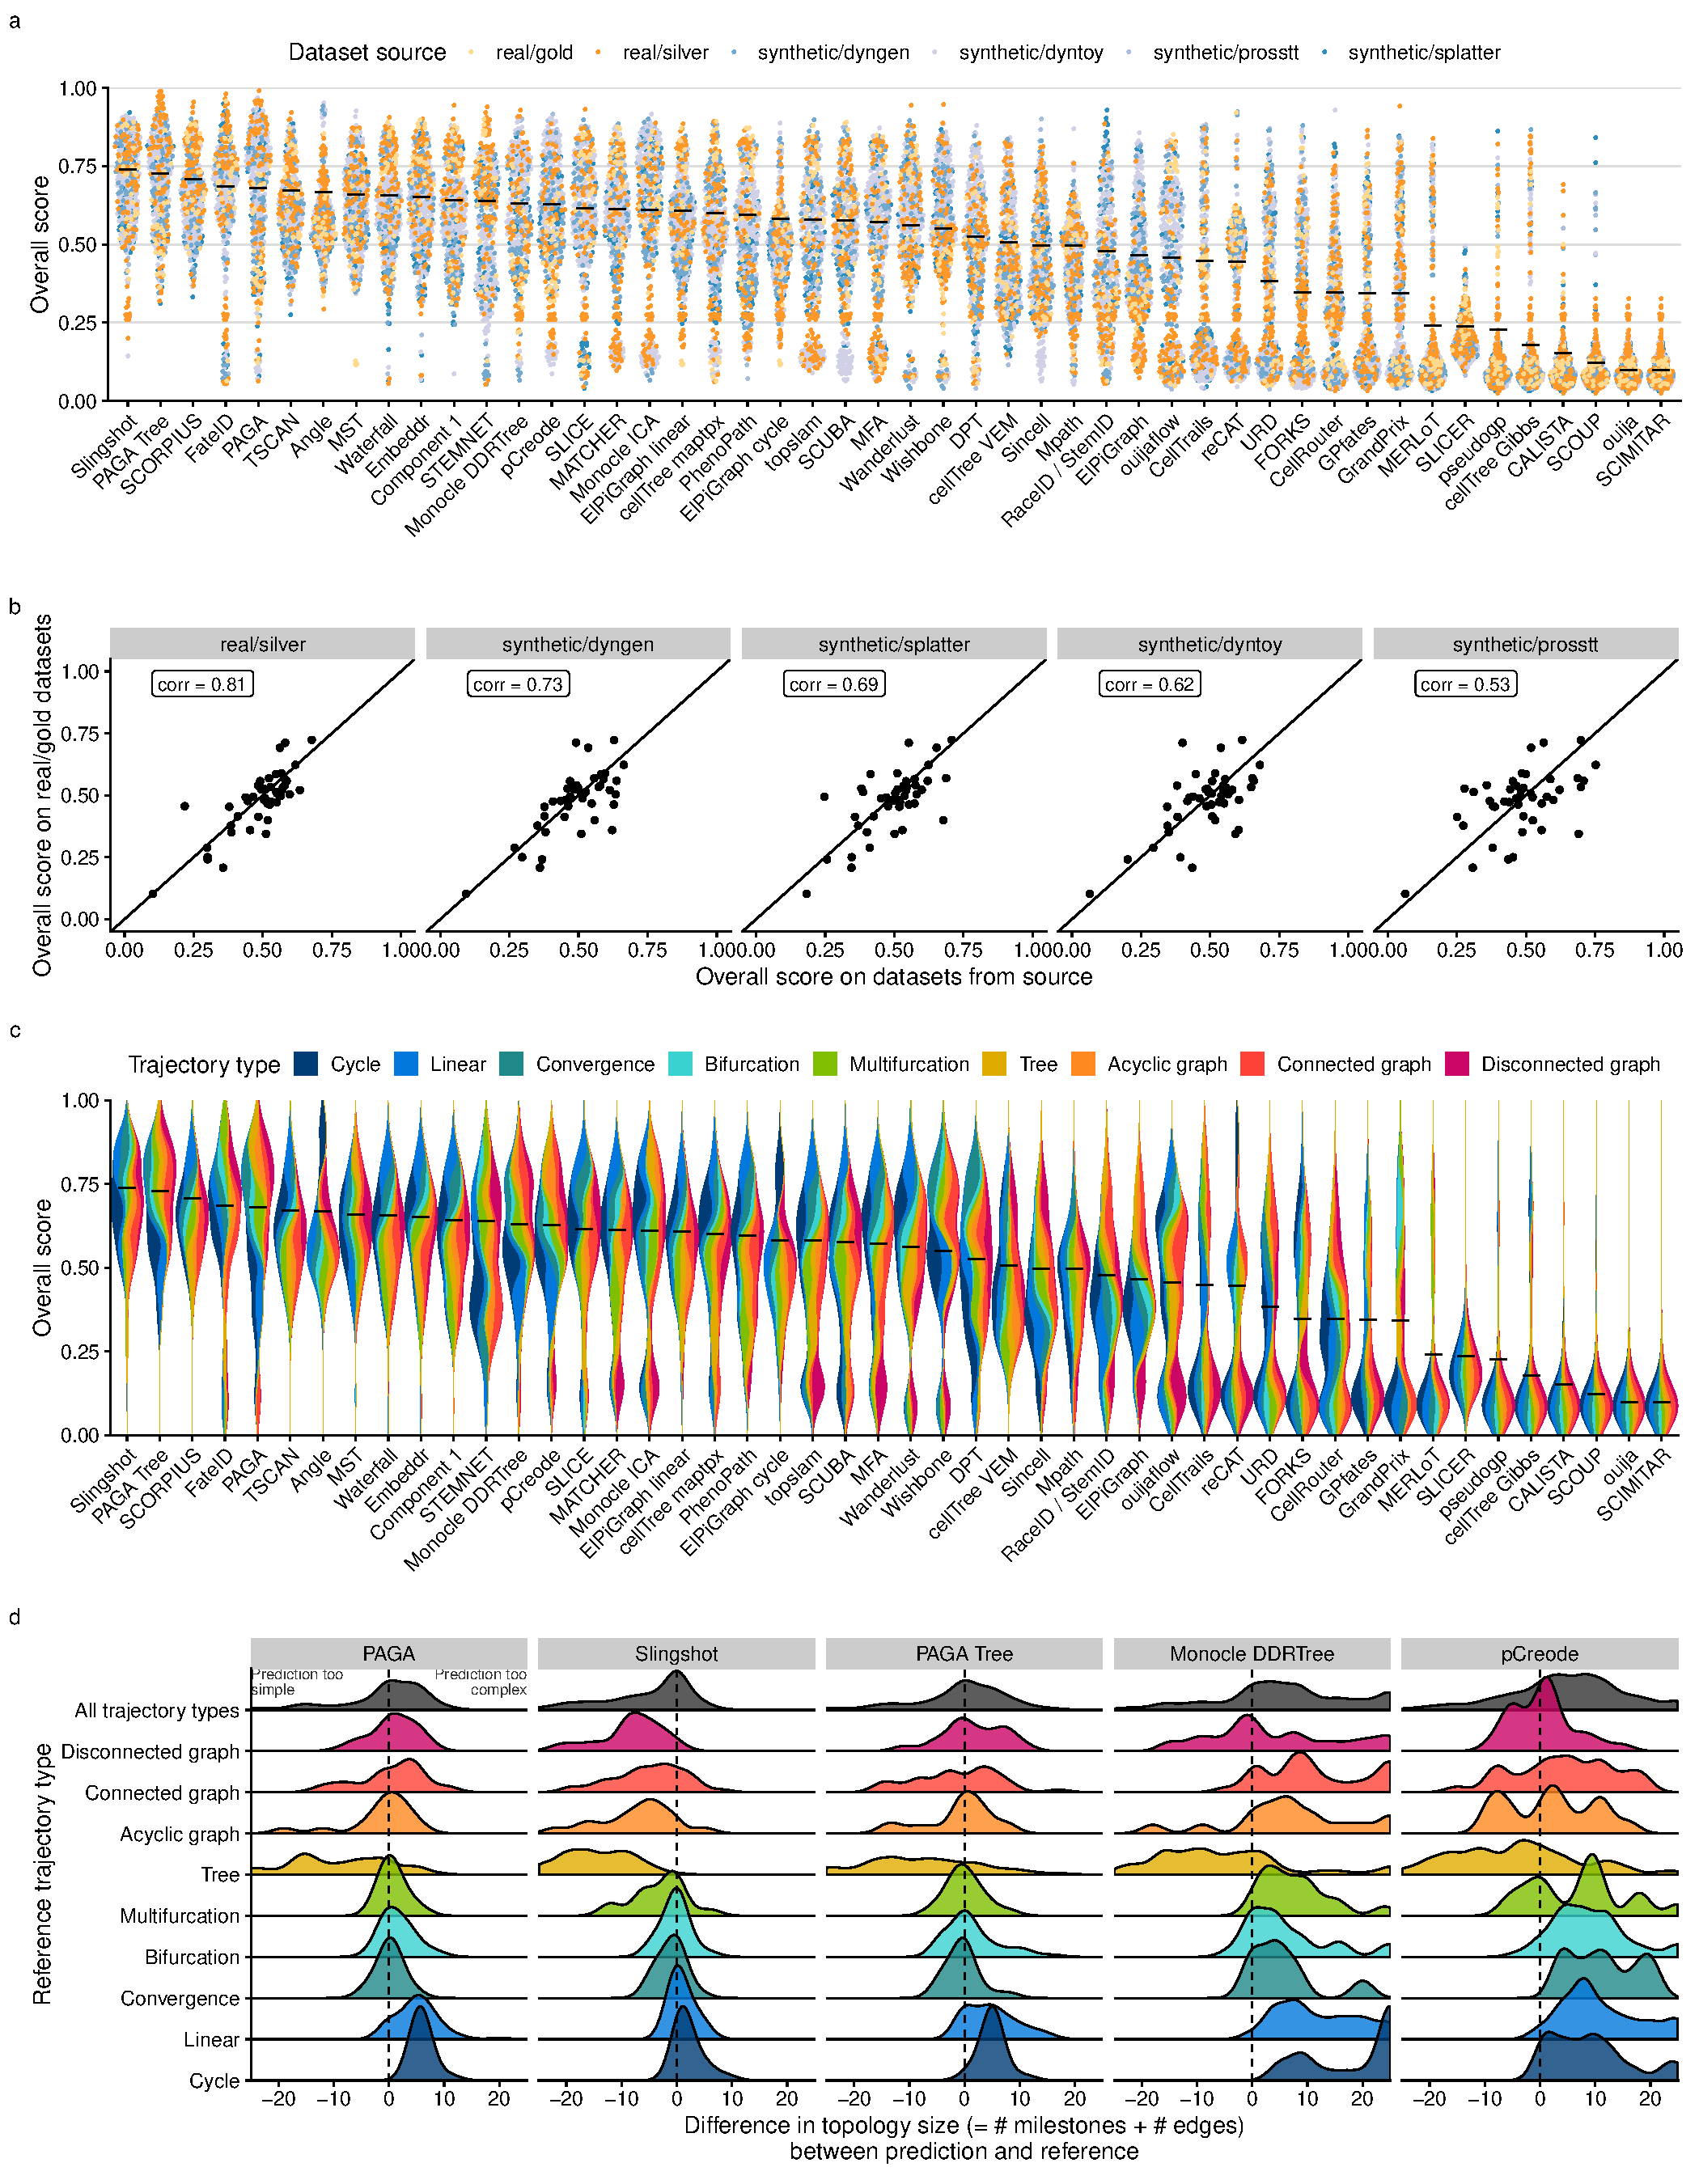
\includegraphics[width=\linewidth]{fig/supfigure_3.pdf}
	\caption{
		\textbf{Accuracy of trajectory inference methods.}
		\textbf{a} Overall score for all methods across 339 datasets, colored by the source of the datasets. Black line indicates the mean. \textbf{b} Similarity between the overall scores of all dataset sources, compared to real datasets with a gold standard, across all methods (n = 46, after filtering out methods that errored too frequently). Shown in the top left is the Pearson correlation. \textbf{c} Bias in the overall score towards trajectory types for all methods across 339 datasets. Black line indicates the mean. \textbf{d} Distributions of the difference in size between predicted and reference topologies. A positive difference means that the topology predicted by the method is more complex than the one in the reference.
	}
	\label{fig:supfigure_3}
\end{figure}

\begin{figure}[tbh!]
	\centering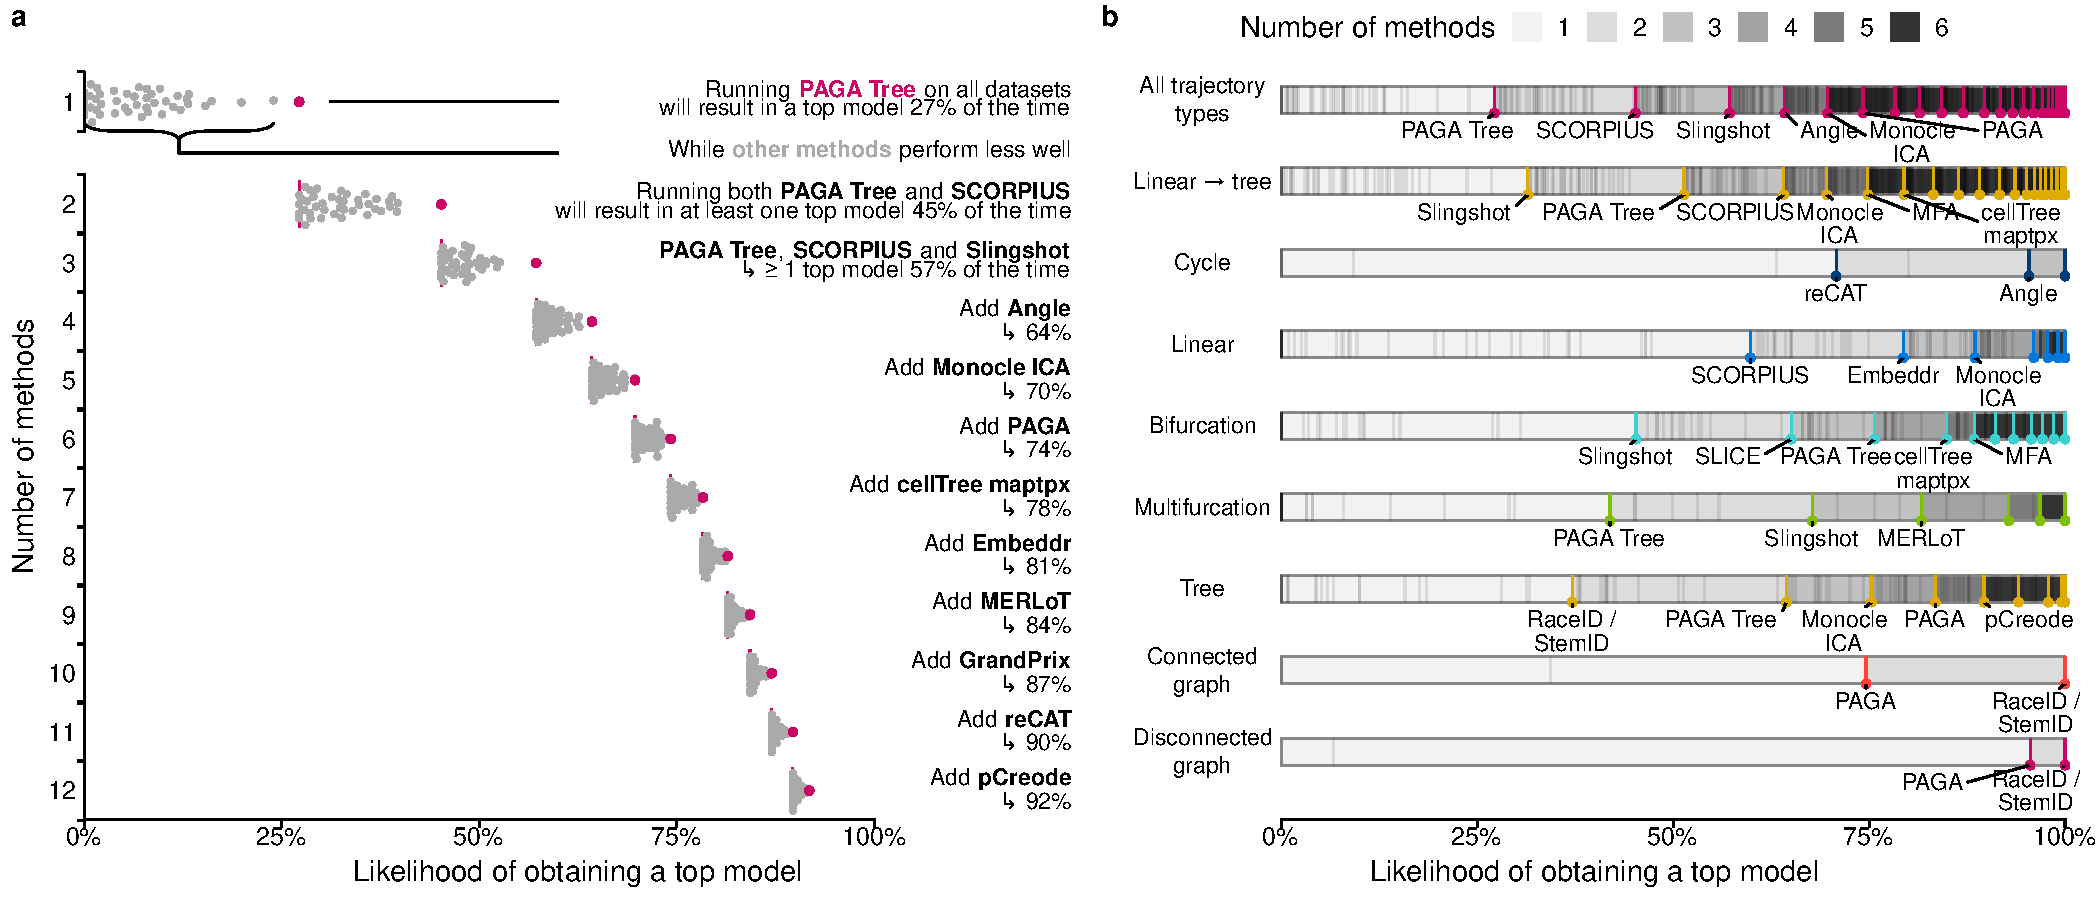
\includegraphics[width=\linewidth]{fig/figure_4.pdf}
	\caption{
		\textbf{Complementarity between different trajectory inference methods.}
		\textbf{a}, We assessed the likelihood for different combinations of methods to lead to a ‘top model’ (defined as a model with an overall score of at least 95$\%$ of the best model) when applied to all datasets. \textbf{b}, The likelihood for different combinations of methods to lead to a ‘top model’ was assessed separately on different trajectory types. For this figure, we did not include any methods requiring a cell grouping or a time course as prior information.
	}
	\label{fig:figure_4}
\end{figure}

\subsection{Scalability}

While early TI methods were developed at a time where profiling more than a thousand cells was exceptional, methods now have to cope with hundreds of thousands of cells, and perhaps soon with more than ten million \cite{svensson_exponentialscalingsinglecell_2018}. Moreover, the recent application of TI methods on multi-omics single-cell data also showcases the increasing demands on the number of features \cite{cao_jointprofilingchromatin_2018}. To assess the scalability, we ran each method on up- and downscaled versions of five distinct real datasets. We modeled the running time and memory usage using a Shape Constrained Additive Model \cite{pya_shapeconstrainedadditive_2015} (Figure \ref{fig:supfigure_4}a). As a control, we compared the predicted time (and memory) with the actual time (respectively memory) on all benchmarking datasets, and found that these were highly correlated overall (Spearman rank correlation >0.9, Figure \ref{fig:supfigure_5}, and moderately to highly correlated (Spearman rank correlation of 0.5–0.9) for almost every method, depending to what extent the execution of a method succeeded during the scalability experiments (Figure \ref{fig:figure_3}c and Supplementary Figure~\hyperref[fig:suppfig_2]{3.1}a).

\begin{figure}[tbh!]
	\centering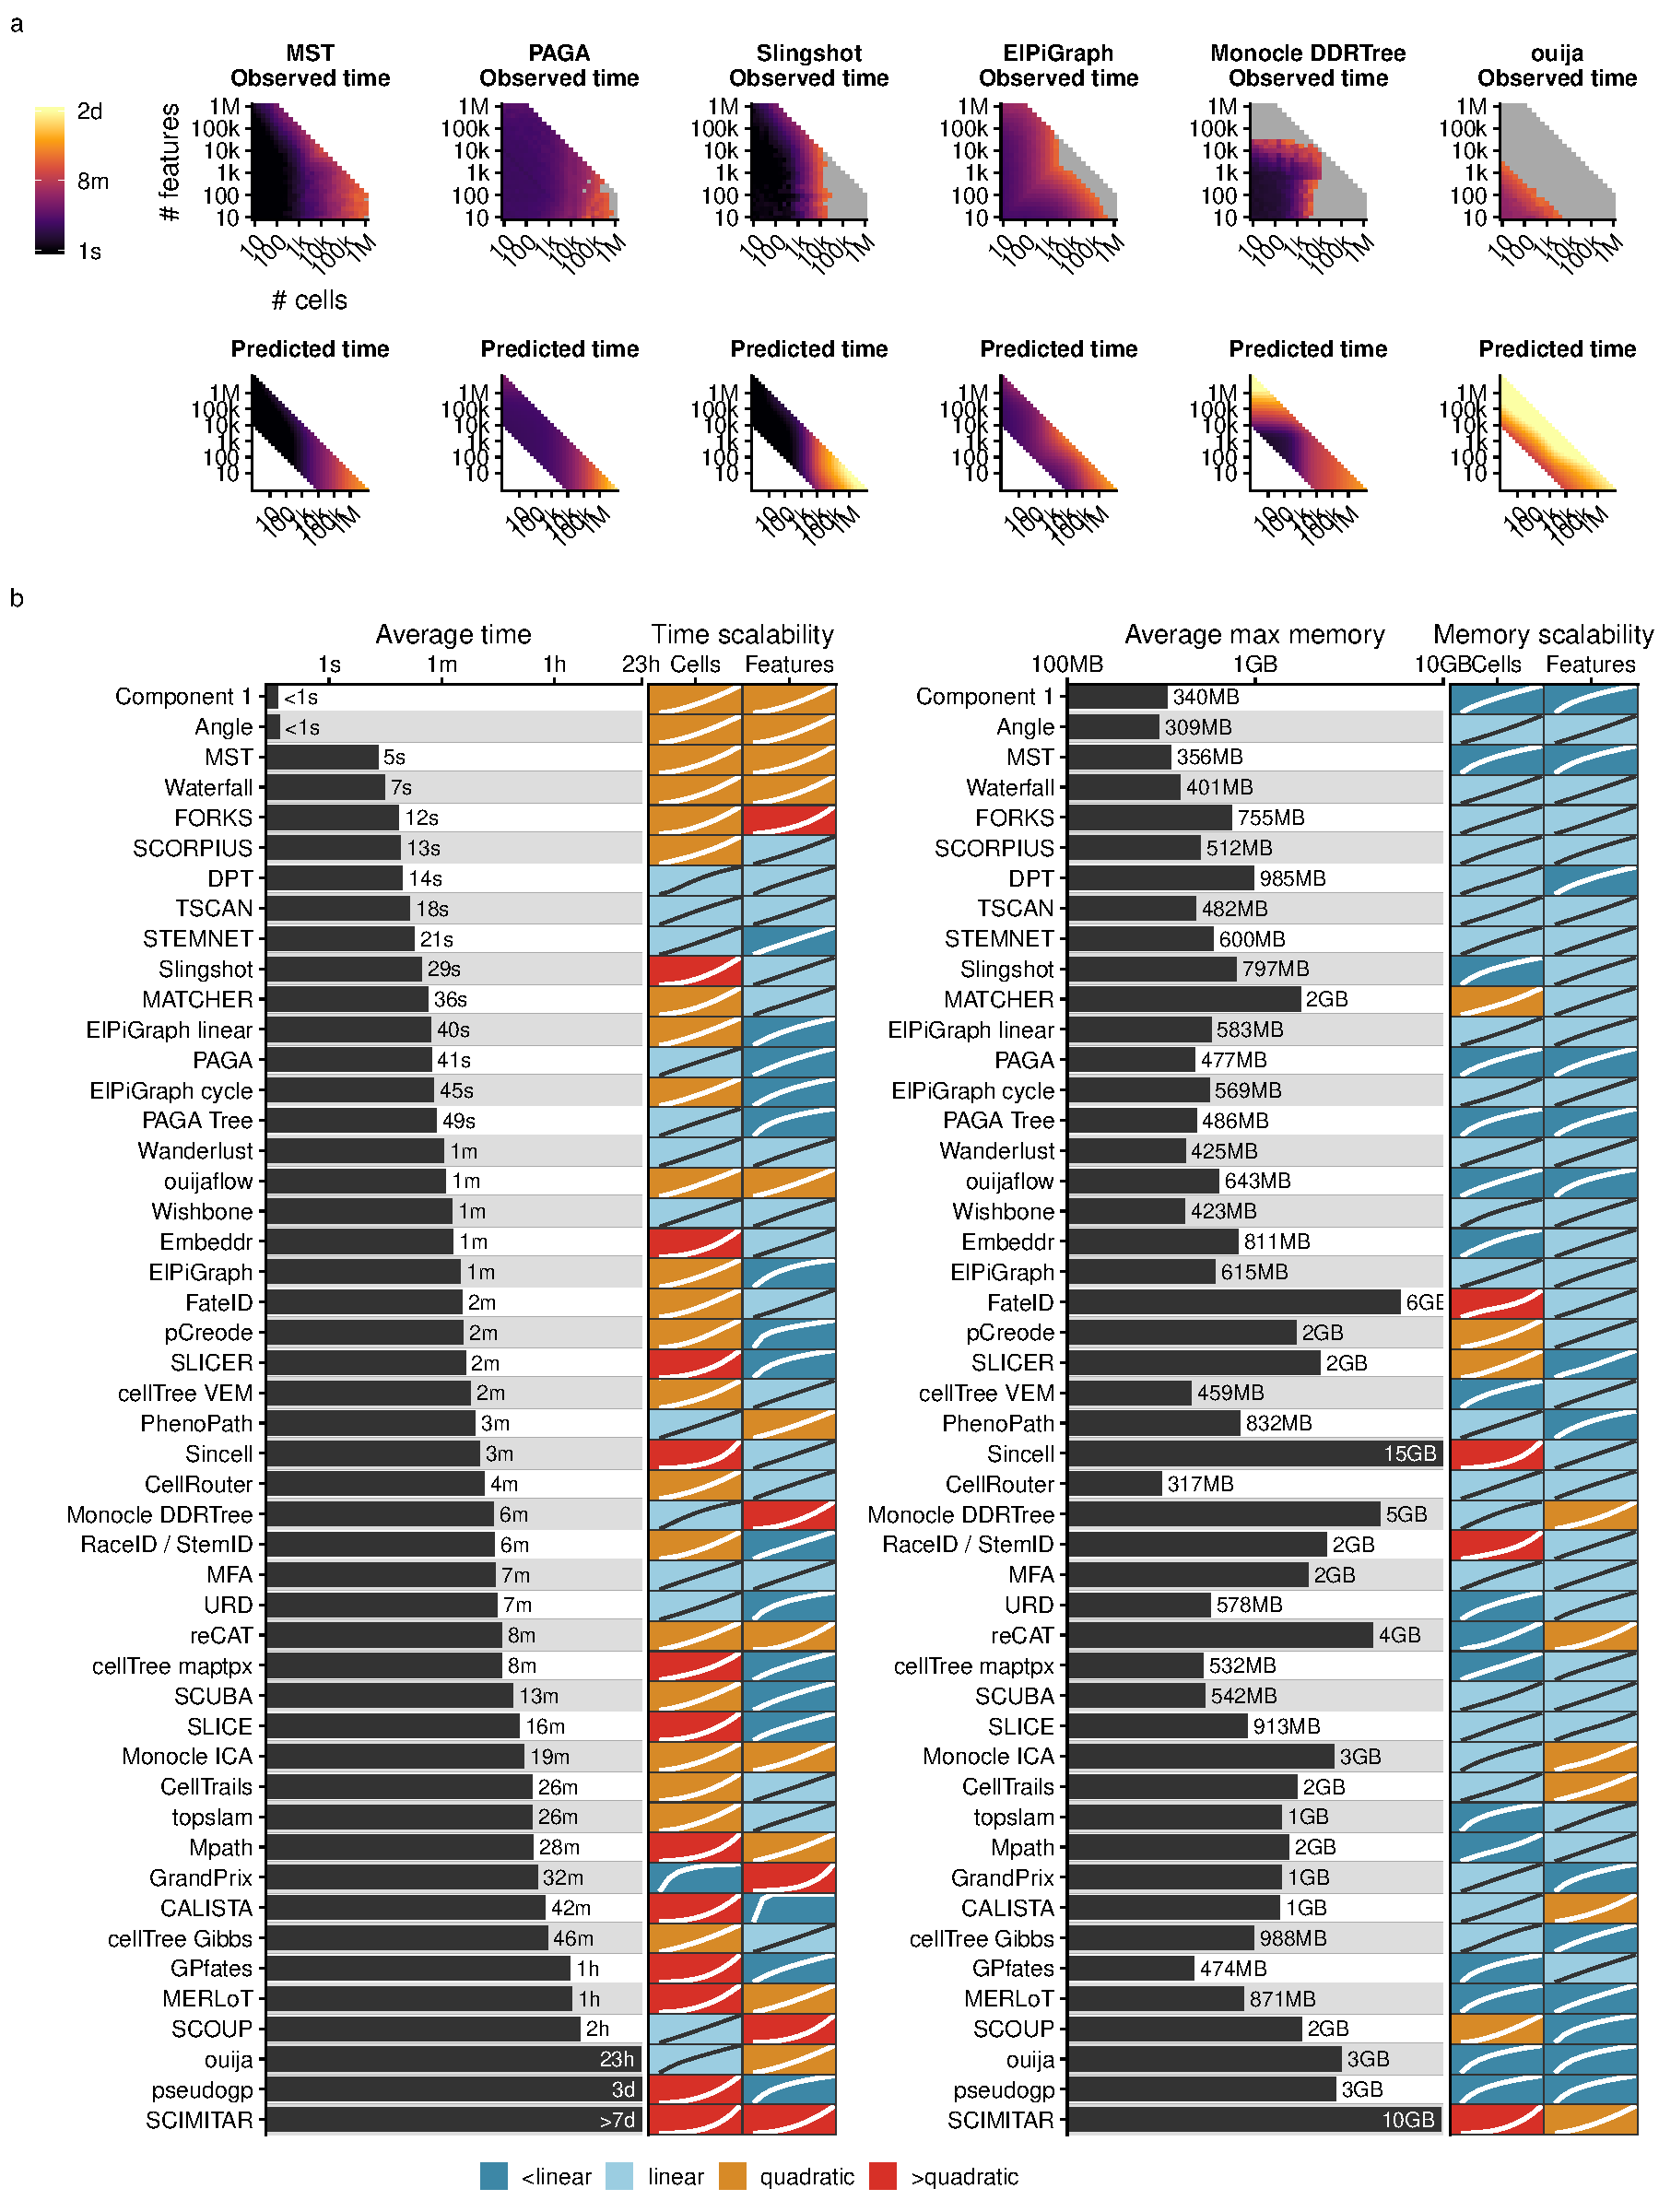
\includegraphics[width=0.9\linewidth]{fig/supfigure_4.pdf}
	\caption{
		\textbf{Scalability of trajectory inference methods.}
		\textbf{a} Three examples of average observed running times across five datasets (left) and the predicted running time (right). \textbf{b} Overview of the scalability results of all methods, ordered by their average predicted running time from (a). We predicted execution times and memory usage for each method with increasing number of features or cells, and used these values to classify each method into sublinear, linear, quadratic and superquadratic based on the shape of the curve.
	}
	\label{fig:supfigure_4}
\end{figure}


\begin{figure}[tbh!]
	\centering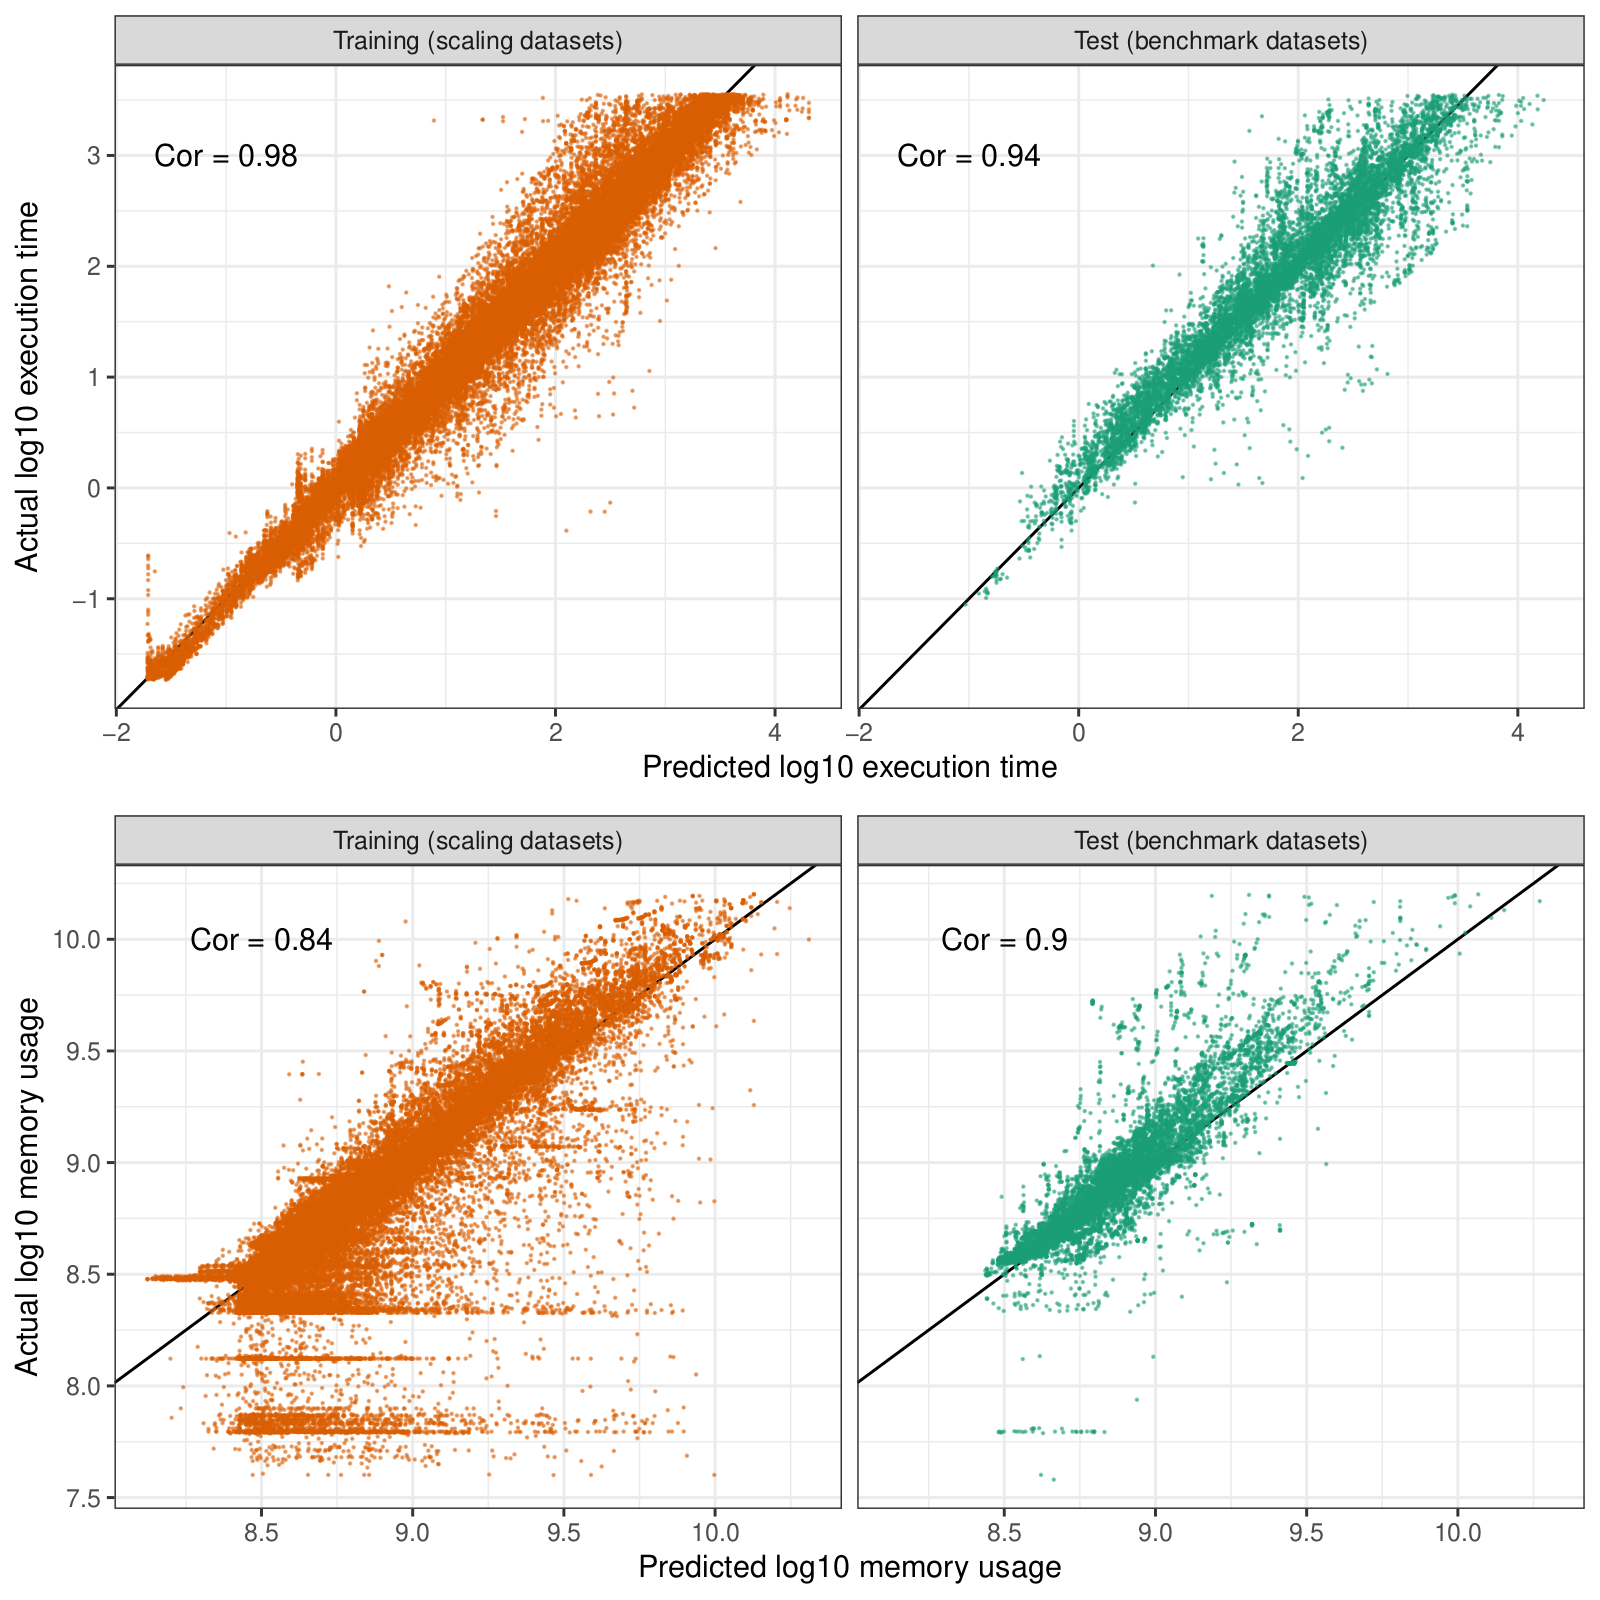
\includegraphics[width=0.6\linewidth]{fig/supfigure_5.png}
	\caption{
		\textbf{Agreement between actual values and predictions for execution times and memory usage.}
		We created a predictive model of the running time and memory usage based on a set of scaling datasets (left), and validated this model based on the similarity of the predictions and actual values on all benchmark datasets (right). Shown are the values for each method and dataset (n = 65618 for training, n = 11939 for test). Top left indicates the Pearson correlation coefficient.
	}
	\label{fig:supfigure_5}
\end{figure}

We found that the scalability of most methods was overall very poor, with most graph and tree methods not finishing within an hour on a dataset with ten thousand cells and ten thousand features (Figure \ref{fig:figure_3}c), which is around the size of a typical droplet-based single-cell dataset \cite{svensson_exponentialscalingsinglecell_2018}. Running times increased further with increasing number of cells, with only a handful of graph/tree methods completing within a day on a million cells (PAGA, PAGA Tree, Monocle DDRTree, Stemnet and GrandPrix). Some methods, such as Monocle DDRTree and GrandPrix, also suffered from unsatisfactory running times when given a high number of features.

Methods with a low running time typically had two defining aspects: they had a linear time complexity with respect to the features and/or cells, and adding new cells or features led to a relatively low increase in time (Figure \ref{fig:supfigure_4}b). We found that more than half of all methods had a quadratic or superquadratic complexity with respect to the number of cells, which would make it difficult to apply any of these methods in a reasonable time frame on datasets with more than a thousand cells (Figure \ref{fig:supfigure_4}b).

We also assessed the memory requirements of each method (Supplementary Figure~\hyperref[fig:suppfig_2]{3.1}c). Most methods had reasonable memory requirements for modern workstations or computer clusters ($\leq$12 GB) with PAGA and STEMNET in particular having a low memory usage with both a high number of cells or a high number of features. Notably, the memory requirements were very high for several methods on datasets with high numbers of cells (RaceID/StemID, pCreode and MATCHER) or features (Monocle DDRTree, SLICE and MFA).

Altogether, the scalability analysis indicated that the dimensions of the data are an important factor in the choice of method, and that method development should pay more attention to maintaining reasonable running times and memory usage.

\subsection{Stability}

It is not only important that a method is able to infer an accurate model in a reasonable time frame, but also that it produces a similar model when given very similar input data. To test the stability of each method, we executed each method on ten different subsamples of the datasets (95$\%$ of the cells, 95$\%$ of the features), and calculated the average similarity between each pair of models using the same scores used to assess the accuracy of a trajectory (Figure \ref{fig:figure_3}d).

Given that the trajectories of methods that fix the topology either algorithmically or through a parameter are already very constrained, it is to be expected that such methods tend to generate very stable results. Nonetheless, some fixed topology methods still produced slightly more stable results, such as SCORPIUS and MATCHER for linear methods and MFA for multifurcating methods. Stability was much more diverse among methods with a free topology. Slingshot produced more stable models than PAGA (Tree), which in turn produced more stable results than pCreode and Monocle DDRTree.

\subsection{Usability}

While not directly related to the accuracy of the inferred trajectory, it is also important to assess the quality of the implementation and how user-friendly it is for a biological user \cite{taschuk_tensimplerules_2017}. We scored each method using a transparent checklist of important scientific and software development practices, including software packaging, documentation, automated code testing and publication into a peer-reviewed journal (Table \ref{tab:scoresheet}). It is important to note that there is a selection bias in the tools chosen for this analysis, as we did not include a substantial set of tools due to issues with installation, code availability and executability on a freely available platform (which excludes MATLAB). The reasons for not including certain tools are all discussed on our repository (\url{https://github.com/dynverse/dynmethods/issues?q=label:unwrappable}). Installation issues seem to be quite general in bioinformatics \cite{mangul_comprehensiveanalysisusability_2018} and the trajectory inference field is no exception.

We found that most methods fulfilled the basic criteria, such as the availability of a tutorial and elemental code quality criteria (Figure \ref{fig:figure_3}d and Figure~\ref{fig:supfigure_6}). While recent methods had a slightly better quality score than older methods, several quality aspects were consistently lacking for the majority of the methods (Figure~\ref{fig:supfigure_6} right) and we believe that these should receive extra attention from developers. Although these outstanding issues covered all five categories, code assurance and documentation in particular were problematic areas, notwithstanding several studies pinpointing these as good practices \cite{wilson_bestpracticesscientific_2014,artaza_top10metrics_2016}. Only two methods had a nearly perfect usability score (Slingshot and Celltrails), and these could be used as an inspiration for future methods. We observed no clear relation between usability and method accuracy or usability (Figure \ref{fig:figure_2}b).


\begin{figure}[tbh!]
	\centering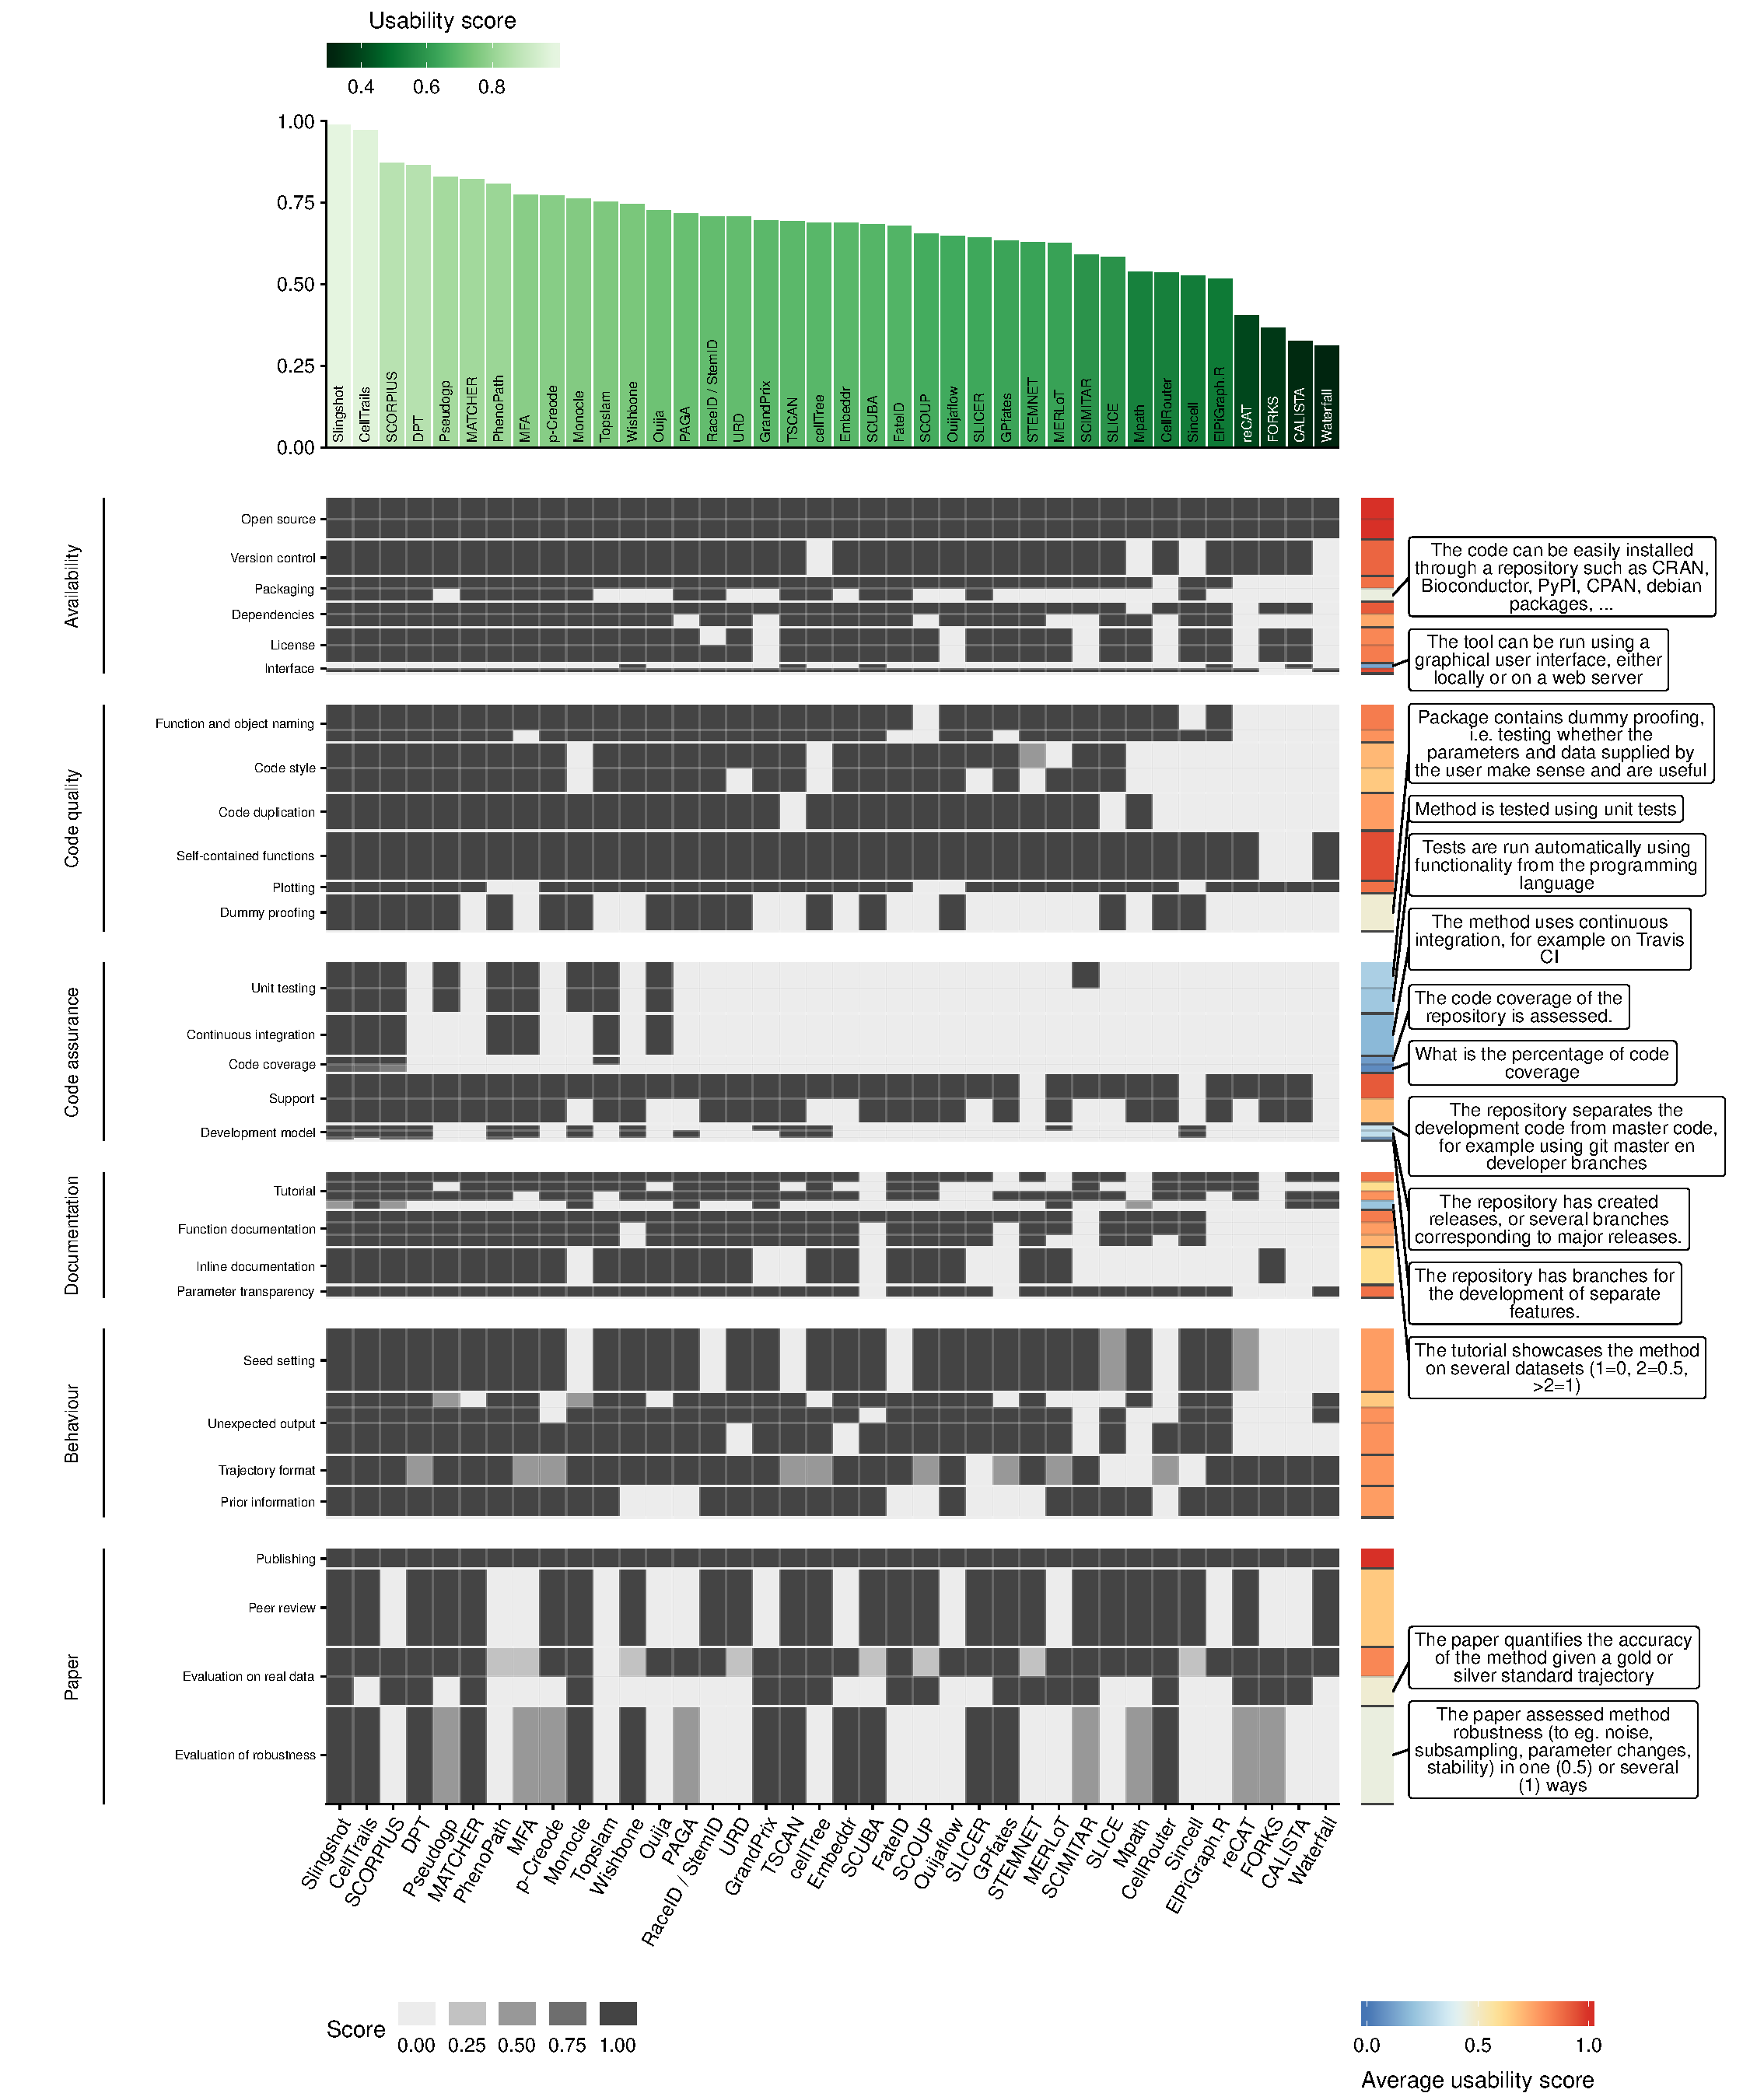
\includegraphics[width=0.9\linewidth]{fig/supfigure_6.pdf}
	\caption{
		\textbf{Usability of trajectory inference methods.}
		Shown is the score given for each method on every item from the usability score sheet(Table~\ref{tab:scoresheet}). Each aspect of the quality control was part of a category, and each category was weighted so that it contributed equally to the final quality score. Within each  category,  each  aspect  also  received  a  weight  depending  on  how  often  it  was mentioned  in  a set  of  papers  discussing  good practices in tool development and evaluation. This is represented in the plot as the height on the y-axis. Top: Average usability score for each method. Right: The average score of each quality control item. Shown into more detail are those items which had an average score lower than 0.5.
	}
	\label{fig:supfigure_6}
\end{figure}

\begin{table}[tbh!]
	\caption{\textbf{Scoring sheet for assessing usability of trajectory inference methods.} Each quality aspect was given a weight based on how many times it was mentioned in a set of articles discussing best practices for tool development. Part 1.} \label{tab:scoresheet}
	
	\centering\begingroup\fontsize{7}{9}\selectfont
	
	\begin{tabular}{p{2.5cm}p{8cm}p{1.5cm}}
		\toprule
		Aspect & Items & References \\ \midrule
		
		\multicolumn{3}{l}{\textbf{Availability}}\\*
		
		Open source & (1) Method's code is freely available (2) The code can be run on a freely available platform & \cite{lee_rpackagespackagedevelopment_2017,wilson_bestpracticesscientific_2014,taschuk_tensimplerules_2017,wickham_packagesorganizetest_2015,artaza_top10metrics_2016,silva_generalguidelinesbiomedical_2017,jimenez_foursimplerecommendations_2017}\\*
		
		Version control & The code is available on a public version controlled repository, such as Github & \cite{lee_rpackagespackagedevelopment_2017,wilson_bestpracticesscientific_2014,taschuk_tensimplerules_2017,wickham_packagesorganizetest_2015,artaza_top10metrics_2016,silva_generalguidelinesbiomedical_2017}\\*
		
		Packaging & (1) The code is provided as a "package", exposing functionality through functions or shell commands (2) The code can be easily installed through a repository such as CRAN, Bioconductor, PyPI, CPAN, debian packages, … & \cite{lee_rpackagespackagedevelopment_2017,wickham_packagesorganizetest_2015,jimenez_foursimplerecommendations_2017,silva_generalguidelinesbiomedical_2017}\\*
		
		Dependencies & (1) Dependencies are clearly stated in the tutorial or in the code (2) Dependencies are automatically installed & \cite{taschuk_tensimplerules_2017,wickham_packagesorganizetest_2015,artaza_top10metrics_2016,karimzadeh_topconsiderationscreating_2018}\\*
		
		License & (1) The code is licensed (2) License allows academic use & \cite{lee_rpackagespackagedevelopment_2017,taschuk_tensimplerules_2017,wickham_packagesorganizetest_2015,artaza_top10metrics_2016,silva_generalguidelinesbiomedical_2017,jimenez_foursimplerecommendations_2017}\\*
		
		Interface & (1) The tool can be run using a graphical user interface, either locally or on a web server (2) The tool can be run through the command line or through a programming language & \cite{silva_generalguidelinesbiomedical_2017}\\
		
		\midrule
		\multicolumn{3}{l}{\textbf{Code quality}} \\*
		
		Function and object naming & (1) Functions/commands have well chosen names (2) Arguments/parameters have well chosen names & \cite{wilson_bestpracticesscientific_2014,wickham_packagesorganizetest_2015}\\*
		
		Code style & (1) Code has a consistent style (2) Code follows (basic) good practices in the programming language of choice, for example PEP8 or the tidyverse style guide & \cite{wilson_bestpracticesscientific_2014,wickham_packagesorganizetest_2015,artaza_top10metrics_2016}\\*
		
		Code duplication & Duplicated code is minimal & \cite{wilson_bestpracticesscientific_2014,wickham_packagesorganizetest_2015}\\
		
		Self-contained functions & The method is exposed to the user as self-contained functions or commands & \cite{anderson_writinggreatscientific_2016,taschuk_tensimplerules_2017,silva_generalguidelinesbiomedical_2017}\\*
		
		Plotting & Plotting functions are provided for the final and/or intermediate results & \\*
		
		Dummy proofing & Package contains dummy proofing, i.e. testing whether the parameters and data supplied by the user make sense and are useful & \cite{lee_rpackagespackagedevelopment_2017,karimzadeh_topconsiderationscreating_2018}\\
		
		\midrule
		\multicolumn{3}{l}{\textbf{Code assurance}} \\*
		
		Unit testing & Method is tested using unit tests & \cite{lee_rpackagespackagedevelopment_2017,wilson_bestpracticesscientific_2014,anderson_writinggreatscientific_2016,wickham_packagesorganizetest_2015,silva_generalguidelinesbiomedical_2017}\\*
		
		Unit testing & Tests are run automatically using functionality from the programming language & \cite{lee_rpackagespackagedevelopment_2017,wilson_bestpracticesscientific_2014,anderson_writinggreatscientific_2016,wickham_packagesorganizetest_2015,silva_generalguidelinesbiomedical_2017}\\*
		
		Continuous integration & The method uses continuous integration, for example on Travis CI & \cite{beaulieu-jones_reproducibilitycomputationalworkflows_2017,wickham_packagesorganizetest_2015,artaza_top10metrics_2016,silva_generalguidelinesbiomedical_2017}\\*
		
		Code coverage & (1) The code coverage of the repository is assessed. (2) What is the percentage of code coverage & \\
		
		\bottomrule
	\end{tabular}
	\endgroup{}
\end{table}


\begin{table}[tbh!]
	\caption{\textbf{Scoring sheet for assessing usability of trajectory inference methods.} Part 2.} \label{tab:scoresheet2}
	
	\centering\begingroup\fontsize{7}{9}\selectfont
	
	\begin{tabular}{p{2.5cm}p{8cm}p{1.5cm}}
		\toprule
		Aspect & Items & References \\ \midrule
		
		\multicolumn{3}{l}{\textbf{Documentation}} \\*
		
		Support & (1) There is a support ticket system, for example on Github (2) The authors respond to tickets and issues are resolved within a reasonable time frame & \cite{wilson_bestpracticesscientific_2014,wickham_packagesorganizetest_2015,artaza_top10metrics_2016,silva_generalguidelinesbiomedical_2017,jimenez_foursimplerecommendations_2017}\\*
		
		Development model & (1) The repository separates the development code from master code, for example using git master en developer branches (2) The repository has created releases, or several branches corresponding to major releases. (3) The repository has branches for the development of separate features. & \cite{driessen_successfulgitbranching_2010}\\*
		
		Tutorial & (1) A tutorial or vignette is available (2) The tutorial has example results (3) The tutorial has real example data (4) The tutorial showcases the method on several datasets (1=0, 2=0.5, >2=1) & \cite{wickham_packagesorganizetest_2015,silva_generalguidelinesbiomedical_2017,jimenez_foursimplerecommendations_2017,karimzadeh_topconsiderationscreating_2018,boulesteix_tensimplerules_2015}\\*
		
		Function documentation & (1) The purpose and usage of functions/commands is documented (2) The parameters of functions/commands are documented (3) The output of functions/commands is documented & \cite{wilson_bestpracticesscientific_2014,taschuk_tensimplerules_2017,wickham_packagesorganizetest_2015,silva_generalguidelinesbiomedical_2017,karimzadeh_topconsiderationscreating_2018}\\*
		
		Inline documentation & Inline documentation is present in the code & \cite{wilson_bestpracticesscientific_2014,taschuk_tensimplerules_2017,wickham_packagesorganizetest_2015,silva_generalguidelinesbiomedical_2017,karimzadeh_topconsiderationscreating_2018}\\*
		
		Parameter transparency & All important parameters are exposed to the user & \cite{taschuk_tensimplerules_2017}\\
		
		\midrule
		\multicolumn{3}{l}{\textbf{Behaviour}} \\*
		
		Seed setting & The method does not artificially become deterministic (1), for example by setting some (0.5) or a lot (0) of seeds & \cite{puget_greendiceare_2016}\\*
		
		Unexpected output & (1) No unexpected output messages are generated by the method (2) No unexpected files, folders or plots are generated (3) No unexpected warnings during runtime or compilation are generated & \cite{artaza_top10metrics_2016}\\*
		
		Trajectory format & The postprocessing necessary to extract the relevant output from the method is minimal (1), moderate (0.5) or extensive (0) & \\*
		
		Prior information & Prior information is required (0), optional (1) or not required (1) & \\*
		
		\midrule
		\multicolumn{3}{l}{\textbf{Paper}} \\*
		
		Publishing & The method is published & \\*
		
		Peer review & The paper is published in a peer-reviewed journal & \cite{karimzadeh_topconsiderationscreating_2018,gannon_essentialrolepeer_2001,baldwin_refereeswetrust_2017}\\*
		
		Evaluation on real data & (1) The paper shows the method's usefulness on several (1), one (0.25) or no real datasets. (2) The paper quantifies the accuracy of the method given a gold or silver standard trajectory & \cite{aniba_issuesbioinformaticsbenchmarking_2010,jelizarow_overoptimismbioinformaticsillustration_2010}\\*
		
		Evaluation of robustness & The paper assessed method robustness (to eg. noise, subsampling, parameter changes, stability) in one (0.5) or several (1) ways & \cite{karimzadeh_topconsiderationscreating_2018,aniba_issuesbioinformaticsbenchmarking_2010,boulesteix_tensimplerules_2015,jelizarow_overoptimismbioinformaticsillustration_2010}\\
		
		\bottomrule
	\end{tabular}
	\endgroup{}
\end{table}


\section{Discussion}

In this study, we presented a large-scale evaluation of the performance of 45 TI methods. By using a common trajectory representation and four metrics to compare the methods’ outputs, we were able to assess the accuracy of the methods on more than 200 datasets. We also assessed several other important quality measures, such as the quality of the method’s implementation, the scalability to hundreds of thousands of cells and the stability of the output on small variations of the datasets.

Based on the results of our benchmark, we propose a set of practical guidelines for method users (Figure \ref{fig:figure_5} and \url{https://guidelines.dynverse.org}). We postulate that, as a method’s performance is heavily dependent on the trajectory type being studied, the choice of method should currently be primarily driven by the anticipated trajectory topology in the data. For most use cases, the user will know very little about the expected trajectory, except perhaps whether the data is expected to contain multiple disconnected trajectories, cycles or a complex tree structure. In each of these use cases, our evaluation suggests a different set of optimal methods, as shown in Figure \ref{fig:figure_5}. Several other factors will also impact the choice of methods, such as the dimensions of the dataset and the prior information that is available. These factors and several others can all be dynamically explored in our interactive application (\url{https://guidelines.dynverse.org}). This application can also be used to query the results of this evaluation, such as filtering the datasets or changing the importance of the evaluation metrics for the final ranking.

\begin{figure}[tbh!]
	\centering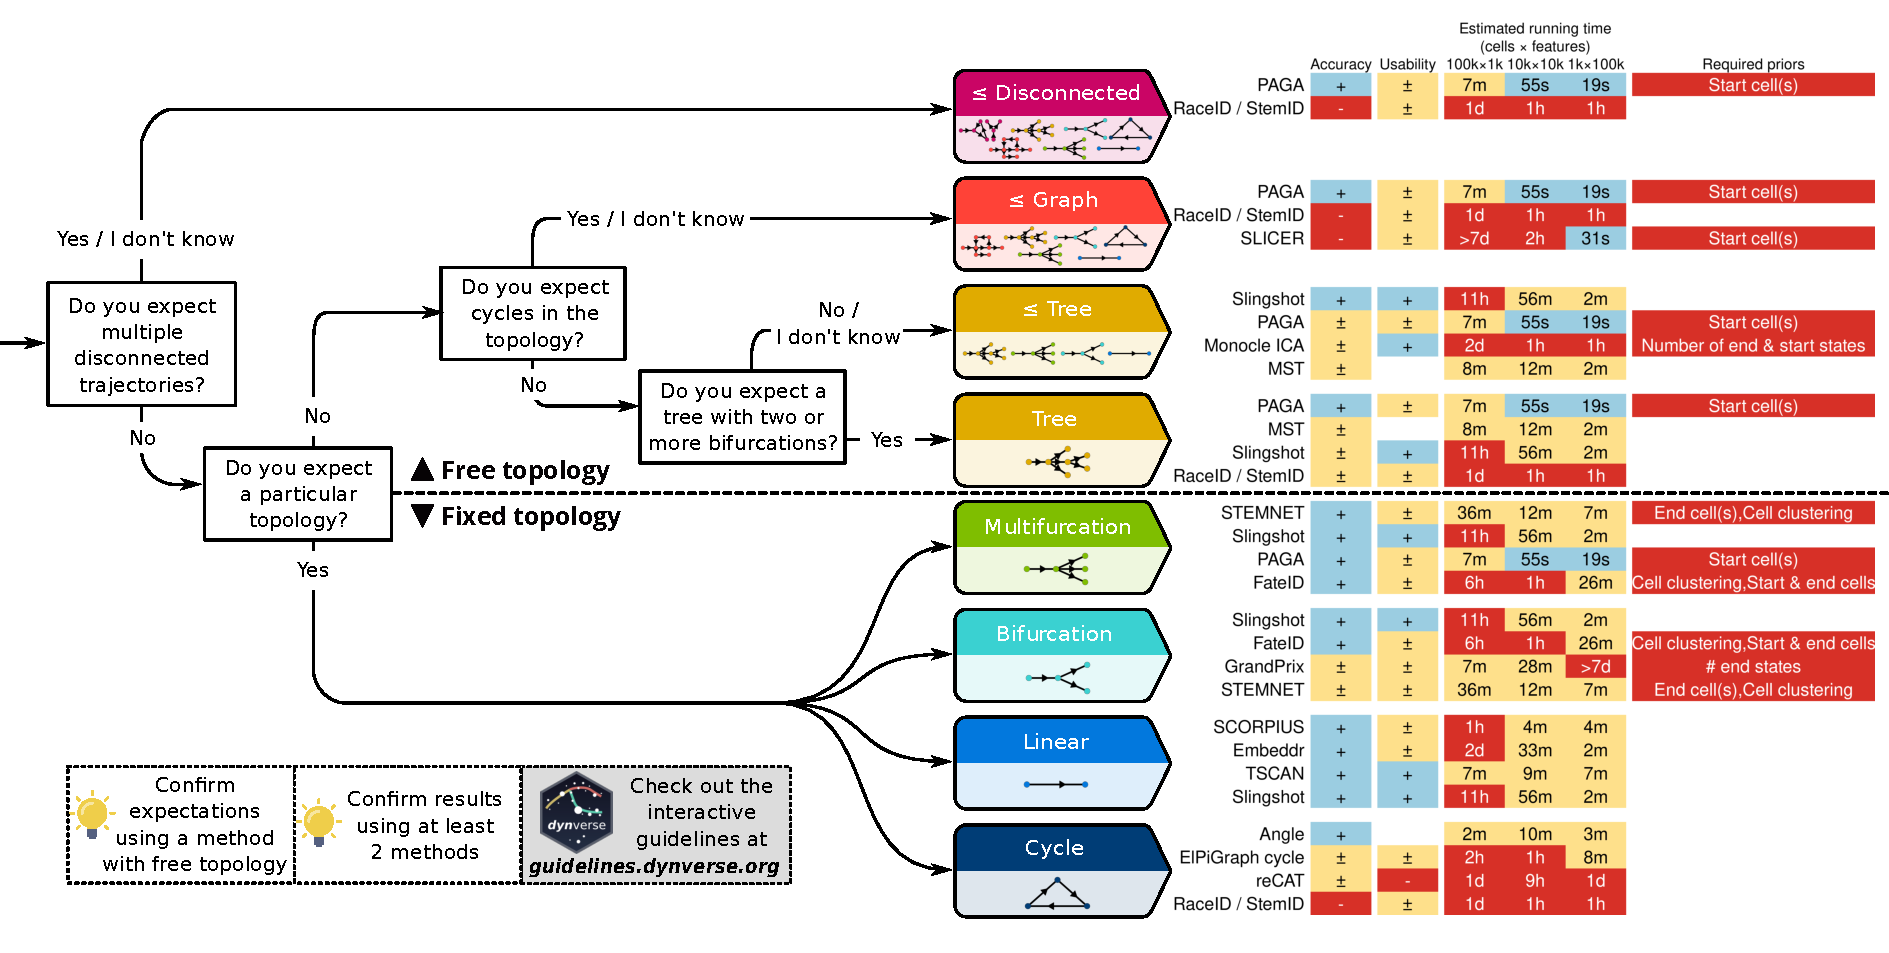
\includegraphics[width=\linewidth]{fig/figure_5.pdf}
	\caption{
		\textbf{Practical guidelines for method users.}
		As the performance of a method mostly depends on the topology of the trajectory, the choice of TI method will be primarily influenced by the user’s existing knowledge about the expected topology in the data. We therefore devised a set of practical guidelines, which combines the method’s performance, user friendliness and the number of assumptions a user is willing to make about the topology of the trajectory. Methods to the right are ranked according to their performance on a particular (set of) trajectory type. Further to the right are shown the accuracy (+: scaled performance $\geq$ 0.9, $\pm$: >0.6), usability scores (+:$\geq$0.9, $\pm$ $\geq$0.6), estimated running times and required prior information. k, thousands; m, millions.
	}
	\label{fig:figure_5}
\end{figure}

When inferring a trajectory on a dataset of interest, it is important to take two further points into account. First, it is critical that a trajectory, and the downstream results and/or hypotheses originating from it, are confirmed by multiple TI methods. This is to make sure that the prediction is not biased due to the given parameter setting or the particular algorithm underlying a TI method. The value of using different methods is further supported by our analysis indicating substantial complementarity between the different methods. Second, even if the expected topology is known, it can be beneficial to also try out methods that make less assumptions about the trajectory topology. When the expected topology is confirmed using such a method, it provides additional evidence to the user. When a more complex topology is produced, this could indicate that the underlying biology is much more complex than anticipated by the user.

Critical to the broad applicability of TI methods is the standardization of the input and output interfaces of TI methods, so that users can effortlessly execute TI methods on their dataset of interest, compare different predicted trajectories and apply downstream analyses, such as finding genes important for the trajectory, network inference \cite{aibar_scenicsinglecellregulatory_2017} or finding modules of genes \cite{saelens_comprehensiveevaluationmodule_2018}. Our framework is an initial attempt at tackling this problem, and we illustrate its usefulness here by comparing the predicted trajectories of several top-performing methods on datasets containing a linear, tree, cyclic and disconnected graph topology (Figure \ref{fig:figure_6}). Using our framework, this figure can be recreated using only a couple of lines of R code (\url{https://methods.dynverse.org}). In the future, this framework could be extended to allow additional input data, such as spatial and RNA velocity information \cite{lamanno_rnavelocitysingle_2018}, and easier downstream analyses. In addition, further discussion within the field is required to arrive at a consensus concerning a common interface for trajectory models, which can include additional features such as uncertainty and gene importance.

\begin{figure}[tbh!]
	\centering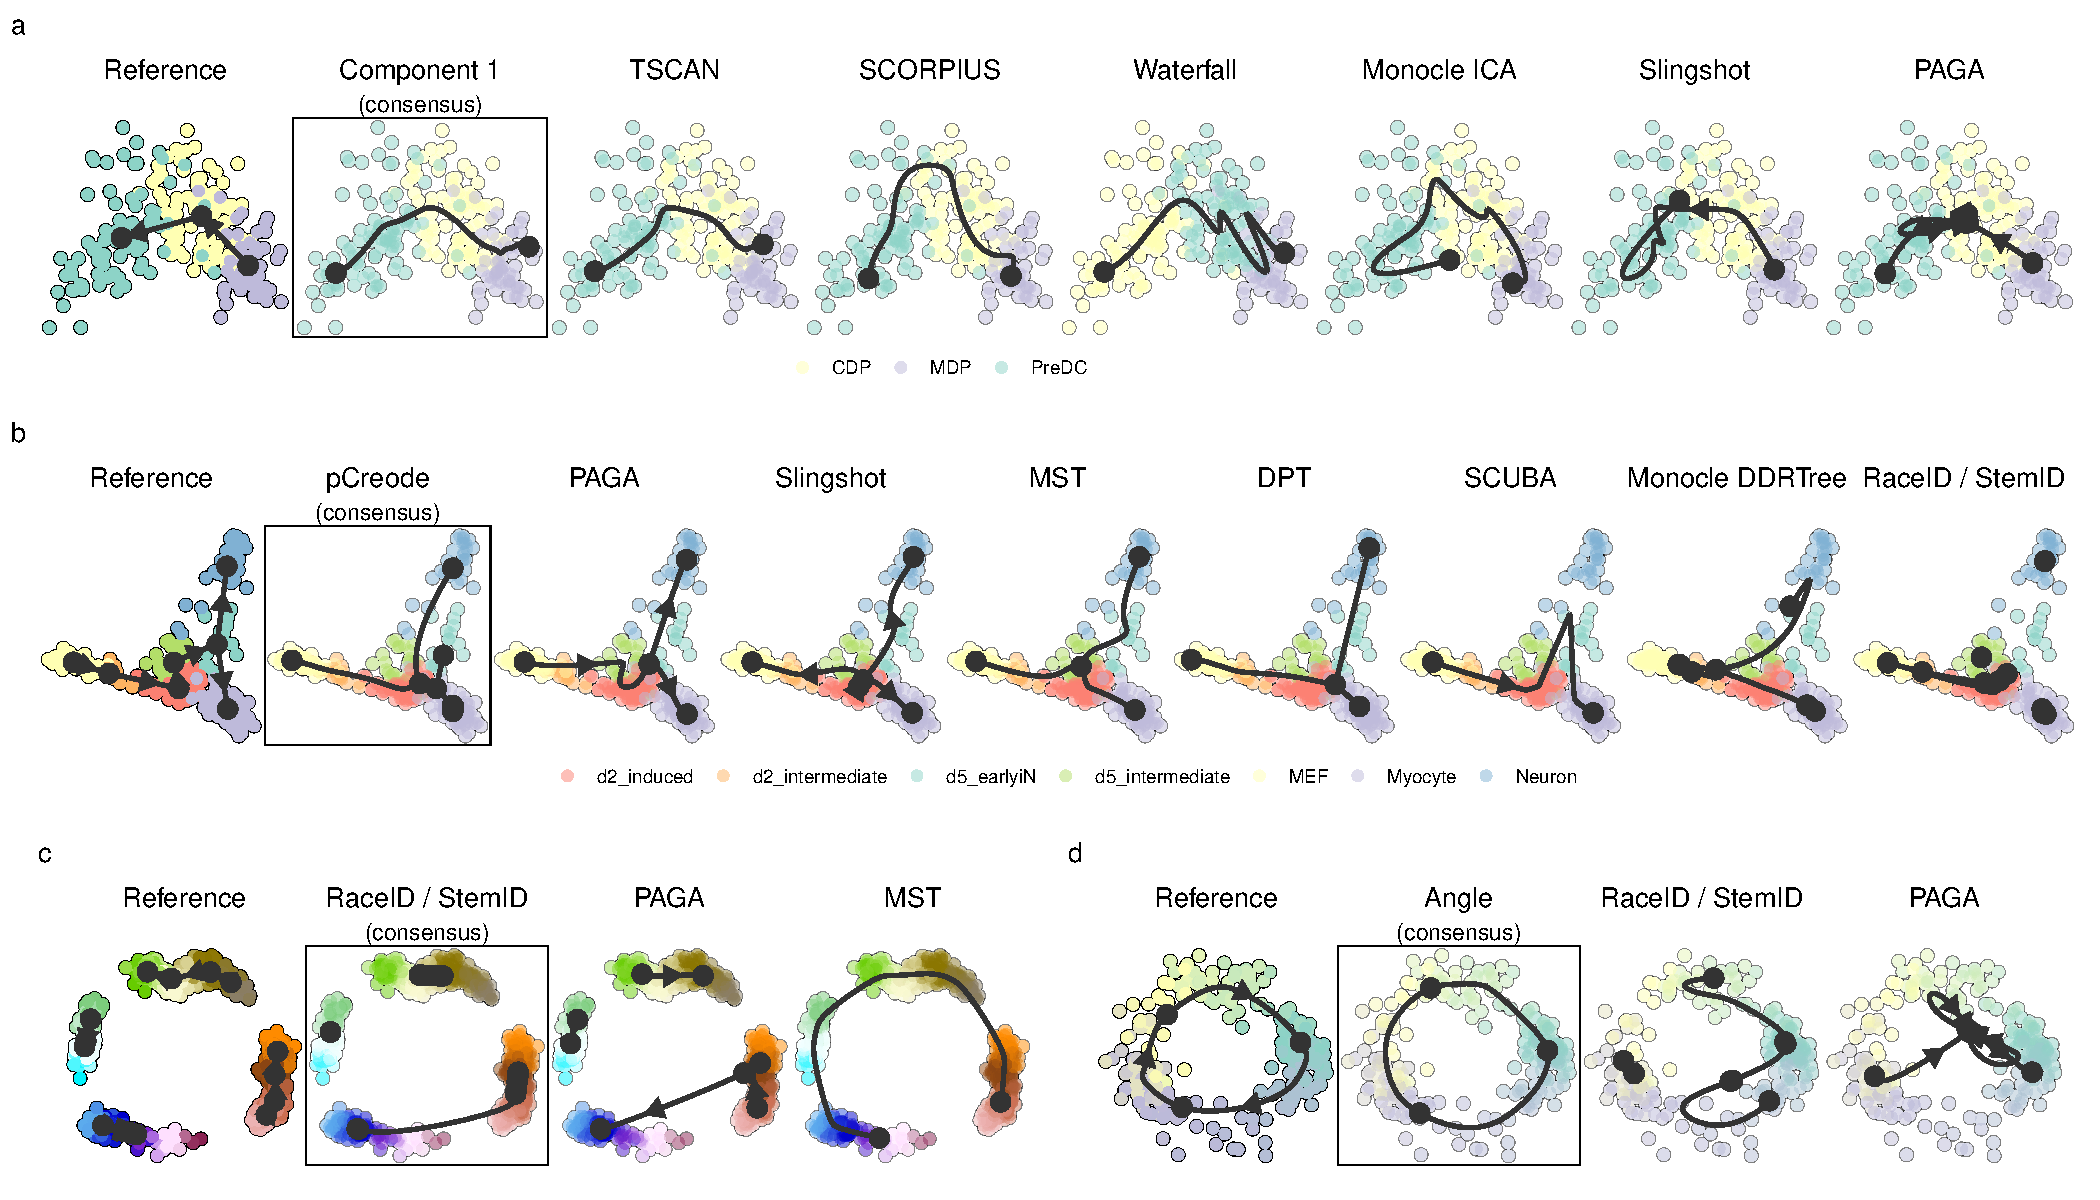
\includegraphics[width=\linewidth]{fig/figure_6.pdf}
	\caption{
		\textbf{Demonstration of how a common framework for TI methods facilitates broad applicability using some example datasets.}
		Trajectories inferred by each method were projected to a common dimensionality reduction using multidimensional scaling. For each dataset, we also calculated a ‘consensus’ prediction, by calculating the cordist between each pair of models and picking the model with the highest score on average. \textbf{a}, The top methods applied on a dataset containing a linear trajectory of differentiation dendritic cells, going from MDP, CDP to PreDC. \textbf{b}, The top methods applied on a dataset containing a bifurcating trajectory of reprogrammed fibroblasts. \textbf{c}, A synthetic dataset generated by dyntoy, containing four disconnected trajectories. \textbf{d}, A synthetic dataset generated by dyngen, containing a cyclic trajectory.
	}
	\label{fig:figure_6}
\end{figure}

Our study indicates that the field of trajectory inference is maturing, primarily for linear and bifurcating trajectories (Figure \ref{fig:figure_6}a,b). However, we also highlight several ongoing challenges, which should be addressed before TI can be a reliable tool for analyzing single-cell omics datasets with complex trajectories. Foremost, new methods should focus on improving the unbiased inference of tree, cyclic graph and disconnected topologies, as we found that methods repeatedly overestimate or underestimate the complexity of the underlying topology, even if the trajectory could easily be identified using a dimensionality reduction method (Figure \ref{fig:figure_6}c,d). Furthermore, higher standards for code assurance and documentation could help in adopting these tools across the single-cell omics field. Finally, new tools should be designed to scale well with the increasing number of cells and features. We found that only a handful of current methods can handle datasets with more than 10,000 cells within a reasonable time frame. To support the development of these new tools, we provide a series of vignettes on how to wrap and evaluate a method on the different measures proposed in this study at \url{https://benchmark.dynverse.org}.

We found that the performance of a method can be very variable between datasets, and therefore included a large set of both real and synthetic data within our evaluation, leading to a robust overall ranking of the different methods. However, ‘good-yet-not-the-best’ methods \cite{norel_selfassessmenttrapcan_2011} can still provide a very valuable contribution to the field, especially if they make use of novel algorithms, return a more scalable solution or provide a unique insight in specific use cases. This is also supported by our analysis of method complementarity. Some examples for the latter include PhenoPath, which can include additional covariates in its model, ouija, which returns a measure of uncertainty of each cell’s position within the trajectory, and StemID, which can infer the directionality of edges within the trajectory.


\section{Methods}

\subsection{Trajectory inference methods}

We gathered a list of 71 trajectory inference tools (Supplementary Table~\hyperref[tab:supptable_1]{3.1}) by searching the literature for ‘trajectory inference’ and ‘pseudotemporal ordering’, and based on two existing lists found online: \href{https://github.com/seandavi/awesome-single-cell}{awesome-single-cell} \cite{davis_awesomesinglecell_2018} and \href{https://github.com/agitter/single-cell-pseudotime}{single-cell-pseudotime} \cite{gitter_singlecellrnaseqpseudotime_2018}. We welcome any contributions by creating an issue at \href{https://methods.dynverse.org}{https://methods.dynverse.org}.

Methods were excluded from the evaluation based on several criteria: (1) not freely available; (2) no code available; (3) superseded by another method; (4) requires data types other than expression; (5) no programming interface; (6) unresolved errors during wrapping; (7) too slow (requires more than 1 h on a 100 $\times$ 100 dataset); (8) does not return an ordering; and (9) requires additional user input during the algorithm (other than prior information). The discussions on why these methods were excluded can be found at \url{https://github.com/dynverse/dynmethods/issues?q=label:unwrappable}. In the end, we included 45 methods in the evaluation.


\subsection{Method wrappers}

To make it easy to run each method in a reproducible manner, each method was wrapped within Docker and Singularity containers (available at \url{https://methods.dynverse.org}). These containers are automatically built and tested using Travis continuous integration (\url{https://travis-ci.org/dynverse}) and can be ran using both Docker and Singularity. For each method, we wrote a wrapper script based on example scripts or tutorials provided by the authors (as mentioned in the respective wrapper scripts). This script reads in the input data, runs the method and outputs the files required to construct a trajectory. We also created a script to generate an example dataset, which is used for automated testing.

We used the GitHub issues system to contact the authors of each method, and asked for feedback on the wrappers, the metadata and the usability scores. About one-third of the authors responded and we improved the wrappers based on their feedback. These discussions can be viewed on GitHub: \url{https://github.com/dynverse/dynmethods/issues?q=label:method_discussion}

\subsubsection{Method input}

As input, we provided each method with either the raw count data (after cell and gene filtering) or normalized expression values, based on the description in the method documentation or from the study describing the method. A large portion of the methods requires some form of prior information (for example, a start cell) to be executable. Other methods optionally allow the exploitation of certain prior information. Prior information can be supplied as a starting cell from which the trajectory will originate, a set of important marker genes or even a grouping of cells into cell states. Providing prior information to a TI method can be both a blessing and a curse. In one way, prior information can help the method to find the correct trajectory among many, equally likely, alternatives. On the other hand, incorrect or noisy prior information can bias the trajectory towards current knowledge. Moreover, prior information is not always easily available, and its subjectivity can therefore lead to multiple equally plausible solutions, restricting the applicability of such TI methods to well-studied systems.


The prior information was extracted from the reference trajectory as follows:

\begin{itemize}
	\item \textbf{Start cells}: the identity of one or more start cells. For both real and synthetic data, a cell was chosen that was the closest (in geodesic distance) to each milestone with only outgoing edges. For ties, one random cell was chosen. For cyclic datasets, a random cell was chosen.
	\item \textbf{End cells}: the identity of one or more end cells. This is similar to the start cells, but now for every state with only incoming edges.
	\item \textbf{No. of end states}: number of terminal states, i.e., the number of milestones with only incoming edges.
	\item \textbf{Grouping}: for each cell a label showing which state/cluster/branch it belongs to. For real data, the states were from the gold/silver standard. For synthetic data, each milestone was seen as one group and cells were assigned to their closest milestone.
	\item \textbf{No. of branches}: number of branches/intermediate states. For real data, this was the number of states in the gold/silver standard. For synthetic data, this was the number of milestones.
	\item \textbf{Discrete time course}: for each cell a time point from which it was sampled. If available, this was directly extracted from the reference trajectory; otherwise the geodesic distance from the root milestone was used. For synthetic data, the simulation time was uniformly discretised into four timepoints.
	\item \textbf{Continuous time course}: for each cell a time point from which it was sampled. For real data, this was equal to the discrete time course. For synthetic data, we used the internal simulation time of each simulator.
\end{itemize}



\subsubsection{Common trajectory model}

Due to the absence of a common format for trajectory models, most methods return a unique set of output formats with few overlaps. We therefore post-processed the output of each method into a common probabilistic trajectory model (Figure \ref{fig:supfigure_1}a). This model consisted of three parts. (1) The milestone network represents the overall network topology, and contains edges between different milestones and the length of the edge between them. (2) The milestone percentages contain, for each cell, its position between milestones and sums for each cell to one. (3) The regions of delayed commitment define connections between three or more milestones. These must be explicitly defined in the trajectory model and per region one milestone must be directly connected to all other milestones of the region.

Depending on the output of a method, we used different strategies to convert the output to our model (Figure \ref{fig:supfigure_1}b). Special conversions are denoted by an asterisk (*) and will be explained in more detail in the second list below.



\begin{itemize}
	\item \textbf{Type 1, direct}: CALISTA*, DPT*, ElPiGraph, ElPiGraph cycle, ElPiGraph linear, MERLoT, PAGA, SLICE*, Slingshot, URD* and Wishbone. The wrapped method directly returned a network of milestones, the regions of delayed commitment and for each cell it is given to what extent it belongs to a milestone. In some cases, this indicates that additional transformations were required for the method, not covered by any of the following output formats. Some methods returned a branch network instead of a milestone network and this network was converted by calculating the line graph of the branch network.
	\item \textbf{Type 2, linear pseudotime}: Component 1, Embeddr, FORKS, MATCHER, ouija, ouijaflow, PhenoPath, pseudogp, SCIMITAR, SCORPIUS, topslam, TSCAN, Wanderlust and Waterfall. The method returned a pseudotime, which is translated into a linear trajectory where the milestone network contains two milestones and cells are positioned between these two milestones.
	\item \textbf{Type 3, cyclical pseudotime}: Angle and reCAT. The method returned a pseudotime, which is translated into a cyclical trajectory where the milestone network contains three milestones and cells are positioned between these three milestones. These milestones were positioned at pseudotime 0, 1/3 and 2/3.
	\item \textbf{Type 4, end state probability}: FateID, GPfates, GrandPrix, MFA*, SCOUP and STEMNET. The method returned a pseudotime and for each cell and end state a probability (Pr) for how likely a cell will end up in a certain end state. This was translated into a star-shaped milestone network, with one starting milestone (M0) and several outer milestones (Mi), with regions of delayed commitment between all milestones. The milestone percentage of a cell to one of the outer milestones was equal to pseudotime$\times$PrMi. The milestone percentage to the starting milestone was equal to 1 $-$ pseudotime.
	\item \textbf{Type 5, cluster assignment}: Mpath and SCUBA. The method returned a milestone network and an assignment of each cell to a specific milestone. Cells were positioned onto the milestones they are assigned to, with milestone percentage equal to 1.
	\item \textbf{Type 6, orthogonal projection}: MST, pCreode and RaceID/StemID. The method returned a milestone network, and a dimensionality reduction of the cells and milestones. The cells were projected to the closest nearest segment, thus determining the cells’ position along the milestone network. If a method also returned a cluster assignment (type 5), we limited the projection of each cell to the closest edge connecting to the milestone of a cell. For these methods, we usually wrote two wrappers, one which included the projection and one without.
	\item\textbf{ Type 7, cell graph}: CellRouter, CellTrails, cellTree Gibbs, cellTree maptpx, cellTree VEM, Monocle DDRTree, Monocle ICA, Sincell* and SLICER. The method returned a network of cells and which cell–cell transitions were part of the ‘backbone’ structure. Backbone cells with degree $\neq$ 2 were regarded as milestones and all other cells were placed on transitions between the milestones. If a method did not return a distance between pairs of cells, the cells were uniformly positioned between the two milestones. Otherwise, we first calculated the distance between two milestones as the sum of the distances between the cells and then divided the distance of each pair of cells with the total distance to get the milestone percentages.
\end{itemize}


Special conversions were necessary for certain methods:


\begin{itemize}
	\item \textbf{CALISTA}: We assigned the cells to the branch at which the sum of the cluster probabilities of two connected milestones was the highest. The cluster probabilities of the two selected milestones were then used as milestone percentages. This was then processed as a type 1, direct, method.
	\item \textbf{DPT}: We projected the cells onto the cluster network, consisting of a central milestone (this cluster contained the cells that were assigned to the ‘unknown’ branch) and three terminal milestones, each corresponding to a tip point. This was then processed as a type 1, direct, method.
	\item \textbf{Sincell}: To constrain the number of milestones this method creates, we merged two cell clusters iteratively until the percentage of leaf nodes was below a certain cutoff, with the default cutoff set to 25$\%$. This was then processed as a type 7, cell graph, method.
	\item \textbf{SLICE}: As discussed in the vignette of SLICE (\url{https://research.cchmc.org/pbge/slice.html}), we ran principal curves one by one for every edge detected by SLICE. This was then processed as a type 1, direct, method.
	\item \textbf{MFA}: We used the branch assignment as state probabilities, which together with the global pseudotime were processed as a type 4, end state probabilities, method.
	\item \textbf{URD}: We extracted the pseudotime of a cell within each branch using the y positions in the tree layout. This was then further processed as a type 1, direct, method.
	
\end{itemize}



More information on how each method was wrapped can be found within the comments of each wrapper script, listed at \url{https://methods.dynverse.org}.

\subsubsection{Off-the-shelf methods}

For baseline performance, we added several ‘off-the-shelf’ TI methods that can be run using a few lines of code in R.

\begin{itemize}
	
	\item \textbf{Component 1}: This method returns the first component of a principal component analysis (PCA) dimensionality reduction as a linear trajectory. This method is especially relevant as it has been used in a few studies already \cite{kouno_temporaldynamicstranscriptional_2013,zeng_pseudotemporalorderingsingle_2017}.
	
	\item \textbf{Angle}: Similar to the previous method, this method computes the angle with respect to the origin in a two-dimensional PCA and uses this angle as a pseudotime for generating a cyclical trajectory.
	
	\item \textbf{MST}: This method performs PCA dimensionality reduction, followed by clustering using the R mclust package, after which the clusters are connected using a minimum spanning tree. The trees are orthogonally projected to the nearest segment of the tree. This baseline is highly relevant as many methods follow the same methodology: dimensionality reduction, clustering, topology inference and project cells to topology.
	
\end{itemize}

\subsection{Trajectory types}

We classified all possible trajectory topologies into distinct trajectory types, based on topological criteria (Figure \ref{fig:figure_1}c). These trajectory types start from the most general trajectory type, a disconnected graph, and move down (within a directed acyclic graph structure), progressively becoming more simple until the two basic types are reached: linear and cyclical. A disconnected graph is a graph in which only one edge can exist between two nodes. A (connected) graph is a disconnected graph in which all nodes are connected. An acyclic graph is a graph containing no cycles. A tree is an acyclic graph containing no convergences (no nodes with in-degree higher than 1). A convergence is an acyclic graph in which only one node has a degree larger than 1 and this same node has an in-degree of 1. A multifurcation is a tree in which only one node has a degree larger than 1. A bifurcation is a multifurcation in which only one node has a degree equal to 3. A linear topology is a graph in which no node has a degree larger than 3. Finally, a cycle is a connected graph in which every node has a degree equal to 2. In most cases, a method that was able to detect a complex trajectory type was also able to detect less complex trajectory types, with some exceptions shown in Figure \ref{fig:figure_2}a.

For simplicity, we merged the bifurcation and convergence trajectory type, and the acyclic graph and connected graph trajectory type in the main figures of the paper.


\subsection{Real datasets}

We gathered real datasets by searching for ‘single-cell’ at the Gene Expression Omnibus and selecting those datasets in which the cells are sampled from different stages in a dynamic process (Supplementary Table~\hyperref[tab:supptable_2]{3.2}). The scripts to download and process these datasets are available on our repository (\url{https://benchmark.dynverse.org/tree/master/scripts/01-datasets}). Whenever possible, we preferred to start from the raw counts data. These raw counts were all normalized and filtered using a common pipeline, as discussed later. Some original datasets contained more than one trajectory, in which case we split the dataset into its separate connected trajectory, but also generated several combinations of connected trajectories to include some datasets with disconnected trajectories in the evaluation. In the end, we included 110 datasets for this evaluation.

For each dataset, we extracted a reference trajectory, consisting of two parts: the cellular grouping (milestones) and the connections between these groups (milestone network). The cellular grouping was provided by the authors of the original study, and we classified it as a gold standard when it was created independently from the expression matrix (such as from cell sorting, the origin of the sample, the time it was sampled or cellular mixing) or as a silver standard otherwise (usually by clustering the expression values). To connect these cell groups, we used the original study to determine the network that the authors validated or otherwise found to be the most likely. In the end, each group of cells was placed on a milestone, having a percentage of 1 for that particular milestone. The known connections between these groups were used to construct the milestone network. If there was biological or experimental time data available, we used this as the length of the edge; otherwise we set all the lengths equal to one.

\subsection{Synthetic datasets}

To generate synthetic datasets, we used four different synthetic data simulators:

\begin{itemize}
	\item \textbf{dyngen}: simulations of gene regulatory networks, available at \url{https://github.com/dynverse/dyngen}
	\item \textbf{dyntoy}: random gradients of expression in the reduced space, available at \url{https://github.com/dynverse/dyntoy}
	\item \textbf{PROSSTT}: expression is sampled from a linear model that depends on pseudotime \cite{papadopoulos_prossttprobabilisticsimulation_2018}
	\item \textbf{Splatter}: simulations of non-linear paths between different expression states \cite{zappia_splattersimulationsinglecell_2017}
\end{itemize}


For every simulator, we took great care to make the datasets as realistic as possible. To do this, we extracted several parameters from all real datasets. We calculated the number of differentially expressed features within a trajectory using a two-way Mann–Whitney U test between every pair of cell groups. These values were corrected for multiple testing using the Benjamini-Hochberg procedure (FDR < 0.05) and we required that a gene was expressed in at least 5$\%$ of cells, and had at least a fold-change of 2. We also calculated several other parameters, such as drop-out rates and library sizes using the Splatter package \cite{zappia_splattersimulationsinglecell_2017}. These parameters were then given to the simulators when applicable, as described for each simulator below. Not every real dataset was selected to serve as a reference for a synthetic dataset. Instead, we chose a set of ten distinct reference real datasets by clustering all the parameters of each real dataset, and used the reference real datasets at the cluster centers from a pam clustering (with $k = 10$, implemented in the R cluster package) to generate synthetic data.

\subsubsection{dyngen}

The dyngen (Chapter~\ref{chap:dyngen}) workflow to generate synthetic data is based on the well established workflow used in the evaluation of network inference methods \cite{schaffter_genenetweaversilicobenchmark_2011,marbach_wisdomcrowdsrobust_2012} and consists of four main steps: network generation, simulation, gold standard extraction and simulation of the scRNA-seq experiment. At every step, we tried to mirror real regulatory networks, while keeping the model simple and easily extendible We simulated a total of 110 datasets, with 11 different topologies. 

\subsubsection{dyntoy}

For more simplistic data generation ("toy" datasets), we created the dyntoy workflow (\url{https://github.com/dynverse/dyntoy}). We created 12 topology generators (described below), and with 10 datasets per generator, this lead to a total of 120 datasets.

We created a set of topology generators, were $B(n, p)$ denotes a binomial distribution, and $U(a, b)$ denotes a uniform distribution:

\begin{itemize}
	\item Linear and cyclic, with number of milestones $\sim B(10, 0.25)$
	\item Bifurcating and converging, with four milestones
	\item Binary tree, with number of branching points $\sim U(3, 6)$
	\item Tree, with number of branching points $\sim U(3, 6)$ and maximal degree $\sim U(3, 6)$
\end{itemize} 

For more complex topologies we first calculated a random number of "modifications" $\sim U(3, 6)$ and a $\textit{deg}_{\textit{max}} \sim B(10, 0.25) + 1$. For each type of topology, we defined what kind of modifications are possible: divergences, loops, convergences and divergence-convergence. We then iteratively constructed the topology by uniformly sampling from the set of possible modifications, and adding this modification to the existing topology. For a divergence, we connected an existing milestone to a number of a new milestones. Conversely, for a convergence we connected a number of new nodes to an existing node. For a loop, we connected two existing milestones with a number of milestones in between. Finally for a divergence-convergence we connected an existing milestone to several new milestones which again converged on a new milestone. The number of nodes was sampled from $\sim B(\textit{deg}_{\textit{max}} - 3, 0.25) + 2$

\begin{itemize}
	\item Looping, allowed loop modifications
	\item Diverging-converging, allowed divergence and converging modifications
	\item Diverging with loops, allowed divergence and loop modifications
	\item Multiple looping, allowed looping modifications
	\item Connected, allowed looping, divergence and convergence modifications
	\item Disconnected, number of components sampled from $\sim B(5, 0.25) + 2$, for each component we randomly chose a topology from the ones listed above
\end{itemize}

After generating the topology, we sampled the length of each edge $\sim U(0.5, 1)$. We added regions of delayed commitment to a divergence in a random half of the cases. We then placed the number of cells (same number as from the reference real dataset), on this topology uniformly, based on the length of the edges in the milestone network.

For each gene (same number as from the reference real dataset), we calculated the Kamada-Kawai layout in 2 dimensions, with edge weight equal to the length of the edge. For this gene, we then extracted for each cell a density value using a bivariate normal distribution with $\mu \sim U(x_{\textit{min}}, x_{\textit{min}})$ and $\sigma \sim U(x_{\textit{min}}/10, x_{\textit{min}}/8)$. We used this density as input for a zero-inflated negative binomial distribution with $\mu ~ U(100, 1000) \times \textit{density}$, $k ~ U(\mu / 10, \mu / 4)$ and $pi$ from the parameters of the reference real dataset, to get the final count values.

This count matrix was then filtered and normalised using the pipeline described below.

\subsubsection{PROSSTT}

PROSSTT is a recent data simulator \cite{papadopoulos_prossttprobabilisticsimulation_2018}, which simulates expression using linear mixtures of expression programs and random walks through the trajectory. We used 5 topology generators from dyntoy (linear, bifurcating, multifurcating, binary tree and tree), and simulated for each topology generator 10 datasets using different reference real datasets. However, due to frequent crashes of the tool, only 19 datasets created output and were thus used in the evaluation.

Using the simulate\_lineage function, we simulated the lineage expression, with parameters $a \sim U(0.01, 0.1)$, $\textit{branch-tol}_{\textit{intra}} \sim U(0, 0.9)$ and $\textit{branch-tol}_{\textit{inter}} \sim U(0, 0.9)$. These parameter distributions were chosen very broad so as to make sure both easy and difficult datasets are simulated. After simulating base gene expression with simulate\_base\_gene\_exp, we used the sample\_density function to finally simulate expression values of a number of cells (the same as from the reference real dataset), with $\alpha \sim \textit{Lognormal}$ ($\mu = 0.3$ and $\sigma = 1.5$) and $\beta \sim \textit{Lognormal}$ ($\mu = 2$ and $\sigma = 1.5$). Each of these parameters were centred around the default values of PROSSTT, but with enough variability to ensure a varied set of datasets.

This count matrix was then filtered and normalised using the pipeline described below.

\subsubsection{Splatter}

Splatter \cite{zappia_splattersimulationsinglecell_2017} simulates expression values by constructing non-linear paths between different states, each having a distinct expression profile. We used 5 topology generators from dyntoy (linear, bifurcating, multifurcating, binary tree and tree), and simulated for each topology generator 10 datasets using different reference real datasets, leading to a total of 50 datasets.

We used the splatSimulatePaths function from Splatter to simulate datasets, with number of cells and genes equal to those in the reference real dataset, and with parameters  $\textit{nonlinearProb}$, $\textit{sigmaFac}$ and $\textit{skew}$ all sampled from $U(0, 1)$.

\subsection{Dataset filtering and normalization}

We used a standard single-cell RNA-seq preprocessing pipeline that applies parts of the scran and scater Bioconductor packages \cite{lun_stepbystepworkflowlowlevel_2016}. The advantages of this pipeline are that it works both with and without spike-ins, and it includes a harsh cell filtering that looks at abnormalities in library sizes, mitochondrial gene expression and the number of genes expressed using median absolute deviations (which we set to 3). We required that a gene was expressed in at least 5$\%$ of the cells and that it should have an average expression higher than 0.02. Furthermore, we used the pipeline to select the most highly variable genes, using a false discovery rate of 5$\%$ and a biological component higher than 0.5. As a final filter, we removed both all-zero genes and cells until convergence.

\subsection{Benchmark metrics}

The importance of using multiple metrics to compare complex models has been stated repeatedly \cite{norel_selfassessmenttrapcan_2011}. Furthermore, a trajectory is a model with multiple layers of complexity, which calls for several metrics each assessing a different layer. We therefore defined several possible metrics for comparing trajectories, each investigating different layers. These are all discussed in Section~\ref{sec:dynb_supn1} along with examples and robustness analyses when appropriate.

Next, we created a set of rules to which we think a good trajectory metric should conform, and tested this empirically for each metric by comparing scores before and after perturbing a dataset (Section~\ref{sec:dynb_supn1}). Based on this analysis, we chose four metrics for the evaluation, each assessing a different aspect of the trajectory: (1) the HIM measures the topological similarity; (2) the F1branches compares the branch assignment; (3) the cordist assesses the similarity in pairwise cell–cell distances and thus the cellular positions; and (4) the wcorfeatures looks at whether similar important features (genes) are found in both the reference dataset and the prediction.

\subsubsection{The Hamming–Ipsen–Mikhailov metric}

The HIM metric \cite{jurman_himglocalmetric_2015} uses the two weighted adjacency matrices of the milestone networks as input (weighted by edge length). It is a linear combination of the normalized Hamming distance, which gives an indication of the differences in edge lengths, and the normalized Ipsen–Mikhailov distance, which assesses the similarity in degree distributions. The latter has a parameter $\gamma$, which was fixed at 0.1 to make the scores comparable between datasets. We illustrate the metric and discuss alternatives in Section~\ref{sec:dynb_supn1}.

\subsubsection{The F1 between branch assignments}

To compare branch assignment, we used an F1 score, also used used for comparing biclustering methods \cite{saelens_comprehensiveevaluationmodule_2018}. To calculate this metric, we first calculated the similarity of all pairs of branches between the two trajectories using the Jaccard similarity. Next, we defined the ‘Recovery' (respectively ‘Relevance') as the average maximal similarity of all branches in the reference dataset (respectively prediction). The F1branches was then defined as the harmonic mean between Recovery and Relevance. We illustrate this metric further in Section~\ref{sec:dynb_supn1}.

\subsubsection{Correlation between geodesic distances}

When the position of a cell is the same in both the reference and the prediction, its relative distances to all other cells in the trajectory should also be the same. This observation is the basis for the cordist metric. To calculate the cordist, we first sampled 100 waypoint cells in both the prediction and the reference dataset, using stratified sampling between the different milestones, edges and regions of delayed commitment, weighted by the number of cells in each collection. We then calculated the geodesic distances between the union of waypoint cells from both datasets and all other cells. The calculation of the geodesic distance depended on the location of the two cells within the trajectory, further discussed in Section~\ref{sec:dynb_supn1}, and was weighted by the length of the edge in the milestone network. Finally, the cordist was defined as the Spearman rank correlation between the distances of both datasets. We illustrate the metric and assess the effect of the number of waypoint cells in Section~\ref{sec:dynb_supn1}.

\subsubsection{The correlation between important features}

The wcorfeatures assesses whether the same differentially expressed features are found using the predicted trajectory as in the known trajectory. To calculate this metric, we used Random Forest regression (implemented in the R ranger package \cite{wright_rangerfastimplementation_2017}), to predict expression values of each gene, based on the geodesic distances of a cell to each milestone. We then extracted feature importance values for each feature and calculated the similarity of the feature importances using a weighted Pearson correlation, weighted by the feature importance in the reference dataset to give more weight to large differences. As hyperparameters we set the number of trees to 10,000 and the number of features on which to split to 1$\%$ of all available features. We illustrate this metric and assess the effect of its hyperparameters in Section~\ref{sec:dynb_supn1}.

\subsubsection{Score aggregation}

To rank methods, we needed to aggregate the different scores on two levels: across datasets and across different metrics. This aggregation strategy is explained in more detail in Section~\ref{sec:dynb_supn1}.

To ensure that easy and difficult datasets have equal influence on the final score, we first normalized the scores on each dataset across the different methods. We shifted and scaled the scores to $\sigma$ = 1 and $\mu$ = 0, and then applied the unit probability density function of a normal distribution on these values to get the scores back into the [0,1] range.

Since there is a bias in dataset source and trajectory type (for example, there are many more linear datasets), we aggregated the scores per method and dataset in multiple steps. We first aggregated the datasets with the same dataset source and trajectory type using an arithmetic mean of their scores. Next, the scores were averaged over different dataset sources, using an arithmetic mean that was weighted based on how much the synthetic and silver scores correlated with the real gold scores. Finally, the scores were aggregated over the different trajectory types again using an arithmetic mean.

Finally, to get an overall benchmarking score, we aggregated the different metrics using a geometric mean.

\subsection{Method execution}

Each execution of a method on a dataset was performed in a separate task as part of a gridengine job. Each task was allocated one CPU core of an Intel(R) Xeon(R) CPU E5-2665 at 2.40 GHz, and one R session was started for each task. During the execution of a method on a dataset, if the time limit (>1 h) or memory limit (16 GB) was exceeded, or an error was produced, a zero score was returned for that execution.

\subsection{Complementarity}

To assess the complementarity between different methods, we first calculated for every method and dataset whether the overall score was equal to or higher than 95$\%$ of the best overall score for that particular dataset. We then calculated for every method the weighted percentage of datasets that fulfilled this rule, weighted similarly as in the benchmark aggregation, and chose the best method. We iteratively added new methods until all methods were selected. For this analysis, we did not include any methods that require any strong prior information and only included methods that could detect the trajectory types present in at least one of the datasets.

\subsection{Scalability}

To assess the scalability of each method, we started from five real datasets, selected using the centers from a k-medoids as discussed before. We up- and downscaled these datasets between 10 and 100,000 cells and 10 and 100,000 features, while never going higher than 1,000,000 values in total. To generate new cells or features, we first generated a 10-nearest-neighbor graph of both the cells and features from the expression space. For every new cell or feature, we used a linear combination of one to three existing cells or features, where each cell or feature was given a weight sampled from a uniform distribution between 0 and 1.

We ran each method on each dataset for maximally 1 h and gave each process 10 GB of memory. To determine the running time of each method, we started the timer right after data loading and the loading of any packages, and stopped the clock before postprocessing and saving of the output. Pre- and postprocessing steps specific to a method, such as dimensionality reduction and gene filtering, were included in the time. To estimate the maximal memory usage, we used the max\_vmem value from the qacct command provided by a gridengine cluster. We acknowledge, however, that these memory estimates are very noisy and the averages provided in this study are therefore only rough estimates.

The relationship between the dimensions of a dataset and the running time or maximal memory usage was modeled using shape constrained additive models \cite{pya_shapeconstrainedadditive_2015}, with $log_{10}|\textit{cells}|$ and $log_{10}|\textit{features}|$ as predictor variables, and fitted this model using the scam function as implemented in the R scam package, with $log_{10}\textit{time}$ (or $log_{10}\textit{memory}$) as outcome.

To classify the time complexity of each method with respect to the number of cells, we predicted the running time at 10,000 features with increasing number of cells from 100 to 100,000, with steps of 100. We trained a generalized linear model with the following function: $y \approxeq \log{x} + \sqrt{x} + x + x^2 + x^3$ with y as running time and x as the number of cells or features. The time complexity of a method was then classified using the weights w from this model:

$$
\begin{cases}
\text{superquadratic} & \text{if } w_{x^3} > 0.25,\\
\text{quadratic} & \text{if } w_{x^2} > 0.25,\\
\text{linear} & \text{if } w_x > 0.25,\\
\text{sublinear} & \text{if } w_{\text{log}(x)} > 0.25 \text{ or } w_{\text{sqrt}(x)} > 0.25,\\
\text{case with highest weight} & \text{else.}
\end{cases}
$$

This process was repeated for classifying the time complexity with respect to the number of features, and the memory complexity both with respect to the number of cells and features.

\subsection{Stability}

In the ideal case, a method should produce a similar trajectory, even when the input data is slightly different. However, running the method multiple times on the same input data would not be the ideal approach to assess its stability, given that a lot of tools are artificially deterministic by internally resetting the pseudorandom number generator (for example, using the `set.seed` function in R or the `random.seed` function in numpy). To assess the stability of each method, we therefore selected a number of datasets, which consisted of 25$\%$ of the datasets accounting for 15$\%$ of the total runtime, chosen such that after aggregation the overall scores still has > 0.99 correlation with the original overall ranking. We subsampled each dataset 10 times with 95$\%$ of the original cells and 95$\%$ of the original features. We ran every method on each of the bootstraps, and assessed the stability by calculating the benchmarking scores between each pair of subsequent models (run $i$ is compared to run $i+1$). For the cordist and F1branches, we only used the intersection between the cells of two datasets, while the intersection of the features was used for the wcorfeatures.

\subsection{Usability}

We created a transparent scoring scheme to quantify the usability of each method based on several existing tool quality and programming guidelines in the literature and online (Table \ref{tab:scoresheet}). The main goal of this quality control is to stimulate the improvement of current methods, and the development of user- and developer-friendly new methods. The quality control assessed six categories, each looking at several aspects, which are further divided into individual items. The availability category checks whether the method is easily available, whether the code and dependencies can be easily installed, and how the method can be used. The code quality assesses the quality of the code both from a user perspective (function naming, dummy proofing and availability of plotting functions) and a developer perspective (consistent style and code duplication). The code assurance category is frequently overlooked, and checks for code testing, continuous integration \cite{beaulieu-jones_reproducibilitycomputationalworkflows_2017} and an active support system. The documentation category checks the quality of the documentation, both externally (tutorials and function documentation) and internally (inline documentation). The behavior category assesses the ease by which the method can be run, by looking for unexpected output files and messages, prior information and how easy the trajectory model can be extracted from the output. Finally, we also assessed certain aspects of the study in which the method was proposed, such as publication in a peer-reviewed journal, the number of datasets in which the usefulness of the method was shown and the scope of method evaluation in the paper.

Each quality aspect received a weight depending on how frequently it was found in several papers and online sources that discuss tool quality (Table \ref{tab:scoresheet}). This was to make sure that more important aspects, such as the open source availability of the method, outweighed other less important aspects, such as the availability of a graphical user interface. For each aspect, we also assigned a weight to the individual questions being investigated (Table \ref{tab:scoresheet}). For calculating the final score, we weighed each of the six categories equally.

\subsection{Guidelines}

For each set of outcomes in the guidelines figure, we selected one to four methods, by first filtering the methods on those that can detect all required trajectory types, and ordering the methods according to their average accuracy score on datasets containing these trajectory types (aggregated according to the scheme presented in the section Accuracy).

We used the same approach for selecting the best set of methods in the guidelines app (\url{http://guidelines.dynverse.org}), developed using the R shiny package. This app will also filter the methods, among other things, depending on the predicted running time and memory requirements, the prior information available and the preferred execution environment (using the dynmethods package or standalone).

\subsection{Reporting Summary}

Further information on research design is available in the Nature Research Reporting Summary, available at \url{https://www.nature.com/articles/s41587-019-0071-9\#MOESM2}.


\section{Supplementary Figures and Tables}

\paragraph{Supplementary Table 3.1: Overview of available trajectory inference tools, and whether they were included in	this study.} \label{tab:supptable_1}
Download link: \url{https://static-content.springer.com/esm/art\%3A10.1038\%2Fs41587-019-0071-9/MediaObjects/41587\_2019\_71\_MOESM3\_ESM.xlsx}.

\paragraph{Supplementary Table 3.2: Overview of the real datasets used in this study.} \label{tab:supptable_2}
Download link:
\url{https://static-content.springer.com/esm/art\%3A10.1038\%2Fs41587-019-0071-9/MediaObjects/41587\_2019\_71\_MOESM4\_ESM.xlsx}.


\paragraph{Supplementary Figure 3.1: Results from the evaluation, for all methods and across all evaluation criteria.} \label{fig:suppfig_2}
(a) We characterized the methods according to the wrapper type, their required priors, whether the inferred topology is constrained by the algorithm (fixed) or a parameter (param), and the types of inferable topologies. The methods are grouped vertically based on the most complex trajectory type the y can infer. (b) The overall results of the evaluation on four criteria: benchmarking using a reference trajectory on real and synthetic data, scalability with increasing number of cells and features, stability across dataset subsamples, and quality  of  the  implementation.  (c)  Accuracy  of  trajectory  inference  methods  across metrics,  dataset sources  and  dataset  trajectory types. The performance of a method is generally more stable across dataset sources, but very  variable depending on the metric and trajectory  type.  (d)  Predicted  execution  times  and memory  usage  for  varying  numbers  of  cells  and  features  (\# cells $\times$ \# features). Predictions were made by training a regression model after running each method on bootstrapped datasets with varying numbers of cells and features. (e) Stability results by calculating the average pairwise similarity between models inferred across multiple runs of the same method. (f) Usability scores of the tool and corresponding manuscript, grouped per category.
Download link: \url{https://github.com/dynverse/dynbenchmark_results/raw/master/08-summary/results_suppfig.pdf}.

\section{Supplementary Note 1: Metrics to compare two trajectories} \label{sec:dynb_supn1}

A trajectory, as defined in our evaluation, is a model with multiple abstractions. The top abstraction is the topology which contains information about the paths each cell can take from their starting point. Deeper abstractions involve the mapping of each cell to a particular branch within this network, and the position (or ordering) of each cells within these branches. Internally, the topology is represented by the milestone network and regions of delayed commitment, the branch assignment and cellular positions are represented by the milestone percentages (Figure \ref{fig:snote1fig_1}).

\begin{figure}[tbh!]
	\centering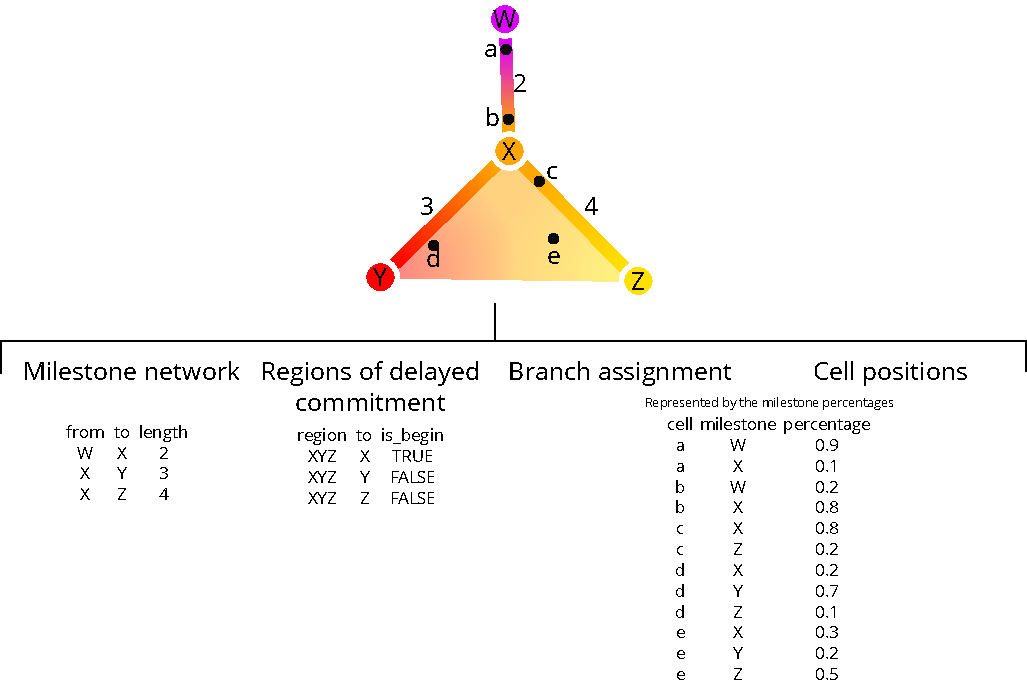
\includegraphics[width=\linewidth]{fig/snote1fig_1.pdf}
	\caption{
		\textbf{An example trajectory that will be used throughout this section.}
		It contains contains four milestones (W to Z) and five cells (a to e).
	}
	\label{fig:snote1fig_1}
\end{figure}

Given the multilayered complexity of a trajectory model, it is not trivial to compare the similarity of two trajectory models using only one metric. We therefore sought to use different comparison metrics, each serving a different purpose:

\begin{itemize}
	\item \textbf{Specific metrics} investigate one particular aspect of the trajectory. Such metrics make it possible to find particular weak points for methods, e.g. that a method is very good at ordering but does not frequently find the correct topology. Moreover, having multiple individual metrics allow personalised rankings of methods, for example for users which are primarily interested in using the method correct topology.
	\item \textbf{Application metrics} focus on the quality of a downstream analysis using the trajectory. For example, it measures whether the trajectory can be used to find accurate differentially expressed genes.
	\item \textbf{Overall metrics} should capture all the different abstractions, in other words such metrics measure whether the resulting trajectory has a good topology, that the cells belong to similar branches \textit{and} that they are ordered correctly.
\end{itemize}

Here, we first describe and illustrate several possible specific, application and overall metrics. Next, we test these metrics on several test cases, to make sure they robustly identify "wrong" trajectory predictions.

All metrics described here were implemented within the dyneval R package (\url{https://github.com/dynverse/dyneval}).

\subsection{Metric characterisation and testing}

\subsubsection{\textit{isomorphic}, \textit{edgeflip} and \textit{HIM}: Edit distance between two trajectory topologies}

We used three different scores to assess the similarity in the topology between two trajectories, irregardless of where the cells were positioned.

For all three scores, we first simplified the topology of the trajectory to make both graph structures comparable:

\begin{itemize}
	\item As we are only interested in the main structure of the topology without start or end, the graph was made undirected.
	\item All milestones with degree 2 were removed. For example in the topology A $\Rightarrow$ B $\Rightarrow$ C $\Rightarrow$ D, C $\Rightarrow$ D, the B milestone was removed
	\item A linear topology was converted to A $\Rightarrow$ B $\Rightarrow$ C
	\item A cyclical topology such as A $\Rightarrow$ B $\Rightarrow$ C $\Rightarrow$ D or A $\Rightarrow$ B $\Rightarrow$ A were all simplified to A $\Rightarrow$ B $\Rightarrow$ C $\Rightarrow$ A
	\item Duplicated edges such as A $\Rightarrow$ B, A $\Rightarrow$ B were decoupled to A $\Rightarrow$ B, A $\Rightarrow$ C $\Rightarrow$ B
\end{itemize}

The \textit{isomorphic} score returns 1 if two graphs are isomorphic, and 0 if they were not. For this, we used the used the BLISS algorithm \cite{junttila_engineeringefficientcanonical_2007}, as implemented in the R igraph package.

The \textit{edgeflip} score was defined as the minimal number of edges which should be added or removed to convert one network into the other, divided by the total number of edges in both networks. This problem is equivalent to the maximum common edge subgraph problem, a known NP-hard problem without a scalable solution \cite{bahiense_maximumcommonedge_2012}. We implemented a branch and bound approach for this problem, using several heuristics to speed up the search:

\begin{itemize}
	\item First check all possible edge additions and removals corresponding to the number of different edges between the two graphs.
	\item For each possible solution, first check whether: \begin{enumerate}
		\item The maximal degree is the same
		\item The minimal degree is the same
		\item All degrees are the same after sorting
	\end{enumerate}
	\item Only then check if the two graphs are isomorphic as described earlier.
	\item If no solution is found, check all possible solutions with two extra edge additions/removals.
\end{itemize}

The \textit{HIM} metric (Hamming-Ipsen-Mikhailov distance) \cite{jurman_himglocalmetric_2015} which was adopted from the R nettools package (\url{https://github.com/filosi/nettools}{https://github.com/filosi/nettools}). It uses an adjacency matrix which was weighted according to the lengths of each edges within the milestone network. Conceptually, \textit{HIM} is a linear combination of:

\begin{itemize}
	\item The normalised Hamming distance \cite{dougherty_validationgeneregulatory_2011}, which calculates the distance between two graphs by matching individual edges in the adjacency matrix, but disregards overall structural similarity.
	\item The normalised Ipsen-Mikhailov distance \cite{ipsen_evolutionaryreconstructionnetworks_2002}, which calculates the overall distance of two graphs based on matches between its degree and adjacency matrix, while disregarding local structural similarities. It requires a $\gamma$ parameter, which is usually estimated based on the number of nodes in the graph, but which we fixed at $0.1$ so as to make the score comparable across different graph sizes.
\end{itemize}

We compared the three scores on several common topologies (Figure \ref{fig:snote1fig_2}a). While conceptually very different, the \textit{edgeflip} and \textit{HIM} still produce similar scores (Figure \ref{fig:snote1fig_2}b). The \textit{HIM} tends to punish the detection of cycles, while the \textit{edgeflip} is more harsh for differences in the number of bifurcations (Figure \ref{fig:snote1fig_2}b). The main difference however is that the \textit{HIM} takes into account edge lengths when comparing two trajectories, as illustrated in (Figure \ref{fig:snote1fig_2}c). Short "extra" edges in the topology are less punished by the \textit{HIM} than by the \textit{edgeflip}.

\begin{figure}[tbh!]
	\centering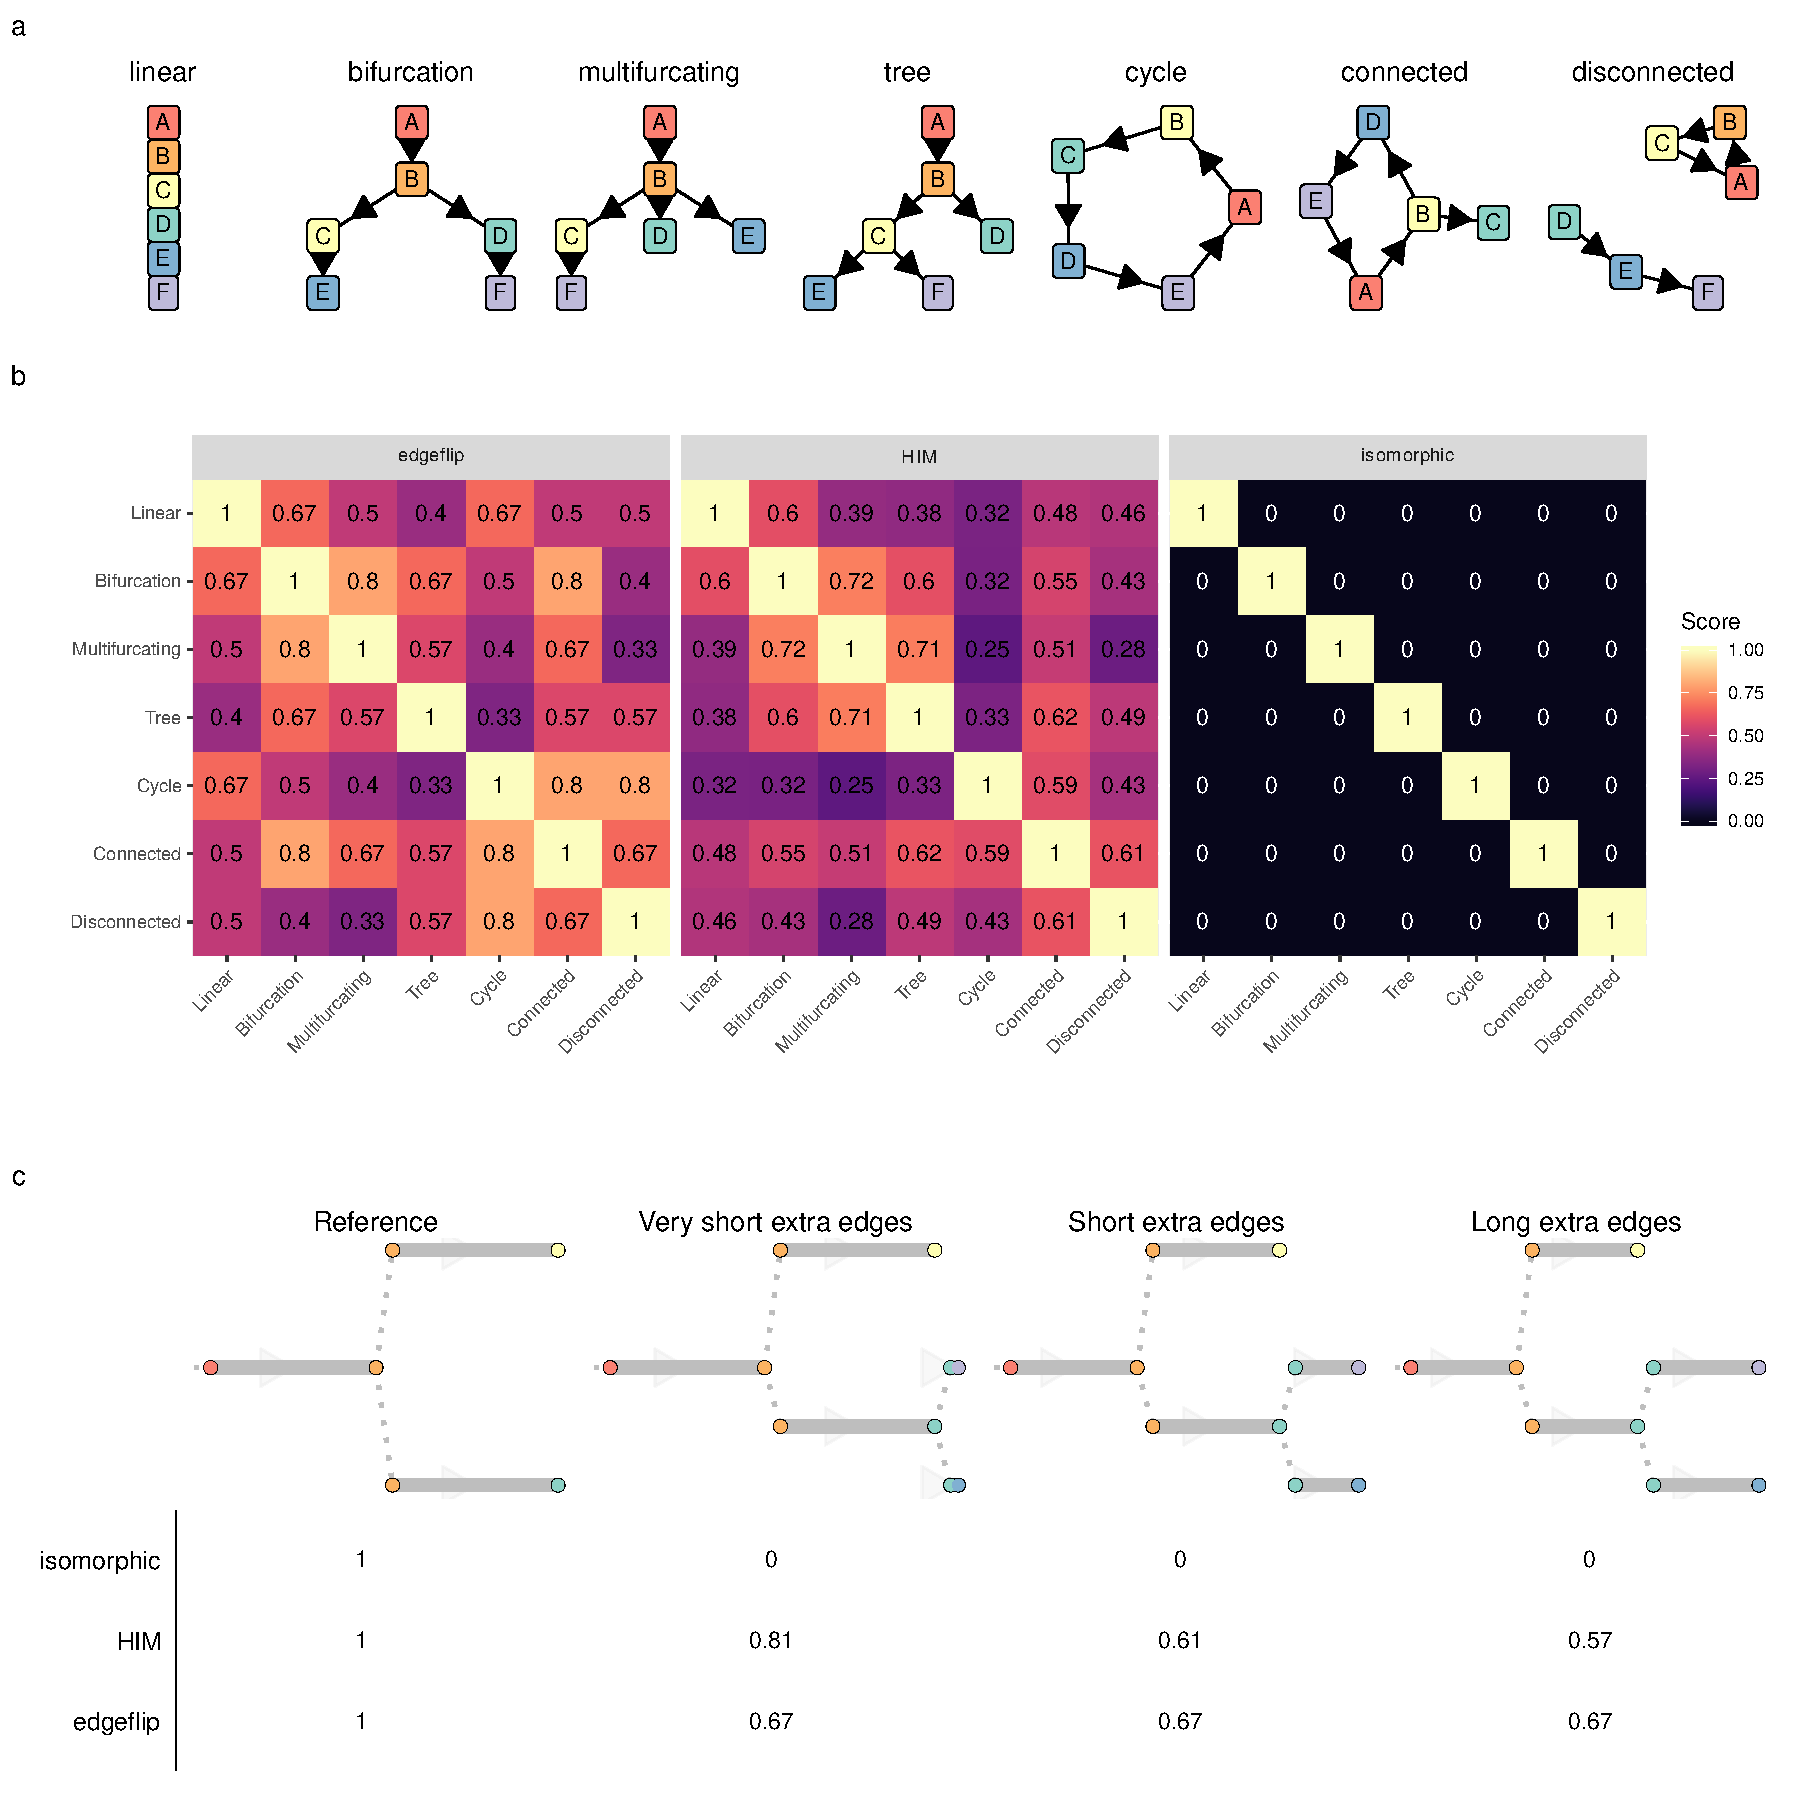
\includegraphics[width=\linewidth]{fig/snote1fig_2.pdf}
	\caption{
		\textbf{Showcase of three metrics to evaluate topologies: \textit{isomorphic}, \textit{edgeflip} and \textit{HIM}}
		\textbf{(a)} The used topologies. \textbf{(b)} The scores when comparing each pair of trajectory types. (c) Four datasets in which aan extra edge is added and made progressively longer. This shows how the HIM can take into account edge lengths.
	}
	\label{fig:snote1fig_2}
\end{figure}

To summarise, the different topology based scores are useful for different scenarios:

\begin{itemize}
	\item If the two trajectories should only be compared when the topology is exactly the same, the \textit{isomorphic} should be used.
	\item If it is important that the topologies are similar, but not necessarily isomorphic, the \textit{edgeflip} is most appropriate.
	\item If the topologies should be similar, but shorter edges should not be punished as hard as longer edges, the \textit{HIM} is most appropriate.
\end{itemize}

\subsubsection{$\textit{F1}_{\textit{branches}}$ and $\textit{F1}_{\textit{milestones}}$: Comparing how well the cells are clustered in the trajectory}

Perhaps one of the simplest ways to calculate the similarity between the cellular positions of two topologies is by mapping each cell to its closest milestone \textit{or} branch \ref{fig:snote1fig_3}. These clusters of cells can then be compared using one of the many external cluster evaluation measures \cite{saelens_comprehensiveevaluationmodule_2018}. When selecting a cluster evaluation metric, we had two main conditions:

- Because we allow methods to filter cells in the trajectory, the metric should be able to handle "non-exhaustive assignment", where some cells are not assigned to any cluster.
- The metric should give each cluster equal weight, so that rare cell stages are equally important as large stages.

The $\textit{F1}$ score between the $\textit{Recovery}$ and $\textit{Relevance}$ is a metric which conforms to both these conditions. This metric will map two clustersets by using their shared members based on the $\textit{Jaccard}$ similarity. It then calculates the $\textit{Recovery}$ as the average maximal $\textit{Jaccard}$ for every cluster in the first set of clusters (in our case the reference trajectory). Conversely, the $\textit{Relevance}$ is calculated based on the average maximal similarity in the second set of clusters (in our case the prediction). Both the $\textit{Recovery}$ and $\textit{Relevance}$ are then given equal weight in a harmonic mean ($\textit{F1}$). Formally, if $C$ and $C'$ are two cell clusters:

\begin{align*}
\textit{Jaccard}(c, c') &= \frac{|c \cap c'|}{|c \cup c'|} \\
\textit{Recovery} &= \frac{1}{|C|} \sum_{c \in C}{\max_{c' \in C'}{\textit{Jaccard(c, c')}}} \\
\textit{Relevance} &= \frac{1}{|C'|} \sum_{c' \in C'}{\max_{c \in C}{\textit{Jaccard(c, c')}}} \\
\textit{F1} &= \frac{2}{\frac{1}{\textit{Recovery}} + \frac{1}{\textit{Relevance}}}
\end{align*}

\begin{figure}[tbh!]
	\centering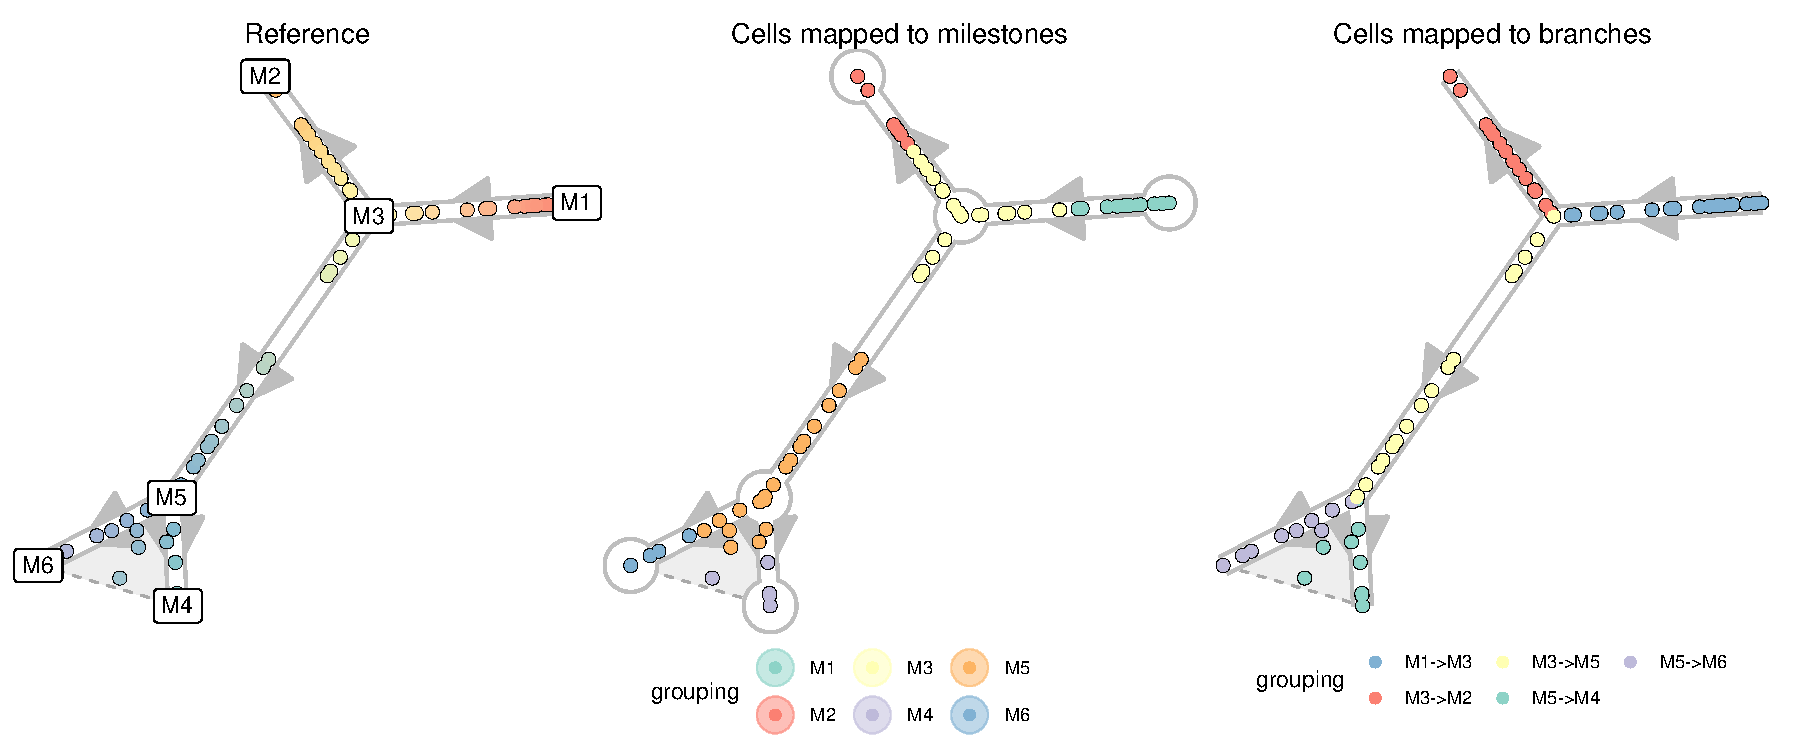
\includegraphics[width=\linewidth]{fig/snote1fig_3.pdf}
	\caption{
		\textbf{Mapping cells to their closest milestone or branch for the calculation of the {$\textit{F1}_{\textit{milestones}}$} and {$\textit{F1}_{\textit{branches}}$} .}
		To calculate the {$\textit{F1}_{\textit{milestones}}$}, cells are mapped towards the nearest milestone, i.e. the milestone with the highest milestone percentage. For the {$\textit{F1}_{\textit{branches}}$}, the cells are mapped to the closest edge.
	}
	\label{fig:snote1fig_3}
\end{figure}

\subsubsection{$\textit{cor}_{\textit{dist}}$: Correlation between geodesic distances}

When the position of a cell is the same in both the reference and the prediction, its \textit{relative} distances to all other cells in the trajectory should also be the same. This observation is the basis for the $\textit{cor}_{\textit{dist}}$ metric.

\begin{figure}[tbh!]
	\centering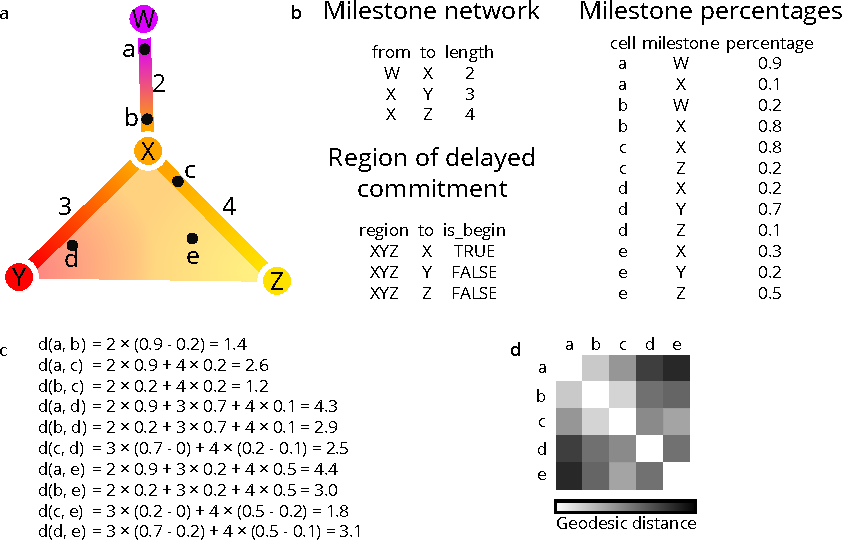
\includegraphics[width=\linewidth]{fig/snote1fig_4.pdf}
	\caption{
		\textbf{The calculation of geodesic distances on a small example trajectory.}
		\textbf{a)} A toy example containing four milestones (W to Z) and five cells (a to e). \textbf{b)} The corresponding milestone network, milestone percentages and regions of delayed commitment, when the toy trajectory is converted to the common trajectory model. \textbf{c)} The calculations made for calculating the pairwise geodesic distances. \textbf{d)} A heatmap representation of the pairwise geodesic distances.
	}
	\label{fig:snote1fig_4}
\end{figure}

The geodesic distance is the distance a cell has to go through the trajectory space to get from one position to another. The way this distance is calculated depends on how two cells are positioned, showcased by an example in Figure \ref{fig:snote1fig_4}:

\begin{itemize}
	\item \textbf{Both cells are on the same edge in the milestone network.} In this case, the geodesic distance is defined as the product of the difference in milestone percentages and the length of their shared edge. For cells $a$ and $b$ in the example, $d(a, b)$ is equal to $1 \times (0.9 - 0.2) = 0.7$.
	\item \textbf{Cells reside on different edges in the milestone network.} First, the distance of the cell to all its nearby milestones is calculated, based on its percentage within the edge and the length of the edge. These distances in combination with the milestone network are used to calculate the shortest path distance between the two cells. For cells $a$ and $c$ in the example, $d(a, X) = 1 \times 0.9$ and $d(c, X) = 3 \times 0.2$, and therefore $d(a, c) = 1 \times 0.9 + 3 \times 0.2$. 
\end{itemize}

The geodesic distance can be easily extended towards cells within regions of delayed commitment. When both cells are part of the same region of delayed commitment, the geodesic distance was defined as the manhattan distances between the milestone percentages weighted by the lengths from the milestone network. For cells $d$ and $e$ in the example, $d(d, e)$ is equal to $0 \times (0.3 - 0.2) + 2 \times (0.7 - 0.2) + 3 \times(0.4 - 0.1) = 1.9$. The distance between two cells where only one is part of a region of delayed commitment is calculated similarly to the previous paragraph, by first calculating the distance between the cells and their neighbouring milestones first, then calculating the shortest path distances between the two.

Calculating the pairwise distances between cells scales quadratically with the number of cells, and would therefore not be scaleable for large datasets. For this reason, a set of waypoint cells are defined \textit{a priori}, and only the distances between the waypoint cells and all other cells is calculated, in order to calculate the correlation of geodesic distances of two trajectories (Figure \ref{fig:snote1fig_5}a). These cell waypoints are determined by viewing each milestone, edge and region of delayed commitment as a collection of cells. We do stratified sampling from each collection of cells by weighing them by the total number of cells within that collection. For calculating the $\textit{cor}_{\textit{dist}}$ between two trajectories, the distances between all cells and the union of both waypoint sets is computed.

To select the number of cell waypoints, we need to find a trade-off between the accuracy versus the time to calculate $\textit{cor}_{\textit{dist}}$. To select an optimal number of cell waypoints, we used the synthetic dataset with the most complex topology, and determined the $\textit{cor}_{\textit{dist}}$ at different levels of both cell shuffling and number of cell waypoints (Figure \ref{fig:snote1fig_5}a). We found that using cell waypoints does not induce a systematic bias in the $\textit{cor}_{\textit{dist}}$, and that its variability was relatively minimal when compared to the variability between different levels of cell shuffling when using 100 or more cell waypoints.

\begin{figure}[tbh!]
	\centering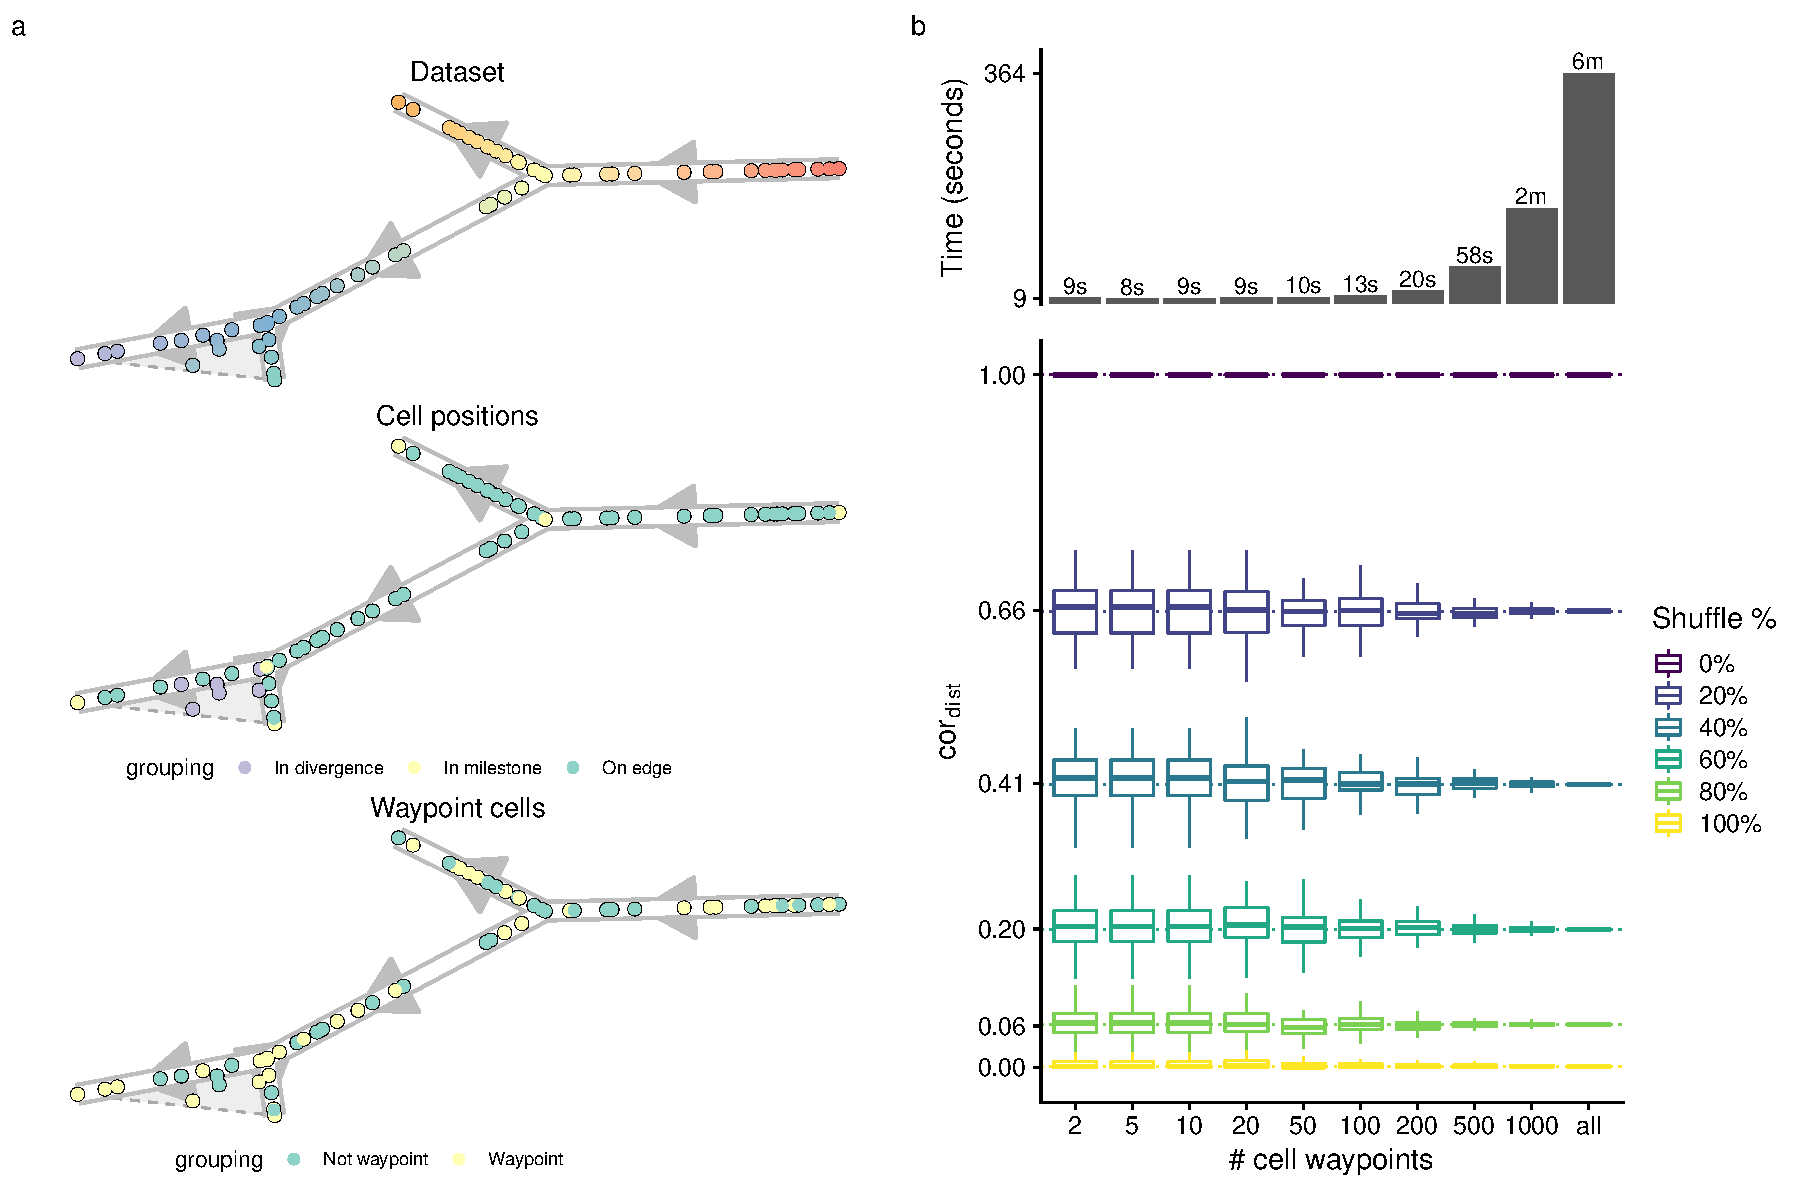
\includegraphics[width=\linewidth]{fig/snote1fig_5.pdf}
	\caption{
		\textbf{Determination of cell waypoints} \textbf{a)} Illustration of the stratified cell sampling using an example dataset (top). Each milestone, edge between two milestones and region of delayed commitment is seen as a collection of cells (middle), and the number of waypoints (100 in this case) are divided over each of these collection of cells (bottom). \textbf{b)} Accuracy versus time to calculate $\textit{cor}_{\textit{dist}}$. Shown are distributions over 100 random waypoint samples. The upper whisker of the boxplot extends from the hinge (75$\%$ percentile) to the largest value, no further than 1.5$\times$ the IQR of the hinge. The lower whisker extends from the hinge (25$\%$ percentile) to the smallest value, at most 1.5$\times$ the IQR of the hinge.
	}
	\label{fig:snote1fig_5}
\end{figure}

Although the $\textit{cor}_{\textit{dist}}$'s main characteristic is that it looks at the positions of the cells, other features of the trajectory are also (partly) captured. To illustrate this, we used the geodesic distances themselves as input for dimensionality reduction (Figure \ref{fig:snote1fig_6}) with varying topologies. This reduced space captures the original trajectory structure quite well, including the overall topology and branch lengths.

\begin{figure}[tbh!]
	\centering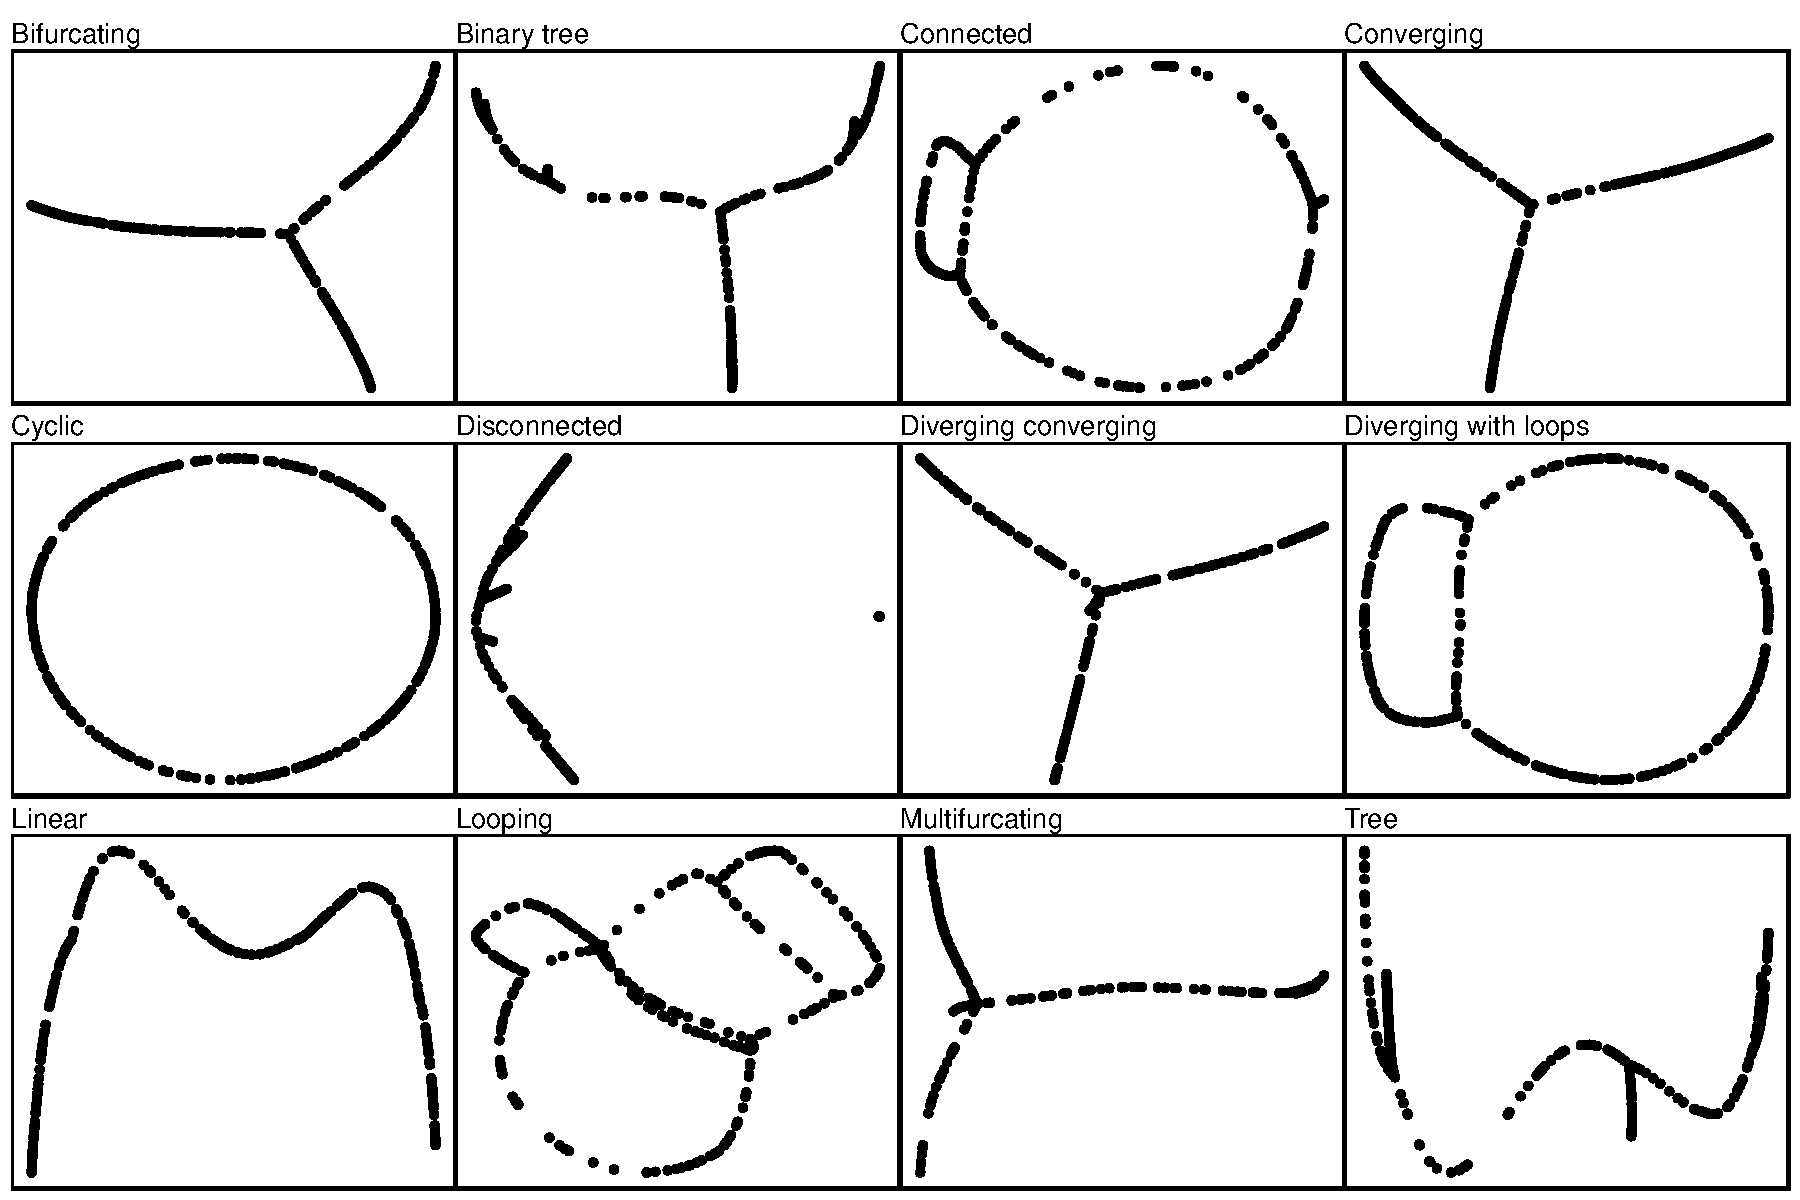
\includegraphics[width=\linewidth]{fig/snote1fig_6.pdf}
	\caption{
		\textbf{Determination of cell waypoints.} 
		We generated different toy trajectory datasets with varying topologies and calculated the geodesic distances between all cells within the trajectory. We then used these distances as input for classical multidimensional scaling. This shows that the geodesic distances do not only contain information regarding the cell's positions, but also information on the lengths and wiring of the topology.
	}
	\label{fig:snote1fig_6}
\end{figure}

\subsubsection{$\textit{NMSE}_{\textit{rf}}$ and $\textit{NMSE}_{\textit{lm}}$: Using the positions of the cells within one trajectory to predict the cellular positions in the other trajectory}

An alternative approach to detect whether the positions of cells are similar between two trajectories, is to use the positions of one trajectory to predict the positions within the other trajectory. If the cells are at similar positions in the trajectory (relative to its nearby cells), the prediction error should be low.

Specifically, we implemented two metrics which predict the milestone percentages from the reference by using the predicted milestone percentages as features (Figure \ref{fig:snote1fig_7}). We did this with two regression methods, linear regression ($\textit{lm}$, using the R lm function) and Random Forest ($\textit{rf}$, implemented in the \textit{ranger} package  \cite{wright_rangerfastimplementation_2017}). In both cases, the accuracy of the prediction was measured using the Mean Squared error ($\mathit{MSE}$), in the case of Random forest we used the out-of-bag mean-squared error. Next, we calculated $\mathit{MSE}_{worst}$ equal to the $\mathit{MSE}$ when predicting all milestone percentages as the average. We used this to calculate the normalised mean squared error as $\mathit{NMSE} = 1 - \frac{\mathit{MSE}}{\mathit{MSE}_{worst}}$. We created a regression model for every milestone in the gold standard, and averaged the $\mathit{NMSE}$ values to finally obtain the $\textit{NMSE}_{\textit{rf}}$ and $\textit{NMSE}_{\textit{lm}}$ scores.

\begin{figure}[tbh!]
	\centering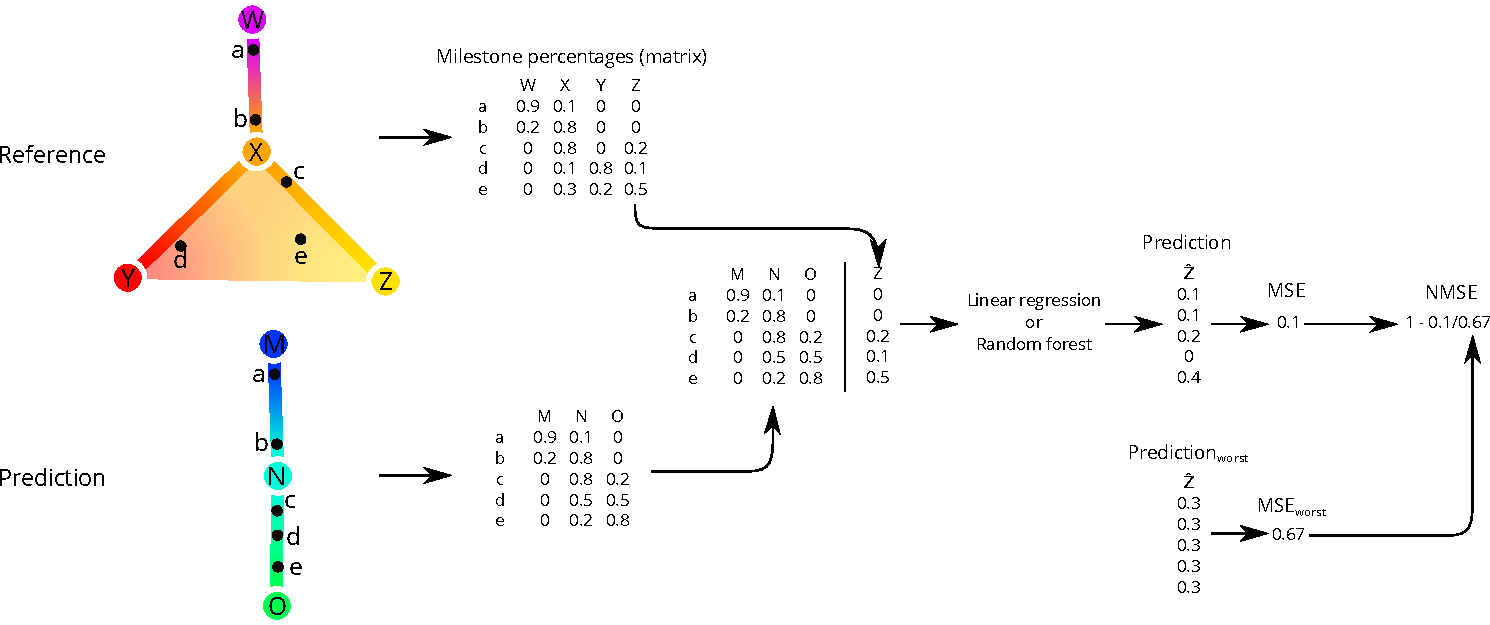
\includegraphics[width=\linewidth]{fig/snote1fig_7.pdf}
	\caption{
		\textbf{The calculation of $\textit{NMSE}_{\textit{lm}}$ distances on a small example trajectory.} 
		The milestone percentages of the reference are predicted based on the milestone percentages of the prediction, using regression models such as linear regression or random forests. The predicted trajectory is then scored by comparing the mean-squared error (MSE) of this regression model with the baseline MSE where the prediction is the average milestone percentage.
	}
	\label{fig:snote1fig_7}
\end{figure}

\subsubsection{$\textit{cor}_{\textit{features}}$ and $\textit{wcor}_{\textit{features}}$: The accuracy of dynamical differentially expressed features/genes.}

Although most metrics described above already assess some aspects directly relevant to the user, such as whether the method is good at finding the right topology, these metrics do not assess the quality of downstream analyses and hypotheses which can be generated from these models. 

Perhaps the main advantage of studying cellular dynamic processes using single-cell -omics data is that the dynamics of gene expression can be studied for the whole transcriptome. This can be used to construct other models such as dynamic regulatory networks and gene expression modules. Such analyses rely on a "good-enough" cellular ordering, so that it can be used to identify dynamical differentially expressed genes.

To calculate the $\textit{cor}_{\textit{features}}$ we used Random forest regression to rank all the features according to their importance in predicting the positions of cells in the trajectory. More specifically, we first calculated the geodesic distances for each cell to all milestones in the trajectory. Next, we trained a Random Forest regression model (implemented in the R \textit{ranger} package \cite{wright_rangerfastimplementation_2017}, \url{https://github.com/imbs-hl/ranger}) to predict these distances for each milestone, based on the expression of genes within each cell. We then extracted feature importances using the Mean Decrease in Impurity (importance = 'impurity' parameter of the ranger function), as illustrated in Figure \ref{fig:snote1fig_8}. The overall importance of a feature (gene) was then equal to the mean importance over all milestones. Finally, we compared the two rankings by calculating the Pearson correlation, with values between -1 and 0 clipped to 0.

\begin{figure}[tbh!]
	\centering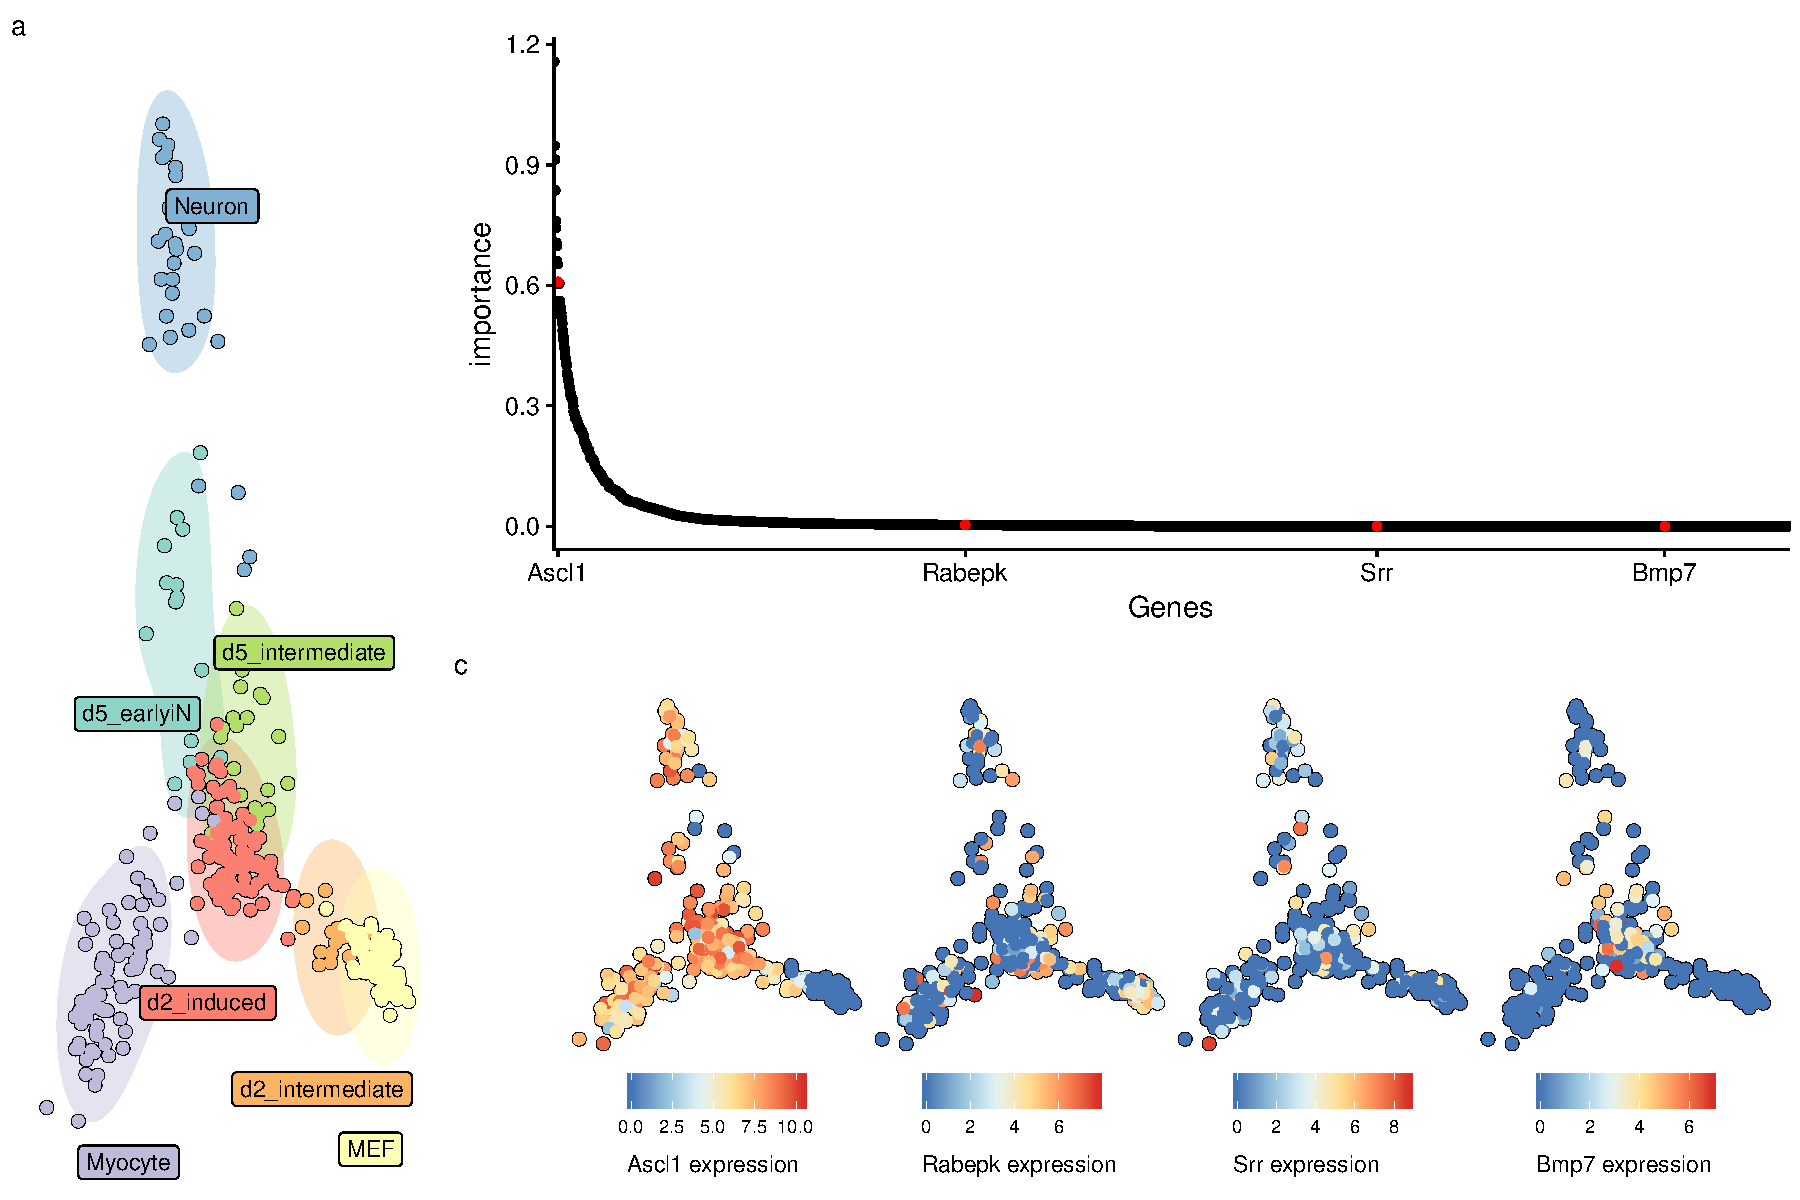
\includegraphics[width=\linewidth]{fig/snote1fig_8.pdf}
	\caption{
		\textbf{An illustration of ranking features based on their importance in a trajectory.} 
		(a) A MDS dimensionality reduction of a real dataset in which mouse embryonic fibroblasts (MEF) differentiate into Neurons and Myocytes. (b) The ranking of feature importances from high to low. The majority of features have a very low importance. (c) Some examples, which were also highlighted in b. Higher features in the ranking are clearly specific to certain parts of the trajectory, while features lower on the ranking have a more dispersed expression pattern.
	}
	\label{fig:snote1fig_8}
\end{figure}

Random forest regression has two main hyperparameters. The number of trees to be fitted (num\_tree parameter) was fixed to 10000 to provide accurate and stable estimates of the feature importance (Figure \ref{fig:snote1fig_9}. The number of features on which can be split (mtry parameter) was set to 1$\%$ of all available features (instead of the default square-root of the number of features), as to make sure that predictive but highly correlated features, omnipresent in transcriptomics data, are not suppressed in the ranking.

\begin{figure}[tbh!]
	\centering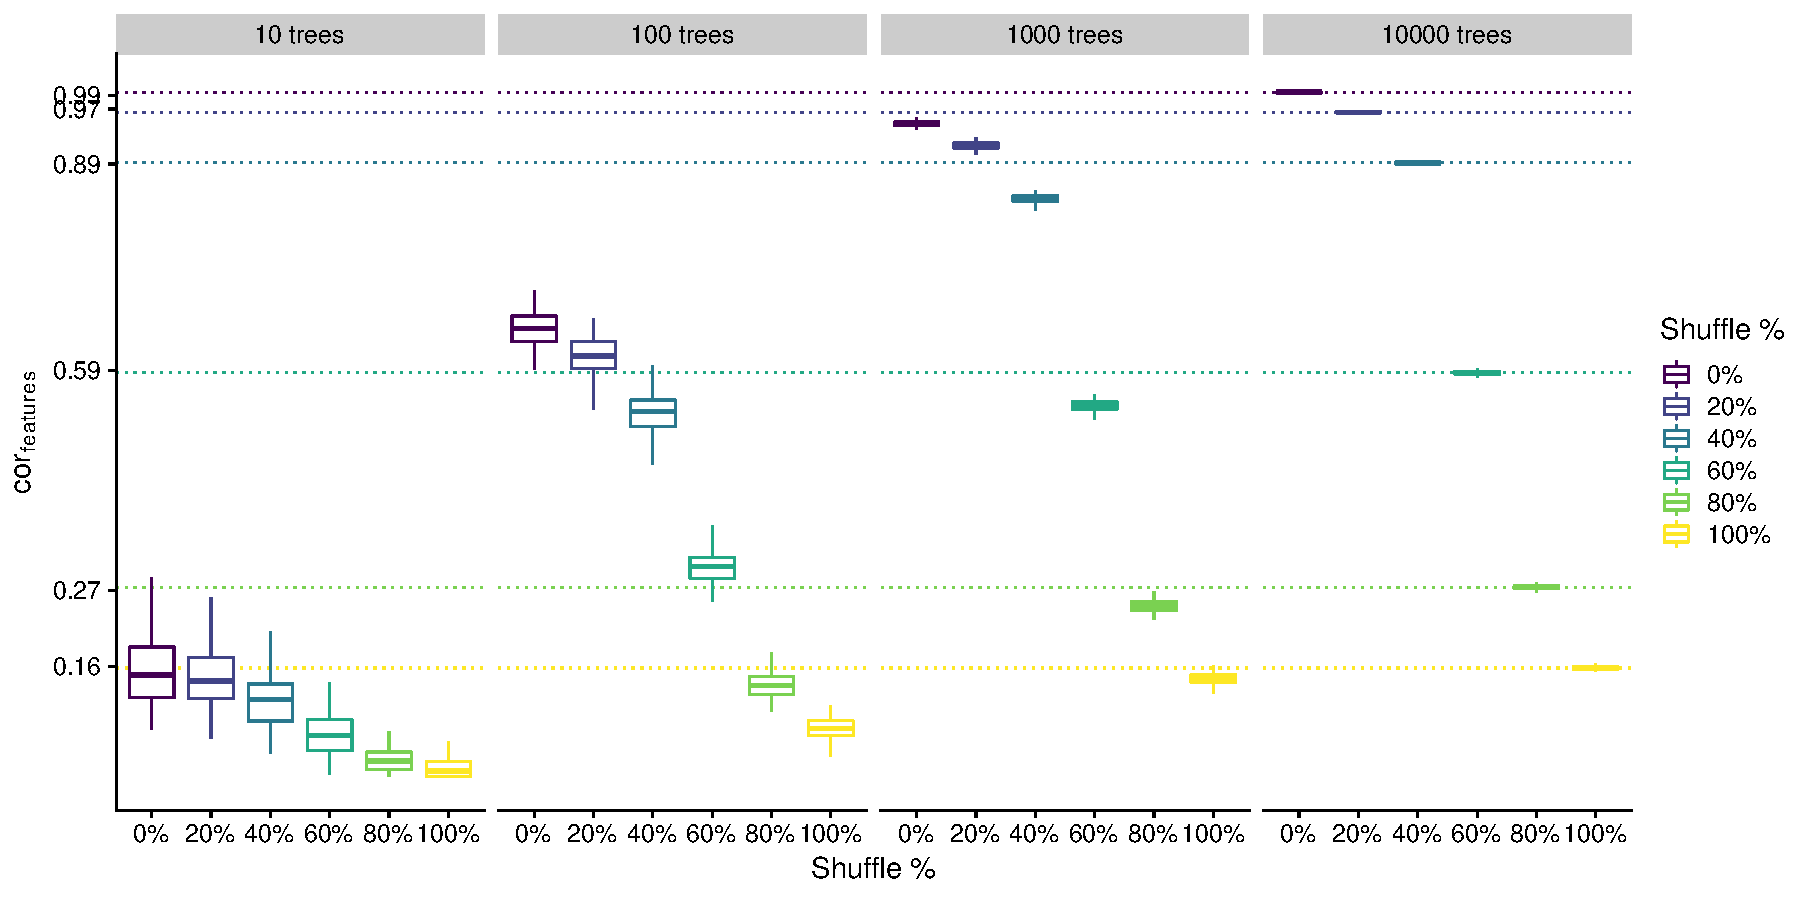
\includegraphics[width=\linewidth]{fig/snote1fig_9.pdf}
	\caption{
		\textbf{Effect of the number of trees parameter on the accuracy and variability of the $\textit{cor}_{\textit{features}}$.} 
		We used the dataset from Figure \ref{fig:snote1fig_8} and calculated the $\textit{cor}_{\textit{features}}$ after shuffling a percentage of cells.
	}
	\label{fig:snote1fig_9}
\end{figure}

For most datasets, only a limited number of features will be differentially expressed in the trajectory. For example, in the dataset used in Figure \ref{fig:snote1fig_9} only the top 10$\%$-20$\%$ show a clear pattern of differential expression. The correlation will weight each of these features equally, and will therefore give more weight to the bottom, irrelevant features. To prioritise the top differentially expressed features, we also implemented the $\textit{wcor}_{\textit{features}}$, which will weight the correlation using the feature importance scores in the reference so that the top features have relatively more impact on the score (Figure \ref{fig:snote1fig_10}).

\begin{figure}[tbh!]
	\centering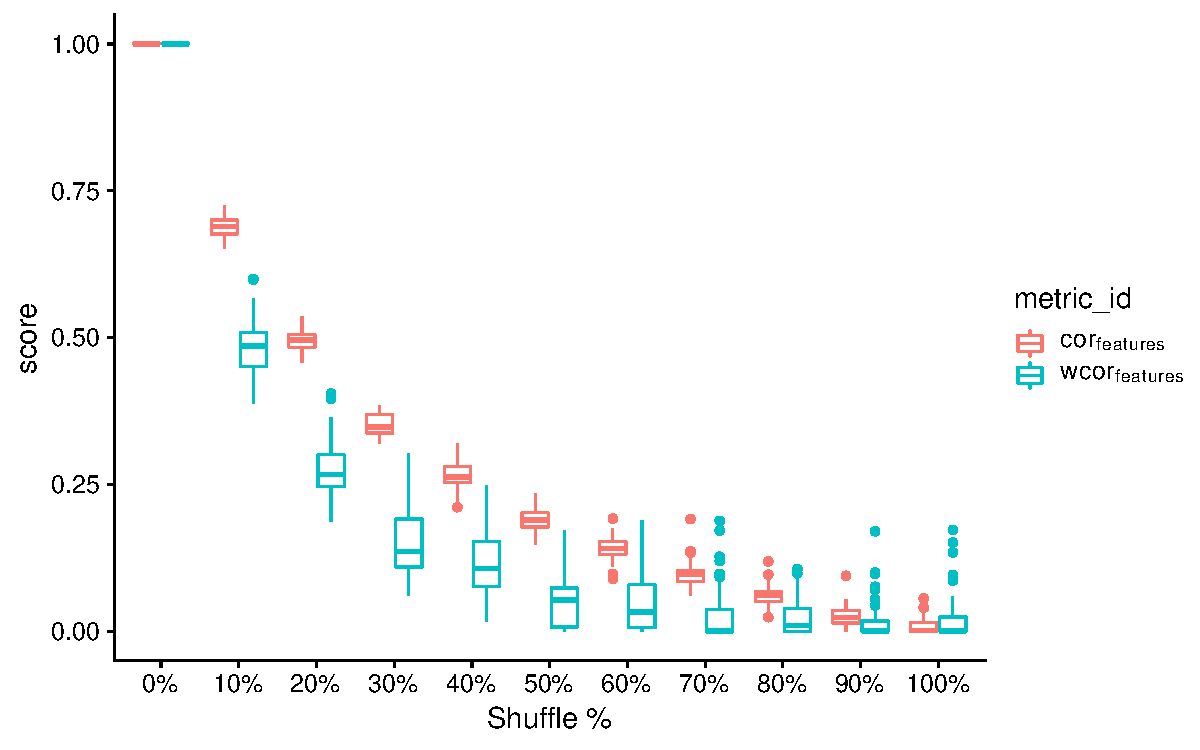
\includegraphics[width=\linewidth]{fig/snote1fig_10.pdf}
	\caption{
		\textbf{Effect of weighting the features based on their feature importance in the reference.} 
		We used the same dataset as in Figure \ref{fig:snote1fig_8}, and calculated the $\textit{cor}_{\textit{features}}$ after shuffling a percentage of cells.
	}
	\label{fig:snote1fig_10}
\end{figure}

% TODO: check floatbarrier?
%\FloatBarrier

\subsection{Metric conformity}

Although most metrics described in the previous section make sense intuitively, this does not necessarily mean that these metrics are robust and will generate reasonable results when used for benchmarking. This is because different methods and datasets will all lead to a varied set of trajectory models:

\begin{itemize}
	\item Real datasets have all cells grouped onto milestones
	\item Some methods place all cells in a region of delayed commitment, others never generate a region of delayed commitment
	\item Some methods always return a linear trajectory, even if a bifurcation is present in the data
	\item Some methods filter cells
\end{itemize}

A good metric, especially a good overall metric, should work in all these circumstances. To test this, we designed a set of rules to which a good metric should conform, and assessed empirically whether a metric conforms to these rules.

We generated a panel of toy datasets (using our \textit{dyntoy} package, \url{https://github.com/dynverse/dyntoy}) with all possible combinations of:

\begin{itemize}
	\item \# cells: 10, 20, 50, 100, 200, 500
	\item \# features: 200
	\item topologies: linear, bifurcation, multifurcating, tree, cycle, connected graph and disconnected graph
	\item Whether cells are placed on the milestones (as in real data) or on the edges/regions of delayed commitment between the milestones (as in synthetic data)
\end{itemize}

We then perturbed the trajectories in these datasets in certain ways, and tested whether the scores follow an expected pattern. An overview of the conformity of every metric is first given in Table \ref{tab:conformity_overview}. The individual rules and metric behaviour are discussed in the Supplementary Material that can be found at \url{https://www.nature.com/articles/s41587-019-0071-9\#Sec34}.

\begin{table}
	\caption{Overview of whether a particular metric conforms to a particular rule} \label{tab:conformity_overview}
	
	\centering\begingroup\fontsize{7}{9}\selectfont
	
	\begin{tabular}{>{\raggedright\arraybackslash}p{15em}>{\raggedright\arraybackslash}p{1em}>{\raggedright\arraybackslash}p{1em}>{\raggedright\arraybackslash}p{1em}>{\raggedright\arraybackslash}p{1em}>{\raggedright\arraybackslash}p{1em}>{\raggedright\arraybackslash}p{1em}>{\raggedright\arraybackslash}p{1em}>{\raggedright\arraybackslash}p{1em}>{\raggedright\arraybackslash}p{1em}>{\raggedright\arraybackslash}p{1em}>{\raggedright\arraybackslash}p{1em}}
		\toprule
		\rotatebox{0}{name} & \rotatebox{90}{$\textit{cor}_{\textit{dist}}$} & \rotatebox{90}{$\textit{NMSE}_{\textit{rf}}$} & \rotatebox{90}{$\textit{NMSE}_{\textit{lm}}$} & \rotatebox{90}{$\textit{edgeflip}$} & \rotatebox{90}{$\textit{HIM}$} & \rotatebox{90}{isomorphic} & \rotatebox{90}{$\textit{cor}_{\textit{features}}$} & \rotatebox{90}{$\textit{wcor}_{\textit{features}}$} & \rotatebox{90}{$\textit{F1}_{\textit{branches}}$} & \rotatebox{90}{$\textit{F1}_{\textit{milestones}}$} & \rotatebox{90}{$\textit{mean}_{\textit{geometric}}$}\\
		\midrule
		Same score on identity & \multicolumn{1}{c}{\cellcolor[HTML]{B2DF8A}{\cmark}} & \multicolumn{1}{c}{\cellcolor[HTML]{FB9A99}{\xmark}} & \multicolumn{1}{c}{\cellcolor[HTML]{B2DF8A}{\cmark}} & \multicolumn{1}{c}{\cellcolor[HTML]{B2DF8A}{\cmark}} & \multicolumn{1}{c}{\cellcolor[HTML]{B2DF8A}{\cmark}} & \multicolumn{1}{c}{\cellcolor[HTML]{B2DF8A}{\cmark}} & \multicolumn{1}{c}{\cellcolor[HTML]{B2DF8A}{\cmark}} & \multicolumn{1}{c}{\cellcolor[HTML]{FB9A99}{\xmark}} & \multicolumn{1}{c}{\cellcolor[HTML]{B2DF8A}{\cmark}} & \multicolumn{1}{c}{\cellcolor[HTML]{B2DF8A}{\cmark}} & \multicolumn{1}{c}{\cellcolor[HTML]{B2DF8A}{\cmark}}\\
		Local cell shuffling & \multicolumn{1}{c}{\cellcolor[HTML]{B2DF8A}{\cmark}} & \multicolumn{1}{c}{\cellcolor[HTML]{B2DF8A}{\cmark}} & \multicolumn{1}{c}{\cellcolor[HTML]{B2DF8A}{\cmark}} & \multicolumn{1}{c}{\cellcolor[HTML]{FB9A99}{\xmark}} & \multicolumn{1}{c}{\cellcolor[HTML]{FB9A99}{\xmark}} & \multicolumn{1}{c}{\cellcolor[HTML]{FB9A99}{\xmark}} & \multicolumn{1}{c}{\cellcolor[HTML]{B2DF8A}{\cmark}} & \multicolumn{1}{c}{\cellcolor[HTML]{B2DF8A}{\cmark}} & \multicolumn{1}{c}{\cellcolor[HTML]{FB9A99}{\xmark}} & \multicolumn{1}{c}{\cellcolor[HTML]{B2DF8A}{\cmark}} & \multicolumn{1}{c}{\cellcolor[HTML]{B2DF8A}{\cmark}}\\
		Edge shuffling & \multicolumn{1}{c}{\cellcolor[HTML]{B2DF8A}{\cmark}} & \multicolumn{1}{c}{\cellcolor[HTML]{B2DF8A}{\cmark}} & \multicolumn{1}{c}{\cellcolor[HTML]{B2DF8A}{\cmark}} & \multicolumn{1}{c}{\cellcolor[HTML]{FB9A99}{\xmark}} & \multicolumn{1}{c}{\cellcolor[HTML]{FB9A99}{\xmark}} & \multicolumn{1}{c}{\cellcolor[HTML]{FB9A99}{\xmark}} & \multicolumn{1}{c}{\cellcolor[HTML]{B2DF8A}{\cmark}} & \multicolumn{1}{c}{\cellcolor[HTML]{B2DF8A}{\cmark}} & \multicolumn{1}{c}{\cellcolor[HTML]{B2DF8A}{\cmark}} & \multicolumn{1}{c}{\cellcolor[HTML]{B2DF8A}{\cmark}} & \multicolumn{1}{c}{\cellcolor[HTML]{B2DF8A}{\cmark}}\\
		Local and global cell shuffling & \multicolumn{1}{c}{\cellcolor[HTML]{B2DF8A}{\cmark}} & \multicolumn{1}{c}{\cellcolor[HTML]{B2DF8A}{\cmark}} & \multicolumn{1}{c}{\cellcolor[HTML]{B2DF8A}{\cmark}} & \multicolumn{1}{c}{\cellcolor[HTML]{FB9A99}{\xmark}} & \multicolumn{1}{c}{\cellcolor[HTML]{FB9A99}{\xmark}} & \multicolumn{1}{c}{\cellcolor[HTML]{FB9A99}{\xmark}} & \multicolumn{1}{c}{\cellcolor[HTML]{B2DF8A}{\cmark}} & \multicolumn{1}{c}{\cellcolor[HTML]{B2DF8A}{\cmark}} & \multicolumn{1}{c}{\cellcolor[HTML]{B2DF8A}{\cmark}} & \multicolumn{1}{c}{\cellcolor[HTML]{B2DF8A}{\cmark}} & \multicolumn{1}{c}{\cellcolor[HTML]{B2DF8A}{\cmark}}\\
		Changing positions locally and/or globally & \multicolumn{1}{c}{\cellcolor[HTML]{B2DF8A}{\cmark}} & \multicolumn{1}{c}{\cellcolor[HTML]{B2DF8A}{\cmark}} & \multicolumn{1}{c}{\cellcolor[HTML]{B2DF8A}{\cmark}} & \multicolumn{1}{c}{\cellcolor[HTML]{FB9A99}{\xmark}} & \multicolumn{1}{c}{\cellcolor[HTML]{FB9A99}{\xmark}} & \multicolumn{1}{c}{\cellcolor[HTML]{FB9A99}{\xmark}} & \multicolumn{1}{c}{\cellcolor[HTML]{B2DF8A}{\cmark}} & \multicolumn{1}{c}{\cellcolor[HTML]{B2DF8A}{\cmark}} & \multicolumn{1}{c}{\cellcolor[HTML]{FB9A99}{\xmark}} & \multicolumn{1}{c}{\cellcolor[HTML]{FB9A99}{\xmark}} & \multicolumn{1}{c}{\cellcolor[HTML]{B2DF8A}{\cmark}}\\
		
		Cell filtering & \multicolumn{1}{c}{\cellcolor[HTML]{B2DF8A}{\cmark}} & \multicolumn{1}{c}{\cellcolor[HTML]{B2DF8A}{\cmark}} & \multicolumn{1}{c}{\cellcolor[HTML]{B2DF8A}{\cmark}} & \multicolumn{1}{c}{\cellcolor[HTML]{FB9A99}{\xmark}} & \multicolumn{1}{c}{\cellcolor[HTML]{FB9A99}{\xmark}} & \multicolumn{1}{c}{\cellcolor[HTML]{FB9A99}{\xmark}} & \multicolumn{1}{c}{\cellcolor[HTML]{B2DF8A}{\cmark}} & \multicolumn{1}{c}{\cellcolor[HTML]{B2DF8A}{\cmark}} & \multicolumn{1}{c}{\cellcolor[HTML]{B2DF8A}{\cmark}} & \multicolumn{1}{c}{\cellcolor[HTML]{B2DF8A}{\cmark}} & \multicolumn{1}{c}{\cellcolor[HTML]{B2DF8A}{\cmark}}\\
		Removing divergence regions & \multicolumn{1}{c}{\cellcolor[HTML]{B2DF8A}{\cmark}} & \multicolumn{1}{c}{\cellcolor[HTML]{B2DF8A}{\cmark}} & \multicolumn{1}{c}{\cellcolor[HTML]{B2DF8A}{\cmark}} & \multicolumn{1}{c}{\cellcolor[HTML]{FB9A99}{\xmark}} & \multicolumn{1}{c}{\cellcolor[HTML]{FB9A99}{\xmark}} & \multicolumn{1}{c}{\cellcolor[HTML]{FB9A99}{\xmark}} & \multicolumn{1}{c}{\cellcolor[HTML]{B2DF8A}{\cmark}} & \multicolumn{1}{c}{\cellcolor[HTML]{B2DF8A}{\cmark}} & \multicolumn{1}{c}{\cellcolor[HTML]{FB9A99}{\xmark}} & \multicolumn{1}{c}{\cellcolor[HTML]{B2DF8A}{\cmark}} & \multicolumn{1}{c}{\cellcolor[HTML]{B2DF8A}{\cmark}}\\
		Move cells to start milestone & \multicolumn{1}{c}{\cellcolor[HTML]{B2DF8A}{\cmark}} & \multicolumn{1}{c}{\cellcolor[HTML]{B2DF8A}{\cmark}} & \multicolumn{1}{c}{\cellcolor[HTML]{B2DF8A}{\cmark}} & \multicolumn{1}{c}{\cellcolor[HTML]{FB9A99}{\xmark}} & \multicolumn{1}{c}{\cellcolor[HTML]{FB9A99}{\xmark}} & \multicolumn{1}{c}{\cellcolor[HTML]{FB9A99}{\xmark}} & \multicolumn{1}{c}{\cellcolor[HTML]{B2DF8A}{\cmark}} & \multicolumn{1}{c}{\cellcolor[HTML]{B2DF8A}{\cmark}} & \multicolumn{1}{c}{\cellcolor[HTML]{FB9A99}{\xmark}} & \multicolumn{1}{c}{\cellcolor[HTML]{B2DF8A}{\cmark}} & \multicolumn{1}{c}{\cellcolor[HTML]{B2DF8A}{\cmark}}\\
		Move cells to closest milestone & \multicolumn{1}{c}{\cellcolor[HTML]{B2DF8A}{\cmark}} & \multicolumn{1}{c}{\cellcolor[HTML]{B2DF8A}{\cmark}} & \multicolumn{1}{c}{\cellcolor[HTML]{B2DF8A}{\cmark}} & \multicolumn{1}{c}{\cellcolor[HTML]{FB9A99}{\xmark}} & \multicolumn{1}{c}{\cellcolor[HTML]{FB9A99}{\xmark}} & \multicolumn{1}{c}{\cellcolor[HTML]{FB9A99}{\xmark}} & \multicolumn{1}{c}{\cellcolor[HTML]{B2DF8A}{\cmark}} & \multicolumn{1}{c}{\cellcolor[HTML]{B2DF8A}{\cmark}} & \multicolumn{1}{c}{\cellcolor[HTML]{FB9A99}{\xmark}} & \multicolumn{1}{c}{\cellcolor[HTML]{B2DF8A}{\cmark}} & \multicolumn{1}{c}{\cellcolor[HTML]{B2DF8A}{\cmark}}\\
		Length shuffling & \multicolumn{1}{c}{\cellcolor[HTML]{B2DF8A}{\cmark}} & \multicolumn{1}{c}{\cellcolor[HTML]{FB9A99}{\xmark}} & \multicolumn{1}{c}{\cellcolor[HTML]{B2DF8A}{\cmark}} & \multicolumn{1}{c}{\cellcolor[HTML]{FB9A99}{\xmark}} & \multicolumn{1}{c}{\cellcolor[HTML]{B2DF8A}{\cmark}} & \multicolumn{1}{c}{\cellcolor[HTML]{FB9A99}{\xmark}} & \multicolumn{1}{c}{\cellcolor[HTML]{FB9A99}{\xmark}} & \multicolumn{1}{c}{\cellcolor[HTML]{FB9A99}{\xmark}} & \multicolumn{1}{c}{\cellcolor[HTML]{FB9A99}{\xmark}} & \multicolumn{1}{c}{\cellcolor[HTML]{B2DF8A}{\cmark}} & \multicolumn{1}{c}{\cellcolor[HTML]{B2DF8A}{\cmark}}\\
		
		Cells into small subedges & \multicolumn{1}{c}{\cellcolor[HTML]{FB9A99}{\xmark}} & \multicolumn{1}{c}{\cellcolor[HTML]{B2DF8A}{\cmark}} & \multicolumn{1}{c}{\cellcolor[HTML]{FB9A99}{\xmark}} & \multicolumn{1}{c}{\cellcolor[HTML]{B2DF8A}{\cmark}} & \multicolumn{1}{c}{\cellcolor[HTML]{B2DF8A}{\cmark}} & \multicolumn{1}{c}{\cellcolor[HTML]{B2DF8A}{\cmark}} & \multicolumn{1}{c}{\cellcolor[HTML]{B2DF8A}{\cmark}} & \multicolumn{1}{c}{\cellcolor[HTML]{FB9A99}{\xmark}} & \multicolumn{1}{c}{\cellcolor[HTML]{B2DF8A}{\cmark}} & \multicolumn{1}{c}{\cellcolor[HTML]{B2DF8A}{\cmark}} & \multicolumn{1}{c}{\cellcolor[HTML]{B2DF8A}{\cmark}}\\
		New leaf edges & \multicolumn{1}{c}{\cellcolor[HTML]{B2DF8A}{\cmark}} & \multicolumn{1}{c}{\cellcolor[HTML]{B2DF8A}{\cmark}} & \multicolumn{1}{c}{\cellcolor[HTML]{FB9A99}{\xmark}} & \multicolumn{1}{c}{\cellcolor[HTML]{B2DF8A}{\cmark}} & \multicolumn{1}{c}{\cellcolor[HTML]{B2DF8A}{\cmark}} & \multicolumn{1}{c}{\cellcolor[HTML]{B2DF8A}{\cmark}} & \multicolumn{1}{c}{\cellcolor[HTML]{FB9A99}{\xmark}} & \multicolumn{1}{c}{\cellcolor[HTML]{FB9A99}{\xmark}} & \multicolumn{1}{c}{\cellcolor[HTML]{B2DF8A}{\cmark}} & \multicolumn{1}{c}{\cellcolor[HTML]{B2DF8A}{\cmark}} & \multicolumn{1}{c}{\cellcolor[HTML]{B2DF8A}{\cmark}}\\
		New connecting edges & \multicolumn{1}{c}{\cellcolor[HTML]{B2DF8A}{\cmark}} & \multicolumn{1}{c}{\cellcolor[HTML]{B2DF8A}{\cmark}} & \multicolumn{1}{c}{\cellcolor[HTML]{FB9A99}{\xmark}} & \multicolumn{1}{c}{\cellcolor[HTML]{B2DF8A}{\cmark}} & \multicolumn{1}{c}{\cellcolor[HTML]{B2DF8A}{\cmark}} & \multicolumn{1}{c}{\cellcolor[HTML]{B2DF8A}{\cmark}} & \multicolumn{1}{c}{\cellcolor[HTML]{B2DF8A}{\cmark}} & \multicolumn{1}{c}{\cellcolor[HTML]{B2DF8A}{\cmark}} & \multicolumn{1}{c}{\cellcolor[HTML]{B2DF8A}{\cmark}} & \multicolumn{1}{c}{\cellcolor[HTML]{B2DF8A}{\cmark}} & \multicolumn{1}{c}{\cellcolor[HTML]{B2DF8A}{\cmark}}\\
		Changing topology and cell position & \multicolumn{1}{c}{\cellcolor[HTML]{FB9A99}{\xmark}} & \multicolumn{1}{c}{\cellcolor[HTML]{FB9A99}{\xmark}} & \multicolumn{1}{c}{\cellcolor[HTML]{FB9A99}{\xmark}} & \multicolumn{1}{c}{\cellcolor[HTML]{FB9A99}{\xmark}} & \multicolumn{1}{c}{\cellcolor[HTML]{FB9A99}{\xmark}} & \multicolumn{1}{c}{\cellcolor[HTML]{FB9A99}{\xmark}} & \multicolumn{1}{c}{\cellcolor[HTML]{FB9A99}{\xmark}} & \multicolumn{1}{c}{\cellcolor[HTML]{FB9A99}{\xmark}} & \multicolumn{1}{c}{\cellcolor[HTML]{FB9A99}{\xmark}} & \multicolumn{1}{c}{\cellcolor[HTML]{FB9A99}{\xmark}} & \multicolumn{1}{c}{\cellcolor[HTML]{B2DF8A}{\cmark}}\\
		Bifurcation merging & \multicolumn{1}{c}{\cellcolor[HTML]{B2DF8A}{\cmark}} & \multicolumn{1}{c}{\cellcolor[HTML]{FB9A99}{\xmark}} & \multicolumn{1}{c}{\cellcolor[HTML]{B2DF8A}{\cmark}} & \multicolumn{1}{c}{\cellcolor[HTML]{B2DF8A}{\cmark}} & \multicolumn{1}{c}{\cellcolor[HTML]{B2DF8A}{\cmark}} & \multicolumn{1}{c}{\cellcolor[HTML]{B2DF8A}{\cmark}} & \multicolumn{1}{c}{\cellcolor[HTML]{B2DF8A}{\cmark}} & \multicolumn{1}{c}{\cellcolor[HTML]{B2DF8A}{\cmark}} & \multicolumn{1}{c}{\cellcolor[HTML]{B2DF8A}{\cmark}} & \multicolumn{1}{c}{\cellcolor[HTML]{B2DF8A}{\cmark}} & \multicolumn{1}{c}{\cellcolor[HTML]{B2DF8A}{\cmark}}\\
		
		Bifurcation merging and changing cell positions & \multicolumn{1}{c}{\cellcolor[HTML]{B2DF8A}{\cmark}} & \multicolumn{1}{c}{\cellcolor[HTML]{B2DF8A}{\cmark}} & \multicolumn{1}{c}{\cellcolor[HTML]{B2DF8A}{\cmark}} & \multicolumn{1}{c}{\cellcolor[HTML]{FB9A99}{\xmark}} & \multicolumn{1}{c}{\cellcolor[HTML]{FB9A99}{\xmark}} & \multicolumn{1}{c}{\cellcolor[HTML]{FB9A99}{\xmark}} & \multicolumn{1}{c}{\cellcolor[HTML]{B2DF8A}{\cmark}} & \multicolumn{1}{c}{\cellcolor[HTML]{B2DF8A}{\cmark}} & \multicolumn{1}{c}{\cellcolor[HTML]{B2DF8A}{\cmark}} & \multicolumn{1}{c}{\cellcolor[HTML]{B2DF8A}{\cmark}} & \multicolumn{1}{c}{\cellcolor[HTML]{B2DF8A}{\cmark}}\\
		Bifurcation concatentation & \multicolumn{1}{c}{\cellcolor[HTML]{B2DF8A}{\cmark}} & \multicolumn{1}{c}{\cellcolor[HTML]{FB9A99}{\xmark}} & \multicolumn{1}{c}{\cellcolor[HTML]{B2DF8A}{\cmark}} & \multicolumn{1}{c}{\cellcolor[HTML]{B2DF8A}{\cmark}} & \multicolumn{1}{c}{\cellcolor[HTML]{B2DF8A}{\cmark}} & \multicolumn{1}{c}{\cellcolor[HTML]{B2DF8A}{\cmark}} & \multicolumn{1}{c}{\cellcolor[HTML]{B2DF8A}{\cmark}} & \multicolumn{1}{c}{\cellcolor[HTML]{B2DF8A}{\cmark}} & \multicolumn{1}{c}{\cellcolor[HTML]{B2DF8A}{\cmark}} & \multicolumn{1}{c}{\cellcolor[HTML]{B2DF8A}{\cmark}} & \multicolumn{1}{c}{\cellcolor[HTML]{B2DF8A}{\cmark}}\\
		Cycle breaking & \multicolumn{1}{c}{\cellcolor[HTML]{B2DF8A}{\cmark}} & \multicolumn{1}{c}{\cellcolor[HTML]{FB9A99}{\xmark}} & \multicolumn{1}{c}{\cellcolor[HTML]{B2DF8A}{\cmark}} & \multicolumn{1}{c}{\cellcolor[HTML]{B2DF8A}{\cmark}} & \multicolumn{1}{c}{\cellcolor[HTML]{B2DF8A}{\cmark}} & \multicolumn{1}{c}{\cellcolor[HTML]{B2DF8A}{\cmark}} & \multicolumn{1}{c}{\cellcolor[HTML]{B2DF8A}{\cmark}} & \multicolumn{1}{c}{\cellcolor[HTML]{B2DF8A}{\cmark}} & \multicolumn{1}{c}{\cellcolor[HTML]{FB9A99}{\xmark}} & \multicolumn{1}{c}{\cellcolor[HTML]{B2DF8A}{\cmark}} & \multicolumn{1}{c}{\cellcolor[HTML]{B2DF8A}{\cmark}}\\
		Linear joining & \multicolumn{1}{c}{\cellcolor[HTML]{B2DF8A}{\cmark}} & \multicolumn{1}{c}{\cellcolor[HTML]{B2DF8A}{\cmark}} & \multicolumn{1}{c}{\cellcolor[HTML]{B2DF8A}{\cmark}} & \multicolumn{1}{c}{\cellcolor[HTML]{B2DF8A}{\cmark}} & \multicolumn{1}{c}{\cellcolor[HTML]{B2DF8A}{\cmark}} & \multicolumn{1}{c}{\cellcolor[HTML]{B2DF8A}{\cmark}} & \multicolumn{1}{c}{\cellcolor[HTML]{B2DF8A}{\cmark}} & \multicolumn{1}{c}{\cellcolor[HTML]{B2DF8A}{\cmark}} & \multicolumn{1}{c}{\cellcolor[HTML]{FB9A99}{\xmark}} & \multicolumn{1}{c}{\cellcolor[HTML]{B2DF8A}{\cmark}} & \multicolumn{1}{c}{\cellcolor[HTML]{B2DF8A}{\cmark}}\\
		Linear splitting & \multicolumn{1}{c}{\cellcolor[HTML]{B2DF8A}{\cmark}} & \multicolumn{1}{c}{\cellcolor[HTML]{B2DF8A}{\cmark}} & \multicolumn{1}{c}{\cellcolor[HTML]{B2DF8A}{\cmark}} & \multicolumn{1}{c}{\cellcolor[HTML]{B2DF8A}{\cmark}} & \multicolumn{1}{c}{\cellcolor[HTML]{B2DF8A}{\cmark}} & \multicolumn{1}{c}{\cellcolor[HTML]{B2DF8A}{\cmark}} & \multicolumn{1}{c}{\cellcolor[HTML]{B2DF8A}{\cmark}} & \multicolumn{1}{c}{\cellcolor[HTML]{B2DF8A}{\cmark}} & \multicolumn{1}{c}{\cellcolor[HTML]{B2DF8A}{\cmark}} & \multicolumn{1}{c}{\cellcolor[HTML]{B2DF8A}{\cmark}} & \multicolumn{1}{c}{\cellcolor[HTML]{B2DF8A}{\cmark}}\\
		
		Change of topology & \multicolumn{1}{c}{\cellcolor[HTML]{B2DF8A}{\cmark}} & \multicolumn{1}{c}{\cellcolor[HTML]{FB9A99}{\xmark}} & \multicolumn{1}{c}{\cellcolor[HTML]{FB9A99}{\xmark}} & \multicolumn{1}{c}{\cellcolor[HTML]{B2DF8A}{\cmark}} & \multicolumn{1}{c}{\cellcolor[HTML]{B2DF8A}{\cmark}} & \multicolumn{1}{c}{\cellcolor[HTML]{B2DF8A}{\cmark}} & \multicolumn{1}{c}{\cellcolor[HTML]{B2DF8A}{\cmark}} & \multicolumn{1}{c}{\cellcolor[HTML]{B2DF8A}{\cmark}} & \multicolumn{1}{c}{\cellcolor[HTML]{FB9A99}{\xmark}} & \multicolumn{1}{c}{\cellcolor[HTML]{B2DF8A}{\cmark}} & \multicolumn{1}{c}{\cellcolor[HTML]{B2DF8A}{\cmark}}\\
		Cells on milestones vs edges & \multicolumn{1}{c}{\cellcolor[HTML]{B2DF8A}{\cmark}} & \multicolumn{1}{c}{\cellcolor[HTML]{B2DF8A}{\cmark}} & \multicolumn{1}{c}{\cellcolor[HTML]{B2DF8A}{\cmark}} & \multicolumn{1}{c}{\cellcolor[HTML]{B2DF8A}{\cmark}} & \multicolumn{1}{c}{\cellcolor[HTML]{B2DF8A}{\cmark}} & \multicolumn{1}{c}{\cellcolor[HTML]{B2DF8A}{\cmark}} & \multicolumn{1}{c}{\cellcolor[HTML]{B2DF8A}{\cmark}} & \multicolumn{1}{c}{\cellcolor[HTML]{B2DF8A}{\cmark}} & \multicolumn{1}{c}{\cellcolor[HTML]{B2DF8A}{\cmark}} & \multicolumn{1}{c}{\cellcolor[HTML]{B2DF8A}{\cmark}} & \multicolumn{1}{c}{\cellcolor[HTML]{B2DF8A}{\cmark}}\\
		\bottomrule
	\end{tabular}
	\endgroup{}
\end{table}

% \FloatBarrier

\subsection{Score aggregation}

To rank the methods, we need to aggregate on two levels: across \textbf{datasets} and across specific/application metrics to calculate an \textbf{overall metric}.

\subsubsection{Aggregating over datasets}

When combining different datasets, it is important that the biases in the datasets does not influence the overall score. In our study, we define three such biases, although there are potentially many more:

\begin{itemize}
	\item \textbf{Difficulty of the datasets} Some datasets are more difficult than others. This can have various reasons, such as the complexity of the topology, the amount of biological and technical noise, or the dimensions of the data. It is important that a small increase in performance on a more difficult dataset has an equal impact on the final score as a large increase in performance on easier datasets.
	\item \textbf{Dataset sources} It is much easier to generate synthetic datasets than real datasets, and this bias is reflected in our set of datasets. However, given their higher biological relevance, real datasets should be given at least equal importance than synthetic datasets.
	\item \textbf{Trajectory types} There are many more linear and disconnected real datasets, and only a limited number of tree or graph datasets. This imbalance is there because historically most datasets have been linear datasets, and because it is easy to create disconnected datasets by combining different datasets. However, this imbalance in trajectory types does not necessarily reflect the general importance of that trajectory type.
\end{itemize}

We designed an aggregation scheme which tries to prevent these biases from influencing the ranking of the methods.

The difficulty of a dataset can easily have an impact on how much weight the dataset gets in an overall ranking. We illustrate this with a simple example in Figure \ref{fig:snote1fig_11}. One method consistently performs well on both the easy and the difficult datasets. But because the differences are small in the difficult datasets, the mean would not give this method a high score. Meanwhile, a variable method which does not perform well on the difficult dataset gets the highest score, because it scored so high on the easier dataset.

To avoid this bias, we normalise the scores of each dataset by first scaling and centering to $\mu = 0$ and $\sigma = 1$, and then moving the score values back to $[0, 1]$ by applying the unit normal density distribution function. This results in scores which are comparable across different datasets (Figure \ref{fig:snote1fig_11}). In contrast to other possible normalisation techniques, this will still retain some information on the relative difference between the scores, which would have been lost when using the ranks for normalisation. An example of this normalisation, which will also be used in the subsequent aggregation steps, can be seen in Figure \ref{fig:snote1fig_12}.

\begin{figure}[tbh!]
	\centering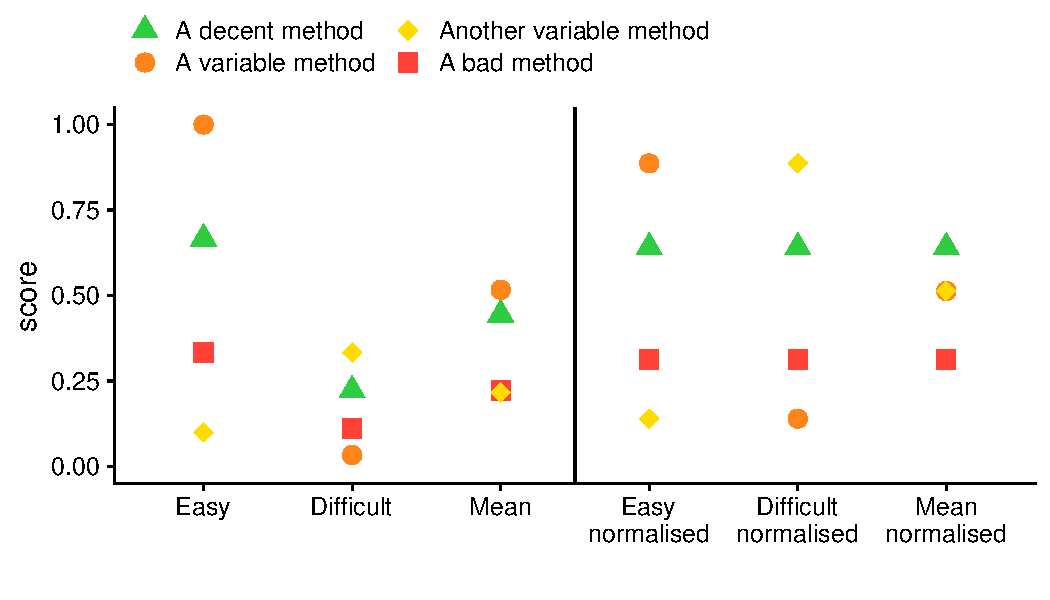
\includegraphics[width=\linewidth]{fig/snote1fig_11.pdf}
	\caption{
		\textbf{An illustration of how the difficulty of a dataset can influence the overall ranking.} 
		A decent method, which consistently ranks high on an easy and difficult dataset, does not get a high score when averaging. On the other hand, a method which ranks high on the easy dataset, but very low on the difficult dataset does get a high score on average. After normalising the scores (right), this problem disappears.
	}
	\label{fig:snote1fig_11}
\end{figure}

\begin{figure}[tbh!]
	\centering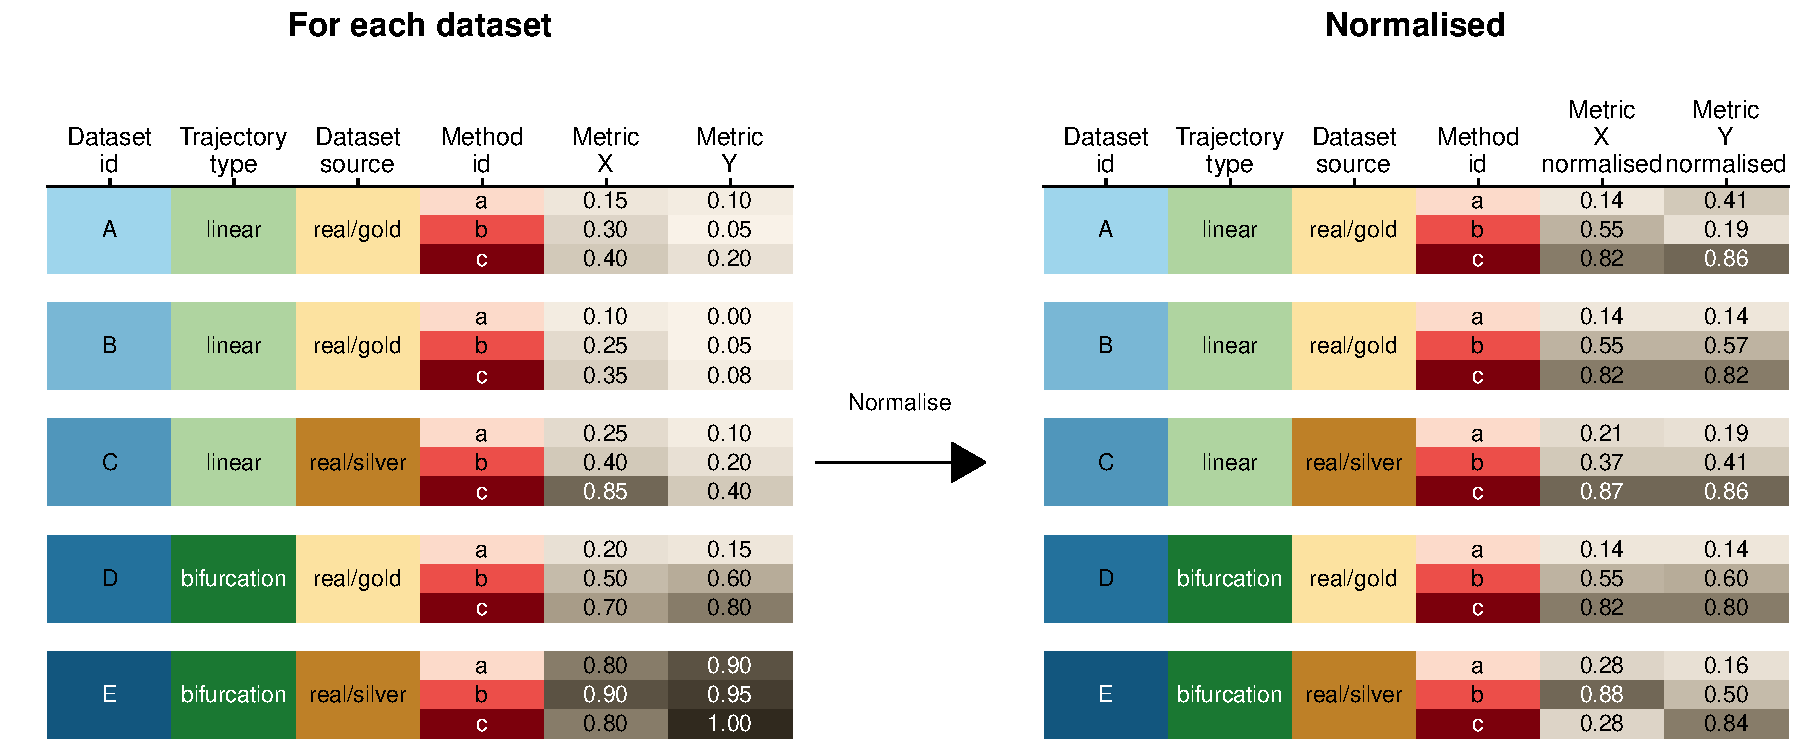
\includegraphics[width=0.8\linewidth]{fig/snote1fig_12.pdf}
	\caption{
		\textbf{An example of the normalisation procedure.} 
		Shown are some results of a benchmarking procedure, where every row contains the scores of a particular method (red shading) on a particular dataset (blue shading), with a trajectory type (green shading) and dataset source (orange shading).
	}
	\label{fig:snote1fig_12}
\end{figure}

After normalisation, we aggregate step by step the scores from different datasets. We first aggregate the datasets with the same dataset source and trajectory type using an arithmetic mean of their scores (Figure \ref{fig:snote1fig_13}a). Next, the scores are averaged over different dataset sources, using a arithmetic mean which was weighted based on how much the synthetic and silver scores correlated with the real gold scores (Figure \ref{fig:snote1fig_13}b). Finally, the scores are aggregated over the different trajectory types again using a arithmetic mean (Figure \ref{fig:snote1fig_13}c).

\begin{figure}[tbh!]
	\centering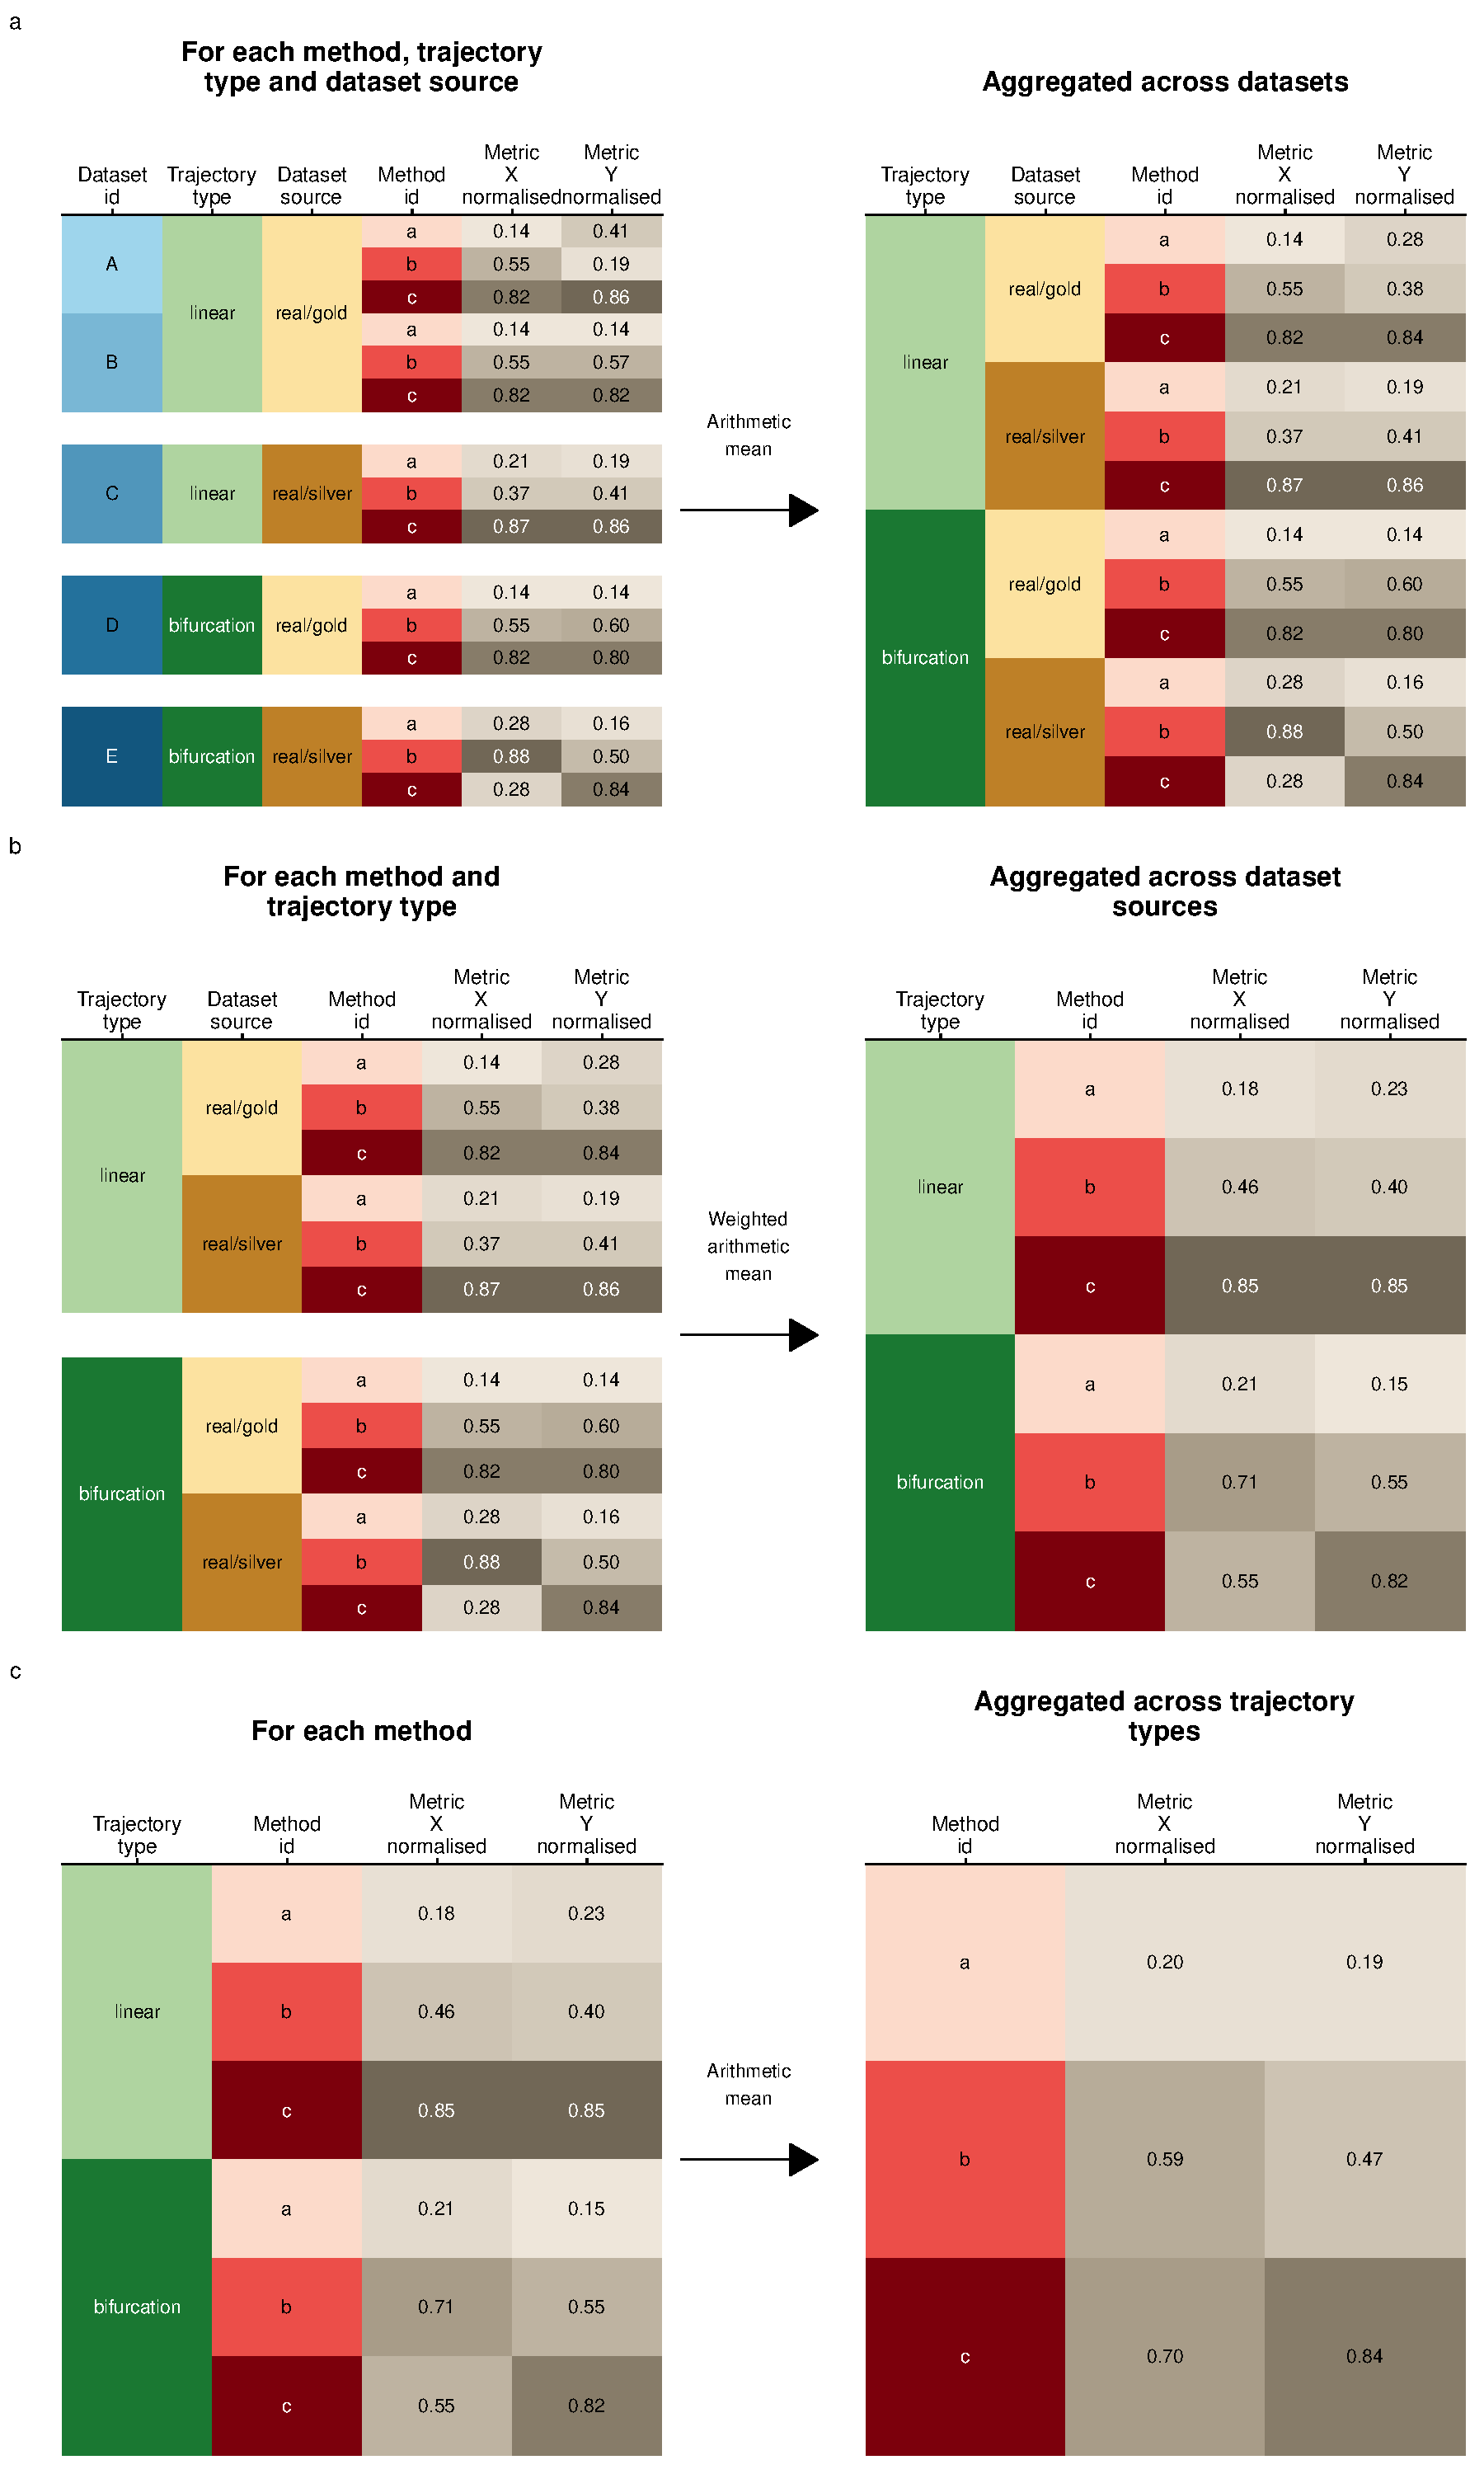
\includegraphics[width=0.8\linewidth]{fig/snote1fig_13.pdf}
	\caption{
		\textbf{An example of the aggregation procedure.} 
		In consecutive steps we aggregated across \textbf{(a)} different datasets with the same source and trajectory type, \textbf{(b)} different dataset sources with the same trajectory type (weighted for the correlation of the dataset source with the real gold dataset source) and \textbf{(c)} all trajectory types.
	}
	\label{fig:snote1fig_13}
\end{figure}

\subsubsection{Overall metrics}

Undoubtedly, a single optimal overall metric does not exist for trajectories, as different users may have different priorities:

\begin{itemize}
	\item A user may be primarily interested in defining the correct topology, and only use the cellular ordering when the topology is correct
	\item A user may be less interested in how the cells are ordered within a branch, but primarily in which cells are in which branches
	\item A user may already know the topology, and may be primarily interested in finding good features related to a particular branching point
\end{itemize}

Each of these scenarios would require a combinations of \textit{specific} and \textit{application} metrics with different weights. To provide an "overall" ranking of the metrics, which is impartial for the scenarios described above, we therefore chose a metric which weighs every aspect of the trajectory equally:

\begin{itemize}
	\item Its \textbf{ordering}, using the $\textit{cor}_{\textit{dist}}$
	\item Its \textbf{branch assignment}, using the $\textit{F1}_{\textit{branches}}$
	\item Its \textbf{topology}, using the $\textit{HIM}$
	\item The accuracy of \textbf{differentially expressed features}, using the $\textit{wcor}_{\textit{features}}$
\end{itemize}

Next, we considered three different ways of averaging different scores: the arithmetic mean, geometric mean and harmonic mean. Each of these types of mean have different use cases. The harmonic mean is most appropriate when the scores would all have a common denominator (as is the case for the $\textit{Recovery}$ and $\textit{Relevance}$ described earlier). The arithmetic mean would be most appropriate when all the metrics have the same range. For our use case, the geometric mean is the most appropriate, because it is low if one of the values is low. For example, this means that if a method is not good at inferring the correct topology, it will get a low overall score, even if it performs better at all other scores. This ensures that a high score will only be reached if a prediction has a good ordering, branch assignment, topology, and set of differentially expressed features.

The final overall score (Figure \ref{fig:snote1fig_14}) for a method was thus defined as: 

$$\textit{Overall} = \textit{mean}_{\textit{geometric}} = \sqrt[4]{\textit{cor}_{\textit{dist}} \times \textit{F1}_{\textit{branches}} \times \textit{HIM} \times \textit{wcor}_{\textit{features}}}$$

\begin{figure}[tbh!]
	\centering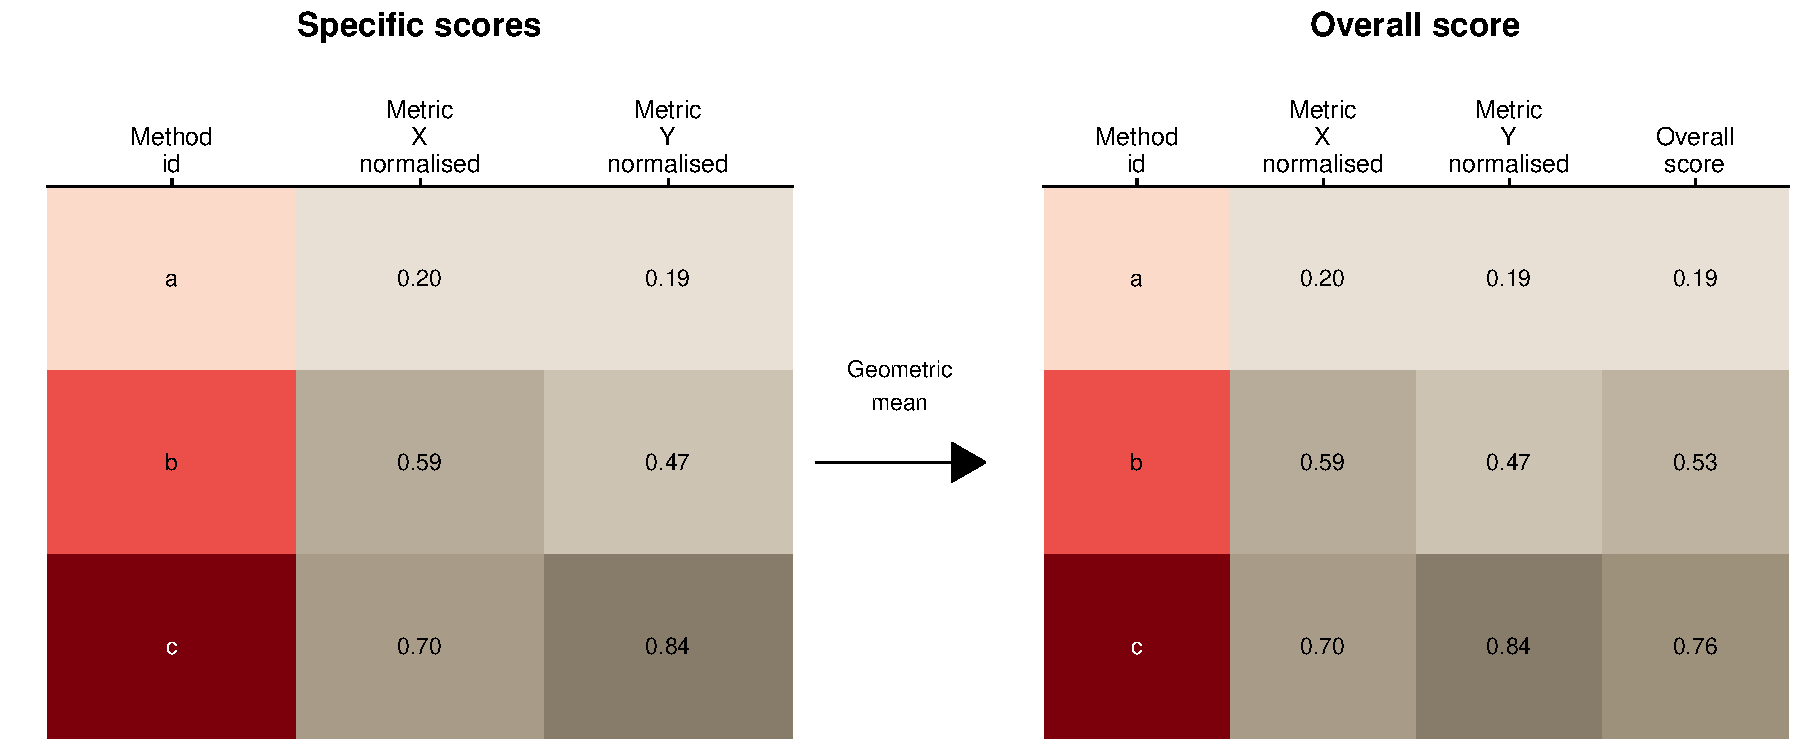
\includegraphics[width=0.8\linewidth]{fig/snote1fig_14.pdf}
	\caption{
		\textbf{An example of the averaging procedure.} 
		For each method, we calculated the geometric mean between its normalised and aggregated scores
	}
	\label{fig:snote1fig_14}
\end{figure}

We do however want to stress that different use cases will require a different overall score to order the methods. Such a context-dependent ranking of all methods is provided through the dynguidelines app (\url{http://guidelines.dynverse.org}).



\clearpage
\section{References}
\printbibliography[heading=none]

%%%%%%%%%%%%%%%%%%%%%%%%%%%%%%%%%
%%%         CH4: DYNO         %%%
%%%%%%%%%%%%%%%%%%%%%%%%%%%%%%%%%
\newpage{\thispagestyle{empty}\cleardoublepage}
\chapter{dyno: A toolkit for inferring and interpreting trajectories} 
\chaptermark{dyno: A toolkit for inferring and interpreting trajectories.} % short title
\label{chap:dyno}
\begin{quote}
	\textbf{Abstract:} \blindtext
\end{quote}
\vfill
Adapted from:\\
\textbf{Cannoodt, R.}, Saelens, W., and Saeys, Y. dyno: A toolkit for inferring and interpreting trajectories. \textit{Journal} vol, issue (2019), page--page. doi.
\blindtext

%%%%%%%%%%%%%%%%%%%%%%%%%%%%%%%%%
%%%       CH5: SCORPIUS       %%%
%%%%%%%%%%%%%%%%%%%%%%%%%%%%%%%%%
\newpage{\thispagestyle{empty}\cleardoublepage}
\chapter{SCORPIUS: Fast, accurate, and robust single-cell pseudotime} 
\chaptermark{SCORPIUS: Fast, accurate, and robust single-cell pseudotime.} % short title
\label{chap:scorpius}
\begin{quote}
	\textbf{Abstract:} \blindtext
\end{quote}
\vfill
Adapted from:\\
\textbf{Cannoodt, R.}, Saelens, W., Sichien, D., Tavernier, S., Janssens, S. Guilliams, M., Lambrecht, B., De Preter, K., and Saeys, Y. SCORPIUS improves trajectory inference and identifies novel modules in dendritic cell development. \textit{Journal} vol, issue (2019), page--page. \doi{10.1101/079509v2}.
\newpage
\graphicspath{{./ch5_scorpius/}}
\blindtext

%%%%%%%%%%%%%%%%%%%%%%%%%%%%%%%%%
%%%         CH6: BRED         %%%
%%%%%%%%%%%%%%%%%%%%%%%%%%%%%%%%%
\newpage{\thispagestyle{empty}\cleardoublepage}
\chapter{bred: Inferring single cell regulatory networks} 
\chaptermark{bred: Inferring single cell regulatory networks.} % short title
\label{chap:bred}
\begin{quote}
	\textbf{Abstract:} \blindtext
\end{quote}
\vfill
Adapted from:\\
\textbf{Cannoodt, R.}, Saelens, W., and Saeys, Y. Inferring Single Cell Regulatory Networks. \textit{Journal} vol, issue (2019), page--page. doi.
\newpage
\blindtext

%%%%%%%%%%%%%%%%%%%%%%%%%%%%%%%%%
%%%       CH7: INCGRAPH       %%%
%%%%%%%%%%%%%%%%%%%%%%%%%%%%%%%%%
\newpage{\thispagestyle{empty}\cleardoublepage}
\chapter{incgraph: Optimising regulatory networks} 
\chaptermark{incgraph: Optimising regulatory networks.} % short title
\label{chap:incgraph}
\graphicspath{{./ch7_incgraph/}}
\begin{quote}
	\textbf{Abstract:} Graphlets are small network patterns that can be counted in order to characterise the structure of a network (topology).
	As part of a topology optimisation process, one could use graphlet counts to iteratively modify a network and keep track of the graphlet counts, in order to achieve certain topological properties.
	Up until now, however, graphlets were not suited as a metric for performing topology optimisation; when millions of minor changes are made to the network structure it becomes computationally intractable to recalculate all the graphlet counts for each of the edge modifications. \\ IncGraph is a method for calculating the differences in graphlet counts with respect to the network in its previous state, which is much more efficient than calculating the graphlet occurrences from scratch at every edge modification made.
	In comparison to static counting approaches, our findings show IncGraph reduces the execution time by several orders of magnitude.
	The usefulness of this approach was demonstrated by developing a graphlet-based metric to optimise gene regulatory networks.
	IncGraph is able to quickly quantify the topological impact of small changes to a network, which opens novel research opportunities to study changes in topologies in evolving or online networks, or develop graphlet-based criteria for topology optimisation. \\
	IncGraph is freely available as an open-source R package on CRAN (incgraph). The development version is also available on GitHub (\href{http://www.github.com/rcannood/incgraph}{rcannood/incgraph}).
\end{quote}
\vfill
Adapted from:\\
\textbf{Cannoodt, R.}, Ruyssinck, J., Ramon, J., De Preter, K., and Saeys, Y. IncGraph: Incremental graphlet counting for topology optimisation. \textit{PLOS ONE} 13, 4 (2018), e0195997. \doi{10.1371/journal.pone.0195997}.
\newpage
\section*{Introduction}
Even the simplest of living organisms already consist of complex biochemical networks which must be able to respond to a variety of stressful conditions in order to survive. 
An organism can be characterised using numerous interaction networks, including gene regulation, metabolic, signalling, and protein-protein interaction. 
The advent of high-throughput profiling methods (e.g. microarrays and RNA sequencing) have allowed to observe the molecular contents of a cell, which in turn have enabled computational network inference methods to reverse engineer the biochemical interaction networks~ \cite{albert_networkinferenceanalysis_2007}.
Improving the accuracy of inferred networks has been a long-standing challenge, but the development of ever more sophisticated algorithms and community-wide benchmarking studies have resulted in significant process~ \cite{marbach_revealingstrengthsweaknesses_2010, narendra_comprehensiveassessmentmethods_2011, marbach_wisdomcrowdsrobust_2012, aijo_biophysicallymotivatedregulatory_2017}. 

Several recent developments involve incorporating topological priors, either to guide the inference process~ \cite{lopes_featureselectiontechnique_2014} or post-process the network~ \cite{ruyssinck_netterrerankinggene_2016}.
A common prior is that biological networks are highly modular~ \cite{rives_modularorganizationcellular_2003}, as they consist of multiple collections of functionally or physically linked molecules~ \cite{hartwell_molecularmodularcell_1999,barabasi_networkbiologyunderstanding_2004}. At the lowest level, each module is made up out of biochemical interactions arranged in small topological patterns, which act as fundamental building blocks~ \cite{milo_networkmotifssimple_2002}.

Graphlets~ \cite{przulj_modelinginteractomescalefree_2004} are one of the tools which could be used to add a topological prior to a biological network.
Graphlets are small connected subnetworks which can be counted to identify which low-level topological patterns are present in a network. By comparing how topologically similar a predicted network is to what would be expected of a true biological network, a predicted network can be optimised in order to obtain a better topology. 

By counting the number of occurrences of each of the different graphlets (Fig~\ref{fig_graphlets}A) touching a specific node, one can characterise the topology surrounding it. The graphlet counts of a network can be represented as a matrix with one row for each of the nodes and one column for each of the graphets (Fig~\ref{fig_graphlets}B). 
An orbit represents a class of isomorphic (i.e. resulting in the same structure) positions of nodes within a graphlet (Fig \ref{fig_graphlets}A, coloured in red).
Both graphlets and orbits have been used extensively for predicting the properties of nodes such as protein functionality~ \cite{milenkovic_uncoveringbiologicalnetwork_2008,guerrero_characterizationproteasomeinteraction_2008,singh_graphletsignaturebasedscoring_2014} and gene oncogenicity~ \cite{milenkovic_optimalnetworkalignment_2010}, by performing network alignment~ \cite{kuchaiev_topologicalnetworkalignment_2010,milenkovic_globalnetworkalignment_2013} or using them as a similarity measure in machine learning tasks~ \cite{shervashidze_efficientgraphletkernels_2009,vacic_graphletkernelsprediction_2010}. 

%% FIGURE 1
\picfig{fig/figure1.pdf}{\LARGEfigure}{fig_graphlets}{{\bf Graphlet counting in a network characterises its local topologies.}
	(A) In total, there are 30 different graphlets containing 2 to 5 nodes, ranging from $G_0$ to $G_{29}$. Orbits are an extension of graphlets which also take into account the position of a node within a graphlet. The 73 different orbits are coloured in red. (B) By counting the occurrences of these graphlets in the network, the local topology surrounding a node can be quantified.}

In this work, we focus on optimising gene regulatory networks by incorporating a topological prior as part of a topology optimisation process. We seek to optimise a predicted network by iteratively modifying the network and accepting modifications that lead to topological properties that resemble better those of true biological networks.

However, using graphlets to perform topology optimisation was hitherto not possible. Calculating the graphlet counts using the most state-of-the-art graphlet counting of a moderately sized gene regulatory network already has an execution time of about five seconds (\textit{E. coli}, $\sim 3000$ genes, $\sim 10000$ interactions, up to graphlets up to 5 nodes).
While this computational time poses no issue for regular static networks, recalculating all graphlet counts for every network modification made as part of a topology optimisation is computationally intractable. For example, performing 100'000 iterations of topology optimisation on a similarly sized network and calculating the topological impact of 10 possible edge modification at each iteration, already results in a computational time of about 12 days. Graphlet-based topology optimisation thus quickly becomes infeasible for larger networks.

When adding or removing an edge to a large network, the number of altered graphlets is much smaller than the total number of graphlets in the network. It could therefore be much more efficient to iterate over and count all the graphlets that have been added or removed as a result of the edge modification, than it is to recalculate the graphlet counts from scratch. 

Eppstein et al. introduced data structures and algorithms for updating the counts of size-three \cite{eppstein_hindexgraphits_2009} and size-four \cite{eppstein_extendeddynamicsubgraph_2012} subgraphs in a dynamic setting. The data structures were determined such that the amortised time is $O(h)$ and $O(h^2)$, respectively, where $h$ is the h-index of the network \cite{hirsch_indexquantifyindividual_2005}.

We developed IncGraph, an alternative algorithm and implementation for performing incremental counting of graphlets up to size five. We show empirically that IncGraph is several orders of magnitude faster at calculating the differences in graphlet counts in comparison to non-incremental counting approaches. In addition, we demonstrate the practical applicability by developing a graphlet-based optimisation criterion for biological networks.


\section*{Materials and methods}
Assume a network $G$ of which the graphlet counts $C_G$ are known. $C_G$ is an $n$-by-$m$ matrix, with $n$ the number of vertices in the network, $m = 73$ is the number of different orbits, and where $C_G[i,j]$ is the number of times node $i$ is part of a graphlet at orbit $O_j$. 
Further assume that one edge has either been added or removed from $G$, resulting in $G'$, at which point the counts $C_{G'}$ need to be observed. If multiple edges have been modified, the method described below can be repeated for each edge individually.

\subsection*{Incremental graphlet counting}
As stated earlier, recalculating the graphlet counts for each modification made to the network quickly becomes computationally intractable for larger network sizes. However, as the differences in topology between $G$ and $G'$ are small, it is instead possible to calculate the differences in graphlet counts $\Delta_{G, G'}$ instead. This is much more efficient to calculate, as only the neighbourhood of the modified edges needs to be explored. $C_{G'}$ can thus be calculated as $C_{G'} = C_G + \Delta_{G,G'}$.


The differences in graphlet counts $\Delta_{G, G'}$ are calculated by iterating recursively over the neighbours surrounding each of the modified edges (Fig~\ref{code_incgraph}). Several strategies are used in order to calculate $\Delta_{G,G'}$ as efficiently as possible (Fig~\ref{fig_efficient}).
(A) The delta matrix is calculated separately for each modified edge. Since the edge already contains two out of five nodes and any modified graphlet is a connected subgraph, the neighbourhood of this edge only needs to be explored up to depth 3 in order to iterate over all modified graphlets. 
(B) We propose a lookup table to look up the graphlet index of each node of a given subgraph. By weighting each possible edge in a 5-node graphlet, the sum of the edges of a subgraph can be used to easily look up the corresponding graphlet index.
(C) During the recursive iteration of the neighbourhood, the same combination of nodes is never visited twice.
(D) As the network can be relatively large, the adjacency matrix is binary compressed in order to save memory. One integer requires 4 bytes and contains the adjacency boolean values of 32 edges, whereas otherwise 32 booleans would require 32 bytes. For example, 1GB of memory is large enough to store a compressed adjacency matrix of 92681 nodes. If the network contains too many nodes to fit a compressed adjacency matrix into the memory, a list of sets containing each node's neighbours is used instead.


%% FIGURE 2
\picfig{fig/figure2.pdf}{\LARGEfigure}{fig_efficient}{{\bf Several strategies are employed in order to reduce time and memory consumption.}
(A) Only the depth 3 neighbourhood of each modified edge needs to be explored in order to have visited all modified five-node graphlets. (B) A lookup table can be used to easily look up the graphlet index of a subgraph, by weighing each edge in a 5-node subgraph by a power of~2. (C) The same combination of five nodes is never repeated, as to avoid counting the same graphlet multiple times. (D) The adjacency matrix of the network is compressed in order to reduce memory usage.}


IncGraph supports counting graphlets and orbits of subgraphs up to five nodes in undirected networks. By modifying the lookup table, the method can be easily extended to directed graphlets or larger-node graphlets, or limited to only a selection of graphlets. This allows for variations of the typical graphlets to be studied in an incremental setting.

\subsection*{Timing experiments}
We compared the execution time needed to calculate the graphlet counts in iteratively modified networks between our method and a state-of-the-art non-incremental algorithm, Orca~ \cite{hocevar_combinatorialapproachgraphlet_2014}. Orca is a heavily optimised algorithm for counting 5-node graphlets in static networks, and outperforms all other static graphlet counting algorithms by an order of magnitude~ \cite{hocevar_combinatorialapproachgraphlet_2014}.

The timing experiments were performed by generating networks from 3 different network models, making modifications to those networks while still adhering to the network model, and measuring the execution times taken for both approaches to calculate the new graphlet counts (Fig~\ref{fig_method_speedup}). 

%% FIGURE 3
\picfig{fig/figure3.pdf}{\LARGEfigure}{fig_method_speedup}{{\bf Static network model generators were modified to generate dynamic networks.}
	Three network models were used: Barabási–Albert, Erdős–Rényi, and Geometric. Step 0: a network is generated according to the network model and the given parameters. Step 1: the network is modified such that the result is as likely to have been generated by the network model. Step 2: The time for IncGraph to calculate the differences in graphlet counts is measured ($T_{IG}$). Step 3: The time for the non-incremental approach to calculate the graphlet counts of the new network is measured ($T_{NI}$). Steps 1 to 3 are repeated until all modifications generated at step 0 are processed, or until an execution time threshold has been reached.}


The network models were based on three static network models: Barab\'asi-Albert~ \cite{albert_statisticalmechanicscomplex_2002}, Erd\H{o}s--R\'enyi~ \cite{erdos_randomgraphs_1959}, and Geometric~ \cite{appel_minimumvertexdegree_1997}. These models were adapted to generate evolving networks instead (Figs~\ref{code_ba}, \ref{code_er}, and \ref{code_geo}).
Each model generates an initial network according to the static network model it is based on, and a list of network modifications (removing an edge from or adding an edge to the network). These network modifications are made such that at any given time point in the evolving network, it is likely that the network at its current state could have been generated by the original static network model.

Networks were generated with varying network models, between 1000 and 16000 nodes, node degrees between 2 and 64, and 10000 time points. We measured the time needed to calculate the delta matrix at random time points until 1 hour has passed. All timings experiments were carried out on Intel(R) Xeon(R) CPU E5-2665 $@$ 2.40GHz processors, with one thread per processor.
The generation of networks with higher node counts or degrees was constrained by the execution time of the network generators, not by IncGraph. All data and scripts are made available at \href{https://github.com/rcannood/incgraph-scripts}{github.com/rcannood/incgraph-scripts}.

\subsection*{Gene regulatory network optimisation experiments}
We demonstrate the usefulness of IncGraph by using a simple graphlet-based metric to optimise gene regulatory networks. 
One of the striking differences between real and predicted gene regulatory networks is that the predicted networks contain highly connected subnetworks, which contain high amounts of false positives.
We determine a penalty score such that predicted networks containing graphlets with many redundant edges will be penalised in comparison to very sparse networks. 

The \textit{redundancy penalty} (Fig~\ref{fig_method_reranking}A) of a network is defined as the sum of occurrences of each graphlet multiplied by the redundancy associated with each individual graphlet. The redundancy of a graphlet is the number of edges that can be removed without disconnecting the nodes from one another.
By using the redundancy penalty score, we aim to improve the gene regulatory network (Fig~\ref{fig_method_reranking}B). 

The topology optimisation procedure uses an empty network as initialisation and grows the network by selecting interactions iteratively. Each iteration, the top $k = 100$ highest ranked interactions that are not currently part of the network are evaluated, and the highest ranked interaction passing the redundancy criterion is selected (Fig~\ref{fig_method_reranking}C). This procedure is repeated until a predefined amount of time has passed.
As the aim of this experiment is not to obtain the highest performing topology optimisation method, parameter optimisation of $k$  has not been performed and is considered to be outside the scope of this work.


%% FIGURE 4
\picfig{fig/figure4.pdf}{\hugefigure}{fig_method_reranking}{{\bf Predicted gene regulatory networks of model organisms are optimised to reduce the false positive rate.}
	A)~The number of redundant edges in each graphlet are counted. B) The network is optimised in order to obtain a lower redundancy over time. Two networks are shown, one before and one after the optimisation procedure. Edges coloured in red have been removed from the network after optimisation, green edges have been added. C) Starting from an empty network, the interactions are modified by iteratively evaluating the increase in redundancy of the next $k$ interactions, and adding the first edge for which its redundancy is less than the $90^\textrm{th}$ percentile redundancy.}


We optimised gene regulatory networks of \textit{E. coli} and \textit{S. cerevisiae}. The predicted networks were generated using the network inference method GENIE3~ \cite{huynh-thu_inferringregulatorynetworks_2010} with default parameters. Gene expression data was obtained from COLOMBOS~ \cite{moretto_colombosv3leveraging_2016} and GEO~ \cite{edgar_geneexpressionomnibus_2002}, respectively. The predicted networks and the optimised versions thereof were compared against respective lists of known gene regulatory interactions~ \cite{gama-castro_regulondbversionhighlevel_2016,ma_denovolearninggenomescale_2014}.

% Results and Discussion can be combined.
\section*{Results and discussion}
The contributions of this work are twofold. Firstly, we propose a new method for incrementally calculating the differences in graphlet counts in changing graphs, and show that it is orders of magnitude faster than non-incremental approaches. Secondly, we demonstrate its applicability by optimising a predicted gene regulatory network in order to reduce the false positive rate therein.

\subsection*{Execution time is reduced by orders of magnitude}
Timing experiments show that IncGraph is significantly faster in calculating the delta matrix in comparison to calculating the graphlet counts from scratch at each iteration (Fig~\ref{fig_speedup}). The observed speedup ratios between IncGraph and the non-incremental approach Orca ranges from about 50$\times$ to 10000$\times$. The speedup ratio increases as the network size increases. For larger networks, IncGraph can thus calculate the delta matrices of 10000 edge modifications while the non-incremental approach calculates one graphlet count matrix.

Surprisingly, IncGraph obtains higher execution times for networks with 5657 nodes than for networks with 8000 nodes. One possible explanation is that the size of the data structures containing those networks are particularly favourable in avoiding cache misses. Confirmation of this explanation, however, would require further investigation.

%% FIGURE 5
\picfig{fig/figure5.pdf}{\LARGEfigure}{fig_speedup}{{\bf IncGraph is significantly faster than non-incremental approaches.}
	For small networks, the execution time of IncGraph $T_{IG}$ is already 50 times less than that of non-incremental approaches $T_{NI}$. This ratio increases even further for networks with higher numbers of nodes or higher average degrees.}


Comparing the execution time of IncGraph to the h-index of the networks indicates that the amortised time of IncGraph could be $O(h^3)$ (Fig~\ref{sfig_hindex}). This is in line with the amortised times $O(h)$ and $O(h^2)$ of the algorithm described by Eppstein et al. \cite{eppstein_extendeddynamicsubgraph_2012} for counting three-size and four-size subgraphs respectively.

\subsection*{IncGraph allows for better regulatory network optimisation}
We implemented a graphlet-based optimisation algorithm for improving the false positive rate of the predicted gene regulatory networks of \textit{E. coli} and \textit{S. cerevisiae}. After reranking the regulatory interactions, the F1 score of the first 1000~interactions had increased by 7.6\% and 2.2\% respectively (Fig~\ref{fig_reranking}A). The obtained speedup of about 15-30$\times$ (Fig~\ref{fig_reranking}B) is in line with the experiments on \textit{in silico} networks.
Namely, for the \textit{E. coli} network at 9618~interactions and 889~nodes (average degree~=~10.8), a speedup of about 30$\times$ was obtained.
Similarly, for the \textit{S. cerevisiae} network at 8013~interactions and 1254~nodes (average degree~=~6.4), a speedup of about 15$\times$ was obtained.
These speedups are in the same order of magnitude of similarly sized networks (1000~nodes and 8000~interactions) generated with a Barab\'asi-Albert model, with a speedup of 65$\times$. This is to be expected, as such networks share the same scale-free property that gene regulatory networks have.


%% FIGURE 6
\picfig{fig/figure6.png}{\Largefigure}{fig_reranking}{{\bf A simple graphlet-based scoring method improves predicted regulatory networks.}
	(A) The F1 score was calculated by calculating the harmonic mean of the AUROC and AUPR scores of the first 1000 interactions. (B) IncGraph is significantly faster than the non-incremental approach. Note that for each interaction added to the network, the graphlet counts of 100 putative interactions were evaluated.}

\section*{Conclusion}
Many improvements over the past few years have resulted in efficient graphlet counting algorithms, even for large static networks. However, needing to perform the simplest of tasks tens of thousands of times quickly becomes computationally intractable. As such, recalculating the graphlet counts of a network after each of the many network modification is infeasible.

This study introduces a method for calculating the differences in graphlet (and orbit) counts, which we call incremental graphlet counting or IncGraph for short. We show that IncGraph is at least 10-100 times faster than non-incremental methods for networks of moderate size, and that the speedup ratio increases even further for larger networks. 
To demonstrate the applicability of IncGraph, we optimised a predicted gene regulatory network by enumerating over the ranked edges and observing the graphlet counts of several candidate edges before deciding which edge to add to the network.

IncGraph enables graphlet-based metrics to characterize online networks, e.g. in order to track certain network patterns over time, as a similarity measure in a machine learning task, or as a criterion in a topology optimisation.


\section{Supporting information}

\newcommand{\pluseq}{\mathrel{+}=}
\newcommand{\asteq}{\mathrel{*}=}

\begin{figure}[htb!]
	\centering
	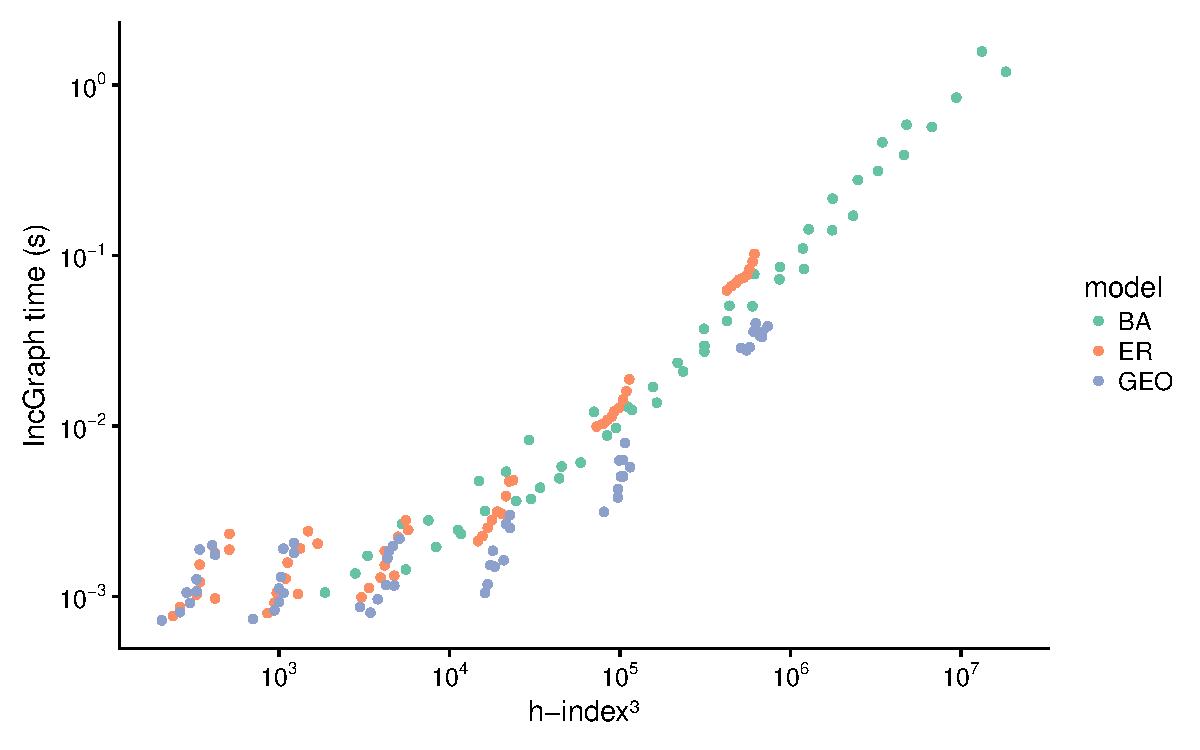
\includegraphics[width=.8\linewidth]{fig/figureS1.pdf} 
	\caption{
		\textbf{Empirical measurements show a strong relation between the execution time of IncGraph and the h-index cubed of the network it was applied to.} This is in line with the findings by Eppstein et al., where counting 3-size subgraphs has an amortised time of $O(h)$ and counting 4-size subgraphs has an amortised time of $O(h^2)$.
	}
	\label{sfig_hindex}
\end{figure}

\begin{figure}[htb!]
	\small
	\begin{algorithmic}
		\Function{CalculateDelta}{Network $G'$, Node $n_0$, Node $n_1$}
		\State \Comment{Assuming an edge $(n_0, n_1)$ has just been added or removed from $G'$}
		\State $\Delta^- \gets \Call{Matrix}{\Call{NumNodes}{G}, 73}$ \Comment{For storing the orbit counts of the removed graphlets}
		\State $\Delta^+ \gets \Call{Matrix}{\Call{NumNodes}{G}, 73}$ \Comment{For storing the orbit counts of the added graphlets}
		\State $B_0 = \{n_0, n_1\}$ \Comment{A blacklist of nodes not to visit anymore}
		\State $e = (n_0, n_1)$ \Comment{Different name for the edge}
		\If{$e \in N'$}
		\State $(m^-, m^+) = (0, 1)$ \Comment{In other words, $m^- = 1$ iff $e \in N$ and $m^+ = 1$ iff $e \in N'$}
		\Else
		\State $(m^-, m^+) = (1, 0)$
		\EndIf
		\State $x_0 = 0$
		\State $(\Delta^+, \Delta^-) = \Call{CountOrbits}{\Delta^+, \Delta^-, (n_0, n_1), x_0, m^-, m^+}$ \Comment{Update delta matrices for current nodes}
		
		%\For{$n_2 \in \Call{Neighbours}{S_0}$}
		\For{$n_2 \in \bigcup_{i \in \{0, 1\}}\Call{Neighbours}{n_i}$}
		\If{$n_2 \not\in B_0$}
		\State $B_0 = \{n_2\} \bigcup B_0$ \Comment{Add $n_2$ to blacklist $B_0$}
		\State $x_1 = x_0 + \Call{W}{G', (n_0, n_2), 1} + \Call{W}{G', (n_1, n_2), 2}$ \Comment{Calculate edge weights for current nodes}
		\State $(\Delta^+, \Delta^-) = \Call{CountOrbits}{\Delta^+, \Delta^-, (n_0, n_1, n_2), x_1, m^-, m^+}$
		\State $B_1 = B_0$ \Comment{Make a copy for the next iteration depth}
		\For{$n_3 \in \bigcup_{i \in \{0, 1, 2\}}\Call{Neighbours}{n_i}$}
		\If{$n_3 \not\in B_1$}
		\State $B_1 = \{n_3\} \bigcup B_1$
		\State $x_2 = x_1 + \Call{W}{G', (n_0, n_3), 3} + \Call{W}{G', (n_1, n_3), 4} + \Call{W}{G', (n_2, n_3), 5}$
		\State $(\Delta^+, \Delta^-) = \Call{CountOrbits}{\Delta^+, \Delta^-, (n_0, n_1, n_2, n_3), x_2, m^-, m^+}$
		\State $B_2 = B_1$
		
		\For{$n_4 \in \bigcup_{i \in \{0, 1, 2, 3\}}\Call{Neighbours}{n_i}$}
		\If{$n_4 \not\in B_2$}
		\State $B_2 = \{n_4\} \bigcup B_2$
		\State $x_3 = x_2 + \Sigma_{i \in \{0, 1, 2, 3\}}\Call{W}{G', (n_i, n_4), i+6}$
		\State $(\Delta^+, \Delta^-) = \Call{CountOrbits}{\Delta^+, \Delta^-, (n_0, n_1, n_2, n_3, n_4), x_3, m^-, m^+}$
		\EndIf
		\EndFor
		\EndIf
		\EndFor
		\EndIf
		\EndFor
		\EndFunction
		\Function{CountOrbits}{$\Delta^+$, $\Delta^-$, Nodes $S$, Edgeweights $x$, Modifier $m^-$, Modifier $m^+$}
		\State $L^- = L[x + m^-]$ \Comment{Look up the orbits of the subgraph induced by $S$ in $N$}
		\State $\Delta^-[S, L^-] \pluseq 1$ \Comment{Increment orbit counts of nodes $S$ at positions $L^-$ in $\Delta^-$}
		\State $L^+ = L[x + m^+]$ \Comment{Look up the orbits of the subgraph induced by $S$ in $N'$}
		\State $\Delta^+[S, L^+] \pluseq 1$ \Comment{Increment orbit counts of nodes $S$ at positions $L^+$ in $\Delta^+$}
		\State \Return $(\Delta^-, \Delta^+)$
		\EndFunction
		\Function{W}{Network $G$, Edge $e$, Exponent $i$}
		\State \Return $e \in \Call{Edges}{G} \ ?\  2^i : 0$ \Comment{Return $2^i$ if $G$ contains edge $e$}
		\EndFunction
	\end{algorithmic}
	\caption{
		\textbf{Pseudocode of IncGraph.} IncGraph calculates $\Delta_{G,G'}$ using a strict branch-and-bound strategy.
	}
	\label{code_incgraph}
\end{figure}

\begin{figure}[htb!]	
	\small
	\begin{algorithmic}
		\Function{BarabasiAlbert}{number of nodes $n$, degree $d$, \par\hspace*{3.72cm} number of operations $o$, offset exponent $x=1$}
		\State $D \gets \Call{Rep}{0, n}$ \Comment{All nodes start with 0 degree}
		\State $T \gets \Call{Rep}{\{\}, n}$ \Comment{List of targets of each node}
		\State $S \gets \Call{Rep}{\{\}, n}$ \Comment{List of sources of each node}
		\State $O \gets (\,)$ \Comment{Variable to store the generated operations in}
		
		\Procedure{AddEdge}{node $i$, node $j$, add as operation $b$}
		\State $D[i] \gets D[i] + 1$;\ $D[j] \gets D[j] + 1$ \Comment{Update degrees}
		\State $T[i] \gets T[i] \cup \{j\}$;\ $S[j] \gets S[j] \cup \{i\}$ \Comment{Update targets and sources}
		\If{$b$}
		\State $O \gets O + (\textrm{ADD}, (i, j))$
		\EndIf
		\EndProcedure
		\Procedure{RemoveEdge}{node $i$, node $j$, add as operation $b$}
		\State $D[i] \gets D[i] - 1$;\ $D[j] \gets D[j] - 1$ \Comment{Update degrees}
		\State $T[i] \gets T[i] \setminus \{j\}$;\ $S[j] \gets S[j] \setminus \{i\}$ \Comment{Update targets and sources}
		\If{$b$}
		\State $O \gets O + (\textrm{REM}, (i, j))$
		\EndIf
		\EndProcedure
		\Procedure{AddNode}{node $i$, add as operations $b$}
		\State $C \gets \{j \,|\, 0 \leq j < i \wedge j \not\in S[i]\}$ \Comment{Select candidate neighbours}
		\State $W \gets (D[C] \,/\, \Sigma D[C])^x$ \Comment{Calculate weights for preferred attachment}
		\State $X \gets $ sample $d$ neighbours from $C$ with weights $W$
		\For{$j \in X$}
		\State \Call{AddEdge}{$i$, $j$, $b$}
		\EndFor
		\EndProcedure
		\Procedure{RemoveNode}{node $i$, add as operations $b$}
		\While{$|T[i]| > 0$}
		\State $j \gets \Call{Head}{T[i], 1}$
		\State \Call{RemoveEdge}{$i$, $j$, $b$}
		\EndWhile
		\EndProcedure
		\For{$i \in \{1 \,..\, m\}$}
		\For{$j \in \{0 \,..\, i-1\}$}
		\State \Call{AddEdge}{$i$, $j$, false} \Comment{Start with $m+1$ complete graph}
		\EndFor
		\EndFor
		\For{$i \in \{m+1\,..\,n-1\}$}
		\State \Call{AddNode}{$i$, false} \Comment{Add the rest of the nodes}
		\EndFor
		\State $G_0 \gets \{ (i, j) \,|\, i \in \{0\,..\,n-1\} \wedge j \in N[i]\}$ \Comment{Initial network}
		\While{$|O| < o$} \Comment{Modify network until $O$ is sufficiently large}
		\State $i \gets$ Sample 1 index from $\{0 \,..\, n-1\}$
		\State \Call{RemoveNode}{$i$, true}
		\State \Call{AddNode}{$i$, true}
		\EndWhile
		\State $O \gets \Call{Head}{O, o}$ 
		\State \Return $(N_0, O)$ \Comment{Return the initial network and $o$ operations}
		\EndFunction
	\end{algorithmic}
	\caption{
		\textbf{Pseudo code for generating an evolving Barab\'asi-Albert (BA) network.} It first generates a BA network, and then generates $o$ operations such that at any time point, the network is or very closely resembles a BA network.
	}
	\label{code_ba}
\end{figure}


\begin{figure}[htb!]
	\small
	\begin{algorithmic}
		\Function{ErdosRenyi}{number of nodes $n$, number of edges $e$, number of operations $o$}
		\State $P \gets \{(i, j) \,|\, i \in \{1 \,..\, n-1\} \wedge j \in \{0 \,..\, i-1\}\}$ \Comment{All possible interactions}
		\State $N_0 \gets$ Sample $e$ edges from $P$
		\State $N_c \gets N_0$
		\While{$|O|<o$}
		\State $e_a \gets $ Sample 1 edge from $P \setminus N_c$
		\State $e_r \gets $ Sample 1 edge from $N_c$
		\State $N_c \gets (N_c \setminus e_r) \cup \{e_a\}$
		\State $O \gets O + ((\textrm{ADD}, e_a), (\textrm{REM}, e_r))$
		\EndWhile
		\State $O \gets \Call{Head}{O, o}$ 
		\State \Return $(N_0, O)$ \Comment{Return the initial geometric network and $o$ operations}
		\EndFunction
	\end{algorithmic}
	\caption{
		\textbf{Pseudo code for generating an evolving Erd\H{o}s--R\'enyi (ER) network.} It first generates an ER network, and then generates $o$ operations such that at any time point, the network is or very closely resembles an ER network.
	}
	\label{code_er}
\end{figure}

\begin{figure}[htb!]
	\small
	\begin{algorithmic}
		\Function{Geometric}{number of nodes $n$, number of edges $e$, \par\hspace*{2.77cm} number of operations $o$, number of dimensions $d=3$}
		\State $P \gets$ Sample $n$ points from a multivariate continuous uniform distribution $U_{d}((0,1)^{d})$
		\State $D \gets$ Calculate distance matrix from $P$
		\State $N_0 \gets \Call{Head}{\Call{ArgSort}{\Call{LowerTriangle}{D}}, e}$ \Comment{Initial network}
		\State $N_p \gets N_0$
		\State $O \gets (\,)$ \Comment{Variable to store the generated operations in}
		\While{$|O| < o$} \Comment{Modify network until $O$ is sufficiently large}
		\State $i \gets $ Sample 1 index from $\{0\,..\,n-1\}$
		\State $P[i] \gets$ Sample 1 point from a $U_{d}((0,1)^{d})$ \Comment{Give node $i$ a new location}
		\State $D[i,] \gets D[,i] \gets $ Calculate new distances between node $i$ and all other nodes
		\State $N_c \gets \Call{Head}{\Call{ArgSort}{\Call{LowerTriangle}{D}}, e}$ \Comment{New network}
		\State $O_a \gets \{(\textrm{ADD}, e) \,|\, e \not\in E(N_p) \wedge e \in E(N_c) \}$ \Comment{Gather added edges}
		\State $O_r \gets \{(\textrm{REM}, e) \,|\, e \in E(N_p) \wedge e \not\in E(N_c) \}$ \Comment{Gather removed edges}
		\State $O \gets O + \Call{Shuffle}{O_a + O_r}$ \Comment{Append new operations to $O$}
		\State $N_p \gets N_c$
		\EndWhile
		\State $O \gets \Call{Head}{O, o}$ 
		\State \Return $(N_0, O)$ \Comment{Return the initial geometric network and $o$ operations}
		\EndFunction
	\end{algorithmic}
	\caption{
		\textbf{Pseudo code for generating an evolving geometric network.} It first generates a geometric network, and then generates $o$ operations such that at any time point, the network is or very closely resembles a geometric network.
	}
	\label{code_geo}
\end{figure}


\clearpage
\section{References}
\printbibliography[heading=none]


%%%%%%%%%%%%%%%%%%%%%%%%%%%%%%%%%
%%%       CH8: Guidelines       %%%
%%%%%%%%%%%%%%%%%%%%%%%%%%%%%%%%%
\newpage{\thispagestyle{empty}\cleardoublepage}
\chapter{Essential guidelines for computational method benchmarking} 
\chaptermark{Essential guidelines for computational method benchmarking.} % short title
\label{chap:guidelines}
\graphicspath{{./ch8_guidelines/}}
\begin{quote}
	\textbf{Abstract:} In computational biology and other sciences, researchers are frequently faced with a choice between several computational methods for performing data analyses. Benchmarking studies aim to rigorously compare the performance of different methods using well-characterized benchmark datasets, to determine the strengths of each method or to provide recommendations regarding suitable choices of methods for an analysis. However, benchmarking studies must be carefully designed and implemented to provide accurate, unbiased, and informative results. Here, we summarize key practical guidelines and recommendations for performing high-quality benchmarking analyses, based on our experiences in computational biology.
\end{quote}
\vfill
Adapted from:\\
Weber, L. M., Saelens W., \textbf{Cannoodt, R.}, Soneson, C., Hapfelmeier, A., Gardner, P. P.,
Boulesteix, A., Saeys, Y., and Robinson, M. D.. 
Essential guidelines for computational method benchmarking. \textit{Genome Biology} 20, 125 (2019). \doi{10.1186/s13059-019-1738-8}.
\newpage
\section{Introduction}

Many fields of computational research are characterized by a growing number of available methods for data analysis. For example, at the time of writing, almost 400 methods are available for analyzing data from single-cell RNA-sequencing experiments [1]. For experimental researchers and method users, this represents both an opportunity and a challenge, since method choice can significantly affect conclusions.

Benchmarking studies are carried out by computational researchers to compare the performance of different methods, using reference datasets and a range of evaluation criteria. Benchmarks may be performed by authors of new methods to demonstrate performance improvements or other advantages; by independent groups interested in systematically comparing existing methods; or organized as community challenges. ‘Neutral’ benchmarking studies, i.e., those performed independently of new method development by authors without any perceived bias, and with a focus on the comparison itself, are especially valuable for the research community [2, 3].

From our experience conducting benchmarking studies in computational biology, we have learned several key lessons that we aim to synthesize in this review. A number of previous reviews have addressed this topic from a range of perspectives, including: overall commentaries and recommendations on benchmarking design [2, 4,5,6,7,8,9]; surveys of design practices followed by existing benchmarks [7]; the importance of neutral benchmarking studies [3]; principles for the design of real-data benchmarking studies [10, 11] and simulation studies [12]; the incorporation of meta-analysis techniques into benchmarking [13,14,15,16]; the organization and role of community challenges [17, 18]; and discussions on benchmarking design for specific types of methods [19, 20]. More generally, benchmarking may be viewed as a form of meta-research [21].

Our aim is to complement previous reviews by providing a summary of essential guidelines for designing, performing, and interpreting benchmarks. While all guidelines are essential for a truly excellent benchmark, some are more fundamental than others. Our target audience consists of computational researchers who are interested in performing a benchmarking study, or who have already begun one. Our review spans the full ‘pipeline’ of benchmarking, from defining the scope to best practices for reproducibility. This includes crucial questions regarding design and evaluation principles: for example, using rankings according to evaluation metrics to identify a set of high-performing methods, and then highlighting different strengths and tradeoffs among these.

The review is structured as a series of guidelines (Figure \ref{fig:summary_guidelines}), each explained in detail in the following sections. We use examples from computational biology; however, we expect that most arguments apply equally to other fields. We hope that these guidelines will continue the discussion on benchmarking design, as well as assisting computational researchers to design and implement rigorous, informative, and unbiased benchmarking analyses.


\begin{figure}[htb!]
	\caption{\textbf{Summary of the guidelines.} The guidelines in this review can be summarized in the following set of recommendations. Each recommendation is discussed in more detail in the corresponding section in the text.}
	\begin{tcolorbox}
		\begin{enumerate}
			\item Define the purpose and scope of the benchmark.
			\item Include all relevant methods.
			\item Select (or design) representative dataset.
			\item Choose appropriate parameter values and software versions.
			\item Evaluate methods according to key quantitative performance metrics.
			\item Evaluate secondary measures including computational requirements, user-friendliness, installation procedures, and documentation quality.
			\item Interpret results and provide recommendations from both user and method developer perspectives.
			\item Publish results in an accessible format
			\item Design the benchmark to enable future extensions.
			\item Follow reproducible research best practices, by making code and data publicly available.
		\end{enumerate}
  \end{tcolorbox}
%	\centering
%	\includegraphics[width=\hugefigure]{fig/summary_guidelines} 
%	\caption{\textbf{The workflow of dyngen is comprised of six main steps.} \textbf{A:} The user needs to specify the desired module network or use a predefined module network. \textbf{B:} Each gene in a module is is regulated by one or more transcription factors from the upstream module. Additional target genes are generated. \textbf{C:} Each gene regulatory interaction in the GRN is converted to a set of biochemical reactions. \textbf{D:} Along with the module network, the user also needs to specify the backbone structure of expected cell states. The average expression of each edge in the backbone is simulated by activating a restricted set of genes for each edge. \textbf{E:} Multiple Gillespie SSA simulations are run using the reactions defined in step C.  The counts of each of the mocules at each time step are extracted. Each time step is mapped to a point in the backbone. \textbf{F:} Multiple cells are sampled from each simulation. Molecules are sampled from each cell.}
	\label{fig:summary_guidelines}
\end{figure}


%%%%%%%%%%%%%%%%%%%%%%%%%%%%%%%%%
%%%      CH9: DISCUSSION      %%%
%%%%%%%%%%%%%%%%%%%%%%%%%%%%%%%%%
\newpage{\thispagestyle{empty}\cleardoublepage}
\chapter{Discussion and Future Perspectives} 
\chaptermark{Discussion and Future Perspectives.} % short title
\label{chap:discussion}
%dus was ik aan het nadenken over de stand van zaken na dynbenchmark ─ oké, ik heb zin om een dynbenchmark2 te doen moet, alles meer en beter
%maar hoe hebben we een impact gehad? als je kijkt naar course material over trajectory inference zou ik zeggen, veel ─ we zijn een gemakkelijke bron van guidelines
%maar als ik kijk naar de manuscripten van nieuwe TI methoden zou ik zeggen dat we nog niet zijn waar we wouden geraken

\section{Self-assessment in trajectory inference}
Many trajectory inference (TI) tools lack quantitative assessment of the accuracy of the method. Instead, they rely on anecdotal evidence to demonstrate their added value. A brief review of 76 TI articles reveals that only about 35\% contain a self-assessment (Figure \ref{fig:benchmarks_over_time}). Peer-reviewed TI articles fared even worse, self-assessing in only 32\% of cases (n=52), whereas articles first published as a pre-print self-assess in 42\% of cases (n=40). Only four TI articles feature a decently-sized comparison of at least 5 methods using 5 datasets or more.
% Note: i did not count how many metrics each of these manuscripts used.

Self-assessments are universally biased in favour of the authors, intentionally or otherwise, but this does not mean they should be skipped out on. Norel et al. provide a valuable discussion on overcoming overly optimistic self-assessments \cite{norel_selfassessmenttrapcan_2011}.
% TODO: improve working "this does not mean they should be skipped out on"

In this perspective, we hypothesise that low self-assessment rates are primarily caused by a lack of a standardised problem definition, benchmarking datasets, and metrics. 
We elaborate on these reasons and viable solutions to easy benchmarking trajectory inference.

%in deze commentary geven we nog een kort overzicht van:
%* standaard definitie van een trajectory inference probleem
%* waar kan je datasets vinden (dynbenchmark zenodo, de verschillende simulatoren, of download ze zelf van GEO)
%* hoe kan je methoden vergelijken (i.e. gebruik dynmethods)
%* wat zijn bestaande metrieken (toon overzicht van metrieken uit verschillende benchmarks en ook die van dyneval)

\begin{figure}[htb!]
	\centering
	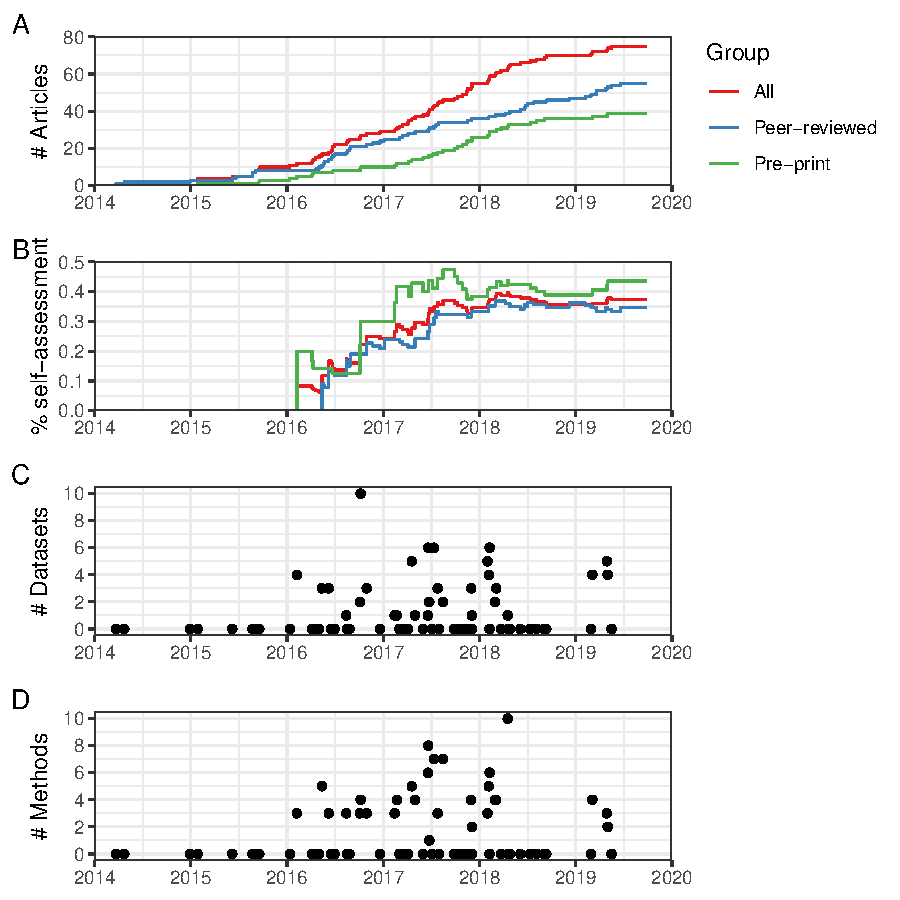
\includegraphics[width=.75\linewidth]{fig/self_assessment.pdf} 
	\caption{\textbf{The number of manuscripts featuring trajectory inference tools over time.} Areas coloured in darker shades of blue represent manuscripts containing self-assessment of the tool, highlighting \textbf{A}: the number of datasets used and \textbf{B}: the number of methods used (including the method of the authors).}
	\label{fig:benchmarks_over_time}
\end{figure}

\subsection{Problem definition}
One main reason why benchmarking TI methods is difficult is due to there being slight variations 
of the problem a method is attempting to solve (Figure \ref{fig:method_types}A). For example, a method might infer linear or cyclic trajectories, or predict the probability of a cell ending up in one of several end states.

\begin{figure}[htb!]
	\centering
	\includegraphics[width=\linewidth]{fig/method_types.pdf} 
	\caption{
		\textbf{Different forms of trajectory inference.}
		\textbf{A:} All TI methods can be categorised in one of seven subtypes in terms of its produced output \cite{saelens_comparisonsinglecelltrajectory_2019}.
		\textbf{B:} Each of these can be translated into a common format, allowing easier comparison of multiple trajectories.
		\textbf{C:} The minimum information required to describe a trajectory in this way is the milestone network -- representing transitions between cellular states -- and the cell progressions -- representing the positions of cells along the transitions.
		\textbf{D:} Optionally, regions of delayed commitment can be defined. A region of delayed commitment contain multiple transitions starting from the same milestone. This allows a TI method to assign probabilities on how likely a cell is part of one of these transitions.
	}
	\label{fig:method_types}
\end{figure}

As a result, it becomes harder to discover similar methods to compare against, as certain articles might only show up with search terms such as "pseudotemporal ordering", "lineage trees" or "fate bias". For the discoverability of a new TI method, it is therefore essential to use the term "trajectory inference", or at least list it as one of the keywords. 

A more significant and harder to solve problem is that the data formats produced by different methods varies greatly. This makes visualising and comparing multiple trajectories difficult, as different output types cannot be compared directly. The most commonly used and general is one where cells are positioned along a set of edges connecting milestones (Figure~\ref{fig:method_types}B). In practice, this format consists of two data structures: the milestone network specify transition between cell states, and the cell progressions specify how far along each cell has progressed along a transition (Figure~\ref{fig:method_types}C). Optionally, a cell can be in a region of "delayed commitment", that is, it is not known which state will end up in but a probability for ending up in either state can be assigned (Figure~\ref{fig:method_types}D). 

\texttt{dynwrap} provides implementations for converting the output from different TI subtypes into the common format. Using this standardised format allows developing reusable software for visualising (\texttt{dynplot}) and comparing (\texttt{dyneval}) trajectories from different TI methods. All of these software packages are part of the \texttt{dyno} collection, soon to be available on CRAN \cite{dyno}.

\mycomment{examples? elaborate? citation?}

\subsection{Benchmarking datasets}
Another hurdle in benchmarking trajectory inference methods is collecting datasets to benchmark against. Before 2018, there were only a handful of datasets containing complex trajectories (Figure~\ref{fig:datasets}). 

To solve this problem, benchmarking studies typically use synthetic data to complement real data. 
Several simulators have already been used to generate datasets to evaluate TI datasets, namely dyntoy \cite{saelens_comparisonsinglecelltrajectory_2019}}, dyngen \cite{dyngen}, splatter \cite{zappia_splattersimulationsinglecell_2017}, and PROSSTT \cite{papadopoulos_prossttprobabilisticsimulation_2018}.
Benefits of synthetic data are that they offer more control over the data characteristics, and that they can be generated in large quantities. This allows to evaluate performance of a method in function of a changing parameter (e.g. dataset size or noise levels), which provides information on how well the method will work on real datasets.

A common counterargument of synthetic data is that they generate unrealistic datasets and thus provide no additional value in evaluation a method. In contrast, we argue that a good set of synthetic datasets should allow benchmarkers to verify that a method should \textit{at least} work well on the synthetic datasets, but good performance on synthetic datasets does not guarantee good performance on real datasets.

By now, already hundreds of suitable real datasets exist (Figure~\ref{fig:datasets}). Downloading and pre-processing them requires a significant time investment. However, by processing the datasets once and storing them in a single repository allows them to be reused for multiple purposes. Readers are invited to reuse and extend the datasets used from our comparison of TI methods hosted on Zenodo\cite{cannoodt_singlecellomicsdatasets_2018}.

\begin{figure}[htb!]
	\centering
	\includegraphics[width=.75\linewidth]{fig/datasets.pdf} 
	\caption{\textbf{An overview collection of TI benchmarking datasets in function of their publication date and the topology of the trajectory.} These datasets are readily available on Zenodo\cite{cannoodt_singlecellomicsdatasets_2018}.}
	\label{fig:datasets}
\end{figure}


\subsection{Multiple metrics}


%waarom benchmarks een laag aantal methoden hebben:
%* iedere methode heeft zijn eigen set van functies
%* methodes hebben vaak andere prior inputs (starting cell, time series, etc)
%* methodes zijn vaak in verschillende talen geschreven (R, python, matlab)
%* de output van methodes zijn vaak niet rechtstreeks vergelijkbaar, omdat er geen standaard definitie van wat trajectory inference is (zoals bv. wel het geval is bij clustering of differential expression)
%
%bovendien is trajectory inference een probleem met complexe output, waardoor geen kant-en-klare metrieken bestonden om de predicties mee te evalueren. ik zou nog eens door alle manuscripten die een evaluatie hebben gedaan, moeten gaan, maar ik denk dat alle of toch de meeste evaluaties tussen 2016 en 2018 enkel op basis van pseudotime zijn ─ ook voor bv. dpt, en dat er maar zelden evaluaties zijn die echt gaan kijken naar de branching
%
%
%kaart aan dat we in 2018 een benchmark preprint hebben gepost van W methoden op X datasets, en in 2019 een artikel hebben gepubliceerd van Y methoden op Z datasets. Ondanks dat we in deze manuscripten de grootste problemen (# datasets, # methodes, # metrieken, leg iets beter uit) aanpakken, zien we geen vermindering in het aantal nieuwe publicaties die geen self-benchmark bevatten.
%in deze commentary geven we nog een kort overzicht van:
%* standaard definitie van een trajectory inference probleem
%* waar kan je datasets vinden (dynbenchmark zenodo, de verschillende simulatoren, of download ze zelf van GEO)
%* hoe kan je methoden vergelijken (i.e. gebruik dynmethods)
%* wat zijn bestaande metrieken (toon overzicht van metrieken uit verschillende benchmarks en ook die van dyneval)
%in conclusie, met al deze informatie melden we dat in 2019 er dus geen enkele reden is om ons te gedragen als gelijk welk ander computationeel / data mining / machine learning veld waarbij er voor quantitatief bewijs wordt gevraagd dat je methode goed werkt als je een nieuwe methode wilt publiceren. we vragen vriendelijk aan peer-reviewers om kritisch te zijn over deze kwestie.

%in deze commentary geven we nog een kort overzicht van:
%* standaard definitie van een trajectory inference probleem
%* waar kan je datasets vinden (dynbenchmark zenodo, de verschillende simulatoren, of download ze zelf van GEO)
%* hoe kan je methoden vergelijken (i.e. gebruik dynmethods)
%* wat zijn bestaande metrieken (toon overzicht van metrieken uit verschillende benchmarks en ook die van dyneval)

%in conclusie, met al deze informatie melden we dat in 2019 er dus geen enkele reden is om ons te gedragen als gelijk welk ander computationeel / data mining / machine learning veld waarbij er voor quantitatief bewijs wordt gevraagd dat je methode goed werkt als je een nieuwe methode wilt publiceren. we vragen vriendelijk aan peer-reviewers om kritisch te zijn over deze kwestie.

%refer to: \cite{norel_selfassessmenttrapcan_2011} 
%In order to alleviate the overestimation of accuracy from the many bias sources described above, we proposed a few guidelines:
%* use third‐party validation to test a model with previously unseen data
%* use more than one metric to evaluate the methods
%* report well‐performing methods even if they are not the best performers on a particular data set
%* increase the awareness of editors and reviewers that superior performance in self‐assessment is a biased demonstration of the method's value; instead, impartial assessment should be the preferred evaluation
%* Establish a scientific culture that values timely, well‐conducted follow‐up studies that confirm or refute previous results




%Before 2016, only a handful of trajectory inference methods had been released. None of these articles contained a self-benchmark simply because
%
%In all fairness towards the early TI methods, in 2016 or even 2017 there was a low abundance of good datasets to perform benchmarks with. The amount of data required to perform a comprehensive evaluation of their tool did not yet exist and was too expensive to generate. In April 2016, we started developing a single-cell simulator that would allow us to perform a comprehensive benchmark of TI methods. 
%
%
%It was also non-trivial to compare against many methods as each method has a unique interface where some prior knowledge might be needed. 
%


% * Single cell omics is expanding at rates faster than any single mind can try to conceive
%Pioneers developing revolutionary tools to process new types of data are typically faced with the problem on how to quantitatively evaluate the accuracy of their approach. After all, the amount of data required to perform a comprehensive evaluation of their tool does not yet exist and is too expensive to generate at the time. 


%In the computational jungle of single-cell omics, experts act as beacons of hope by sharing guidelines based on comprehensive benchmarking studies. Their disseminations (in the form of manuscripts \cite{lafzi_tutorialguidelinesexperimental_2018,luecken_currentbestpractices_2019}, courses \cite{kiselev_analysissinglecell_2019,martens_analysissinglecell_2019}, and slides shown during keynote caffeine refuelling sessions \cite{hemberg_coffeebreakanalysis_2019}) are crucial in leading new users, and ultimately the whole field, to better practices for performing single-cell omics analyses.

%Before embarking on this perilous adventure, I attempt to write a "Hippocratic oath for bioinformaticians", to guide me through this dissertation and not stray from the path of righteousness.
%
%\subsection{Hippocratic oath for bioinformaticians}
%We proceed with caution in developing new tools. Its results should not only be convincing and easy to interpret, but also accurate, robust, and reproducible. We open source. Our software should work reliably and fail gracefully when it does not. We acknowledge that writing automated tests is dull but necessary for maintaining long-term software projects. % TODO: improve

%Computer scientists should proceed with caution in developing new software, however, as the results produced should not only be convincing and easy to interpret, but the software should be robust and generate sufficiently accurate models of the underlying system.
%
%Bit too excited -- false positives, poor accuracy, scalability issues, poor software quality. 

\section{dyngen discussion}
% felt that upon the development of a new technologies, good quality control practices from
% other technologies were not being carried over because the data required to evaluate computational
% tools does not exist yet and is too expensive to develop.

\section{dynbenchmark discussion}
\begin{itemize}
	\item Already outdated when the manuscript was published online
	\item Update benchmark with more TI methods, newer (and larger) datasets, perform parameter optimisation on methods
	\item Include RNA velocity as inputs
\end{itemize}

\section{SCORPIUS discussion}
\begin{itemize}
	\item Extension to inferring non-linear trajectories, i.e. with principal graphs
\end{itemize}

\section{bred discussion}

%\section{incgraph discussion}

%\section{dyno discussion}




%\appendix


%\backmatter


%\printbibliography

% thanking:
% the people who brought me soup and sandwiches (look up names)
% the people who tried to use the PRISM cluster but couldn't


%Sources of funding:\\
%This study was supported by the Fonds Wetenschappelijk Onderzoek (11Y6218N) 

\end{document}
